\documentclass[11pt,a4paper]{report}
\usepackage{thesis}

\usepackage{geometry}
\geometry{tmargin=1in,rmargin=1in}

\pdfoutput=1

\setcounter{secnumdepth}{3}

% Put here some packages required or/and some personnal commands
\usepackage{ptdr-definitions}

\usepackage{calc}
\usepackage{textcomp}
\usepackage{amsmath}
\usepackage{amssymb}
\usepackage{graphicx}
\usepackage{enumerate}
\usepackage{xspace}
\usepackage{topcapt}
\usepackage{lineno}
\usepackage{subfig}
\usepackage{mathtools}
\usepackage[usenames,dvipsnames,svgnames,table]{xcolor}
\usepackage{longtable}
\usepackage{appendix}
\usepackage{multirow}
\usepackage{pifont}% http://ctan.org/pkg/pifont
\usepackage{slashed}
\usepackage{bookmark}
%\usepackage{subcaption}
%\usepackage{float}

\bookmarksetup{
  numbered,
}

\usepackage{bm}
\usepackage{rotating}

\usepackage{tikz}
\usetikzlibrary{patterns}
\usetikzlibrary{plotmarks}

\newcommand{\cmark}{\ding{51}}%
\newcommand{\xmark}{\ding{55}}%

% Local definitions.
\newcommand{\editComment}[1]{{\color{Red} #1}} % Indicates who is organising each section.

\newcommand{\ttbar}{\ensuremath{t\overline{t}}\xspace} % t-tbar
\newcommand{\ttZ}{$\text{t}\overline{\text{t}}\textrm{Z}$}
\newcommand{\ttbarZ}{$\text{t}\overline{\text{t}}\textrm{Z}$}
\newcommand{\ttW}{$\text{t}\overline{\text{t}}\textrm{W}$}
\newcommand{\ttbarW}{$\text{t}\overline{\text{t}}\textrm{W}$}
\newcommand{\ttH}{$\text{t}\overline{\text{t}}\textrm{H}$}
\newcommand{\ttbarH}{$\text{t}\overline{\text{t}}\textrm{H}$}
\newcommand{\ttbarGamma}{$\text{t}\overline{\text{t}}\gamma$}
\newcommand{\ttbarY}{$\text{t}\overline{\text{t}}\gamma$}
\newcommand{\ttY}{$\text{t}\overline{\text{t}}\gamma$}
\newcommand{\ttV}{$\text{t}\overline{\text{t}}\textrm{V}$}
\newcommand{\ttbarV}{$\text{t}\overline{\text{t}}\textrm{V}$}
 
% units
\newcommand{\T}{\unit{T}}
\newcommand{\ms}{\unit{ms}}
\newcommand{\ns}{\unit{ns}}
\newcommand{\mrad}{\unit{mrad}}
\newcommand{\Gbps}{\unit{Gb\hspace{-0.16em}/\hspace{-0.08em}s}}
\newcommand{\Tbps}{\unit{Tb\hspace{-0.16em}/\hspace{-0.08em}s}}
\newcommand{\Hz}{\unit{Hz}}
\newcommand{\kHz}{\unit{kHz}}
\newcommand{\MHz}{\unit{MHz}}
\newcommand{\GHz}{\unit{GHz}}
 
% Don't use ``c'' in GeV units, to be consistent with TDR.
\renewcommand{\GeVc}{\GeV}
\renewcommand{\GeVcc}{\GeV}

% Command definitions.
\newcommand{\pT}{\ensuremath{p_{\mathrm{T}}}\xspace}
\newcommand{\sector}{sector\xspace}
\newcommand{\segment}{\sector}
\newcommand{\qpt}{\ensuremath{q\hspace{-0.08em}/\hspace{-0.08em}\pt}\xspace}
\newcommand{\rphi}{$r$-$\varphi$\xspace}
\newcommand{\rz}{$r$-$z$\xspace}
%\newcommand{\PU}{pile-up\xspace}
\newcommand{\PU}{PU\xspace} % PU is now defined in Section 1
\newcommand{\OT}{outer tracker\xspace}
\renewcommand{\HT}{Hough Transform\xspace} % redefinition of CMS command for total transverse energy ...
\newcommand{\KF}{Kalman Filter\xspace}
\newcommand{\LR}{Linear Regression\xspace}
\renewcommand{\DR}{Duplicate Removal\xspace}
\newcommand{\MS}{multiple scattering\xspace}
\newcommand{\mat}[1]{\mathbf{#1}}
\newcommand{\combine}{\texttt{combine}}

\linespread{1.25} %% 1.5 line spacing as nominal is 1.2, ergo 1.2*1.25=1.5
\linenumbers


%%%%%%%%%%%%%%%  Title page %%%%%%%%%%%%%%%%%%%%%%%% 

% >> Title: please make sure that the non-TeX equivalent is in PDFTitle below
\begin{document}
\title{
Search for the Production of a Single Top Quark \\ in association with a Z Boson at the LHC 
}

\author{Alexander D. J. Morton}

\maketitle

\pdfbookmark[0]{Abstract}{abstract} % Sets a PDF bookmark for the abstract
\abstract{
A search for the production of a single top quark in association with a Z boson and an additional jet using data from proton-proton collisions at $\sqrt{s} = 13\TeV$ collected by the Compact Muon Solenoid (CMS) experiment at the Large Hadron Collider is presented.
This is a rare process that is predicted by the Standard Model.
This search focussed on identifying the final state containing two leptons from the Z boson decay, two jets from the decay of the W boson produced by the top quark decay, a b-jet from the top quark decay and a recoil jet.
The signal was dominated by backgrounds involving a real Z boson or two promptly produced leptons consistent with a Z boson decay, primarily Z+jet and top quark pair production.
As such, a Boosted Decision Tree was used to enhance the separation between the signal and background processes.
Using a dataset corresponding to 35.9\fbinv, signal strengths of $6.213_{-2.695}^{+2.339}$ and $4.725_{-2.015}^{+1.916}$ were measured for this process when the Z boson decays into a pair of electron or muons, respectively, and the W boson decay hadronically.
These measurements correspond to an observed (expected) signal significance of $2.722\sigma$ ($0.460\sigma$) and $2.501 \sigma$ ($0.544\sigma$), respectively, when compared to the background-only hypothesis.
These measurements are consistent within two standard deviations of the Standard Model prediction.

The CMS experiment's new tracking detector at the High-Luminosity Large Hadron Collider will require the ability to reconstruct all charged tracks with transverse momentum greater than 2-3\GeV within 4\mus so that they can be used in the Level-1 trigger decision.
One of the proposed track finders is an FPGA-based based solution using a fully time-multiplexed architecture, where track candidates are reconstructed using a projective binning algorithm based on the Hough Transform.
Studies into the suitability of a linearised $\chi^{2}$ algorithm for fitting track parameters were undertaken and it was found that its performance was inferior compared to that of a combinatorial \KF fitter.
The impact of reducing the minimum track transverse momentum from 3\GeV to 2\GeV on the proposed system was also evaluated.
The resulting degradation of performance was found to be recoverable by improving the handling of multiple scattering in the track finding and fitting algorithms.
}

\pdfbookmark[0]{Declaration of Authorship}{Declaration of Authorship} % Sets a PDF bookmark for the abstract
\chapter*{Declaration of Authorship} \label{sec:declaration}
The work described in this thesis was conducted solely by the author, except where collaboration with others occurred as stated within the text, during their time as a candidate for a research degree at this University.

Figures from CMS publications are labelled ``CMS'' or ``CMS Simulation'', when the material only includes simulated events.
Figures labelled ``CMS Preliminary'' are from an unpublished or preliminary public CMS publication.
All figures taken from external sources are referenced throughout this thesis.

The work described in Chapter~\ref{chapter:tk-upgrade} formed part of the author's contributions to \emph{TMTT} project's development of the proposed track finding system described within that chapter.
To produce the results presented in Chapter~\ref{chapter:tk-upgrade}, the author worked in collaboration with other members of the \emph{TMTT} project who were predominantly based at the University of Bristol, Brunel University London, Imperial College London, STFC Rutherford Appleton Laboratory and the Karlsruhe Institute of Technology.
In addition to the studies described in that chapter, the author's other contributions to the \emph{TMTT} project included various robustness studies and the development of the software framework used to integrate and evaluate the performance of track fitting algorithms

The author has collaborated with other members of the High Energy Physics group at Brunel University London to produce the physics analysis presented in this thesis.
The principle contributions the author made towards the analysis are described in Chapters~\ref{chapter:data-mc},~\ref{chapter:tzq-search}, and~\ref{chapter:bkg}.
The work involving the development and optimisation of the multivariate analysis technique and statistical analysis technique that was used was principally undertaken by other members of the High Energy Physics group and is described in Chapters~\ref{chapter:bkg} and~\ref{chapter:results}, respectively.


No work contained within this thesis has been submitted to this or any other university as part of the requirement for any qualification.
When the published work of others has been consulted, it has been clearly attributed within the text.


\clearpage
\newpage

\pdfbookmark[0]{Acknowledgements}{Acknowledgements} % Sets a PDF bookmark for the abstract
\chapter*{Acknowledgements} \label{sec:acknowledgments}
This thesis would not have been possible without the time, help, thoughts, and advice of many people.

First and foremost, I would like to thank my principal supervisor \textit{Joanne Cole} for her continual support, guidance and advice over the course of the last four years.
I am not sure how I can ever express my gratitude for her ability to always find time for me and for the uncountable number of times she has corrected this thesis.
I would also like to thank my second supervisor \emph{Peter Hobson} and my research development advisor \emph{David Smith} for their help and guidance through the past four years.

My thanks go to \textit{Catherine Mackay} and \textit{Corin Hoad} in particular for their work on the statistical analysis of the tZq measurement presented in this thesis.
Without both of their efforts, I suspect that the entire analysis would not be in as mature a state as it currently is.
My thanks also go to \textit{Ivan Reid} whose timely technical support and tolerance of my high bandwidth usage on the Brunel HEP group's computing resources made the work presented in this thesis possible.

I would also like to thank all those I've worked with throughout the UK CMS Collaboration and during my time at CERN, especially those from the CMS Single Top Physics community and the \emph{TMTT} collaboration.
In particular I would like to thank \textit{Andrew Rose} and \textit{Mark Pesaresi} not only for their advice throughout the last four years, but also for introducing me to \emph{High Energy Physics} in the first place.
Special thanks are warranted for \textit{Douglas Burns}, \textit{Fionn Ball}, \textit{Rachel Hyneman} and \textit{Seth Zenz} for the many enjoyable (and educational) lunches and cups of coffee we've had from across the globe.

I would like to thank all of my friends and family for their support through the years.
\textit{Darije \v{C}ustovi{c}}, \textit{Diana Lucaci}, \textit{Reuben Hill}, and \textit{Thore Bucking}; for not only occasionally providing me with a place to stay when I needed it, but whose interest in my work, no matter how seemingly banal, re-motivated me when I needed it most.
I am incredibly grateful to my Mother and Father and \textit{Annabel Shaw}; without your constant support and encouragement throughout the years, especially during the writing up of this thesis, I doubt I would have made it this far.

Finally, but most importantly, I would like to thank \textit{Peter Hobson} and the \emph{Science and Technologies Facilities Council}.
Without them, I would not have had the privilege of being able to embark on this work. 

\pdfbookmark[0]{Contents}{contents} % Sets a PDF bookmark for the abstract
\tableofcontents
\pdfbookmark[0]{List of Figures}{lof} % Sets a PDF bookmark for the abstract
\listoffigures
\pdfbookmark[0]{List of Tables}{lot} % Sets a PDF bookmark for the abstract
\listoftables

\chapter{Introduction}\label{chapter:intro}

\emph{``If I have seen further it is by standing on the shoulders of giants''}
\emph{Letter to Robert Hooke FRS, February 15th 1676, by Sir Isaac Newton FRS (1643-1727)}

The idea that nature can be explained through rational explanations, such as the ancient philosophical concepts of \emph{Atomism}and the Ancient Greek's \emph{Classical Elements}, is one that stretches back into time immemorial.

Following scientific revolution of the 17th century the scientific method replaced such philosophical reasoning as the basis of exploring the nature of reality.
By formulating hypotheses whose predictions can tested by empirical evidence, successive generations of scientists
have built upon and improved on the ideas of those before them.
By amending existing theories or proposing new theories supported by new and more precise measurements, unified descriptions of seemingly unrelated phenomena have emerged, such as James Clark Maxwell's theory of electromagnetism.
This process has taken us from John Dalton's atomic theory and Sir Isaac Newton's Laws of Motion to the Standard Model of Particle Physics in the present day, describing all known elementary particles and three of the four fundamental forces of nature.


The Standard Model has been one of the greatest and most powerful scientific theories, making predictions which have withstood incredible experimental scrutiny and been found to very accurate with very few inconsistencies with reality.
Despite these minor deviations however, there are many ... that the Standard Model cannot be a complete description of reality.
Perhaps the most glaring omission from the theory is gravity, with 

Despite the successes of General Relativity, it is irreconcilable with the Standard Model at the very high 
The strong evidence for a \emph{Dark Matter} component of the Universe to explain the 
very high energy densities where 
-Despite the successes of the Standard Model and General Relativity, they are irreconcilable at very high energy scales...
- observed oscillation of neturino flavours
- dark matter
- matter anti-matter symmetry


Increasingly powerful and luminous particle accelerators have been constructed to create the high energy environment required to probe the 

in order to provide the conditions for particle detectors to make measurements of interesting rare and short-lived physical processes against vast backgrounds of uninteresting events.

The Large Hadron Collider at CERN is 
capable of accessing physics at higher energy scales than previous colliders and producing an unprecedented amount of luminosity.


is currently the largest and most powerful particle accelerator and collider that has been built to date.
It is not only capable of accessing physics at higher energy scales than ever before, but is also capable of producing an unprecedented amount of luminosity, allowing physicists to make precise measurements and rare tests 
, but also to search for new physics beyond it.


This thesis presents a search for a predicted but undiscovered singly produced top quark process and a number of the contributions towards a study considering a potential future particle detector upgrade.

The analysis presented looks for, and makes a cross section measurement of, a single top quark which is produced in association with a Z boson in the final state involving two leptons using proton-proton collision data at $\sqrt{13}$ collected by the Compact Muon Solenoid at the Large Hadron Collider during 2016.
This process has been predicted by the Standard Model but has yet to be measured given both its rarity and similarity to more commonly produced background processes.
As the process involves the Z boson coupling between both the top quark and W boson, it is particularly sensitive to any new physics in the electroweak sector which would manifest as ..

The Compact Muon Solenoid at the High Luminosity Large Hadron Collider will require a track finding system to provide information to the trigger system in order to discriminate in favour of potentially interesting physics against increasingly large backgrounds.
During the development of one of the proposed track finding systems, studies were undertaken regarding various track fitting algorithms which would fit precise track helix parameters to the tracks found and the ability of the system to find tracks with $\pT > 3\GeVc$.
In this thesis the studies concerning the development of a Linearised $\chi^{2}$ fitter and the ability of the proposed system to find tracks with $\pT > 2GeVc$ are presented.


\section{The Standard Model of Particle Physics}\label{sec:sm}

The Standard Model (SM) is the current model which describes the fundamental matter particles of nature, fermions, and their interactions with three of the fundamental forces of nature: the weak, strong, and electromagnetic forces through force carrying particles (the gauge bosons)\cite{LagrangiansSM}.
An important property which distinguishes between the fermions and gauge bosons is spin. 
Spin is an intrinsic property of particles, with each particle having a specific quantum value, and can be likened to, despite being different from, angular momentum from classical mechanics\cite{QM}. 
The spin quantum number, $s$,  takes half-integer values, with spin z-direction, $s_{z}$, having a sign denoting whether the spin is polarised either along the same direction as the z-axis (usually a ``positive'' sign) or the opposing direction of the z-axis (usually a ``negative'' sign)\cite{QM}. 
Fermions are half-integer spin particles (i.e. s = $\pm\frac{1}{2}, \pm\frac{3}{2},\pm\frac{5}{2}$,…) which have three so-called ``generations'', and belong to one of two families: quarks and leptons\cite{ElectroweakStrong}. 
Quarks experience all of the fundamental forces of nature, whilst leptons experience all but the strong force\cite{LagrangiansSM}. 
In each generation, for fermions and quarks alike, there are two different fundamental particle\cite{LagrangiansSM}. 
Each subsequent generation of particles are identical, except for their quantum number and mass. 
Quark particles in each generation either have an electrical charge of $\frac{+2}{3}$ or $\frac{-1}{3}$ and fermions have either electrical charge -1 or 0 (neutral)\cite{ElectroweakStrong}. 

Quarks are the fundamental particles of which hadrons, composite particles formed of quarks, are formed. 
Hadrons are either mesons which are formed of two quarks or baryons which are formed of three quarks. 
Exotic hadrons formed of larger groupings (four or more) of quarks have been hypothesised, but only one resonance, namely a tetraquark candidate whose quark content still has to be confirmed, has been observed\cite{PhysRevLett.112.222002}. 
The first generation of quarks comprises of the up and down quarks, which form the protons and neutrons that are found in conventional atomic matter. 
The second and third generations are each subsequently more massive than the first generation and comprise of the strange and charm quarks and top and bottom quarks respectively. 

Each charged lepton has an associated neutral, near massless, lepton known as a neutrino. 
As neutrinos have no associated electrical charge, their only interaction with other particles in the SM is through the weak force. 
As with the quarks, each subsequent generation’s particles are more massive than the last. 
Whilst the SM assumes that neutrinos are massless, the ``Homestake'' experiment’s measurements showed that the fraction of electron neutrinos arriving from the Sun was at the most half (if not less) what was expected\cite{PhysRevLett.20.1205}. 
Neutrino flavour oscillation would explain the observed solar neutrino flux, but would require neutrinos to have a non-zero mass. 
In 2013, the T2K collaboration presented results which confirmed the existence of neutrino oscillation\cite{PhysRevD.88.032002}. 
Whilst there are upper bounds on the neutrino masses from cosmological constraints, no experiment to date has been sensitive enough to determine the masses\cite{1475-7516-2006-06-019}. 

In the SM there are four gauge bosons, each of which is an integer spin particle (i.e. 0, $\pm 1$, $\pm 2$, …) that mediate the weak, strong and electromagnetic forces. 
The photon ($\gamma$), a massless particle, mediates the electromagnetic force, the charged $W^\pm$ and neutral $Z^0$ boson mediates the weak force and eight types of gluon mediate the strong force\cite{LagrangiansSM}. 

The mathematical formulation of the SM model is through renormalisable Quantum Field Theory (QFT)\cite{LagrangiansSM}. 
QFTs treat matter as the excitation of fermionic fields which permeate the Universe. 
The Lagrangian formalisation, used in QFTs to describe the dynamics of a system, has the Lagrangian ``$L$'' described as the difference between the kinetic and potential energy of the system\cite{LagrangiansSM}. 
QFTs usually make use of the Lagrangian Density ``$\mathcal{L}$'', defined as\cite{QFT}:

\begin{equation}
L = \int \mathrm{d^{3}}x \mathcal{L}
\end{equation}

With the general form of the Lagrangian Density being defined as:

\begin{equation}
\mathcal{L} = \mathcal{L} ( \varphi_{i}, \partial _{\mu} \varphi_{i} )
\end{equation}

Where $\partial _{\mu}\varphi_{i} \equiv \partial \varphi / (\partial x^{\mu} )$ is the four-gradient of the field $\phi$ and where the i’s are implicitly summed according to Einstein summation convention\cite{ElectroweakStrong}.

The Lagrangian acts upon a system, with all information pertaining to the system’s quantum state being described by a wave function. 
The amplitude of the wave function can be interpreted as the probability amplitude from which a measurement of an observable physical quantity can be obtained\cite{Isham}. 

An important feature of modern physical theories is that the laws of physics pertaining to a system do not vary under observation – they are `invariant''. 
Examples of such invariant or conserved quantities include electrical charge from the $U(1)$ group’s symmetry in electromagnetism, energy-momentum from space-time symmetry and angular momentum from rotational symmetry\cite{Heywood}. 
These equivalent descriptions of the same system are related by groups of transformations, which if invariant when applied to the wave function, relate to observable properties\cite{QFT}. 
If the transformations on the system have no space-time dependence, the transformation is said to be ``global'', and if the transformations do have a space-time dependence then the transformation is said to be ''local''. 
A Lagrangian which has continuous local symmetry is said to be gauge invariant\cite{Heywood}. 

As defined above however, the Lagrangian Density $\mathcal{L}$ is not gauge invariant due to its dependence on the derivative $\partial _{\mu}$. To illustrate this, the Lagrangian which describes free-field fermions\cite{QFT}, 

\begin{equation}
\mathcal{L}_{0} = \bar{\psi}(i\gamma^{\mu}\partial_{\mu} - m)\psi
\end{equation}

Which when undergoing a local phase transformation,

\begin{equation}
\psi(x) \rightarrow \psi'(x) = \psi(x)e^{-ixf(x)}
\bar{\psi(x)} \rightarrow \bar{\psi'}(x) = \psi(x)e^{+ixf(x)}
\end{equation}

Transforms as:

\begin{equation}
\mathcal{L}_{0} \rightarrow \mathcal{L}_{0}' = \mathcal{L}_{0} + q \bar{psi}(x)\gamma^{\mu}\psi(x)\partial_{\mu}f(x)
\end{equation}

This transformation is clearly not invariant. Invariance can be restored by introducing a gauge field $A_{\mu}(x)$, associated with the $\psi(x)$ field, which transforms according to the gauge transformation. 
The minimal substitution in $\mathcal{L}_{0}$ which achieves this is the replacement of the derivative $\partial_{\mu}$  with the so-called ``covariant derivative''\cite{QFT}:

\begin{equation}
\partial_{\mu} \rightarrow D_{\mu} = [ \partial_{\mu} - icA_{\mu}(x) ]
\end{equation}

Which transforms as in the same way as the $\psi(x)$ field:

\begin{equation}
D_{\mu}\psi(x) \rightarrow e^{-icf(x)}D_{\mu}\psi(x)
\end{equation}

Thus the Lagrangian which describes the system in the QFT, remains invariant. 
The interaction between the vector gauge field $A_{\mu}(x)$ and the $\psi(x)$ can be interpreted as excitations in the vector field interacting with the particles described by $\psi(x)$, such as photons interacting with electrons in Quantum Electrodynamics. 
The constant c is the coupling constant for the vector field, which differs between different gauge fields. 
In the case of Quantum Electrodynamics, $c = q$, where q is the charge of an electron\cite{QFT}.

The differences between bosonic and fermionic particles can now be considered in the context of how they are affected by considering the individual particles within a system and how they are ordered. 
As particles with integer-spin must be quantised according to Bose-Einstein statistics and half-integer spin particles by Fermi-Dirac statistics, their wave functions must be symmetrical and anti-symmetrical respectively\cite{QM}:

\begin{equation}
\psi_{symmetric}(x_{a},x_{b}) = \psi_{symmetric}(x_{b},x_{a})
\psi_{anti-symmetric}(x_{a},x_{b}) = -\psi_{anti-symmetric}(x_{b},x_{a})
\end{equation}

As such, the Fermi Exclusion Principle, where two fermions are unable to exist in the same quantum state, can be formalised as\cite{QM}:

\begin{equation}
\psi_{anti-symmetric}(x_{a},x_{a}) = 0 \qquad \forall \quad a
\end{equation}

Quantum Electrodynamics (QED) is the theory which describes the Electromagnetic force between all electrically charged particles within with the SM. 
It has a single gauge boson, the neutrally charged photon. 
Because of the photon’s lack of mass, the Electromagnetic force has an infinite range. 
As mentioned above, the Electromagnetic interaction conserves electrical charge, which is described by the $U(1)_{hypercharge}$ group symmetry in QFT\cite{QFT}. 

The Weak force is responsible for weak isospin processes. 
It has three massive gauge bosons, the electrically charged $W^{\pm}$ and neutral $Z^{0}$ bosons. 
The projection of the weak isospin along the z-axis is the conserved quantity of the Weak interaction, which in QFT is described by the $SU(2)_{weak isospin}$ group symmetry. 
The range and strength of the Weak force is considerably less than that of the Electromagnetic force due to the short lifespan of the massive gauge bosons\cite{ElectroweakStrong}. 

Both the Electromagnetic and Weak interactions can be described as a single interaction: the Electroweak interaction. 
The conserved quantity of this force, the weak hypercharge, is related to the conserved quantities of electrical charge and the z-projection of weak isospin, of its two constituent interactions. 
At sufficiently high energies, the two separate manifestations of the electroweak force unify into a single force. 
However, the $SU(2)_{weak isospin} \times U(1)_{hypercharge}$ symmetry of the electroweak interaction is not exact as whilst local invariance requires that the gauge boson fields be massless in order for the QFT to be renormalisable, the $W^{\pm}$ and $Z^{0}$ bosons are relatively massive. 
In order to retain a renormalisable theory, an additional mechanism, which introduces the masses of the weak bosons, must be introduced. 
The Higgs mechanism is the simplest solution to the breaking of the symmetry of the electroweak interaction\cite{LagrangiansSM}. 

The fundamental theory of strong interactions is Quantum Chromodynamics (QCD). 
The strong force is mediated by eight massless spin-1 gluons, which acts upon the conserved strong force charge: colour\cite{ElectroweakStrong}. 
The conservation of colour is described by the $SU(3)_{colour}$ group and the symmetry is exact. 
Colour charge is unrelated to the visual perception of colour, but stems from the fact that unlike the electroweak interaction which has positive and negative charges, there are three colour charges. 
An important difference between the gauge bosons of the electromagnetic and strong forces is that whilst the photon is chargeless, gluons are not. 
Gluons carry both a colour and anti-colour charge and only interact with coloured particles (quarks and other gluons)\cite{ElectroweakStrong}. 

A phenomena unique to the strong interaction is that the effective strong interaction coupling constant $\alpha_{s}$ tends to zero as the energy scales increase, despite the gluon being massless. 
In other words, the constant $\alpha_{s}$ increases as the separation between colour charged particles increases. 
This ``asymptotic freedom'' is caused by the virtual quark-anti quark sea containing virtual gluons which increases the force between quarks for greater separations, in contrast to the screening effect of virtual electrically neutral photons in electromagnetic interactions. 
The increase in $\alpha_{s}$ with the separation between colour charged particles means all particles must be ``colourless'', with the consequence that quarks are confined to exist in bound states\cite{ElectroweakStrong}. 
If enough energy is put into a bound state, with the intent of breaking ``colour confinement'', the energy of the colour fields between the coloured particles will increase until it is more energetically favourable for quark pair production to occur than to increase the separation between the original two quarks\cite{Griffiths}. 

\subsection{Beyond The Standard Model}\label{bsm}

The SM is far from being a complete theory. 
One of the most pressing problems was that while the $SU(3)_{colour}$ symmetry is exact, the $SU(2)_{isospin} \times U(1)_{hypercharge}$ ``electroweak'' symmetry is said to be ``broken''. 
QFTs require massless vector fields in order to be locally invariant but the $W^{\pm}$ and $Z^{0}$ bosons are observed to be massive in contrast to the massless photon. 
The Higgs mechanism is the simplest solution to this paradox, with the scalar Higgs field being responsible for the massive bosons. 
Both the CMS and ATLAS experiments at CERN have independently confirmed the existence of an unknown boson at $\approx$ 125\GeV, which was later confirmed to be consistent with the Higgs Boson, the smallest possible excitation of its associated namesake field. 
Searches to determine whether this is the SM Higgs or not (several theories including SUSY propose multiple Higgs) will take place after the phase-0 upgrades of the LHC. 

Aside from electroweak symmetry breaking, there are a number of other fundamental phenomena that the SM does not account for. 
These include, but are not limited to, the lack of explanation for gravity, the lack of candidates for dark matter, and observed matter/antimatter asymmetry in the universe. 
Gravity is left unexplained as the SM, a quantum mechanical theory, is incompatible with General Relativity, a classical theory. 

Supersymmetry (SUSY), a popular extension of the SM, makes progress with these questions by proposing that every fundamental fermion has a massive boson ``superpartner'' (and vice versa for the gauge bosons). 
The superpartners generalise space-time symmetries, allowing for bosons and fermions to be related, a straightforward unification of the strengths of the weak, electromagnetic and strong interactions at high energies and a more ``natural'' emergence of the Higgs potential. 
These supersymmetric particles (sparticles) spin differs from their SM counterparts by 1/2 (ie. bosons’ supersymmetric partners are fermions, and vice versa). 
As supersymmetry is 'broken', the expected sparticle masses are considerably greater than their equivalent partner masses. 

Additionally, some SUSY models also include candidates for a dark matter particle which is consistent with observations. 
However, while superpartners should be observed at the LHC if SUSY exists at the electroweak scale, no superpartner has been observed so far, with results being used to constrain the range of the possible superpartner masses. 
If SUSY, in any of its forms, exists, then higher energy runs of the LHC will be required to illuminate it. 




\chapter{The LHC accelerator and the CMS experiment}\label{chapter:lhc-cms}
\section{The Large Hadron Collider}\label{sec:lhc}

The Large Hadron Collider (LHC) at the European Organisation for Nuclear Research (CERN)~\cite{Bruning:782076}, in Geneva, Switzerland is the highest-energy particle accelerator constructed to date. 
It is designed to operate at a centre of mass (CoM) energy of 14\TeV, through two 7\TeV proton beams travelling in 2808 bunches of up to $1.15 \times 10^{11}$ protons at a collision rate of 25\ns which corresponds to a design luminosity of $10^{34}\percms$~\cite{Bayatian:2006zz}. 
The LHC can also operate in a heavy-ion mode, where lead ions are collided at 2.76\TeV per nucleon usually for one month a year.

The beams collide at four interaction points around the LHC, with one of the four major experiments being based at each of them. 
The experiments are: A Toroidal LHC Apparatus (ATLAS)~\cite{Aad:2008zzm} and the Compact Muon Solenoid (CMS)~\cite{oldcms} detectors, which are the two multi-purpose experiments; the Large Hadron Collider beauty (LHCb)~\cite{Alves:2008zz} which is an experiment that specialises in b-physics and; A Large Ion Collider Experiment (ALICE)~\cite{Aamodt:2008zz}, which as the name suggests, specialises in heavy ion physics.
Three smaller experiments are situated close to one of the four main experiments and use the same collision points.
Both the TOTal Elastic and diffractive cross section Measurement (TOTEM)~\cite{Anelli:2008zza} and LHC-forward (LHCf)~\cite{Adriani:2008zz} experiments study diffractive physics in the very-forward regions of collisions at the CMS and ATLAS experiments' collision points respectively.
Monopole and Exotics Detector At the LHC (MoEDAL)~\cite{Pinfold:2009oia} shares the LHCb experiment's cavern and performs direct searches for magnetic monopoles and highly ionising stable and pseudo-stable massive particles.

Currently there are three planned phases of operation for the LHC~\ref{fig:lhc-planning}: ``Phase-0'' will see the preparations for 14\TeV operations; ``Phase-I'' will see the accelerator prepared for high luminosity operations; and ``Phase-II'' will see modifications for very high luminosity operations~\cite{ECFA}. Any proposed upgrades of the detectors will naturally have to coincide with the shutdowns of the LHC.

\begin{figure}[htbp]
\begin{center}
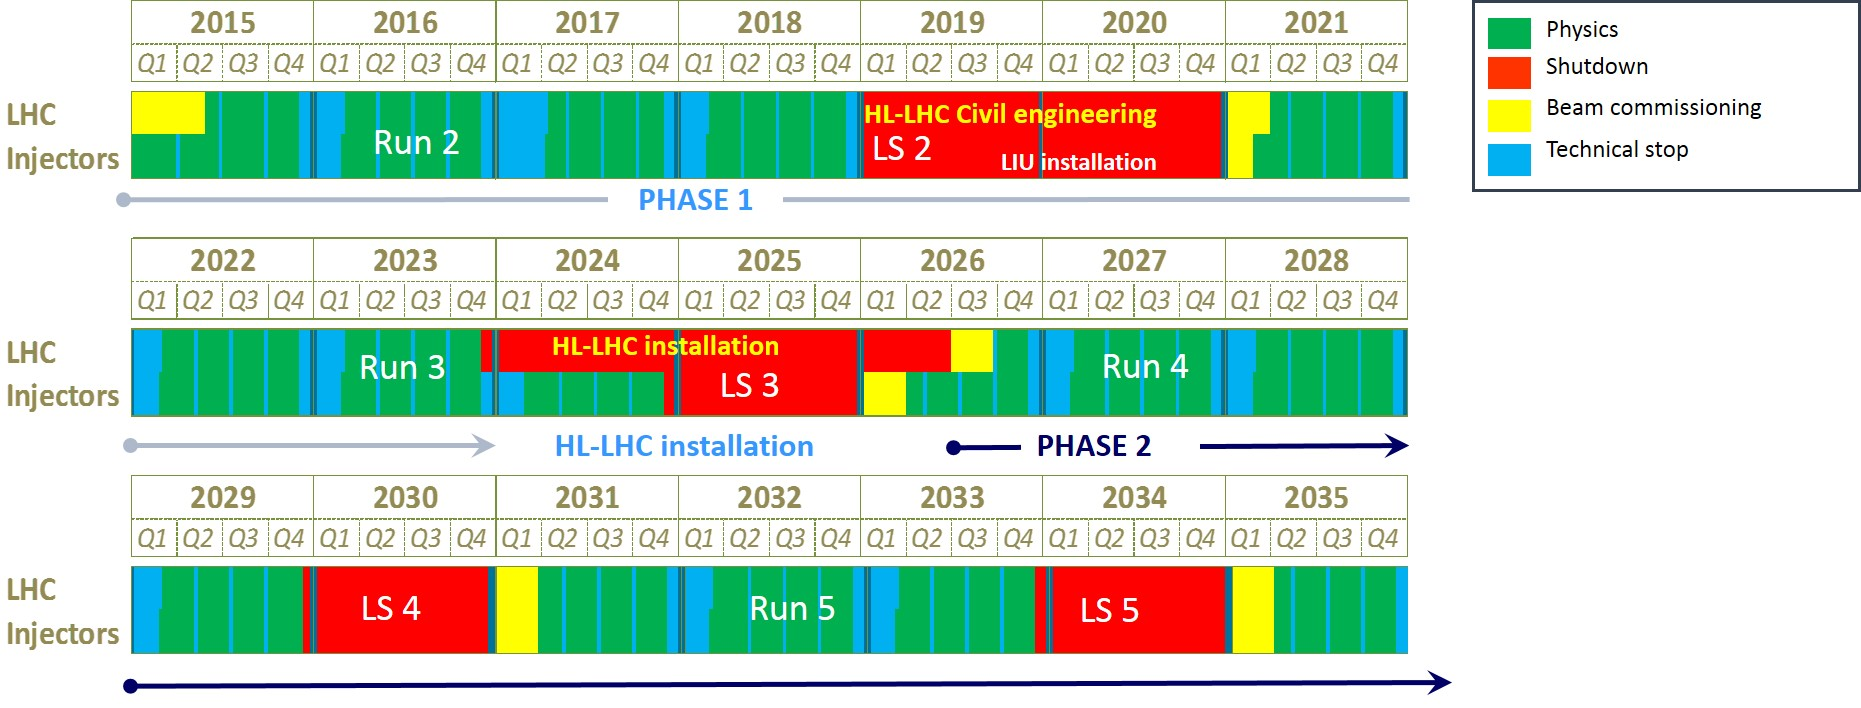
\includegraphics[width=0.97\textwidth]{figs/lhc/LHC-Planning.jpg}
\caption{Overview of the plan for the LHC and its injectors from 2015 to 2035~\cite{P2TrackerTDR}. Data taking for physics is indicated in green, long shutdowns in red, beam commissioning in yellow and technical stops in blue.}
\label{fig:lhc-planning}
\end{center}
\end{figure}

\subsection{Accelerator Complex}
When operating in proton-proton mode, the preparation of the LHC beams starts at Linear accelerator 2 (Linac2). 
Protons from a hydrogen gas source are accelerated to 50\MeV and are injected into the Proton Synchrotron Booster (PSB) which accelerates the protons to 1.4\GeV before injection into the Proton Synchrotron (PS). 
In the PS, the protons are accelerated to 26\GeV and are injected into the Super Proton Synchrotron (SPS) where they are accelerated to 450\GeV before finally entering the LHC, as illustrated in Fig.~\ref{fig:cern-accelerator-complex}. 
When operating with lead ions, Linear accelerator 3 (Linac3) is used to initially accelerate the ions before injecting them into the Proton Synchrotron Booster, before the ions use the same accelerators as the protons do to prepare them for use in the LHC~\cite{Bruning:782076}. 

Sixteen Radio Frequency (RF) cavities (eight per beam), each operating at frequency of 400\MHz, at a temperature of 4.5K, and delivering a maximum of 2 MV, are used to accelerate the two beams up to their designed operational energies of 7\TeV over the course of circa twenty minutes.
Each of the two beams are accelerated in separate beam pipes, circulating in opposite directions,and requires 1232 dipole magnets to bend them along their circular path and 392 quadrupole magnets to focus them, with each magnet producing a 8.3T field whilst operating at 1.9K.
A more detailed description of the LHC accelerator chain at CERN can be found in~\cite{Schindl:397574}. 

\begin{figure}[htbp]
\begin{center}
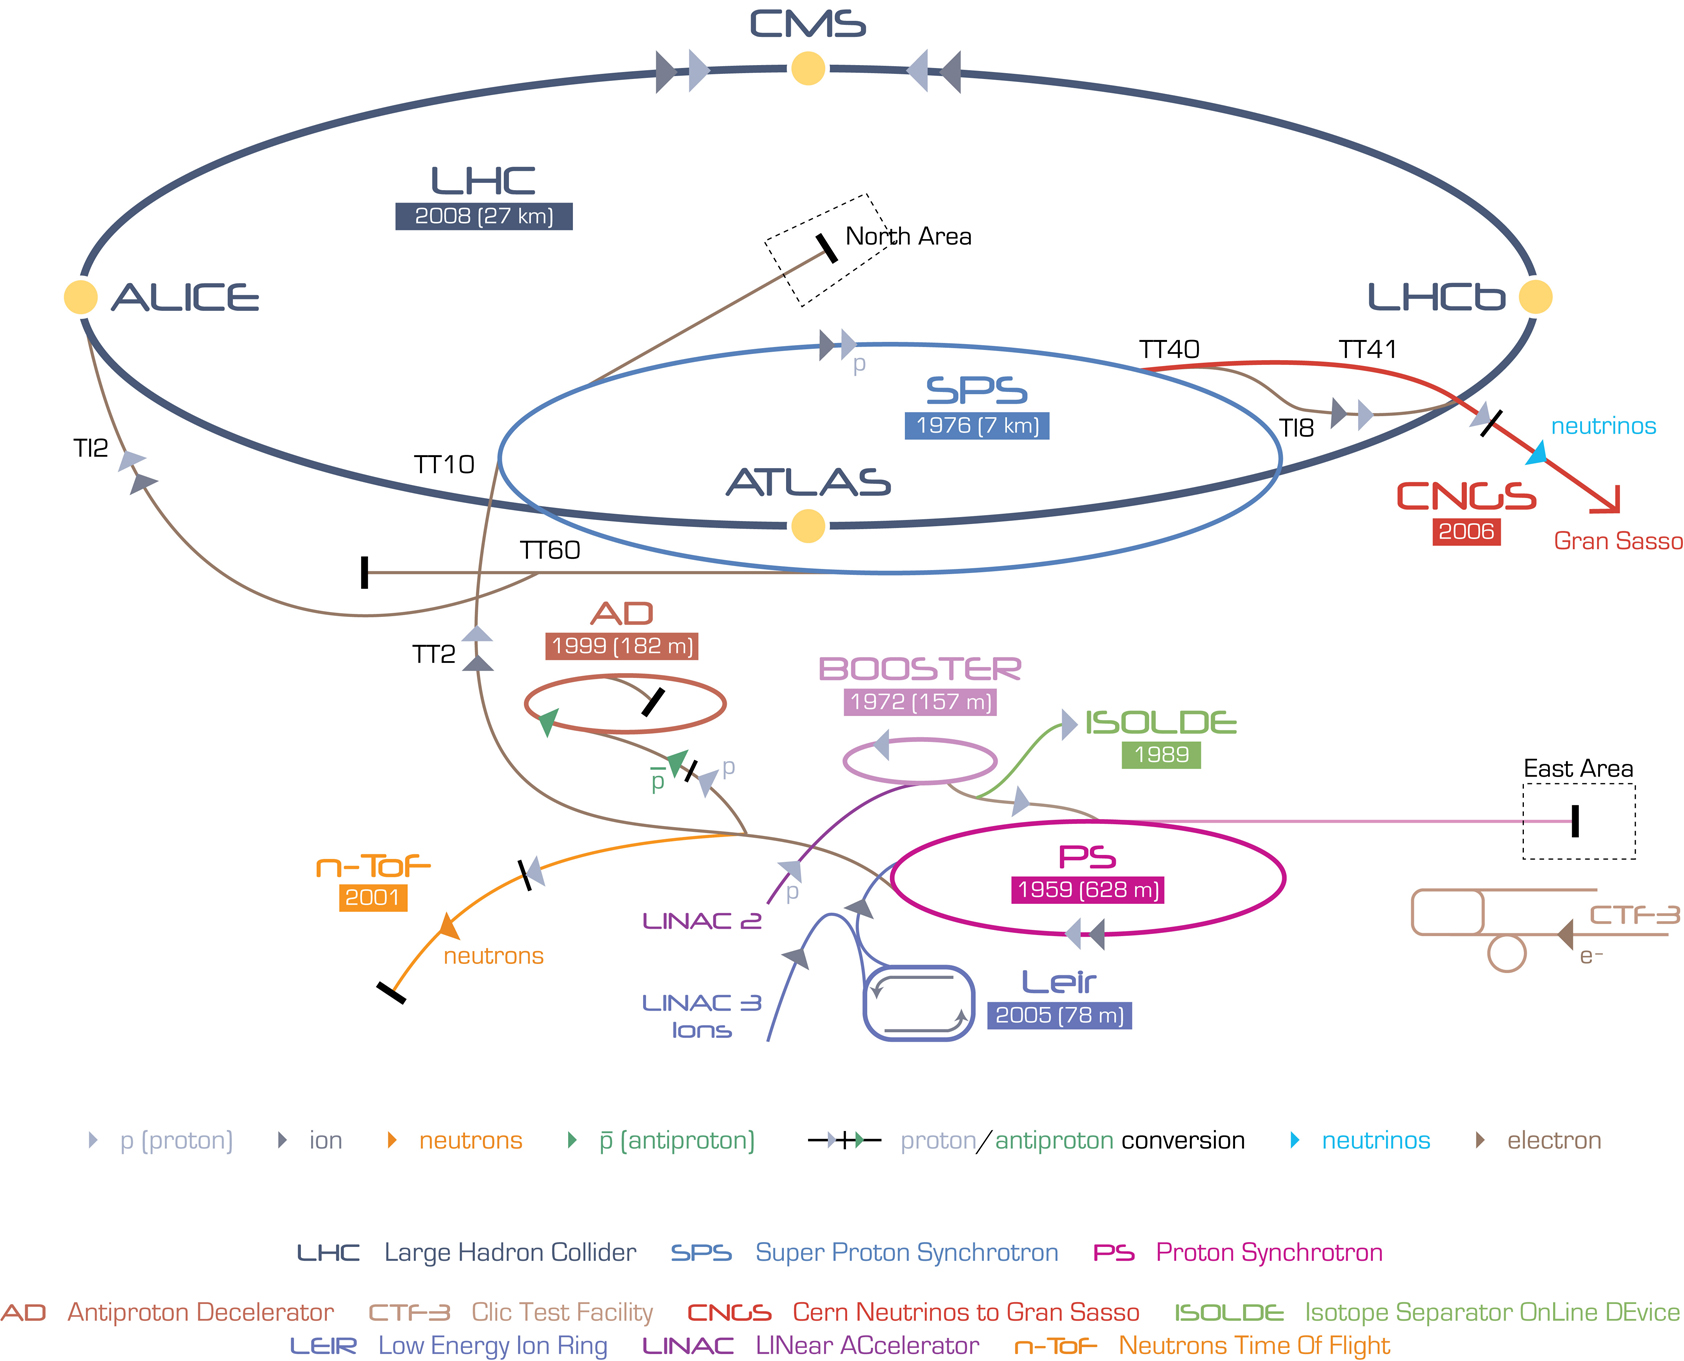
\includegraphics[width=0.97\textwidth]{figs/lhc/Cern-Accelerator-Complex.jpg}
\caption{CERN complex, including the various linear accelerators, synchrotrons, LHC, LHC detectors and other aspects of the complex.}
\label{fig:cern-accelerator-complex}
\end{center}
\end{figure}

\subsection{Motivation}
The core motivations behind the LHC are to shed light on the nature of the electroweak symmetry breaking, which the Higgs was presumed and found to be responsible for, and to probe the consistency of the SM above the \TeV level through precision measurements of SM parameters and the Higgs mechanism.
Alternative theories to the SM, such as SUSY theories, additional dimensions or new fundamental forces and particles are expected to emerge at and above the TeV level, giving the potential to ascertain whether these theories have any basis beyond mere conjecture~\cite{Bayatian:2006zz}.

In order to explore and permit the discovery of physics at the \TeV level, the total centre of mass energy has to be greater than the energy region being explored as, due to the composite nature of the proton, only a fraction of the collision centre of mass energy is available.
Access to physics beyond the \TeV level is not excluded	however, as some signals would be ``unmissable'', but the majority of physics would be limited by statistics.
Compared to the total inelastic cross section, the production cross section of the Higgs boson and hypothesised SUSY particles, if they have \TeV masses (and exist), are predicted to be many orders of magnitude smaller (see Fig.~\ref{fig:crossSections}).

\begin{figure}[htbp]
\begin{center}
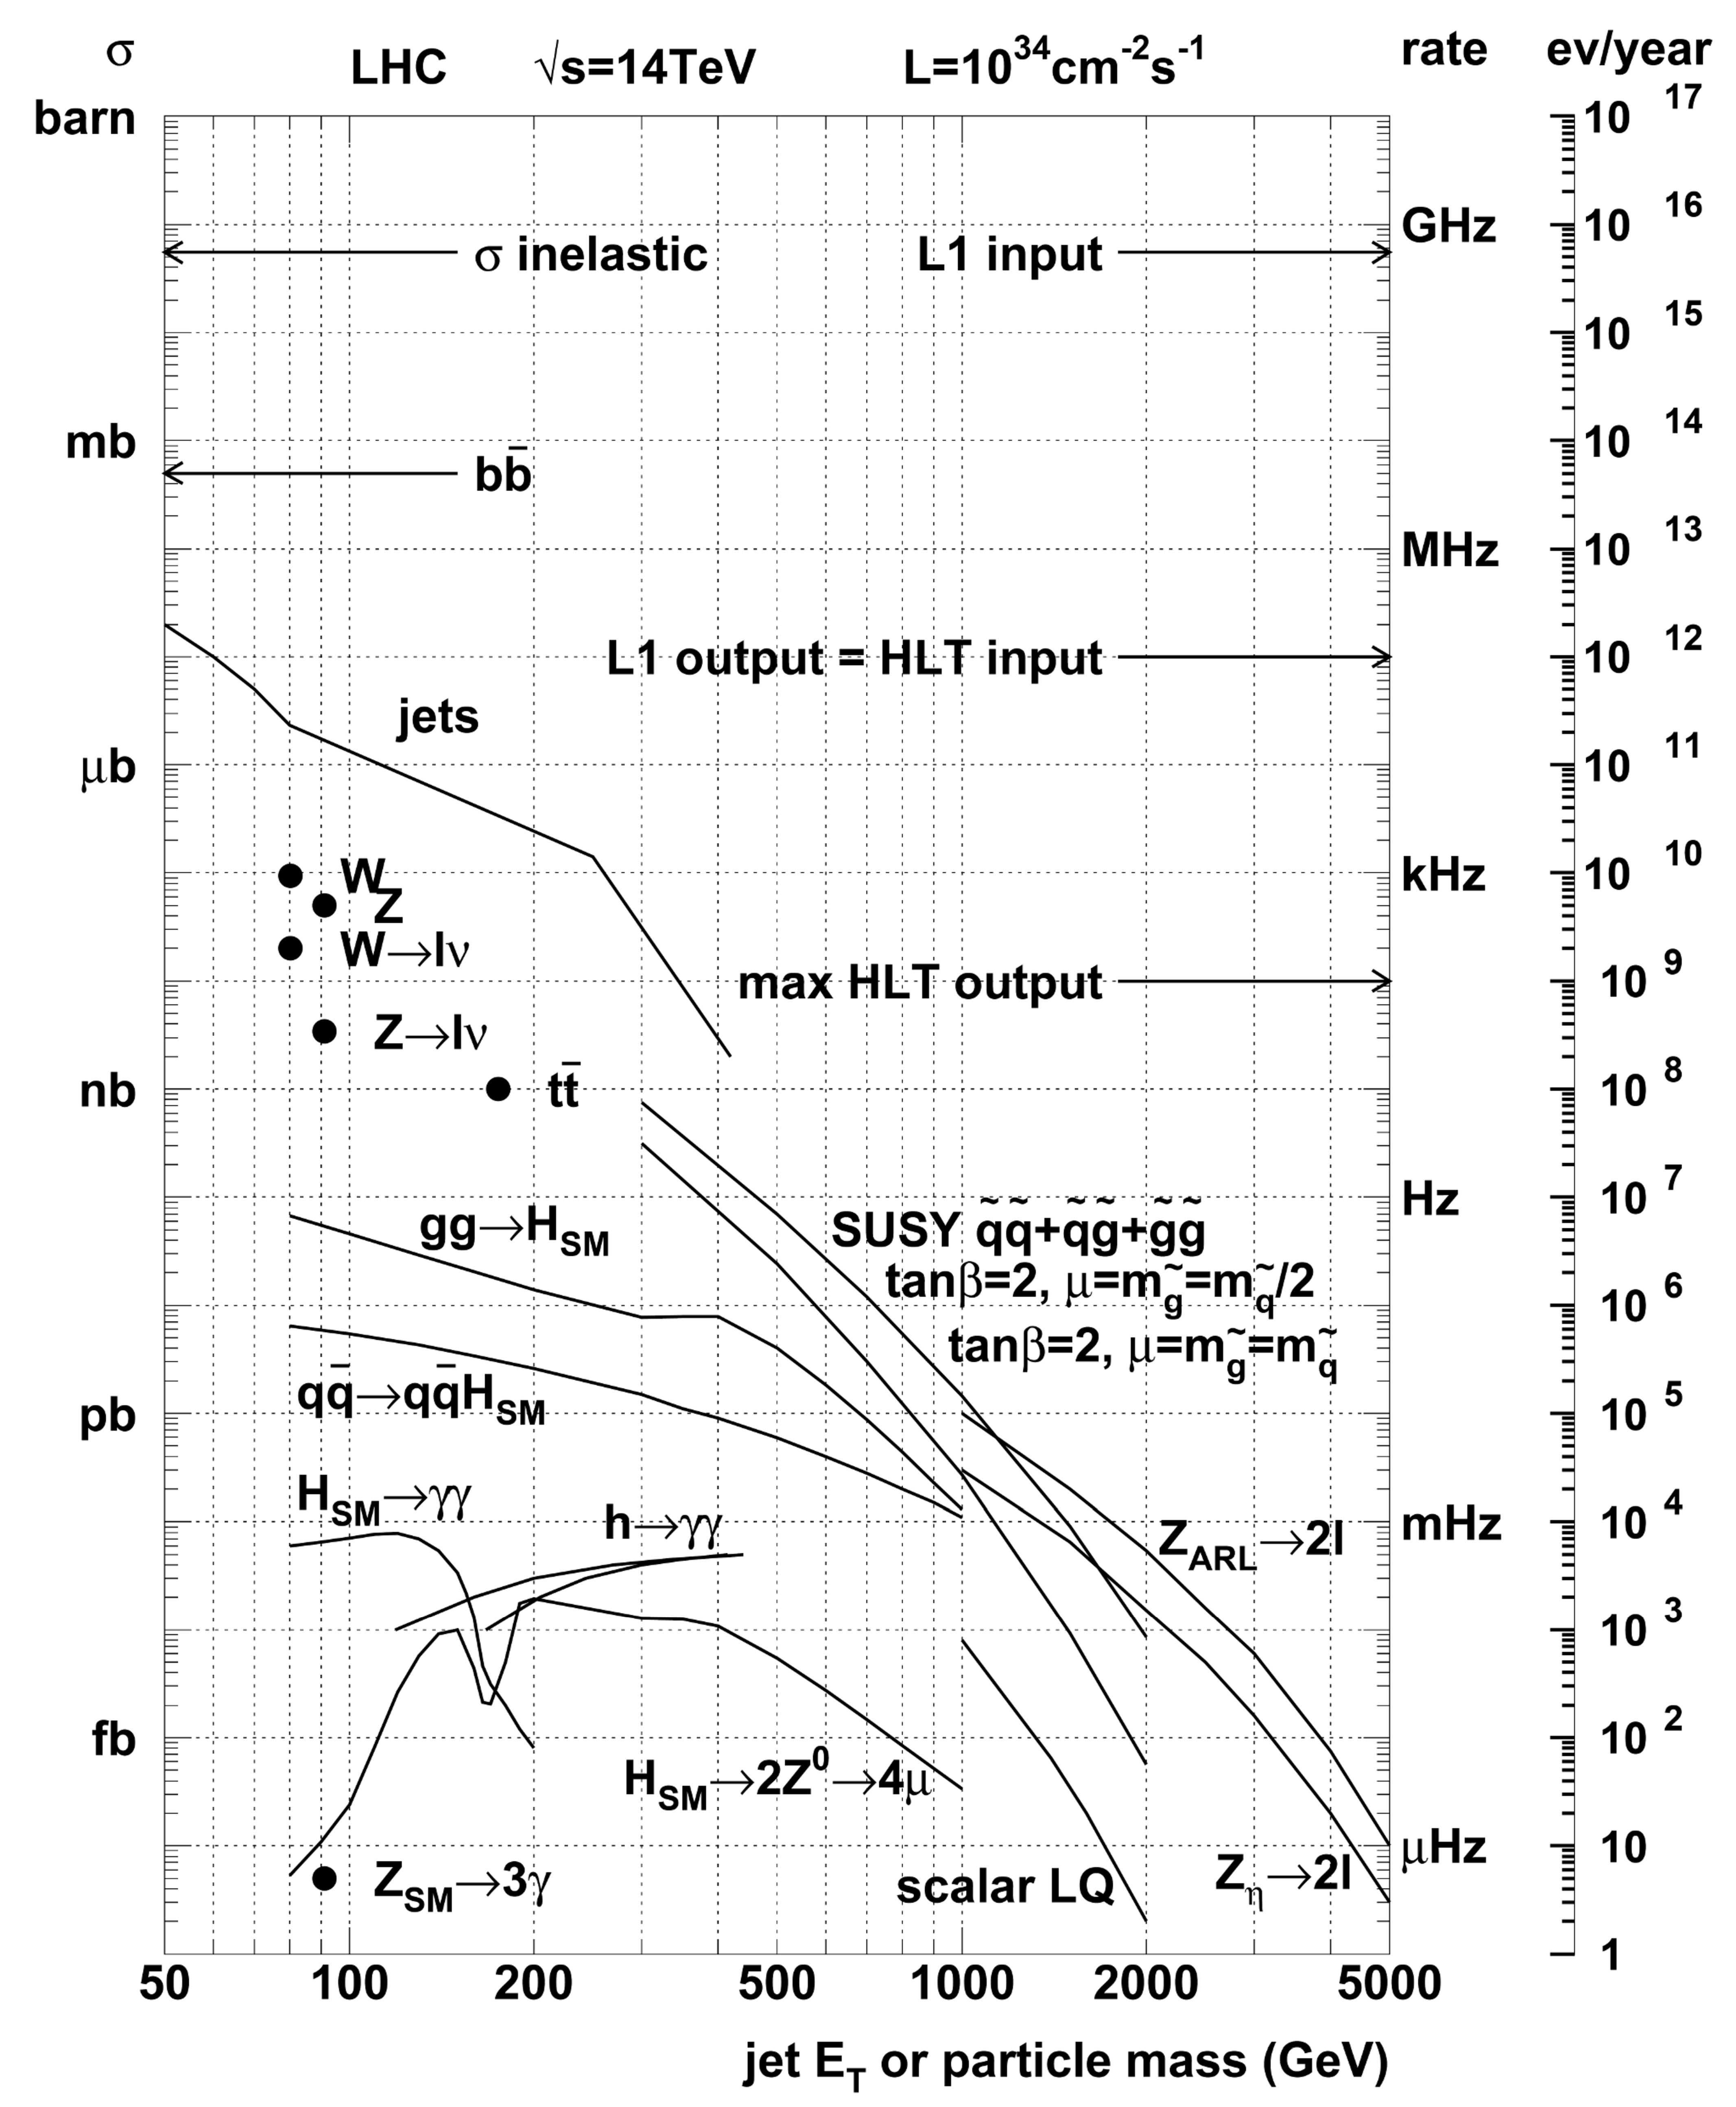
\includegraphics[width=0.55\textwidth]{figs/cms/crossSections.pdf}
\caption{Inclusive proton-proton cross sections for various physics processes, as a function of jet \ET or mass, expected at the LHC at a luminosity of $10^{34}\percms$~\cite{Dasu:2000ge}.}
\label{fig:crossSections}
\end{center}
\end{figure}

Measurements of such processes, as well as precision measurements of SM parameters, require a high interaction rate, and consequently the LHC has a high beam luminosity so that there sufficient statistics available.
Protons are delivered in 2808 bunches per beam, as opposed to a continuous beam, which at design luminosity will separated by 25ns, resulting in an event rate of 40\MHz and an average of 25 inelastic proton-proton interactions, named pile-up (\PU) for each bunch crossing~\cite{Bruning:782076,Ball:2007zza}. 
This high event rate presents the experiments with the data acquisition and readout challenges, whilst retaining excellent signal to background resolution and sufficient radiation hardness in order to withstand the expected fluence.
The primary motivation behind operating the LHC in a heavy-ion mode is to search for evidence of the plasma of quarks and gluons, which is made possible through the resultant production of QCD matter under extreme temperature, density and low momentum fractions of partons~\cite{Baur:687318}.

\section{The Compact Muon Solenoid}\label{sec:cms}
\subsection{Overview}
The Compact Muon Solenoid (CMS)~\cite{oldcms} is a large, general purpose, hermetic particle detector and the smaller of the two multi-purpose experiments operating at the LHC at CERN.
The experiment is divided into a central cylindrical barrel section and two endcap disk sections at each end of the barrel.
A superconducting solenoid encompasses, moving from the interaction point at the centre of the detector outwards, an all silicon tracking detector, a homogeneous lead tungstate ($PbWO_{4}$) electromagnetic calorimeter (ECAL)and hadronic calorimeter (HCAL) comprised of plastic scintillating tiles interspaced with brass absorbers.
Beyond the solenoid there is an outer hadronic calorimeter (HO) and interspaced between the iron return yoke are three different types of Muon Detectors.
There is also a pair of very-forward calorimeters (HF) in the extended rapidity region.

\begin{figure}[htbp]
\begin{center}
\includegraphics[width=0.75\textwidth]{figs/cms/cms_160312_02.pdf}
\caption{Cutaway diagram of CMS’s layers, illustrating its onion-like nature and the location of the detecting technologies within~\cite{Sakuma:2013jqa}.}
\label{fig:cms-cutaway}
\end{center}
\end{figure}

These detectors were designed in order to investigate the wide range of physics phenomena in the LHC's physics program, resulting in the accurate and precise identification and measurement of electrons, photons, jets and muons over both a large energy and momenta range.
Full detector resolution is achieved across $|\eta| < 3.0$, with the hadronic calorimetry having an extended coverage up to $|\eta| < 5.0$ in order to ensure good dijet mass and \MET resolutions.
Sufficient radiation hardness for the expected high fluence and data acquisition and trigger systems required to handle to event rate of the LHC environment had to be considered in the design of the various detectors.

The coordinate system adopted by the CMS experiment has its origin at the nominal interaction point at the centre of the detector. 
The z-axis is parallel to the anti-clockwise proton beam (i.e. towards the Jura mountains from the detector), the x-axis points towards the centre of the LHC, and the y-axis points vertically upwards.
The azimuthal angle, $\phi$, is the angle measured from the x-axis in the x-y plane and the polar angle, $\theta$, is the angle measured from the z-axis.
Pseudorapidity, defined as $\eta \equiv -ln\tan(\theta/2)$, is usually used in lieu of $\theta$ as when the mass considered is negligible $\eta$ converges towards rapidity, defined as $y \equiv 1/2 ln(E+p_{z}/E-p_{Z})$, which is Lorentz invariant along the z-axis.
As such, variables transverse to the z-axis (i.e. the beam line), such as the transverse energy (\ET), momentum (\pT), and missing energy (\MET), depend only on their x and y components.

\subsection{Tracker}\label{subsec:tracker}
The tracker, measuring 5.8m with a 2.5m radius over $|\eta| < 2.5$, surrounds the interaction point, and is designed to provide efficient precision trajectory measurements of charged particles emerging from collisions and precise reconstruction of vertices, whilst operating in a harsh radiation environment (max flux $\approx 10^{7}/s$) and minimising the number charged particles interacting with the tracker (i.e. scattering, producing Bremsstrahlung).
Silicon fulfils these requirements and is used in the inner pixel detector, surrounding the interaction point, and microstrip detector, which encloses the pixel detector, as shown in Fig.~\ref{fig:tracker}.
The high fluence expected closest to the interaction point requires the high granularity pixels provide in order to ensure a low channel occupancy (< 1\%), but the particle flux from $r < 20\cm$ is sufficiently low enough that microstrips can be used without compromising reconstruction efficiency.

\begin{figure}[htbp]
\begin{center}
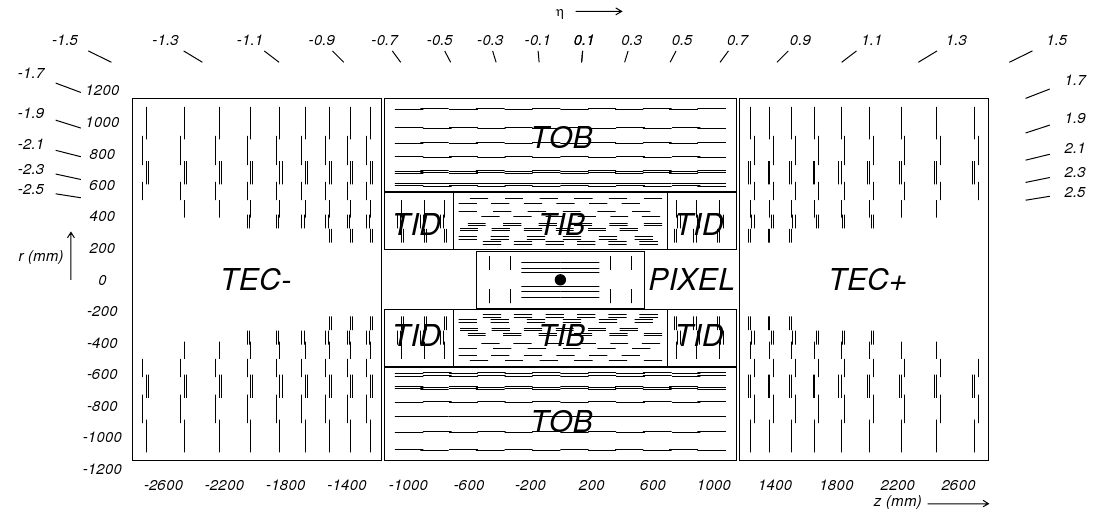
\includegraphics[width=0.97\textwidth]{figs/cms/fig_cmstracker.png}
\caption{Schematic of the CMS tracking detector, displaying the interaction point in the centre and the location the sub-detectors and through the arrangement of the lines, their modules. The double lines present in the microstrip tracker denoting modules with double sided sensors~\cite{Sprenger:2010ss}.}
\label{fig:tracker}
\end{center}
\end{figure}

The tracker system is capable of reconstructing tracks for charged particles of $\pT > 1\GeV$ with an efficiency greater than 99\%, and achieving an impact parameter ($d_{0}$) resolution of $\approx 10\mum$ for $\pT \sim 100\GeV$ charged particles and momentum resolutions between $\sim 1.5\%$ and $\sim 3.0\%$ for $1 < \pT < 100\GeV$ charged particles~\cite{Khachatryan:2010pw,Chatrchyan:2014fea}.

\subsubsection{Silicon Microstrip Tracker}
The silicon microstrip detector is comprised of four parts: the Tracker Inner Barrel (TIB) and Tracker Inner Disks (TID) from $20 < r < 55\cm$, and the Tracker Outer Barrel (TOB) and Tracker EndCaps (TEC) from $55 < r < 116\cm$.
The sensors are rectangular in the barrel region and trapezoid in the endcaps and all consist of singled sided strips of p+-type implants on n-type silicon which are connected to readout chips (ROCs) by aluminium strips.
A total of 9.3 million sensors are used across all four parts, covering an area of 198 $\unit{m}^{2}$.

The TIB provides coverage up to $|z| = 65\cm$ and is comprised of four layers, with the strips having a pitch of 80\mum for the inner two layers and 120\mum for the outer two layers, and a thickness of 320\mum and a typical length of 10\cm across all four layers.
Three disks on each side of the TIB form the TID. 
Each disk is formed of three rings and the sensor pitches across the rings vary between 81-158\mum, but have a thickness of 320\mum throughout.
Surrounding the TIB and TID is the TOB,	which is comprised of six layers which provide coverage up to $|z| = 110\cm$.
In the outer microstrip tracker, increased strip thickness, length and pitch are used in the where the radiation levels are lower so that a similar occupancy and signal to noise ratio to the inner microstrip tracker can be maintained.
The pitch of the strips vary from 183\mum for the inner four layers to 122\mum for the outer two layers, with all having a thickness of 500\mum and a typical length of 25\cm. 
The TEC's nine disks per endcap extend coverage from $|z| = 120\cm$ to $|z| = 280\cm$, with the number of rings per disk varing from four to seven depending on the disk's position in z.
The thickness of the sensors in the TEC are 320\mum and 500\mum in the three innermost rings and the rest respectively.
A number of ``stereo'' modules of two back to back sensors are used in the inner two layers of the TIB and TOB, the inner two rings of the TID and the inner two and the fifth rings of the TEC.
These sensors are aligned at an angle of 100 mrad to each other, allowing measurements of both the $r-\phi$ and r-z coordinates, to a point resolution of 23-34\mum $r-\phi$ and 23\mum in z and 35–52\mum r-phi and 52\mum in z in the TIB and TOB respectively.

\subsubsection{Silicon Pixel Tracker}
The original ``Phase-0'' silicon pixel detector was comprised of three 53.3\cm long barrel layers at mean radii of 4.4, 7.3 and 10.2\cm and two endcap disks either side of the barrel at $|z| = 34.5$ and 46.5\cm that extend from $r = 6.0$ to 15\cm.
The pixel sensors consist of n+-type implants  on n-type silicon which are connected by indium bump-bonds to highly integrated ROCs.
Each of the 66 million pixels measures $100 \times 150\mum^{2}$, covering a total surface area of 1.06 m$^{2}$, with point resolutions of 10\mum in $r-\phi$ and 20\mum in z, which provides the granularity required to have a high track reconstruction efficiency and to be able to precisely calculate the track impact parameters and vertex position.

\editComment{Check rewording of this long sentence to make two shorter ones after receiving Jo's feedback}
The original pixel detector was designed to operate a nominal instantaneous luminosity of $1 \times 10^{34}\percms$, however, with the ``Phase-I'' LHC conditions of increased \PU from running at a higher instantaneous luminosity with the same 25\ns bunch spacing, the detector will suffer track reconstruction efficiency degradation due to radiation damage.
Therefore during the End of Year Technical Stop that took place between data taking in 2016 and 2017, the pixel detector was completely replaced.
A more detailed description of the Phase-I Pixel detector can be found in~\cite{CMS:2012sda}, given that none of the results discussed in~\ref{sec:results} involve data collected after 2016.
%%Like the original pixel detector, the Phase-I detector's 124 million pixels also measure $100 \times 150\mum^{2}$ (covering a total surface area of 1.95 $m^{2}$) and the sensors are also n+-type implants on n-type silicon.
%%The Phase-I Pixel detector is comprised of four 54.9\cm long barrel layers at mean radii of 3.0, 6.8, 10.9 and 16.0\cm and three endcap disks at each end of the barrel at $|z| = 29.1, 39.6 and 51.6\cm$ that extend from $r = 4.5 to 16.1\cm$.

\subsection{Electromagnetic Calorimeter}\label{subsec:ECAL}
Beyond the tracker, the ECAL~\cite{CMS:1997ysd,CMS:2002xia}, a homogeneous calorimeter, measures the energies of electrons and photons using lead tungstate scintillating crystals. 
The choice of using lead tungstate crystals was based on the needs of both having a compact detector which could fit with the HCAL inside the solenoid and containing the showers' energy within this calorimeter, which were met with its short radiation length (0.89\cm) and small Molier\'{e} radius (2.2\cm).

61,200 crystals are mounted in the barrel, with 7,324 crystals for each endcap.
As the crystals only emit a small amount of scintillation light when the electromagnetic shower de-excites, the photodetectors used to amplify the light must be able to operate within the solenoid's field and and withstand the high radiation environment.
Avalanche photosdiodes and the more radiation hard vacuum photodiodes are used in the barrel and endcap regions respectively to convert the light into an electrical current that is directly proportional to the energy of the induced electromagnetic showers.
The emitted light emitted by these crystals is short, well defined and fast, with 80\% collected within one 25\ns bunch crossing, with the signals being digitised on-detector and buffered until a Level-1 Trigger decision has been made.

The barrel and endcap cystal systems are supplemented by a Preshower (ES)~\cite{Loos:539819} device, located in front of the ECAL endcaps, for discrimination between neutral pions and photons within the fidicial region $1.653 < |\eta| < 2.6$.
For each ES, two lead radiators initiate the electromagnetic showers and two silicon strip sensors, orthogonal to one another to provide fine resolution, are placed after the radiators measure the energy deposited.
The thickness of the radiators was chosen to ensure ~95\% of incident photons shower before reaching the second silicon strip sensor, namely two and one radiation lengths for the first and second lead radiators respectively.

\begin{figure}[htbp]
\begin{center}
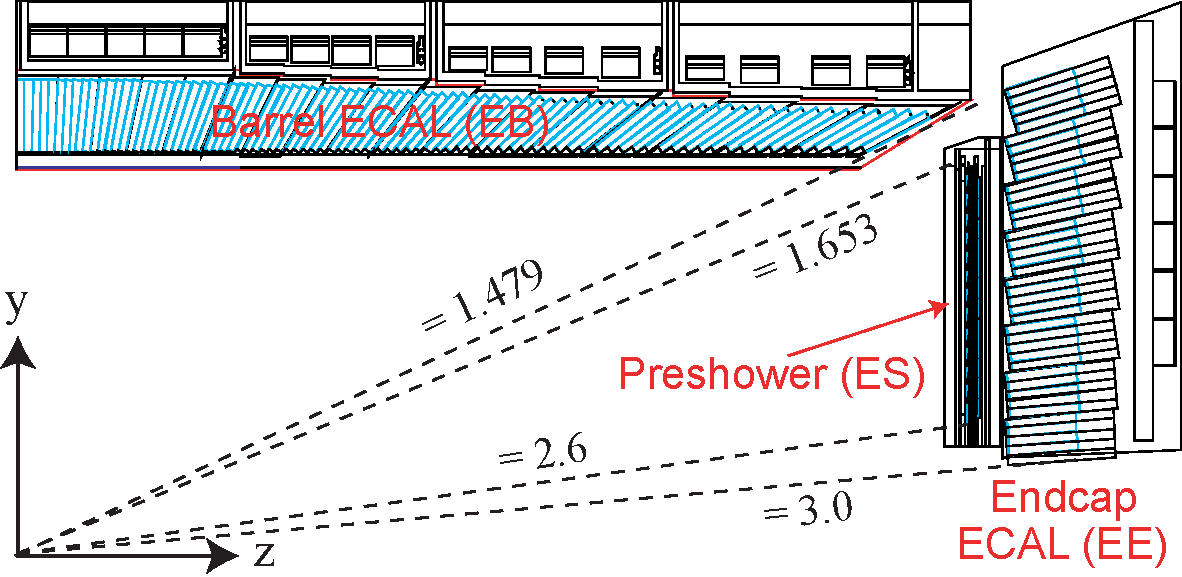
\includegraphics[width=0.97\textwidth]{figs/cms/ECAL_Transverse_section.pdf}
\caption{Layout of one quadrant of the ECAL system, illustrating locations of the various subsystems~\cite{Bayatian:2006nff}.}
\label{fig:ecal}
\end{center}
\end{figure}

Electron test beam measurements without a magnetic field and without material between the test beam and ECAL have determined the energy resolution, $\sigma_{E}$, to be,

\begin{equation}
(\frac{\sigma_{E}}{E})^{2} = (\frac{2.8\%}{\sqrt{E}})^{2} + (\frac{12\%}{E})^{2} + (0.3\%)^{2} \;.
\label{eq:ecalResolution}
\end{equation}

where E is the energy of the incident particle in \GeV, the first term representing the statistical fluctuations in the amount of photo-electrons produced, the second denoting noise from the electronics ad digitisation, and the third term covering any non-uniform longitudinal response and shower containment losses~\cite{Adzic:2007mi}.

\subsection{Hadronic Calorimeter}\label{subsec:HCAL}
Hadronic particles penetrate through the ECAL into the HCAL~\cite{CMS:1997xji}, where hadronic jets have their energies measured and are contained for determination of the missing transverse energy and protection of the muon detectors~\cite{HCAL:tdr}.
As such, the HCAL was designed to have as much absorber material within the solenoid coil as practical. 
The barrel (HB) and and endcap (HE) both use plastic scintillator tiles interspersed between brass and steel absorber plates, with the latter being used for the external plates for structural strengthening.
Wavelength shifting fibres embedded in the tiles converts the scintillated light and channels it to hybrid photodiodes.
%%%
The HB covers the rapidity range $|\eta| < 1.4$, with the HE overlapping it and providing coverage over the range $1.3 < |\eta| < 3.0$, with each being segmented in $\eta - \phi$ by $0.087 \times 0.087$ for $| \eta | < 1.6$ and up to $0.17 \times 0.17$ for $| \eta | >= 1.6$.

Due to space constraints within the solenoid, the HB cannot fully contain hadronic showers and as such is supplemented by an additional calorimeter in the barrel region outside the coil (HO). Given the outer hadronic calorimeter's limited size and function, it will not be discussed further here, but a thorough description of the HO can be found in~\cite{HO}.

The forward calorimeters (HF)~\cite{HF} overlap with the HE and cover the $2.9 < \eta < 5.0$ rapidity region.
As the forward region experiences the most severe radiation environment, the technology used must be able to withstand such large radiation doses~($10^{9}$ rad). 
Interspaced between steel absorbers, quartz fibres are used produce Cherenkov light due to their radiation hardness, fast response time, production of Cherenkov radiation above a certain energy threshold (thus ignoring low energy particles), and ability to give directional information due to the light being strongly correlated with the showers' trajectories.
The Cherenkov light produced is transmitted down the fibres to individually shielded photomultiplier tubes contained in readout boxes.

Using test beams of electrons, muons and pions, the combined energy resolution of the ECAL and HCAL together was determined to be, 

\begin{equation}
(\frac{\sigma_{E}}{E})^{2} = (\frac{84.4 \pm 1.6\%}{\sqrt{E}})^{2} + (7.4 \pm 0.8\%)^{2} \;.
\label{eq:hcalResolution}
\end{equation}
for the HB and HE ~\cite{Abdullin:2008zzb}, and,

\begin{equation}
(\frac{\sigma_{E}}{E})^{2} = (\frac{198\%}{\sqrt{E}})^{2} + (9\%)^{2} \;.
\label{eq:hfResolution}
\end{equation}

for the HF~\cite{Bayatian:2006jz}.

\subsection{The Superconducting Solenoid}\label{subsec:magnet}
One of the defining features of the CMS detector is the superconducting solenoid which encompasses the silicon tracker and calorimetry~\cite{Acquistapace:1997fm,Herve:2000}.
The 220T cylindrical coil measures 13m long, has a 5.9m inner diameter, is situated inside a vacuum tank where it is cooled to its operation temperature by liquid helium to 4.5K, and operates at magnetic field of 3.8 Tesla\footnote{Whilst the solenoid was designed to operate at 4T, the CMS collaboration chose to operate it at 3.8T in order maximise the lifetime of the apparatus}.
The large bending power within the solenoid not only provides excellent momentum resolution for charged particles within the tracking detector, but it also prevents low transverse momentum charged particles from reaching the calorimetry and negatively impacting on energy resolution and isolation efficiency.
An iron return yoke guides and contains the return magnet field, which is sufficiently strong ($\approx$ 1.7T in the barrel and outermost endcap disk) enough to enable accurate momentum resolution for tracking and charge identification of high momentum ($\approx$ 1\TeVc) muons.

\begin{figure}[htbp]
\begin{center}
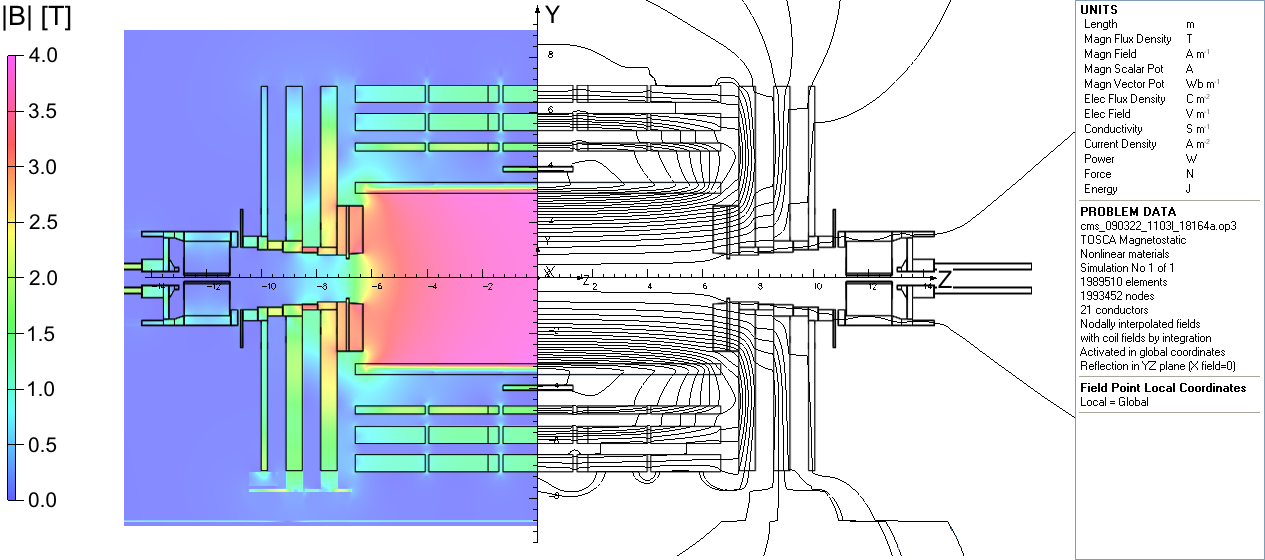
\includegraphics[width=0.97\textwidth]{figs/cms/cms_magnetic_field.png}
\caption{Longitudinal section of the CMS detector, illustrating the predicted magnetic field strength (left) and field lines (right) for the operational central magnetic flux density of 3.8T~\cite{Chatrchyan:2009si}.}
\label{fig:magneticField}
\end{center}
\end{figure}

\subsection{Muon Detectors}\label{subsec:muon chambers}
Detecting muons is incredibly important for CMS (as implied by the experiment’s name), given many of the signatures of interesting events involve them, including those from SUSY models and the so called “gold-plated” SM Higgs decay into a pair of $Z^{0}$ bosons, which in turn decay into four muons. 
Being Minimum Ionising Particles (MIPs), muons pass through the detector and the magnet with minimal interaction.
Consequently, the muon chambers~\cite{CMS:1997iti} are placed outside the solenoid and provide a strong clean signals which can be triggered upon.

Given that the magnetic field outside the solenoid is non-uniform and the radiation environment varies, differing detector technologies are used in order to provide a high performance system which delivers the fast identification and momentum resolution required. 
Interspaced between the iron return yoke rings and disks are three gaseous detector technologies: Drift Tubes (DTs), Cathode Strip Chambers (CSCs) and Resistive Plate Chambers (RPCs).

\begin{figure}[htbp]
\begin{center}
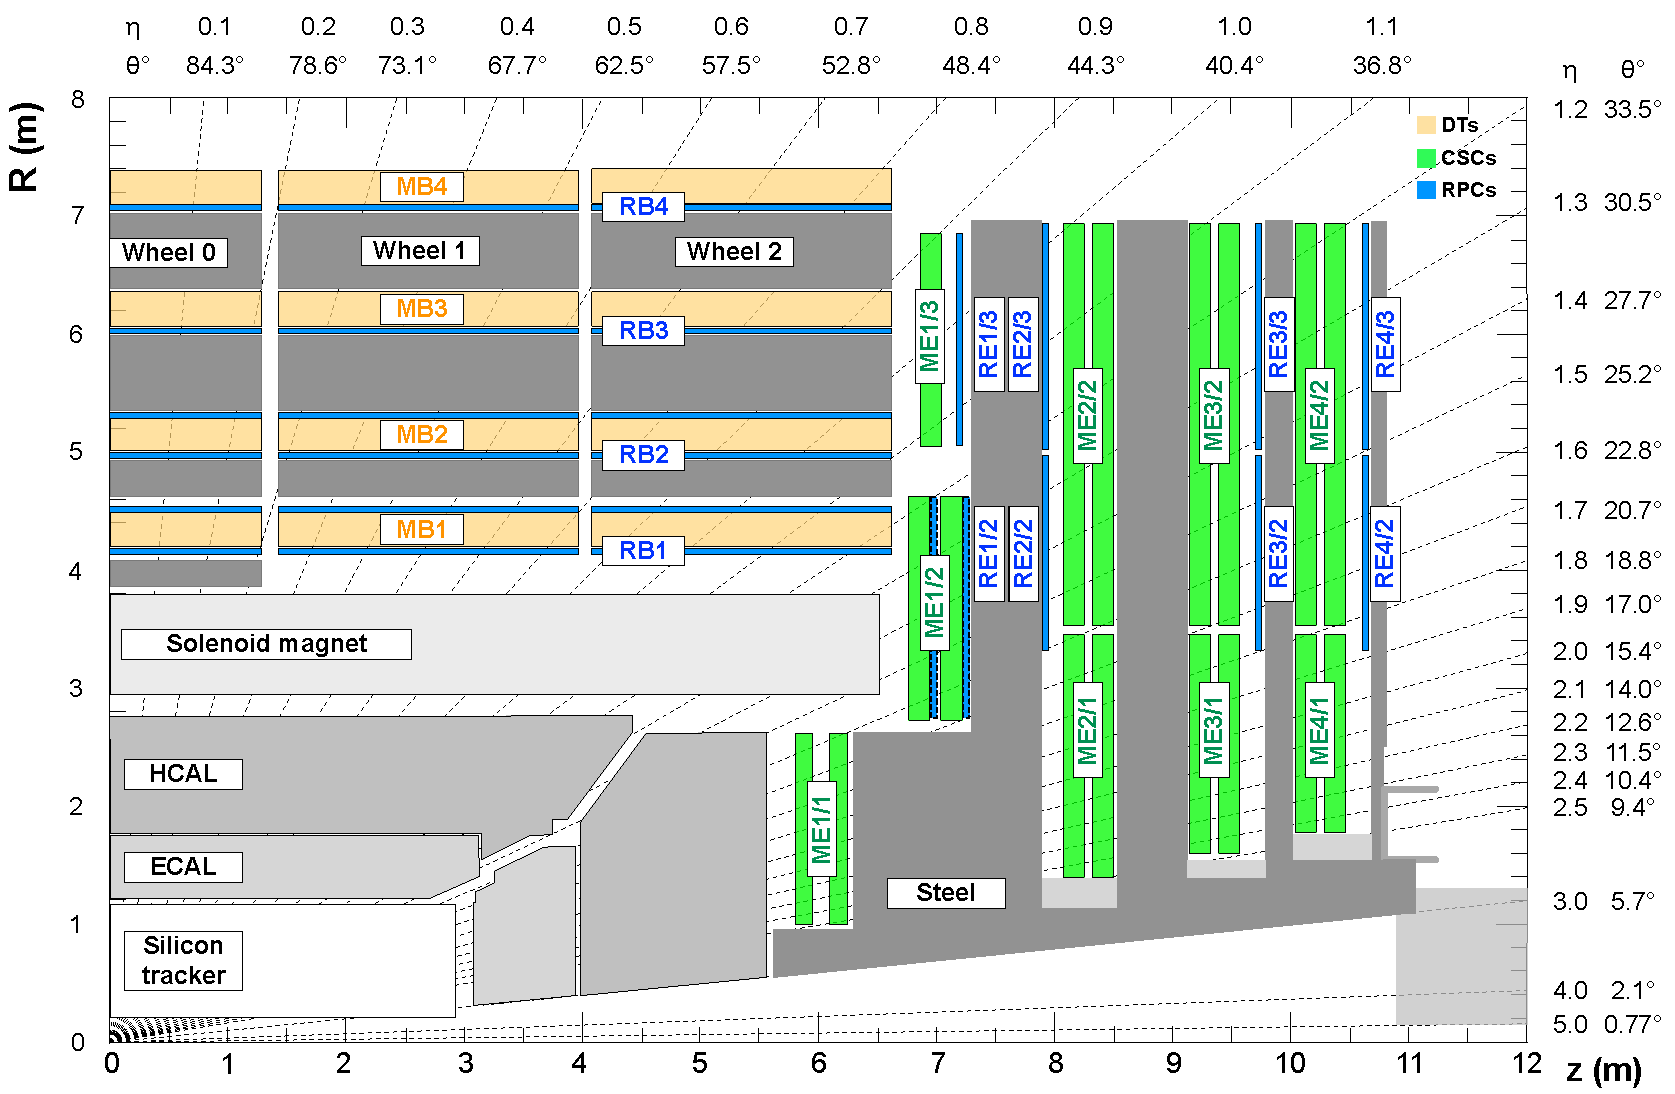
\includegraphics[width=0.97\textwidth]{figs/cms/cms_muon_quadrant_run_ii.pdf}
\caption{Layout of one quadrant in r-z of the CMS Muon Detectors in their Run II configuration (from 2015), which saw the addition of CSC and RPC disks ME 4/2 and RE 4 respectively~\cite{CMS-DP-2016-046}.}
\label{fig:muonChambers}
\end{center}
\end{figure}

The DTs operate in the barrel region across $|\eta| < 1.2$, where the magnetic field strength is low as most of the return field is contained in the iron yoke,	and each tube is $4.2\cm x 1.3\cm$ cell filled with an Ar/$CO_{2}$ mixture of 85\%/15\%.
The DT chambers are organised into four stations of cylindrical layers and for each station, the chambers are subdivided into three ``superlayers'' (/SLs).
Each SL is comprised of four layers of DTs, where the outer SLs measure coordinates in the $r-\phi$ plane and the inner SL measures in the r-z plane (which the outermost station lacks), which provides point resolutions of $\approx 200\mum$ and a $\phi$ directional precision of $\approx 1$ mrad.

CSCs are employed in the endcaps across $0.9 < \eta < 2.4$ , where the mangetic field is non-uniform and there is a higher rate of muons than in the barrel, and are organised into four stations of concentric disks.
Initially only the inner ring of the outermost (fourth ) disk was installed, with the outer ring (ME4/2, see Fig.~\ref{fig:muonChambers}) being installed in the Long Shutdown 1 (LS1) of the LHC during 2013-2015~\cite{Battilana:2017mrm}.
Each CSC is composed of six gas gaps, with six planes of anode wires running almost perpendicularly to six planes of cathode strips, and thus provides six position measurements per chamber with a precision in the $r-\phi$ plane of 75\mum for the first station and 150\mum for the other stations\cite{CMS:1997iti}.

RPCs provide coverage over $|\eta| < 1.8$, which originally only extended to $|\eta| < 1.6$, instead of the planned $|\eta| < 2.1$, for financial reasons. 
During LS1, a fourth endcap disk with RPCs was installed which extended coverage to the current coverage of $|\eta| < 1.8$\cite{Battilana:2017mrm}.
Although the RPCs have a coarser position resolution ($\approx 1\cm$) than the DTs and CPCs, they have fast response times and excellent time resolution ($\approx 2\ns$).
As such, RPCs provide additional but complimentary input to trigger decisions.
A RPC is formed of two parallel resistive plates, separated by a few millimetres, with a large electric field applied across the gas filled gap.
The barrel contains six layers of RPCs, two layers in the first two stations and one in each of the outer stations, and the endcaps have 4 RPC disks each, one for each CSC station.

Collectively with information from the tracking system to improve performance (as described in Chapter~\ref{chapter:data-mc}), these systems provide a momentum resolution of $1.3\% to 2.0\%$ and up to $\approx 6\%$ in the barrels and endcaps respectively and a charge misidentification rate of $< 0.1\%$ for muons with $\pT < 100 \GeV$~\cite{Chatrchyan:2012xi,Chatrchyan:2013sba}.

\subsection{Trigger and Data Acquisition Systems}\label{subsec:trigger}
At design luminosity, the LHC has a bunch crossing (BX) rate of $40\MHz$, i.e. $\approx~10^{9}$ inelastic events per second, with each proton-proton collision event having a size of $\approx 1.5MB$~\cite{Bayatian:2006nff}.
Since is is not possible to store every event or to have sufficient bandwidth to read all events off the detector, the CMS trigger system~\cite{Dasu:2000ge,Sphicas:2002gg} has to drastically reduce the data rate to the manageable level of $\approx 1\kHz$\footnote{Since initial operations, the original event storage rate of 100\Hz has been increased to 0.5 to 1\kHz}~\cite{Dasu:2000ge,phase1L1TDR}.

The vast majority of events are uninteresting from a physics perspective, with the cross sections of interesting processes being at least $\approx 10^{7}$ smaller than the total proton-proton cross section of $110.6 \pm 3.4$ mb~\cite{Antchev:2017dia}.
Therefore the CMS trigger system is designed to reject these background events and select events in a manner that allows all possible new physics signatures to be detected whilst keeping acceptance thresholds sufficiently as low as reasonably possible, within the constraints of the design readout and storage capacity.
The CMS trigger system is comprised of two stages, The Level-1 (L1) Trigger and the High Level Trigger (HLT), as it not feasible to reduce the data rate in a single processing stage without compromising on physics performance.

\subsubsection{L-1 Trigger}\label{paragraph:L1}
The Level-1 Trigger reduces the raw $40\MHz$ rate to $\approx100\kHz$ and consists of FPGAs (Field Programmable Gate Arrays) and ASICs (Application Specific Integrated Circuits), which have to identify hard scattering physics signals at a high efficiency with acceptance thresholds as low as possible, within constraint of the system having to analyse every bunch crossing (BX).
The strict time limitations on how long it takes for the data can be collected and read out, precludes both the reading out of events in full and of the use of iterative reconstruction algorithms.
As the selection cannot be done before the subsequent BX, given the above constraints, the L1 Trigger uses a pipelined approach which provides a total system latency of $\approx$ 3.8\mus, during which the detector data is buffered (the Tracker and ES buffers being the limiting factor of the system latency) prior to either being read out or discarded.
The L1 acceptance decision is based on whether \emph{trigger primitives} formed from promptly available data from the ECAL, HCAL or muon detectors above the pre-determined \pT or \ET thresholds, with the highest ranked candidates being forwarded from the global calorimeter and global muon triggers to the Global Trigger, which either rejects an event or accepts it for further evaluation by the second stage, the HLT.
Tracking information is not used in the L1 Trigger as its inclusion was determined to be unnecessary for nominal LHC conditions, and consequently, it has not been designed to be read out for every event.

Given that following LS1 it was planned that both the instantaneous luminosity and centre-of-mass energy of the LHC were to increase, the Phase-I Trigger Upgrade~\cite{Tapper:2013yva} was undertaken in order to prevent the physics program being compromised from a substantial increase in the trigger thresholds that would be required to maintain the 100\kHz L1 trigger limit.	

The Phase-I Calorimeter Trigger Upgrade is based on a \emph{time-multiplexed} architecture which uses large FPGAs on a small number of general-purpose boards with fast optical links that allow for full granularity data to be used.
This \emph{time-multiplexed} trigger concept differs from the previous traditional regional reconstruction data reduction architecture, which forwards the best candidates at each regional level to the next stage which covers a larger region of the detector, by processing all data for every \emph{n}th bunch crossing on one of \emph{n} identical processors.
Such a system requires at least two layers, linked by a switching network which buffers and transmits data from the multiple sources to a single processor, as illustrated in Fig.~\ref{fig:TMT}.

\begin{figure}[htbp]
\begin{center}
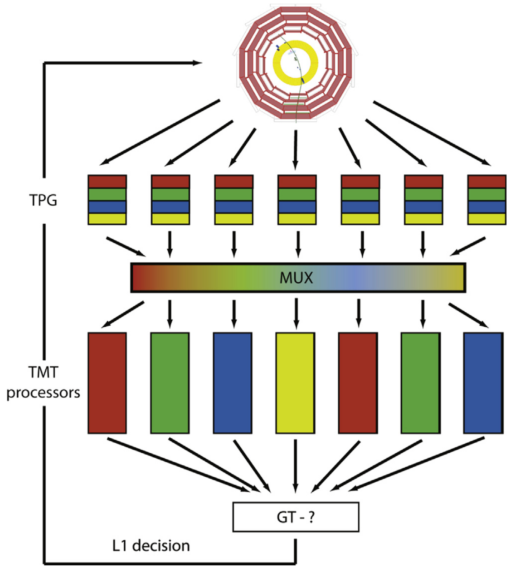
\includegraphics[width=0.97\textwidth]{figs/cms/TMT.pdf}
\caption{In a time-multiplexed trigger, all data from the Trigger Primitive Generators (TPG) covering the entire detector are transmitted to one of ``n'' identical processors after passing through the multiplexing fabric (MUX), a serial interconnection linking each TPG to each TMT processor, before being passed to the Global Trigger (GT) where the decision of whether or not to issue a L1 receipt to the HLT is determined~\cite{tmttelba}.}
\label{fig:TMT}
\end{center}
\end{figure}

Advantages of a time-multiplexed architecture include:
\begin{itemize}
\item minimised boundary issues and data sharing between processors, saving time and resources and allowing for data from the entire calorimeter for a bunch crossing to be considered on a single processor and thus consider candidates that would have been discarded by the previous regional triggers.
\item synchronisation being only required within each processor instead of the entire system.
\item system demonstration with a single processor as each processor is identical and fully pipelined (no sideways connections).
\item validation only requiring one processor as each is identical and has no sideways communication.
\item the loss of a processor resulting in the loss of a bunch crossing instead of a region of the detector.
\item the use of spare processors to test new algorithms online in parallel with the nominal trigger without affecting the current system and as backup processors in case of the failure of another.
\end{itemize} 

The electronics of the Phase-I Trigger were installed during LS1 and ran using the legacy trigger system during 2015 with the new trigger system (Fig.~\ref{fig:trigger}) running in parallel for validation prior to commissioning and usage during 2016~\cite{Zabi:2017lya}.

\begin{figure}[htbp]
\begin{center}
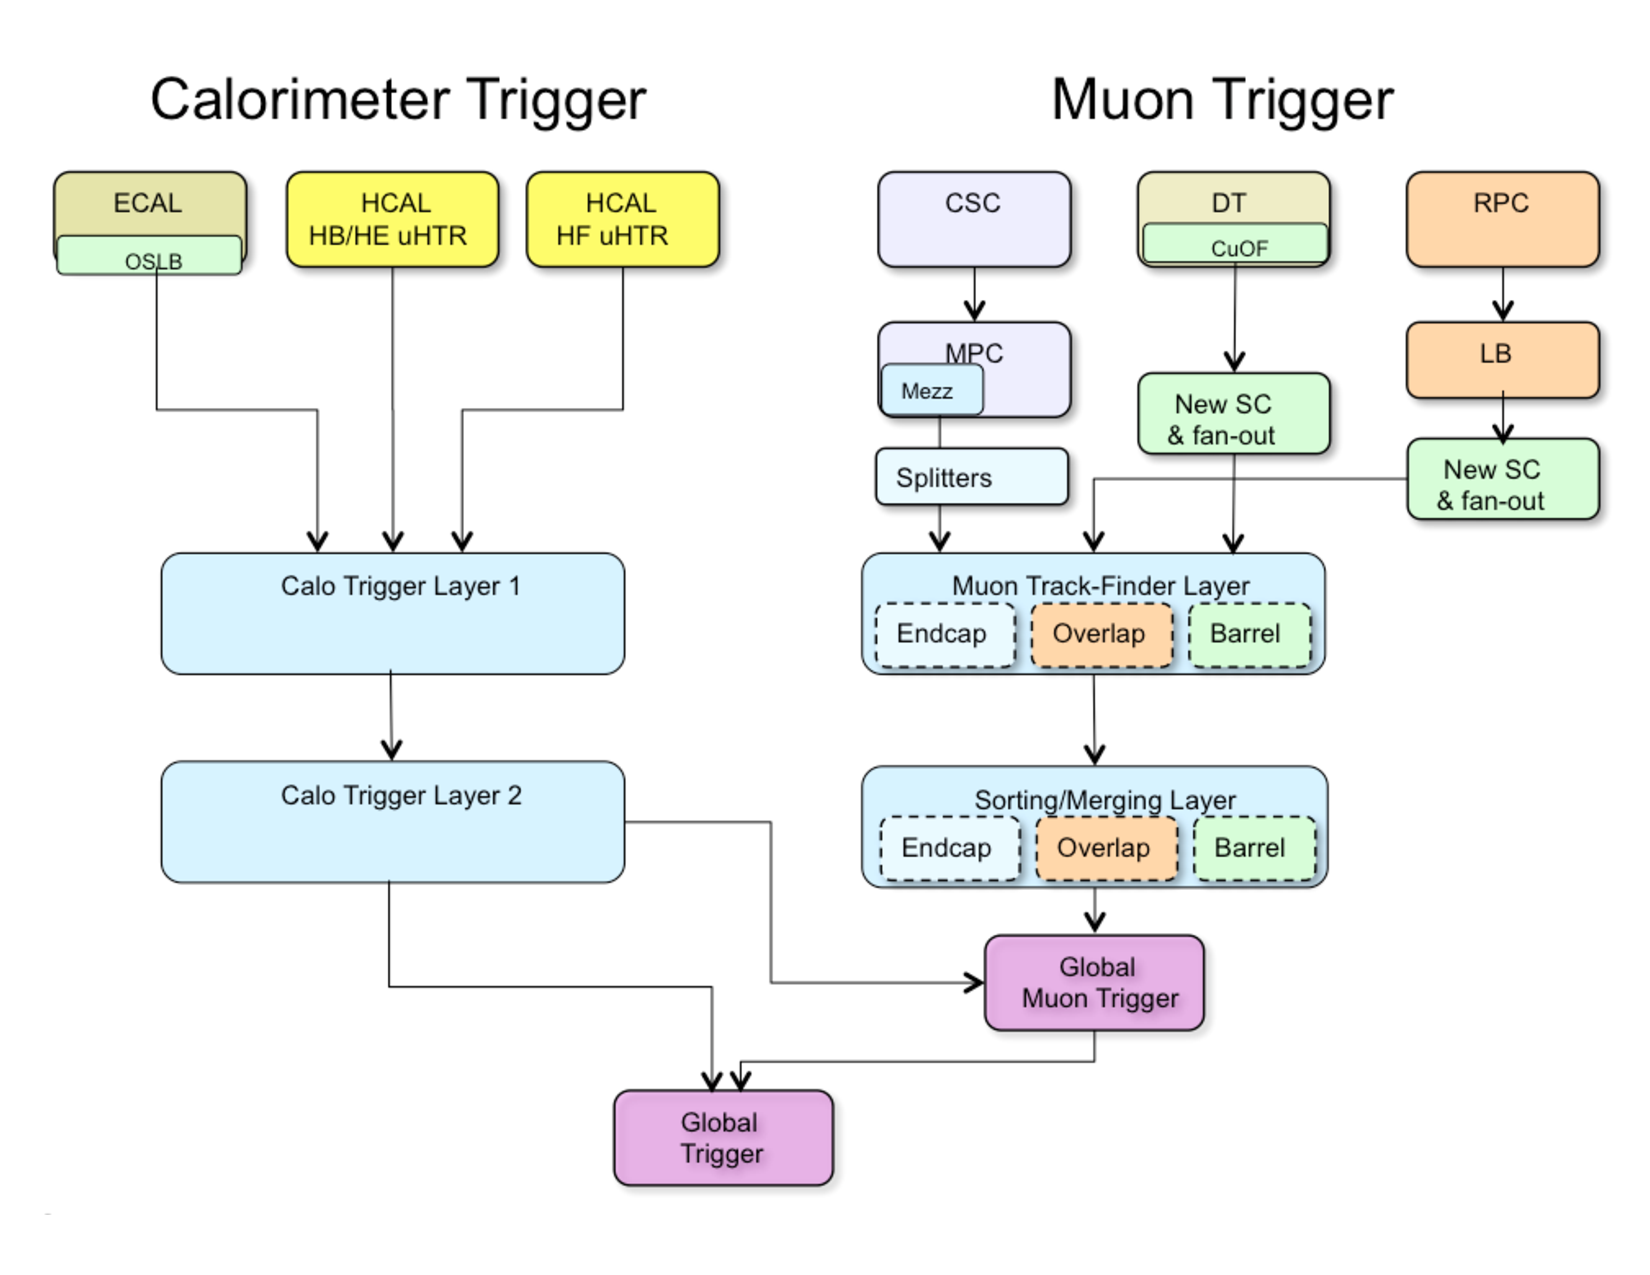
\includegraphics[width=0.97\textwidth]{figs/cms/TrigUpgradeBlockDiagram.pdf}
\caption{Current (Phase-I) Level-1 Trigger Architecture~\cite{Tapper:2013yva}.}
\label{fig:trigger}
\end{center}
\end{figure}

The success of this architecture has motivated a similar time-multiplexed approach for a potential track finding system for the Phase-II Outer Tracker, as discussed in~\ref{sec:TMTT}.

\subsubsection{High Level Trigger and Data Acquisiation}\label{paragraph:HLT}
Upon receipt of a L-1 trigger, the Data Acquisition (DAQ) system (Fig.~\ref{fig:DAQ}) reads out the buffered data from the detector Front-End Drivers, buffers it in the Readout Systems until the Builder Network (controlled by the Event Manager) can transfer data to the Filter Systems where the event fragments are collated into a complete event and processed through the HLT algorithms~\cite{Sphicas:2002gg}. 

\begin{figure}[htbp]
\begin{center}
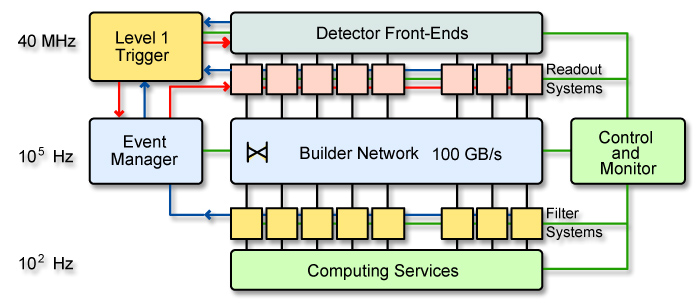
\includegraphics[width=0.97\textwidth]{figs/cms/CMS_DAQ.jpg}
\caption{Overview of the CMS Data Acquisition system architecture~\cite{Sphicas:2002gg}.}
\label{fig:DAQ}
\end{center}
\end{figure}

The HLT reduces the L1 rate of $\approx 100\kHz$ to the output rate of $\approx 1\kHz$.
In contrast to the L1 trigger, the HLT algorithms are performed by commercially available processors by the CMS Software (\CMSSW), which allows for great flexibility of alogirthms and the use of the full detector readout (including the Tracker and ES) to reconstruct the event and select events.
Given that the the time limitations on the HLT are not as strict as the L1 Trigger, with events requiring an average of $\approx 40\ms$, more sophisticated reconstruction and selection algorithms are used.
This however, does not mean that the full event is reconstructed, as such a task is too CPU intensive to be done online within the latency constraints.
The output from the Filter System is collected by the Computing Services and forwarded to the offline Tier-0 computing centre for offline processing and reconstruction and to the detector's online monitoring systems.


\chapter{Monte Carlo studies for a Track Finding Processor at the High Luminosity-LHC}\label{chapter:tk-upgrade}
As the statistical gains for an experiment that is operated at a constant luminosity increasingly diminish over time, it is planned to preserve and extend the LHC's physics discovery potential by operating the LHC with an increased instantaneous luminosity.
Before the start of these higher luminosity operations, the then life-expired CMS tracker will need replacing.
The new tracker will not only need to have increased radiation hardness to withstand the increased \PU environment, but also the capability to provide limited tracking information to the L-1 trigger in order to keep the L-1 acceptance rate below 750\kHz.

This chapter introduces the motivations behind the high luminosity upgrade of the LHC, the planned upgrade of the CMS tracker and the studies undertaken for one of the proposed track finding systems for the upgrade tracker.

\section{The High-Luminosity Large Hadron Collider} \label{sec:hl-lhc}
In order to fully exploit the physics discovery potential of the LHC, it is planned to increase the instantaneous luminosity the accelerator can deliver by up to an order of magnitude greater than the nominal design.

The High-Luminosity Large Hadron Collider (HL-HLC) upgrade is intended to increase the instantaneous luminosity of the LHC up  to $7.5 \times {10}^{34}$\percms.
This corresponds to an average number of proton-proton interactions (\PU) per 40\MHz bunch crossing of between 140 and 200 and a total integrated luminosity of up to of 3000\fbinv being provided to both the ATLAS and CMS experiments during the 10 year planned lifetime of the HL-LHC.

The installation of the HL-HLC upgrade is planned to take occur during Long Shutdown 3, which is currently expected to start during 2024~\cite{ApollinariG.:2017ojx}. 
The timing of LS3 is motivated in part by the need to replace the inner triplet quadrupole magnets that focus the beams at the ATLAS and CMS collision regions are expected to be near life-expired due to radiation exposure~\cite{hl-lhc-prelim-design-report,CMSCollaboration:2015zni}.

The instantaneous luminosity, $L$, of an accelerator and its beam parameters are related by~\cite{ApollinariG.:2017ojx}: 

\begin{equation}
L \propto \frac{n_{b}N^{2}_{p}}{\beta^{*}} R  \;
\label{eq:machineLumi}
\end{equation}

where $n_{b}$ is the number of bunches, $N^{2}_{p}$ is the number of protons per bunch, $\beta^{*}$ is the focal length (beam $\beta$ value) at the collision point, and $R$ is a crossing-angle-dependent luminosity geometrical reduction factor, .

As it is not practical to increase the number of proton bunches due to the resultant heat loads induced by electron clouds, the increase in the machine's luminosity will be achieved by increasing the number of protons per bunch and by reducing $\beta^{*}$~\cite{ApollinariG.:2017ojx}.
Replacing Linac2 with the new Linear accelerator 4 (Linac4)~\cite{linac4} during the Long Shutdown 2 (2019-2020) will allow for the number of protons per bunch to be increased by a factor of two compared to the nominal LHC design (and to increase the injection energy by a factor of three).
The new, more radiation tolerant, quadrupole magnets to be installed during LS3 will provide the higher magnetic field strength and the aperture needed to provide the lower $\beta^{*}$ required to increase the instantaneous luminosity. 

\section{The Phase-II Outer Tracker Upgrade}\label{sec:tk-upgrade}
To meet the significant challenges of, and exploit, the increased instantaneous luminosity delivered by the HL-LHC, the CMS detector will be substantially upgraded.
This upgrade will take place during LS3 and will not only deliver the improved radiation hardness to handle the increase in radiation from the increased \PU but also greater detector granularity to reduce occupancy and enhanced bandwidth and triggering capabilities to avoid compromising physics potential~\cite{P2TrackerTDR,CMSCollaboration:2015zni}.

The Phase-II upgrade will see the entire silicon tracking detector being replaced with one comprised of a pixel Inner Tracker and pixel and strip Outer Tracker that have the following properties:
\begin{itemize}
\item \textbf{Improved radiation hardness} is required so that the tracker is able to withstand the increased fluence of the HL-LHC (up to $2.3\times10^{16} n_{eq}/cm^{2}$ for the innermost layers)and operate efficiently up to the target luminosity. A margin of about $50\%$ will be required to accommodate the target luminosity being exceeded and the uncertainties in the anticipated radiation exposure.
\item \textbf{increased sensor granularity} is required to ensure that the channel occupancy is kept at or below the per cent (per mille) level for the Outer (Inner) Tracker to ensure that a high track reconstruction efficiency and a low misidentification rate is maintained under the increased \PU conditions. This will also enable improved track separation in dense environments, such as high \pT jets, compared to the current pixel detector.
\item \textbf{reduced material in the tracking volume} will significantly enhance the performance of the detector.
%\item \textbf{robust pattern recognition} - enabling fast and efficient track finding, which is especially important for the HLT, in the high \PU environment.
\item \textbf{level-1 trigger contributions} are require in order to maintain L-1 trigger performance. It has been shown that the performance of the L-1 trigger will deteriorate in the high luminosity environment from both the rate increase and the reduced efficiencies of the L-1 selection algorithms~\cite{CMSCollaboration:2015zni}.
Raising the upgraded calorimeters' and muon chambers' trigger thresholds would have minimal impact on the rate, and would negatively impact sensitivity to BSM physics that predicts new low mass particles~\cite{CMSCollaboration:2015zni}.
Therefore the L1 bandwidth and latency will be increased (from 100\kHz to 750\kHz and from $3.2\mus$ to $12.5\mus$ respectively) and tracking information will be included in the L-1 decision process to preserve and improve trigger performance.
\item \textbf{an extended tracking acceptance} of  up to $|\eta| = 4$ in the forward region will greatly improve the overall physics capabilities of the CMS experiment as the density of jets associated with vector boson increases with pseudorapidity~\cite{CMS_Upgrade_TP}. By extension, measurements of missing transverse energy, total energy and jet b-tagging acceptance will also be improved.
\end{itemize}

Therefore, the Inner Tracker is designed to cover the range up to $|\eta| = 4$ using $100-150\mum$ thick planar silicon pixel sensors, measuring either $25\times100\mum^{2}$ or $50\times50\mum^{2}$.
These sensors provide the low (per mille) occupancy and track separation with the negligible inefficiencies required.

As with to the previous pixel detectors, the Inner Tracker is also designed for easy installation and removal to facilitate repairs and replacement of degraded parts.
Further discussion of the Inner Tracker can be found in the Phase-II Technical Design Report~\cite{P2TrackerTDR}.

As tracking information is required to make L-1 decisions at the HL-LHC, the design of the Outer Tracker has been driven by the need to provide tracking information to the L-1 trigger.
Given that it will not be possible to read out the entire Outer Tracker for the L-1 trigger for every bunch crossing, a novel design of a pair of closely-spaced silicon sensor layers, separated by a few mm, that are capable of rejecting low transverse momentum tracks has been proposed~\cite{jjonespixel,markthesis}.
These sensors, known as the \emph{$\pT$-modules}, are able to discriminate against low transverse momentum charged particle tracks.

As the bend angle of a charged particle in a magnetic field depends on its transverse momentum, a $\pT$-module is able to  reject tracks below a configurable \pT threshold by comparing the distance between clusters of hits between its two sensor layers, as demonstrated in figure~\ref{fig:stubs}(a).
The \pT threshold is designed to be configurable as the separation between the clusters increases with a module's distance from the beam if the sensor spacing remain unchanged, as illustrated in figure~\ref{fig:stubs}(b).
The sensor spacing however, is increased for the endcap disks, where the $\pT$-modules are orientated perpendicular to the beam line, in order to maintain comparable discrimination due to projective effects, as shown in figure~\ref{fig:stubs}(c).

\begin{figure}[!t]
\centering
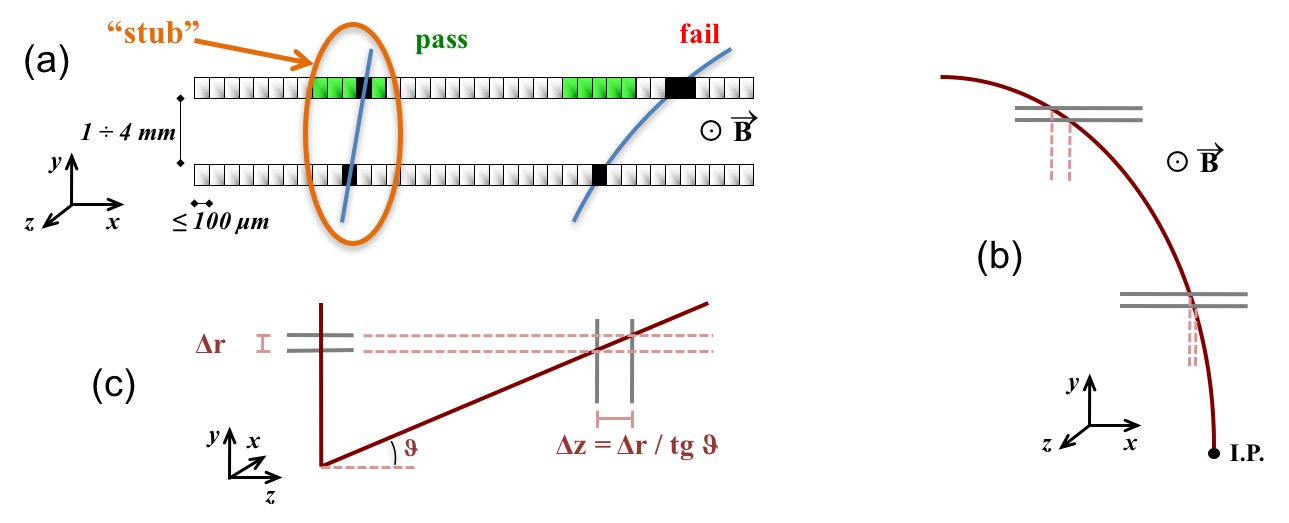
\includegraphics[width=5in]{figs/tk-upgrade/pTsketches.png}
% where an .eps filename suffix will be assumed under latex,
% and a .pdf suffix will be assumed for pdflatex; or what has been declared
% via \DeclareGraphicsExtensions.
\caption{Cluster matching in the $\pT$-modules proposed for the Outer Tracker~\cite{P2TrackerTDR} as described in the text; (a) demonstrates how correlating pairs of closely-spaced clusters between the two sensor layers allows for the discrimination of a track candidate's transverse momentum; (b) shows that if the sensor spacing remains unchanged, that the separation between the two clusters increases the further a module is away from the beam line; and (c) illustrates that the sensor spacing of modules in the endcap disks, which are perpendicular to the beam line, is required to be larger because of projective effects.
}
\label{fig:stubs}
\end{figure}

By correlating pairs of clusters on-detector that are consistent with a track with a transverse momentum of about 2\GeV or greater, an effective data rate reduction of approximately a factor of 10 is achieved before the resultant \emph{stubs} are transferred to the L-1 trigger~\cite{mpessimperf,2dptmoduleconcept}.

Two \pT modules are being developed for the Outer Tracker upgrade: 2S \emph{strip-strip} modules and PS \emph{pixel-strip} modules.
The 2S~modules, are designed to be used at radii $r>60$\cm from the beam line, where the hit occupancies are lower and each sensor has an active area of 0.05\cm~$\times$~9.14\cm.
Both 2S~module strip layers have a pitch of 90\mum in the transverse plane ($r$-$\varphi$) and a strip length of 5.03\cm along the direction of the beam axis, $z$.
Each PS~module sensor layer has an active area of 4.69\cm~$\times$~9.60\cm and will be used at radii in the range  $20<r<60$\cm where the occupancies are highest.
The upper PS~module layers consist of a silicon strip sensor and a silicon pixel sensor, both with a pitch of 100\mum in $r$-$\varphi$, and a strip length in $z$ of 2.35\cm for the strips and 1.47\mm for the pixels.
The finer granularity provided by the pixel layer affords better resolution along the $z$ axis, which is crucial for vertex identification in the high \PU environment of the HL-LHC.
Further details on the two \pT modules can be found in~\cite{CMS_Upgrade_TP,P2TrackerTDR}.

The current proposed layout of the Phase-II Outer Tracker, referred to as the \emph{tilted barrel} geometry, is depicted in the upper diagram in figure~\ref{fig:trackerlayout}, and a previous proposal, referred to as the \emph{flat barrel} geometry, is shown in the lower diagram~\cite{CMS_Upgrade_TP}.
Both plots illustrate the PS and 2S module positions in the six barrel layers and the five endcap disks on either side of the barrel, with only modules located at $|\eta| < 2.4$ being configured to send stub data off-detector.
The geometries are so named as they were inspired by whether or not the modules in the three innermost barrel layers are tilted so that their normals point towards the interaction region.
The advantages of the tilted geometry over the original flat barrel are that it not only improves stub-finding efficiency for tracks with large incident angles but also reduces the overall cost of the system~\cite{P2TrackerTDR}.
Due to the maturity of the preparations for the review between the three competing proposed track finder systems, discussed later in Section~\ref{subsec:TrackFinderReview}, at the time the tilted barrel geometry was adopted for the Phase-II Outer Tracker TDR it was decided to use the flat barrel geometry for results produced for the review.

\begin{figure}[tbp]
\centering
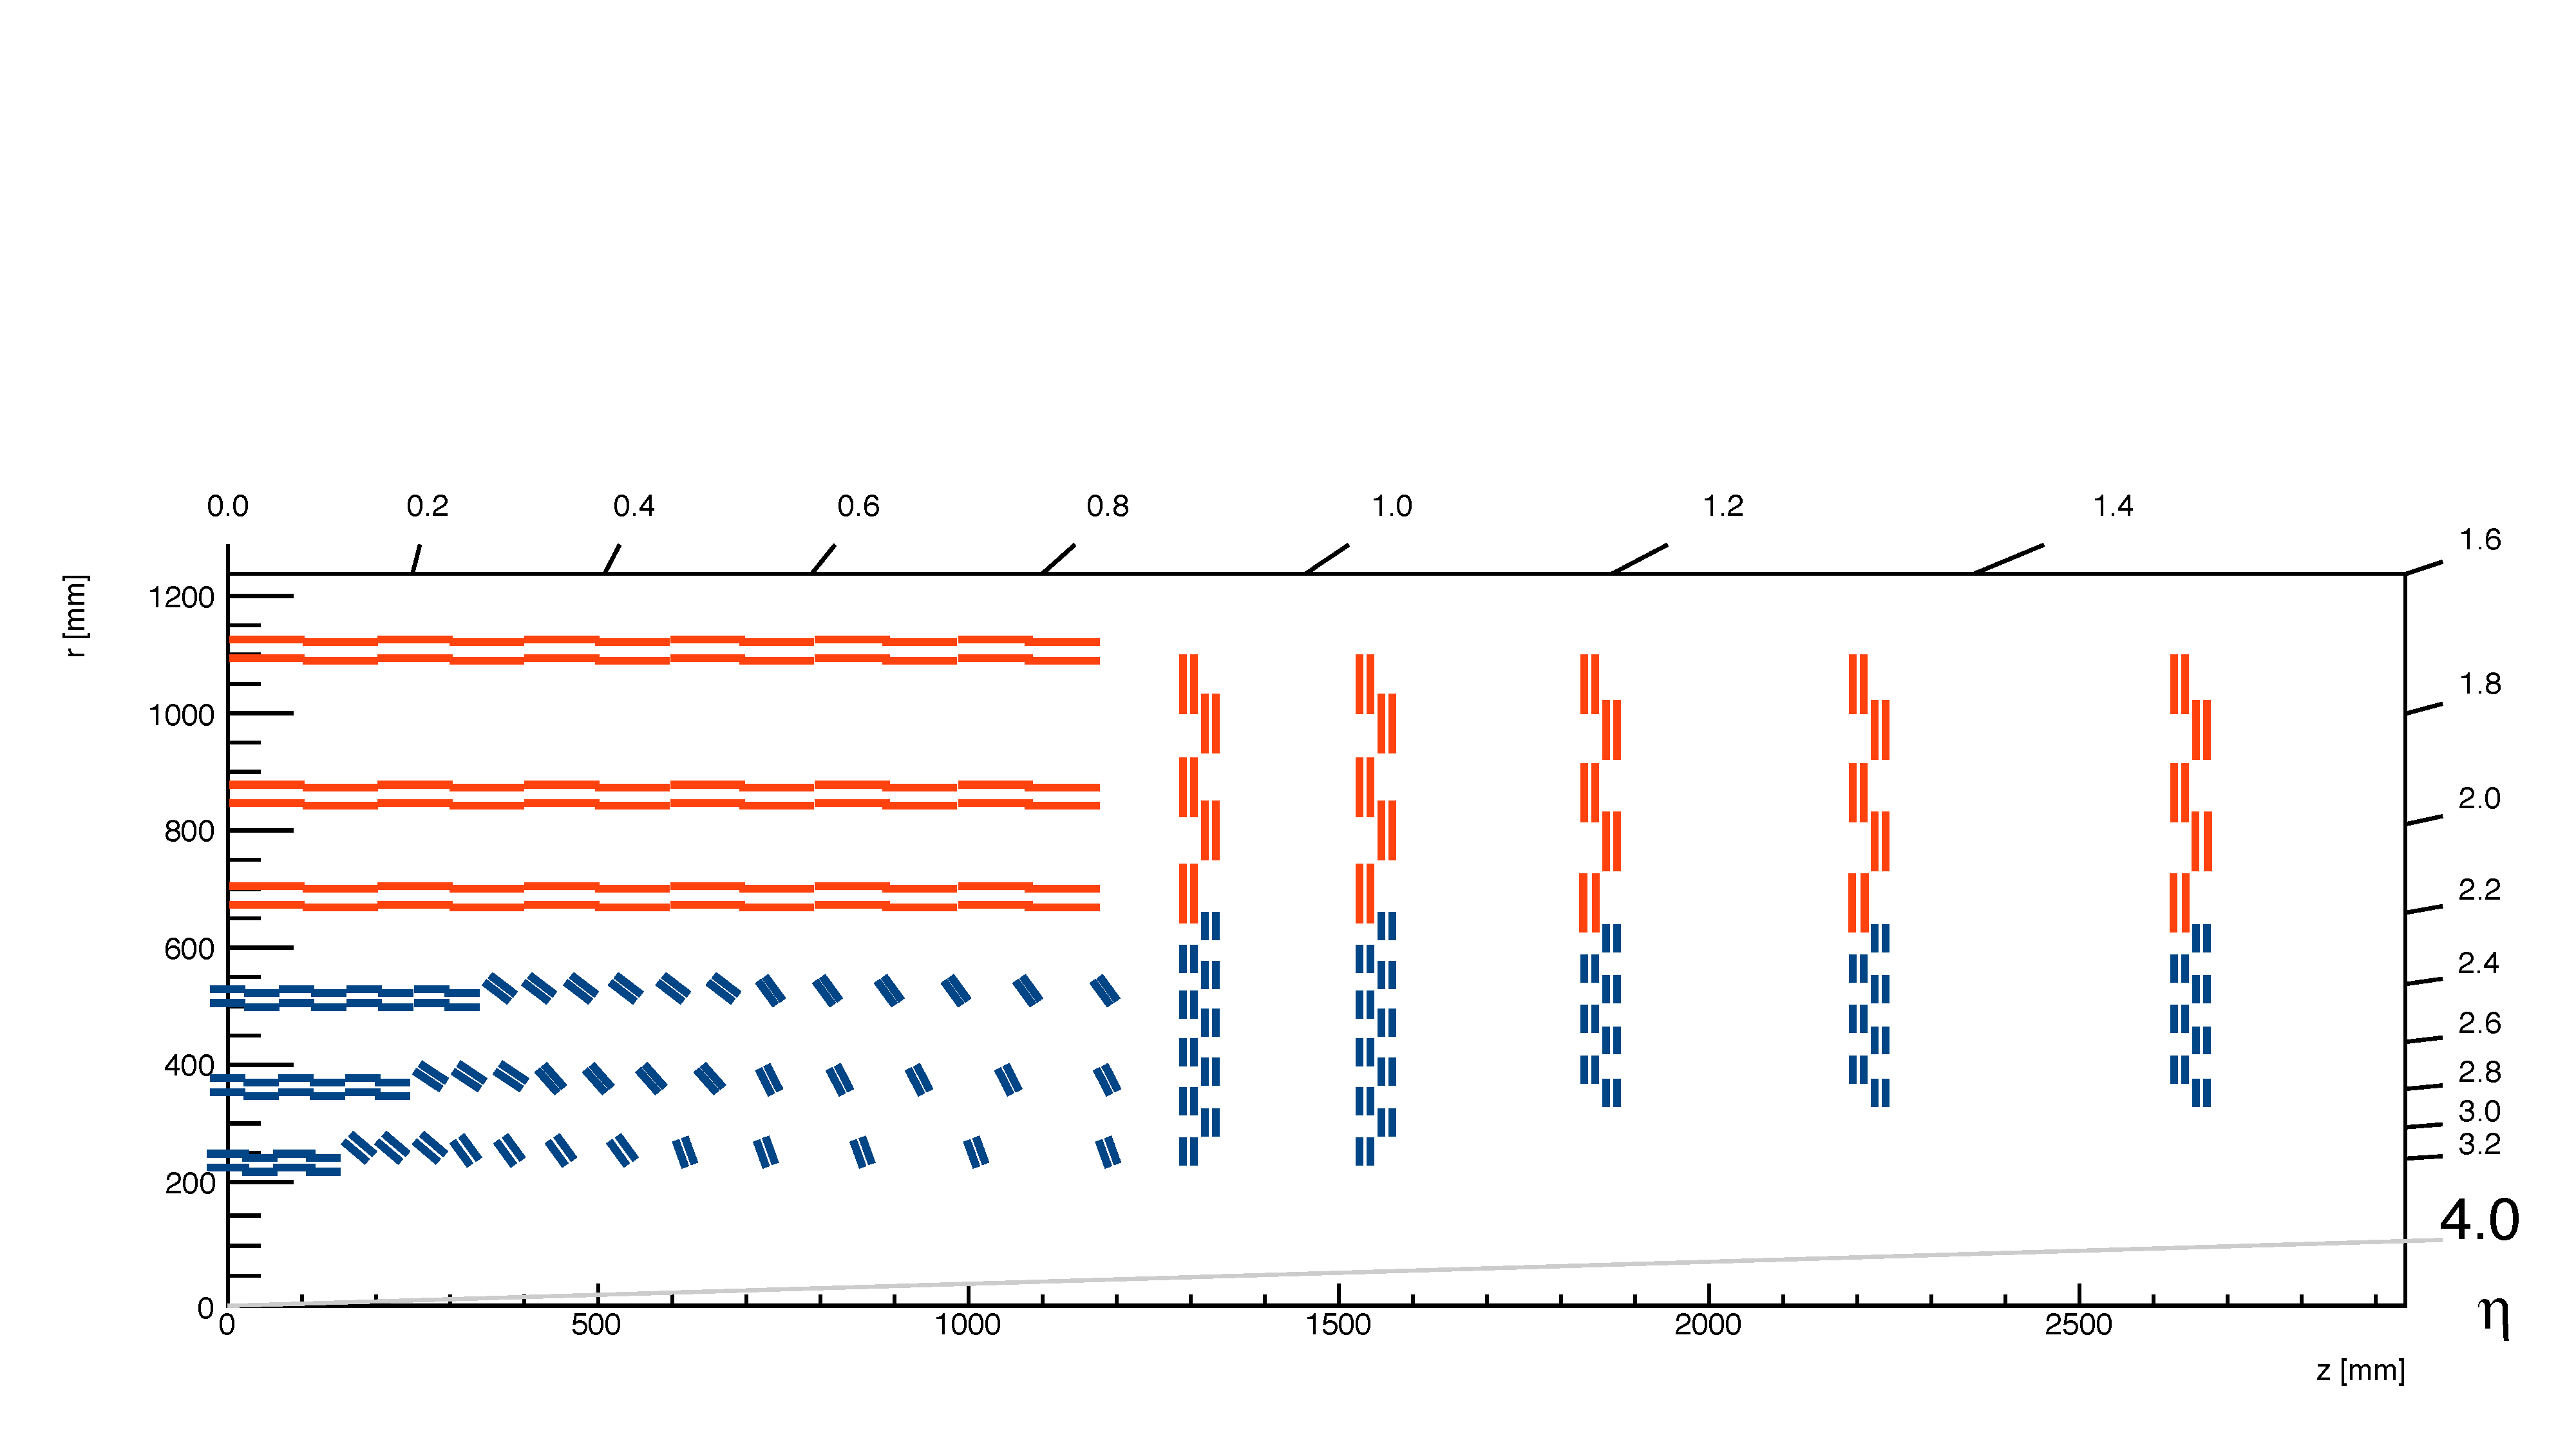
\includegraphics[width=0.8\textwidth,trim={1.1truecm 0truecm 1truecm 12truecm},clip]{figs/tk-upgrade/tiltedbarrelmap.pdf}
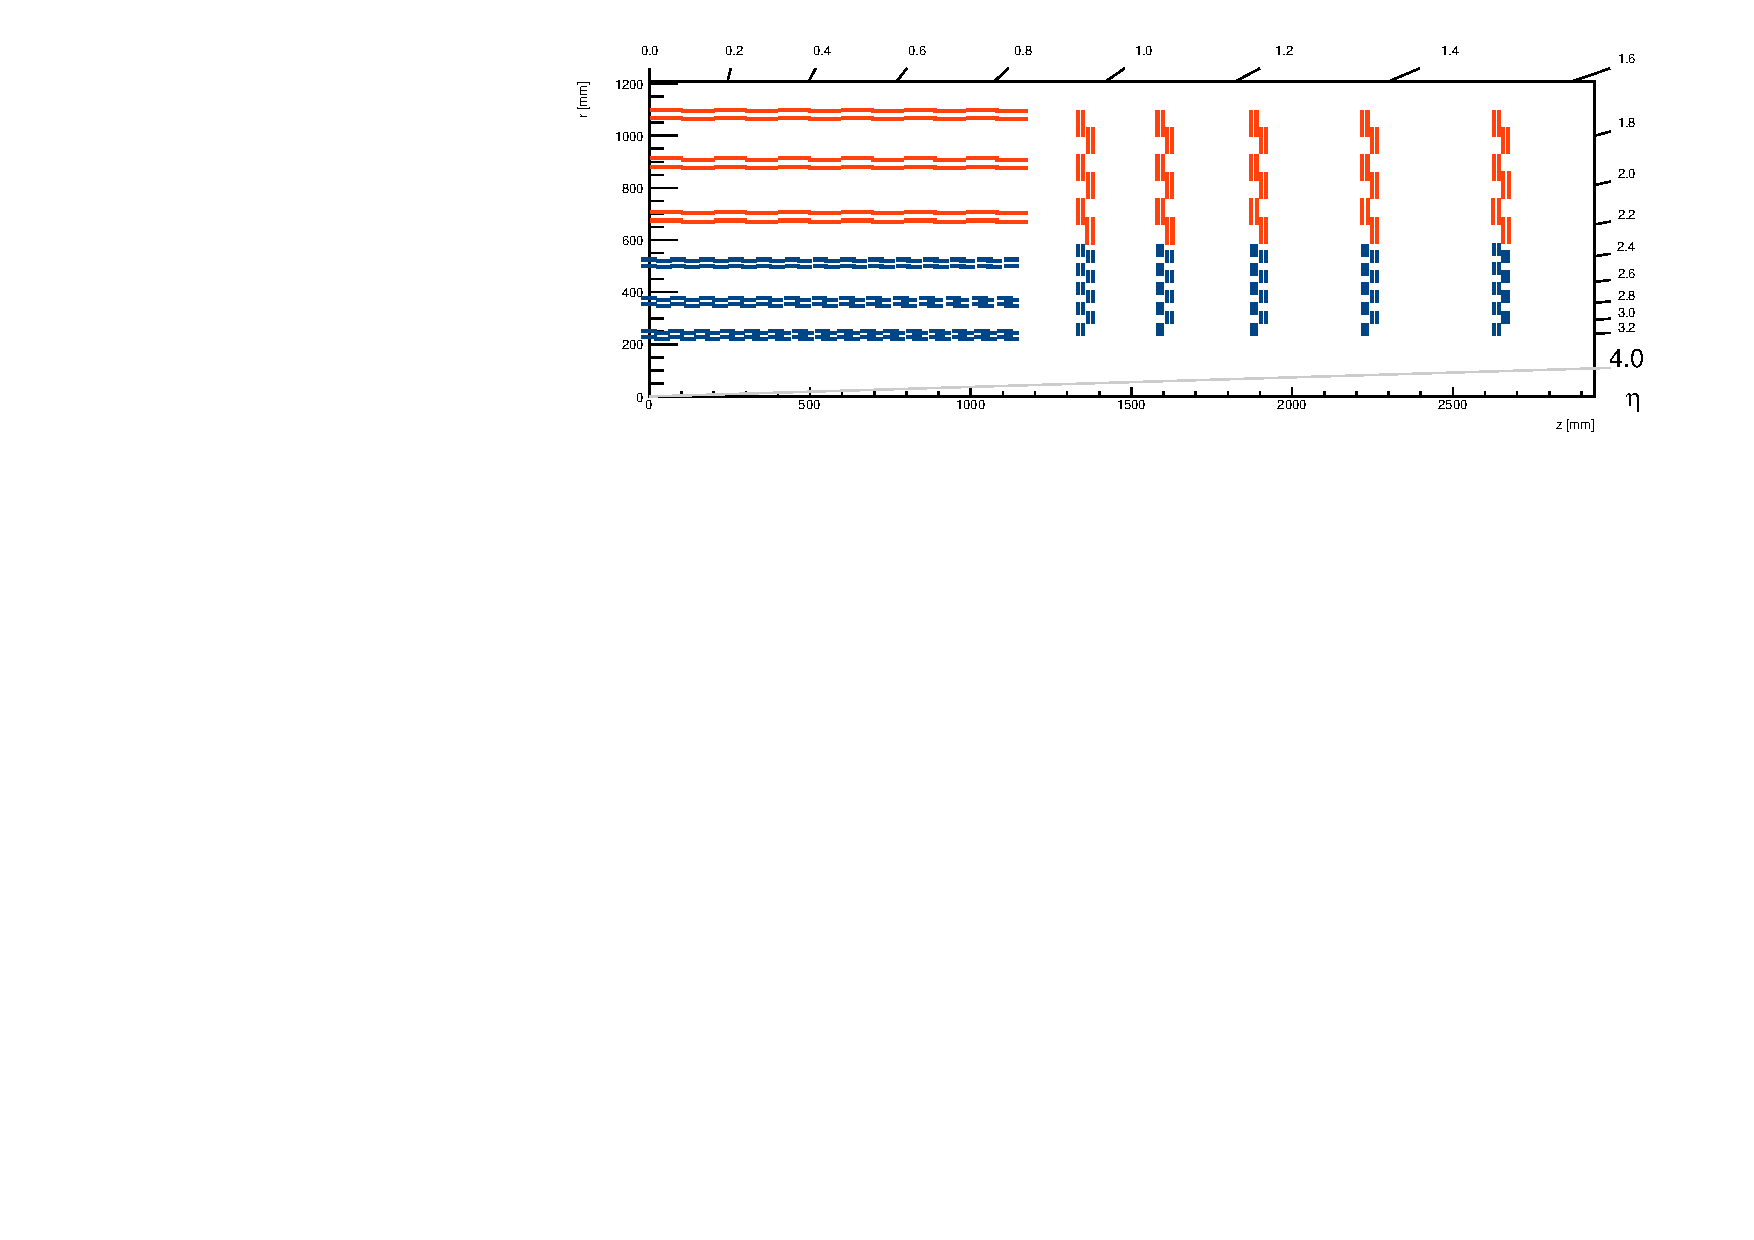
\includegraphics[width=0.8\textwidth,trim={0.7truecm 0truecm 1truecm 0truecm},clip]{figs/tk-upgrade/mersilayout.pdf}
\caption{One quadrant of the Phase-II Outer Tracker layout, showing the placement of the the PS (blue) and 2S (red) modules. The upper diagram shows the currently proposed \emph{tilted barrel} geometry~\cite{tiltedGeometry, P2TrackerTDR}, and the lower diagram shows an older proposal for the layout, known as the \emph{flat barrel} geometry \cite{CMS_Upgrade_TP}.}
\label{fig:trackerlayout}
\end{figure}

Figure ~\ref{fig:dataFlow} illustrates the data flow through the constituent parts of the track finding system and the latency available for each component.
The total L-1 latency is limited to 12.5\mus, of which 

The tracker front-end (FE) electronics require about $1\mus$ for the generation, packaging and transmission
of stubs to the Data, Trigger and Control (DTC) system.
Approximately $4\mus$

Out of the total L-1 latency of 12.5\mus, about $1\mus$ is required for generation, packaging and transmission of stubs from the tracker front-end (FE) electronics to the  system and approximately $4\mus$ is available for the reconstruction of tracks from data arriving at the DTC, as shown in figure~\ref{fig:dataFlow}.

\begin{figure}[tbp]
\centering
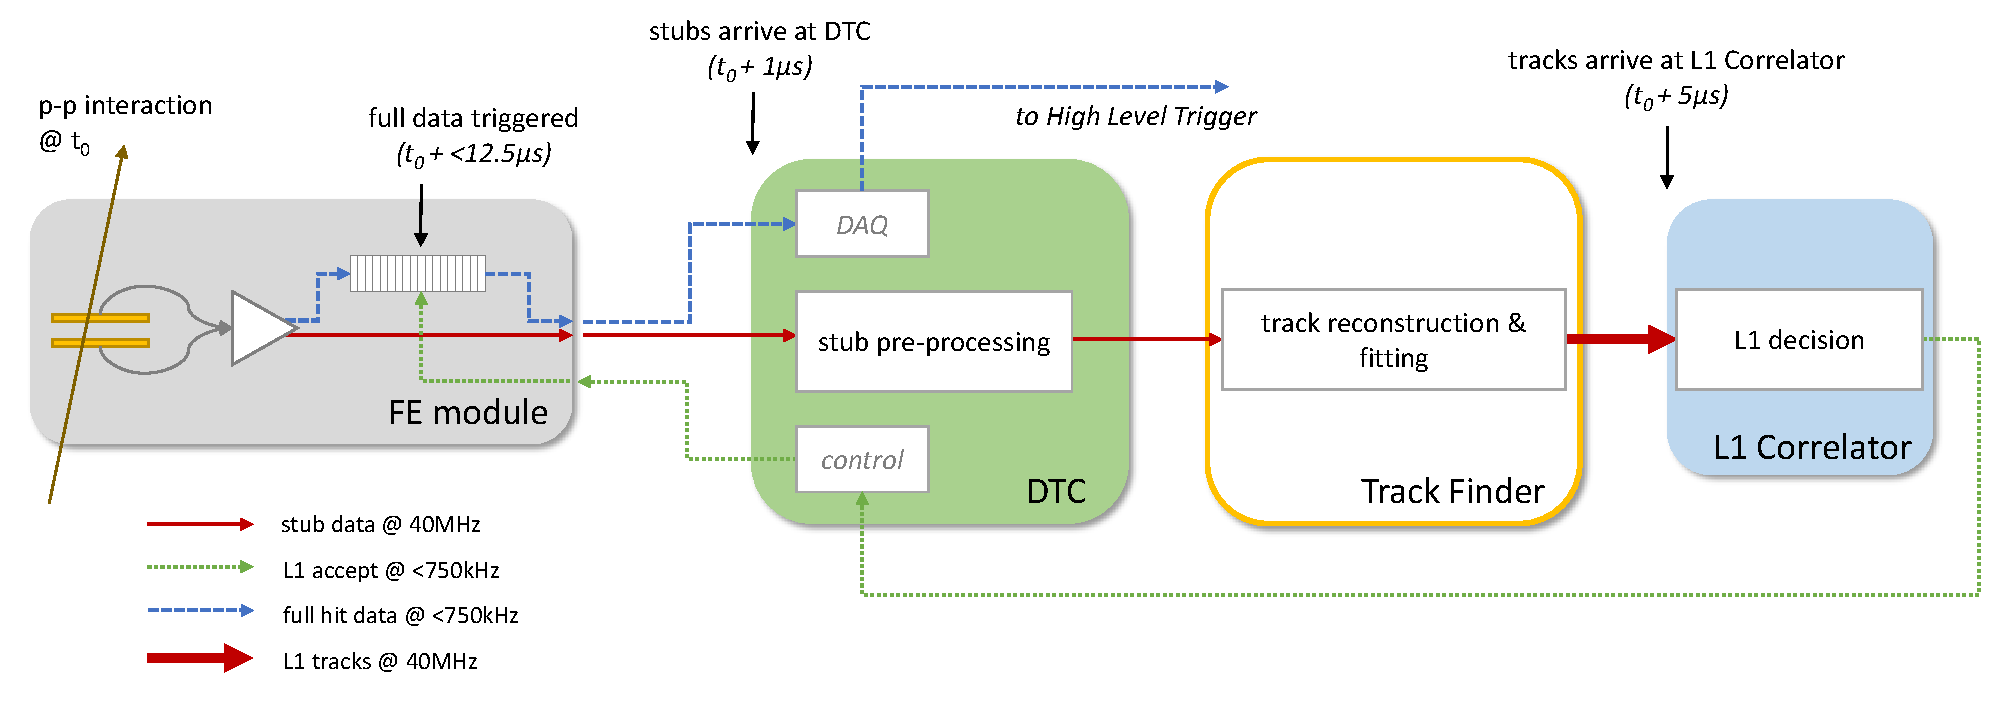
\includegraphics[width=\textwidth]{figs/tk-upgrade/dataflow.pdf}
% where an .eps filename suffix will be assumed under latex,
% and a .pdf suffix will be assumed for pdflatex; or what has been declared
% via \DeclareGraphicsExtensions.
\caption{Illustration of data flow and latency requirements starting from the \pt-modules and front-end (FE) electronicds and running through to the off-detector electronics dedicated to forming the L-1 trigger decision.}
\label{fig:dataFlow}
\end{figure}

The rest of the available latency is allocated for the correlation of tracks with trigger primitives from the calorimeters and muon systems ($3.5\mus$), the propagation of the L-1 decision to the front-end buffers ($1\mus$) and a safety margin ($3\mus$)~\cite{CMS_Upgrade_TP}.

The architecture of any Track Finder system proposed, which will take the pre-processed stubs as input and output fully reconstructed tracks for the L-1, will be constrained by the system's latency budget and how the detector is cabled to the DTC system.
The $4\mus$ latency constraint will limit the amount of processing that can be done for the finding and fitting of tracks and the choice of cabling scheme for the detector will determine how data is distributed and processed throughout the Track Finder system.

\subsection{Level-1 Track Finding Proposals}\label{subsec:TrackFinderReview}

Three different L-1 track finders have been explored by the CMS Collaboration.
One uses Associative Memory (\emph{AM}) ASICs for track finding and FPGAs for track fitting, and the other two all-FPGA approaches, one using a fully Time-Multiplexed Track (\emph{TMT})finder which uses the Hough Transform to identify track candidates and one using a ``road search'' (\emph{tracklet}) algorithm to reconstruct tracks.

Hardware demonstrators for each of the three proposed L-1 track finder projects were constructed to prove the feasibility of each approach, which were reviewed in 2016.
As all of the work discussed in this chapter was on the FPGA-based \HT approach.
More detailed descriptions and results of both the AM and tracklet projects' approaches are not discussed here, but are given in earlier references~\cite{P2TrackerTDR,AM} and~\cite{P2TrackerTDR,tracklet} respectively.

As mentioned in Section~\ref{sec:tk-upgrade}, at the time of the review the flat barrel geometry described earlier was used for all the studies undertaken, as depicted in the lower diagram in figure~\ref{fig:trackerlayout}.
As such, unless stated otherwise, the results discussed below use the flat barrel geometry instead of the current tilted geometry.

\section{A Time-Multiplexed Track Finder }\label{sec:TMTT}
The Time-Multiplexed Track finder 

\subsection{The Track Finding Architecture}\label{subsec:TFA}
The proposed FPGA-based Hough Transform Track Finder is a scalable, flexible and redundant design based on a fully time-multiplexed architecture for implementation on commercially available FPGAs, as previously demonstrated by the Phase-I Calorimeter Trigger Upgrade~\cite{Tapper:2013yva} discussed in Section~\ref{paragraph:L-1}.
As discussed in Section~\ref{paragraph:L-1}, a time-multiplexed design has a number of advantages, including that only a single Track Finding Processor (TFP) is required to demonstrate the full system as each processor is identical in every respect.

Unlike the Phase-I Calorimeter Trigger, it is not feasible to process the entire output of the Phase-II Outer Tracker in a single processor for a given time slice because of the limits imposed by the input and total bandwidth a single FPGA-based processor can handle.
Therefore, as it was assumed at the time of the 2016 review that the DTC system would be arranged such that it forms octants~\footnote{These detector octants are not uniform as the geometry of the tracker does not have an exact eight-fold symmetry} (\ie 45 degree $\varphi$-sectors, referred to as \emph {detector octants}) in the tracker, the baseline system proposed was divided into \emph{processor octants} that were offset from the detector octants by $\approx 22.5$ degrees in $\phi$, in order to handle data duplication across hardware boundaries.
This baseline system architecture, illustrated in figure~\ref{fig:tmttarch}, uses two neighbouring DTCs to time-multiplex and duplicate stub data across processing octant boundaries before each DTC transmits 50\% of its data to one TFP and 50\% to the neighbouring TFP.
Based on current electronics and the high speed links available, the data requires 18 TFPs per processing octant (one for each time slice, resulting in a full system requiring 144 TFPs).

\begin{figure}[t]
\centering
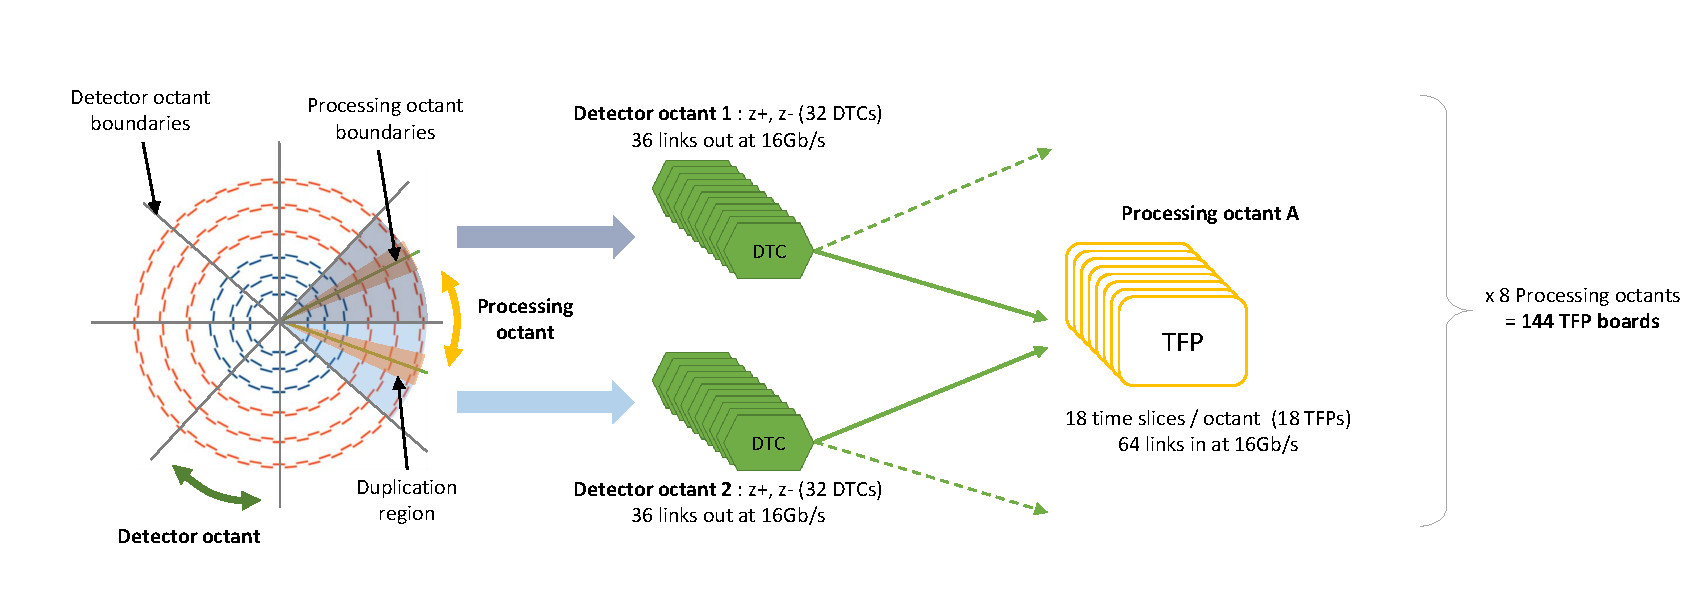
\includegraphics[width=1.00\textwidth]{figs/tk-upgrade/tmttarch.pdf}
\caption{An illusratation of the baseline system architecture described in the text, demonstrating how two neighbouring DTCs time-multiplex and duplicate stub data across processing octants and how it transmits the processed data to two neighbouring TFPs~\cite{TMTT_JINST}}
\label{fig:tmttarch}
\end{figure}

A hardware demonstrator of the baseline system consisting of five Imperial Master Processor Virtex-7 (MP7) cards~\cite{mp7ref}, capable of processing one phi-octant of the tracker with a time-multiplexing factor of 36, was used to validate the feasibility of the proposed full system using hardware available at the time of the 2016 review.
All of the results achieved, and a complete description of the system, are given in~\cite{TMTT_JINST}.

\subsection{The Track Finding Processor}\label{subsec:TFP}
The Track Finding Processor shown in figure~\ref{fig:TFP} consists of four self-contained components:
\begin{itemize}
\item {\bf Geometric Processor (GP)} Responsible for pre-processing the stubs from the DTC.
\item {\bf Hough Transform (HT)} A highly parallelised initial coarse track finding.
\item {\bf Kalman Filter (KF)} Removes incorrectly associated stubs from a track, precisely fits helix parameters and removes fake tracks.
\item {\bf Duplicate Removal (DR)} A final pass filter that uses the precise fit information to remove duplicate tracks generated by the \HT.
\end{itemize}

Each of these components is described in more detail below.

\begin{figure}[!h]
\centering
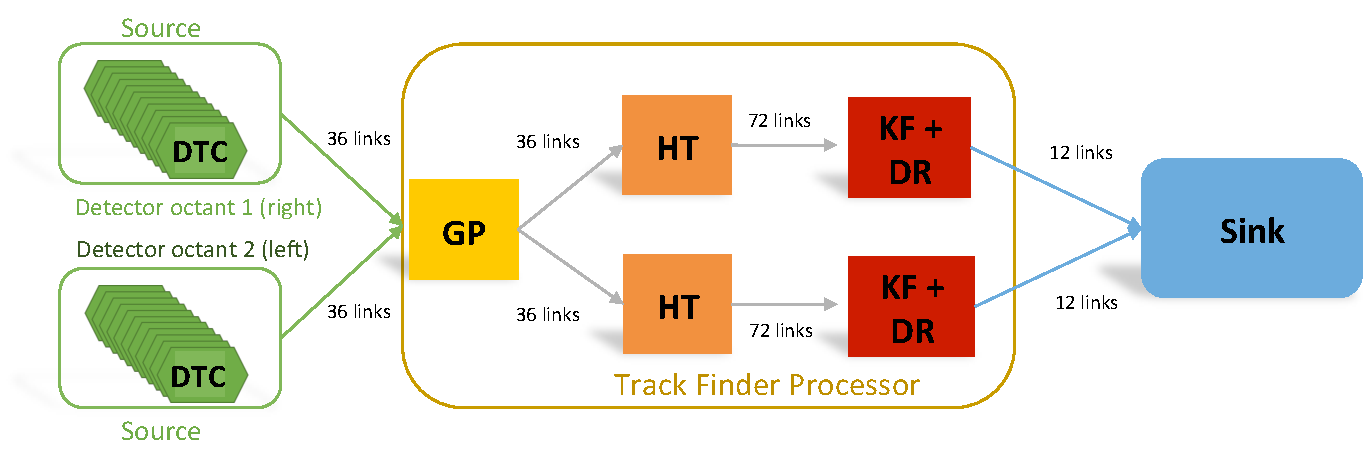
\includegraphics[width=0.78\textwidth]{figs/tk-upgrade/demoslice1.pdf}
% where an .eps filename suffix will be assumed under latex,
% and a .pdf suffix will be assumed for pdflatex; or what has been declared
% via \DeclareGraphicsExtensions.
\caption{The four self-contained logical components of the Track Finding Processor, where each box (block) in the diagram represents a single FPGA. The two FPGAs for the two detector octant sources and the sink FPGA and the optical links between all components are also shown.}
\label{fig:TFP}
\end{figure}

\subsubsection{Geometric Processor}\label{subsubsec:GP}
Each GP performs two tasks: the conversion of the 48-bit DTC stubs into a 64-bit format extended format that is used to reduce the HT processing load and assignment of the stubs in each sector into a subsector. 
Each sector is composed of 2 sub-sectors in $\phi$ and 18 in $\eta$.

This division of the processing octants simplifies the task of the downstream logic, allowing the track finding to be carried out independently and in parallel within each sub-sector. 
The chosen $\eta$ binning is sufficiently fine to ensure that any track found by the \rphi HT is consistent with a straight line in the \rz plane, despite the fact the \HT itself only searches for tracks in the \rphi plane, thus rejecting incompatible track candidates.

Stubs that are compatible with more than one sub-sector, usually due to track curvature in $\phi$, are duplicated. 

Stubs are assigned to sub-sectors occurs in a three stage process:
\begin{itemize}
\item A rough $\eta$ sorting into six bins;
\item A subsequent fine $\eta$ sorting into three bins and;
\item A $\phi$ sorting into two bins. 
\end{itemize}

Each of the TFP's logic blocks shown in figure~\ref{fig:TFP} has been designed to be highly reconfigurable and can easily be adapted to any alternative sub-sector definition.

\subsubsection{Hough Transform}
The Hough Transform algorithm is a widely used means of detecting geometric features in digital image processing~\cite{HT}.

%%% GENERAL INTRO

The \HT is used by the TFP to find charged particles with $\pT > 3\GeV$ in the \rphi plane. 

Initially we consider for a tracking volume, permeated by a homogeneous 3.8T magnetic field ($B$), a track with a radius of curvature ($R$) can be described as a function of its \pT and charge $q$:

\begin{equation}
R = \frac{\pt}{0.003\,qB} \;
\label{eq:R}
\end{equation}

Assuming, to first order, that $R$ is constant, by neglecting energy losses such as through multiple scattering, and that only primary tracks from or near the primary interaction point are considered (other such tracks are not typically relevant to the L-1 trigger), a stub with coordinates ($r$,$\varphi$) is related to $R$ by:

\begin{equation}
\frac r{2\,R} = \sin\left(\varphi-\phi\right) \;
\label{eq:stub_R}
\end{equation}

where $\phi$ is the angle of the track in the transverse plane at the origin \cite{markthesis}. 
For large \pT ($> 3\GeV$) and thus large $R$, the small angle approximation can be used. Combining Equations~(\ref{eq:R}) and (~\ref{eq:stub_R}), one produces the key formula showing the transformation from stub positions to straight lines in the track parameter plane (Hough-space):

\begin{equation}
\phi = \varphi - \frac{0.0015\,qB}{\pt}\cdot r \;
\label{eq:localHT}
\end{equation}

The point of intersection of these lines in Hough-space would therefore correspond to a circle in the \rphi plane which is consistent with the primary interaction point and all stubs involved.
As the line gradients in Hough-space is given by the radius of the stubs, they will always be positive, the stub radius is transformed to $r_{58} = r - 58cm$ in order to utilise a larger phase space, which leads to fewer \textit{fake} (in that the found track does not match to a simulated particle) and duplicated tracks.

Given that $R$ for the lowest \pT track (3\GeV) to be considered is greater than the outer radius of the tracking detector ($r$ = 1.2m), all relevant particles are expected to traverse through at least six barrel layers or endcap disks. 
The threshold for the identification of a track candidate however, is set at a minimum of five detector layers or disks in order to allow for detector or readout inefficiencies. 
This threshold can be further reduced to four layers to account for the reduced geometric coverage between $0.89 < \eta < 1.16$ or for dead detector layers or disks.

A more detailed description of the firmware implementation of the \HT for the demonstrator system is discussed in~\cite{TMTT_JINST,IEEE}.

\subsubsection{Kalman Filter}\label{subsubsec:KF}
\editComment{More detail - including on the covariance matrix ...}
The coarse \rphi helix parameters that are output by the \HT are used as the initial variables for track finding, with the segment assignment also providing a good seed value.
Given that in simulation over half the track candidates from by the HT are considered to be \textit{fake} or contain at least one stub associated with another particle, a Kalman Filter is used to both remove these incorrect stubs and reject fake tracks. 

In addition to the advantages of the Kalman filter for track reconstruction discussed by Fr{\"u}hwirth in \cite{Fruhwirth:1987fm}, the algorithm has several aspects making it suitable for FPGA implementation compared to global track fitting methods, namely the matrices:

\begin{itemize}
\item {are small.}
\item {are sized independently of the number of measurements.}
\item {only involve the inversion of a small matrix.}
\end{itemize}

The initial estimates, or \textit{state}, of the track parameters and their uncertainties, $\chi^2$ value and other status information are updated by the KF iteratively applying stubs to update the state following the Kalman formalism, decreasing the uncertainty in the state. 
Each update of the state can be filtered on number of configurable criteria, including \pT, $\chi^2$, and the minimum number of stubs from PS modules, and can take into account and skip missing missing layers due to missing or incorrect stubs.
In the event multiple stubs are found on the same layer, each can be propagated with up to the four best states being kept and presented to a final state selector, with preference given to states with the fewest missing layers and the smallest $\chi^2$.
The final fit is always performed after a fixed period of time, so consequently there is no truncation in the traditional sense as all candidates will be read out, although events such as dense jets with many candidates and stubs per candidate will only be partially filtered.

A greater in-depth discussion of the mathematics and implementation of online track reconstruction using Kalman Filters on FPGAs in~\cite{SSummers}.

\subsubsection{Duplicate Removal}
Following the \KF, over half of the track candidates are unwanted duplicate tracks created by the HT.
Instead of comparing pairs of tracks to see if they are the same, a more elegant and subtle DR algorithm is used which takes into account how the \HT produces these duplicate tracks.
This approach is illustrated in figure~\ref{fig:DR}, where five stubs, which correspond to the blue lines in Hough Space, produce candidates in the green and two yellow cells.
The coarse track finding performed by the \HT 

however, as all three candidates contain the same stubs, they will be fitted with identical helix parameters in the same cell (the yellow cell) regardless of the original HT cell.


The DR algorithm accepts only tracks whose fitted parameters are consistent with the \HT cell in which they were initially found. 
There is however, a small subtlety, given that the algorithm eliminates unique tracks whose fitted parameters were not consistent, which results in the loss of a few percent of efficiency. 
By performing a second pass through the rejected tracks, tracks which have fitted parameters that do not correspond to the HT cell of a track from the first pass are probably not duplicates, and so they are recovered.

\begin{figure}[!h]
\centering
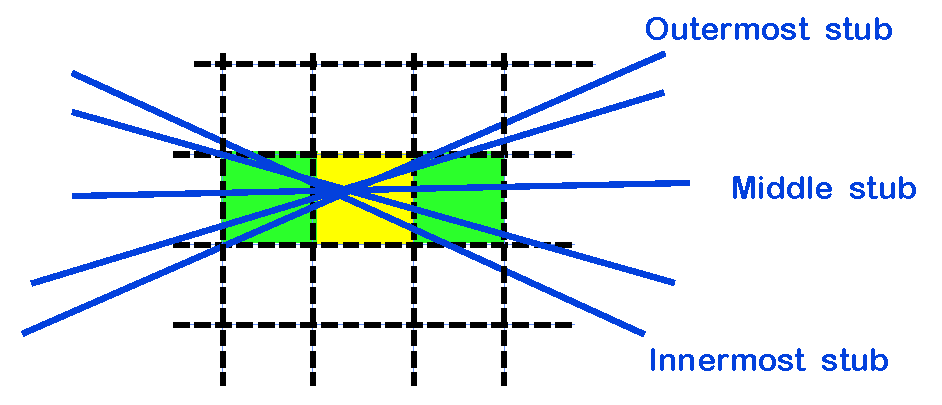
\includegraphics[width=0.80\textwidth]{figs/tk-upgrade/A50_algo.pdf}
% where an .eps filename suffix will be assumed under latex,
% and a .pdf suffix will be assumed for pdflatex; or what has been declared
% via \DeclareGraphicsExtensions.
\caption{Illustration of how duplicates are formed by the \rphi \HT.}
\label{fig:DR}
\end{figure}

A more detailed description of the firmware implementation of the \DR for the demonstrator system is discussed in~\cite{TMTT_JINST}.

\section{Simulation Studies}\label{sec:TmttSimStudies}
This section presents a number of simulation studies which were undertaken as part of the development of the \emph{TMT} finder demonstrator system both before and following the 2016 review.
All of the results discussed use a common set of definitions, as defined in Section~\ref{subsec:helixParameter}, and the track fitters discussed use digitised output from the \HT.

\subsection{Definitions}\label{subsec:helixParameter}
A number of parameters and metrics are used throughout this chapter to describe tracks and how well the track fitters have reconstructed them.
They are defined as below.

\subsubsection{Helix Parameters}
The helical trajectory of a charged particle at the impact point is described by five helix parameters.
In the CMS these parameters are defined as:

\begin{itemize}
\item $\mathbf{p_{T}}$ - the transverse momentum of the track;
\item $\mathbf{\phi_{0}}$ - the track angle in the transverse plane;
\item $\mathbf{z_{0}}$ - the \emph{longitudinal} impact parameter, \ie the distance in z from the point of closest approach to the interaction point;
\item $\mathbf{\cot(\theta)}$ - the cotangent of the \emph{dip} (polar) angle, related to $\eta$ by $\cot(\theta) = \sinh (\eta)^{-1}$;
\item $\mathbf{d_{0}}$ - the \emph{transverse} impact parameter, \ie the distance of the track vertex from the interaction point in the $x-y$ plane. 
\end{itemize}

As the \HT and track fitting algorithms discussed all assume that all tracks originate at the interaction point, $d_{0}$ is not given in the results below as it is fixed to zero.

\subsubsection{Reconstructed Tracks}
The common definitions of track reconstruction efficiency~\cite{TMTT_JINST} used for the three proposed L-1 Track Finder systems are used for the results presented in this chapter:

\begin{itemize}
\item The reconstruction efficiency ($\epsilon$) is measured relative to all generated charged particles from the primary interaction that produce stubs in at least four layers of the tracker which satisfies the following conditions: $\pT > 3\GeV$, $|\eta| < 2.4$, $|z_{0}| < 30\cm$ and $d_{xy} < 1\cm$, where $d_{xy}$ is the distance in the $x-y$ plane from the point of closest approach to the interaction point.
\item A track is a defined as being correctly reconstructed or \emph{matched} if the reconstructed track has stubs associated to the particle in at least four tracker layers. Tracks which fail this matching criteria are known either as \emph{unmatched} or \emph{fake} tracks.
\item If the reconstruction of a charged particle produces more than one track, these additional tracks are considered to be \emph{duplicates}.
\item If all a reconstructed track's stubs originated from the same particle, the track is defined as being \emph{perfectly} reconstructed ($\epsilon_{P}$). 
\end{itemize}

This stricter definition of \emph{perfect} track reconstruction efficiency is typically used in quoting results from the entire chain (\ie all four components of the TFP discussed in Section~\ref{subsec:TFP}).
Otherwise, the nominal definition of track reconstruction efficiency is used as the presence of stubs incorrectly associated with a track is to be expected if only part of the TFP chain has been run.
Where appropriate, the results for both definitions are given.


\subsection{Linearised $\chi^{2}$ Track Fitter}\label{subsec:chi2}

Three different track fitting algorithms were explored for the track fitter to be used for the 2016 hardware demonstrator review: a Kalman Filter, a Linear Regression (LR) algorithm and a linearised $\chi^{2}$ track fit.

The development of a Kalman Filter track fitter was motivated by its ability to filter 
 
As it provided the best perfect track reconstruction efficiency and fake track rejection rate out of the three fitting algorithms explored, it was selected as the baseline fitter for the 2016 review.

The Linear Regression (LR) algorithm~\cite{TMTT_FLP} was developed as an alternative to the KF.
A LR fit is well suited to 
As sufficiently high \pT tracks should form a straight line in the \emph{\rphi} and \emph{r-z} planes, the fitting of these


this allows  LR algorithm	to perform independent fits in each plane.
While 

The studies of the linearised $\chi^{2}$ track fit were initially motivated by the \emph{TMT} project needing a track fitting algorithm which could be quickly implemented given the time and resource pressures in developing a hardware demonstrator for a complete track finder system for the 2016 review.

Following discussions with both the \emph{tracklet} and \emph{AM} projects, it was decided a linearised $\chi^{2}$ fit based on the algorithm proposed by the \emph{tracklet} project would be investigated.
The general form of the $\chi^{2}$ fit and the derivation of the track derivatives required by the algorithm were provided in a private communication~\cite{CMS_DN-14-043} and were used to produce a \emph{TMT} implementation of it.

A linearised $\chi^{2}$ fit calculates improved helix parameters for the track candidate by determining the  residuals between the stubs and the seeded track that minimise the $\chi^{2}$ of the fit.

The general form of the $\chi^{2}$ fit describing how these hit residuals are used to obtain a fit of a track's helix parameters is detailed in Section~\ref{subsubsec:chi2maths}.
A discussion of the development and outcomes of the software implementation of the fitting algorithm are given in Sections~\ref{subsubsec:chi2software} and~\ref{subsubsec:chi2outlook}.


The calculation of the track derivatives for the barrel layer hits and endcap disk hits used by the algorithm, included a correction factor for $\phi$ in the outer disks to account for the fact that these modules do not point directly towards the interaction point, which is described in Appendix~\ref{app:chi2}.

All the results presented here involve the use of a \emph{Seed Filter} (SF) stage that was run following the \HT stage for both the Linear Regression and Linearised $\chi^{2}$ fitting algorithms.
This process removes stubs in a \HT cell that are inconsistent with a straight line in the \emph{r-z} plane and filters out both fake tracks and stubs incorrectly assigned to tracks (also referred to as \emph{fake} stubs).

\subsubsection{General Form of a $\chi^{2}$ Fit}\label{subsubsec:chi2maths}
For the general form of a $\chi^{2}$ fit for a track, $f$, described by its helix parameters, $\overrightarrow{h}$, and the position of its hits (\ie stubs), $s_{i}$, we initially linearly expand the expected trajectory of the track, $f_{i}$, around the estimate of the helix parameters $\overline{h}$:

\begin{equation}
f_{i}(\overrightarrow{h} ) = f_{i}(\overrightarrow{h}) + \delta \overrightarrow{h}) \;
                           = f_{i}(\overline{h} + \delta \overrightarrow{h} \frac{\partial f_{i}}{\partial \overrightarrow{h}} + \mathcal{O}(\delta \overrightarrow{h}^{2}) \;
\label{eq:chi1}
\end{equation}

The $\chi^{2}$ of such a track is expressed as:

\begin{equation}
\begin{split}
\chi^{2} &= \sum_{ij} \big(f_{i}(\overrightarrow{h}) - s_{i} \big) V^{-1}_{ij}  \big(f_{j}(\overrightarrow{h}) - s_{j} \big)  \\
         &= \sum_{ij} \big( f_{i}(\overline{h})  - s_{i} + \delta \overrightarrow{h} \frac{\partial f_{i}}{\partial \overrightarrow{h}} \big) V^{-1}_{ij}  \big( f_{j}(\overline{h})  - s_{j} + \delta \overrightarrow{h} \frac{\partial f_{j}}{\partial \overrightarrow{h}} \big)  \\
         &= \sum_{ij} \big( \delta f_{i} + \delta \overrightarrow{h} \frac{\partial f_{i}}{\partial \overrightarrow{h}} \big) V^{-1}_{ij}  \big( \delta f_{j} + \delta \overrightarrow{h} \frac{\partial f_{j}}{\partial \overrightarrow{h}} \big)
\end{split}
\label{eq:chi2}
\end{equation}

where $\delta f_{i} \equiv f_{i}(\overline{h}) - s_{i}$ are the residuals between the expected position of the track (given by the seed helix parameters) and the position of the track given by the stub, and $V^{-1}_{ij} = diag(\sigma^{2}_{ii})$ is the variance matrix that describes the uncertainty associated with the measurement of the stubs.

By minimising the $\chi^{2}$, $\delta h$ can be determined:

\begin{equation}
0 = \frac{\partial \chi^{2}}{\partial \delta \overrightarrow{h_{k}}} = \sum_{ij} \frac{\partial f_{i}}{\partial \delta \overrightarrow{h_{k}}} V^{-1}_{ij} ( \delta f_{j} + \delta \overrightarrow{h} \frac{\partial f_{j}}{\partial \overrightarrow{h}} ) + \sum_{ij}	( \delta f_{i} + \delta \overrightarrow{h} \frac{\partial f_{i}}{\partial \overrightarrow{h}} ) V^{-1}_{ij} \frac{\partial f_{j}}{\partial \delta \overrightarrow{h_{k}}}  \;
\label{eq:chi3}
\end{equation}

By defining the matrices $D_{ij} = \frac{\partial f_{i}}{\partial h_{k}}$ and $M = D^{T} V^{-1} D$, Equation~(\ref{eq:chi3}) can be rewritten and solved for $\delta h$:

\begin{equation}
0 = D^{T} V^{-1} \delta f + M \delta h \Rightarrow \delta h = - M^{-1} D^{T} \delta f \;
\label{eq:chi4}
\end{equation}

Therefore Equation~(\ref{eq:chi4}) provides a simple linear form for how the track helix parameters should be updated for a set of residuals with respect to the seed track candidate.

Similarly the $\chi^{2}$ of the fit can also be expressed in a linear form:

\begin{equation}
\begin{split}
\chi^{2} &= (\delta f + D \delta h)^{T}(\delta f + D \delta h) \\
         &= (\delta f - DM^{-1}D^{T}\delta f)^{T} (\delta f - DM^{-1}D^{T}\delta f) \\
         &= \delta f^{T} (1- DM^{-1}D^{T}) (1- DM^{-1}D^{T}) \delta f \\
         &= \delta f^{T} (1- DM^{-1}D^{T}) \delta f \\
         &= \delta f^{T} \delta f - \delta f^{T} DM^{-1}D^{T} \delta f \\
         &= \chi^{2}_{seed} + \delta f^{T} D \delta \overrightarrow{h} 
\end{split}
\label{eq:chi5}
\end{equation}

As the linear forms of Equations~(\ref{eq:chi4}) and~(\ref{eq:chi5}) consist of repeated addition and multiplication operations of the matrices involved, they are naturally suitable for implementation on an FPGA.

This is because while FPGAs can easily perform such operations, potential complications arise when considering the calculation of the track derivatives that form the elements of $D$.
Determining these elements would not be trivial given the presence of a large number of division operations and trigonometric functions for the endcaps' derivatives.
Therefore, any implementation in firmware for an FPGA will require the use of lookup tables containing the precomputed values of the derivatives in order to quickly update a track's helix parameters without exceeding latency budgets.

\subsubsection{Results of a Software Implementation}\label{subsubsec:chi2software}
From equations~(\ref{eq:chi4}) and~(\ref{eq:chi5}) and the track derivatives derived in Appendix~\ref{app:chi2}, a software implementation of the linearised $\chi^{2}$ track fit algorithm was developed.
Initially this implementation used exact floating point mathematics in order to validate the algorithm, before a version using approximated expressions of the track derivatives was developed.
The motivation behind this was to reduce the number of variables that the matrix of derivatives would depend on in order to simplify (and reduce resources required for) any future tabulation of the matrix.

\begin{table}[htbp]
\topcaption {Track finding performance on simulated \ttbar events with a <PU> of 200, after the \HT and the full chain for  both the exact floating point and approximated calculations of the track derivatives used by the $\chi^{2}$ track fit.
The track finding efficiencies, $\epsilon$ and $\epsilon_{P}$, following each stage are given along with the mean number of tracks, $<N_{tracks}>$, and the fraction of those tracks that are either fake or duplicate tracks.
}

\label{tab:chi2-exactVsApprox}
 \centering
 \resizebox{\textwidth}{!}{
% This right-aligns numbers in column, but centers them under column title.
 \begin{tabular}{cccccc}
   \hline
   \bf{Stage} & \bf{$\bm{\epsilon}$ [\%]} & \bf{$\bm{\epsilon_{P}}$ [\%]} & $\bm{<N_{tracks}>}$ & \bf{Fakes [\%]} & \bf{Duplicates [\%]}  \\
        \hline
   HT &  97.0 & 43.1 & 351.2 & 43.9 & 37.0 \\  
   \hline
   $\chi^{2}$+DR & 95.0 & 85.8 & 86.4 & 15.7 & 9.5 \\
   (floating point) & & & & & \\
   \hline
   $\chi^{2}$+DR & 94.9 & 85.6 & 87.4 & 15.5 & 10.9 \\  
   (approximated) & & & & & \\   
%   \hline
%   KF+DR & 94.1 & 94.1 & 82.1 & 21.1 & 4.5 \\
   \hline
   
 \end{tabular}}
\end{table}

Table~\ref{tab:chi2-exactVsApprox} shows how the tracking performance between the floating point maths and ``approximated'' maths versions of the algorithm compare against each other and from the raw track finding output from the \HT.

It can be seen that whilst the \HT finds tracks with high efficiency, over half have at least one incorrectly associated stub and a significant number of the tracks found are fake or duplicated tracks.
Both floating point and approximated maths implementations give comparable results, indicating that the approximations made are acceptable.
The $\chi^{2}$ track fit increases the purity of the reconstructed tracks by a factor of two and eliminates the majority of the fake tracks, whilst the \DR algorithm removes the majority of the duplicates.


\begin{figure}[htb]
\centering
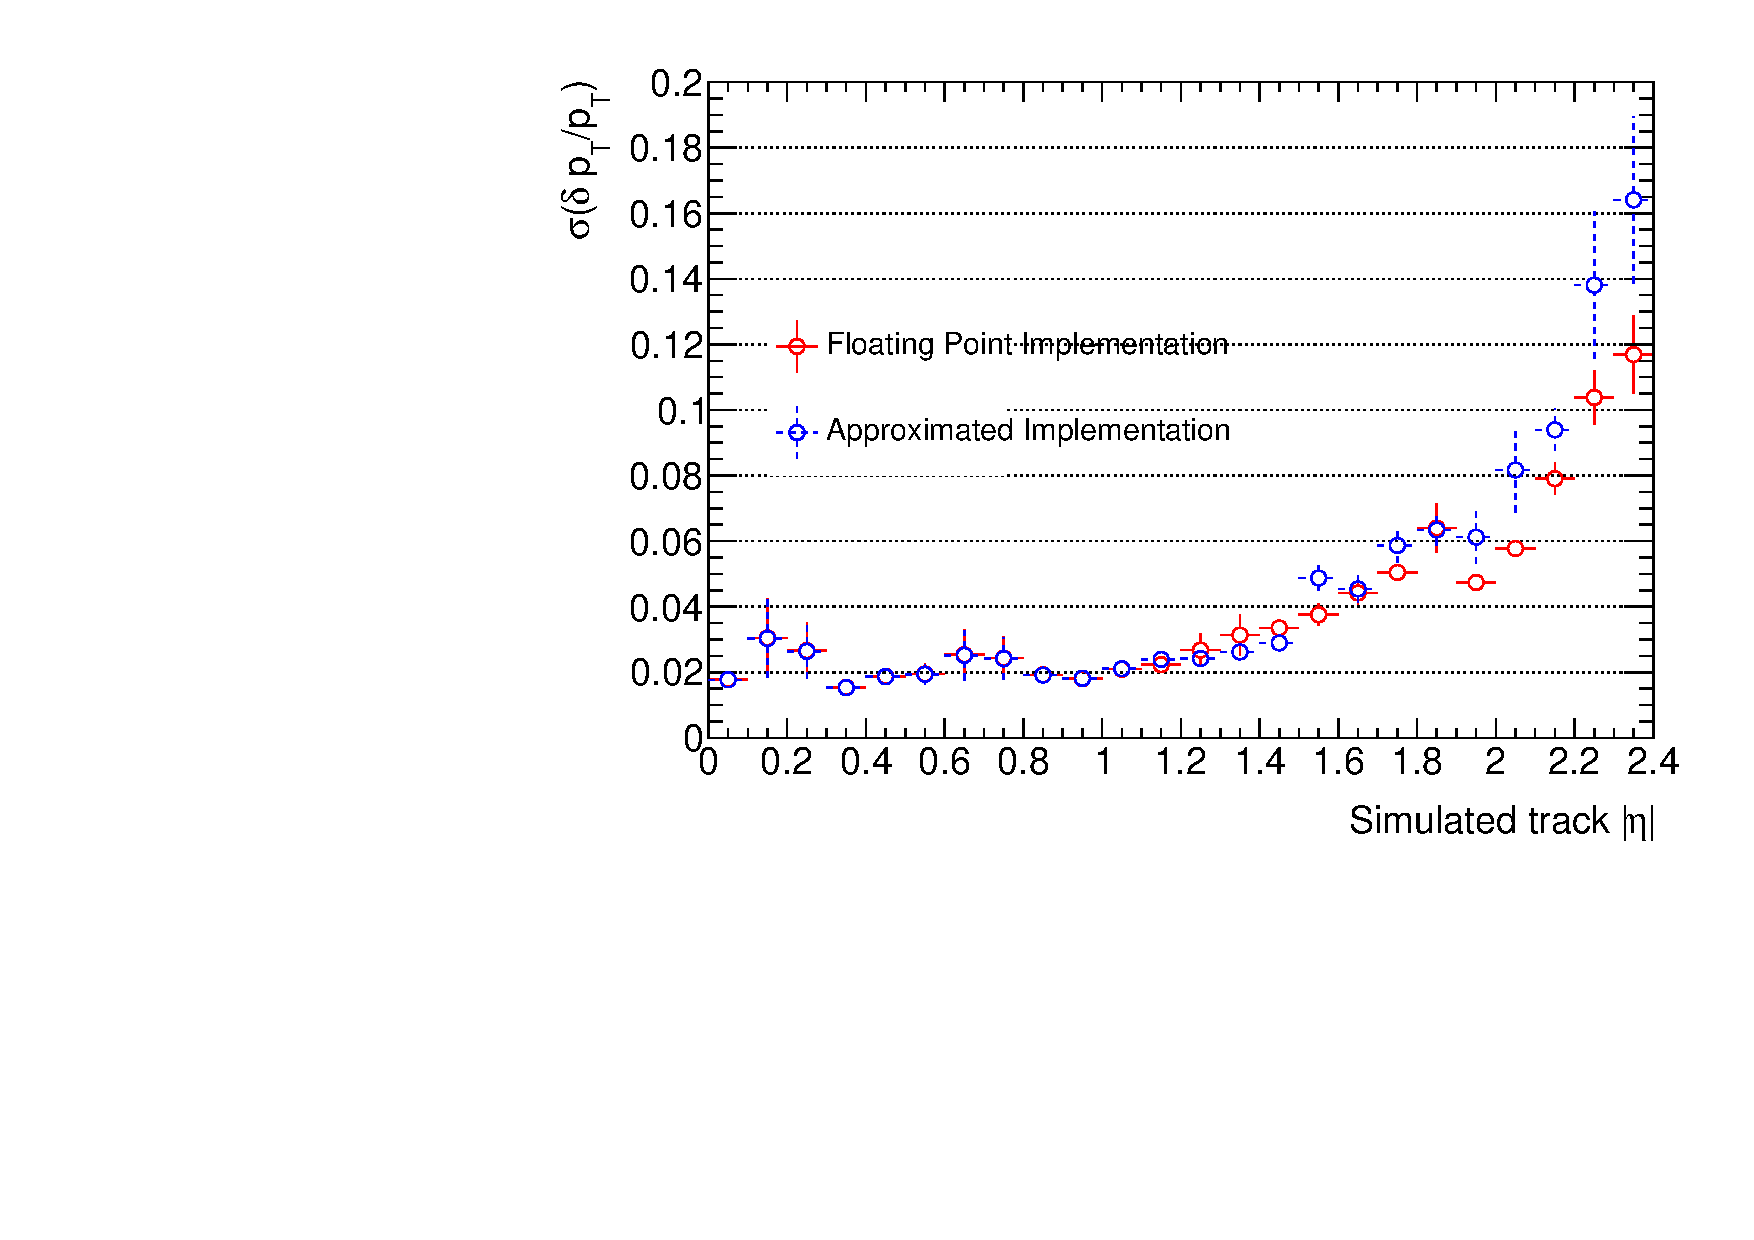
\includegraphics[width=0.49\textwidth]{figs/tk-upgrade/results-chi2fitter/ptRelResVsEta_It_1_ApproxVsExact.pdf}
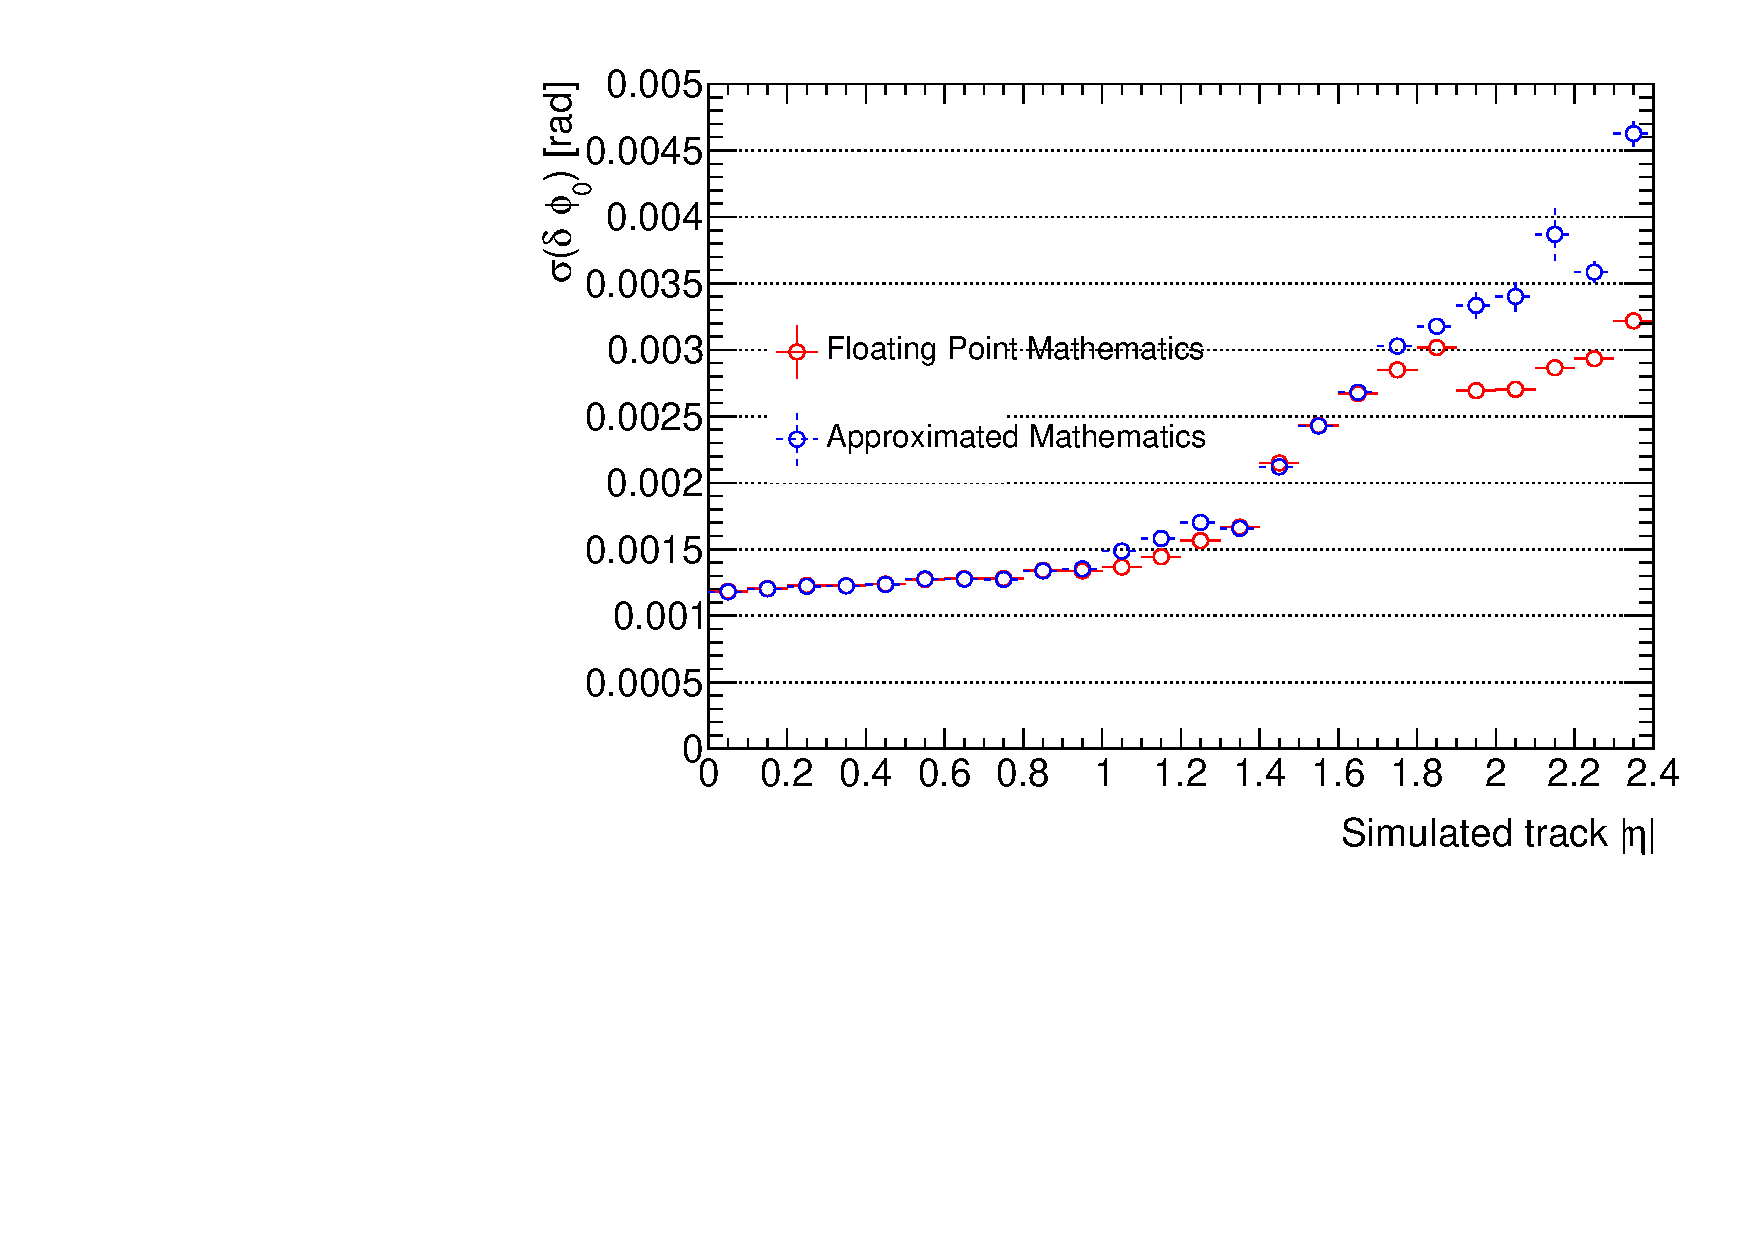
\includegraphics[width=0.49\textwidth]{figs/tk-upgrade/results-chi2fitter/phi0ResVsEta_It_1_ApproxVsExact.pdf}
\\
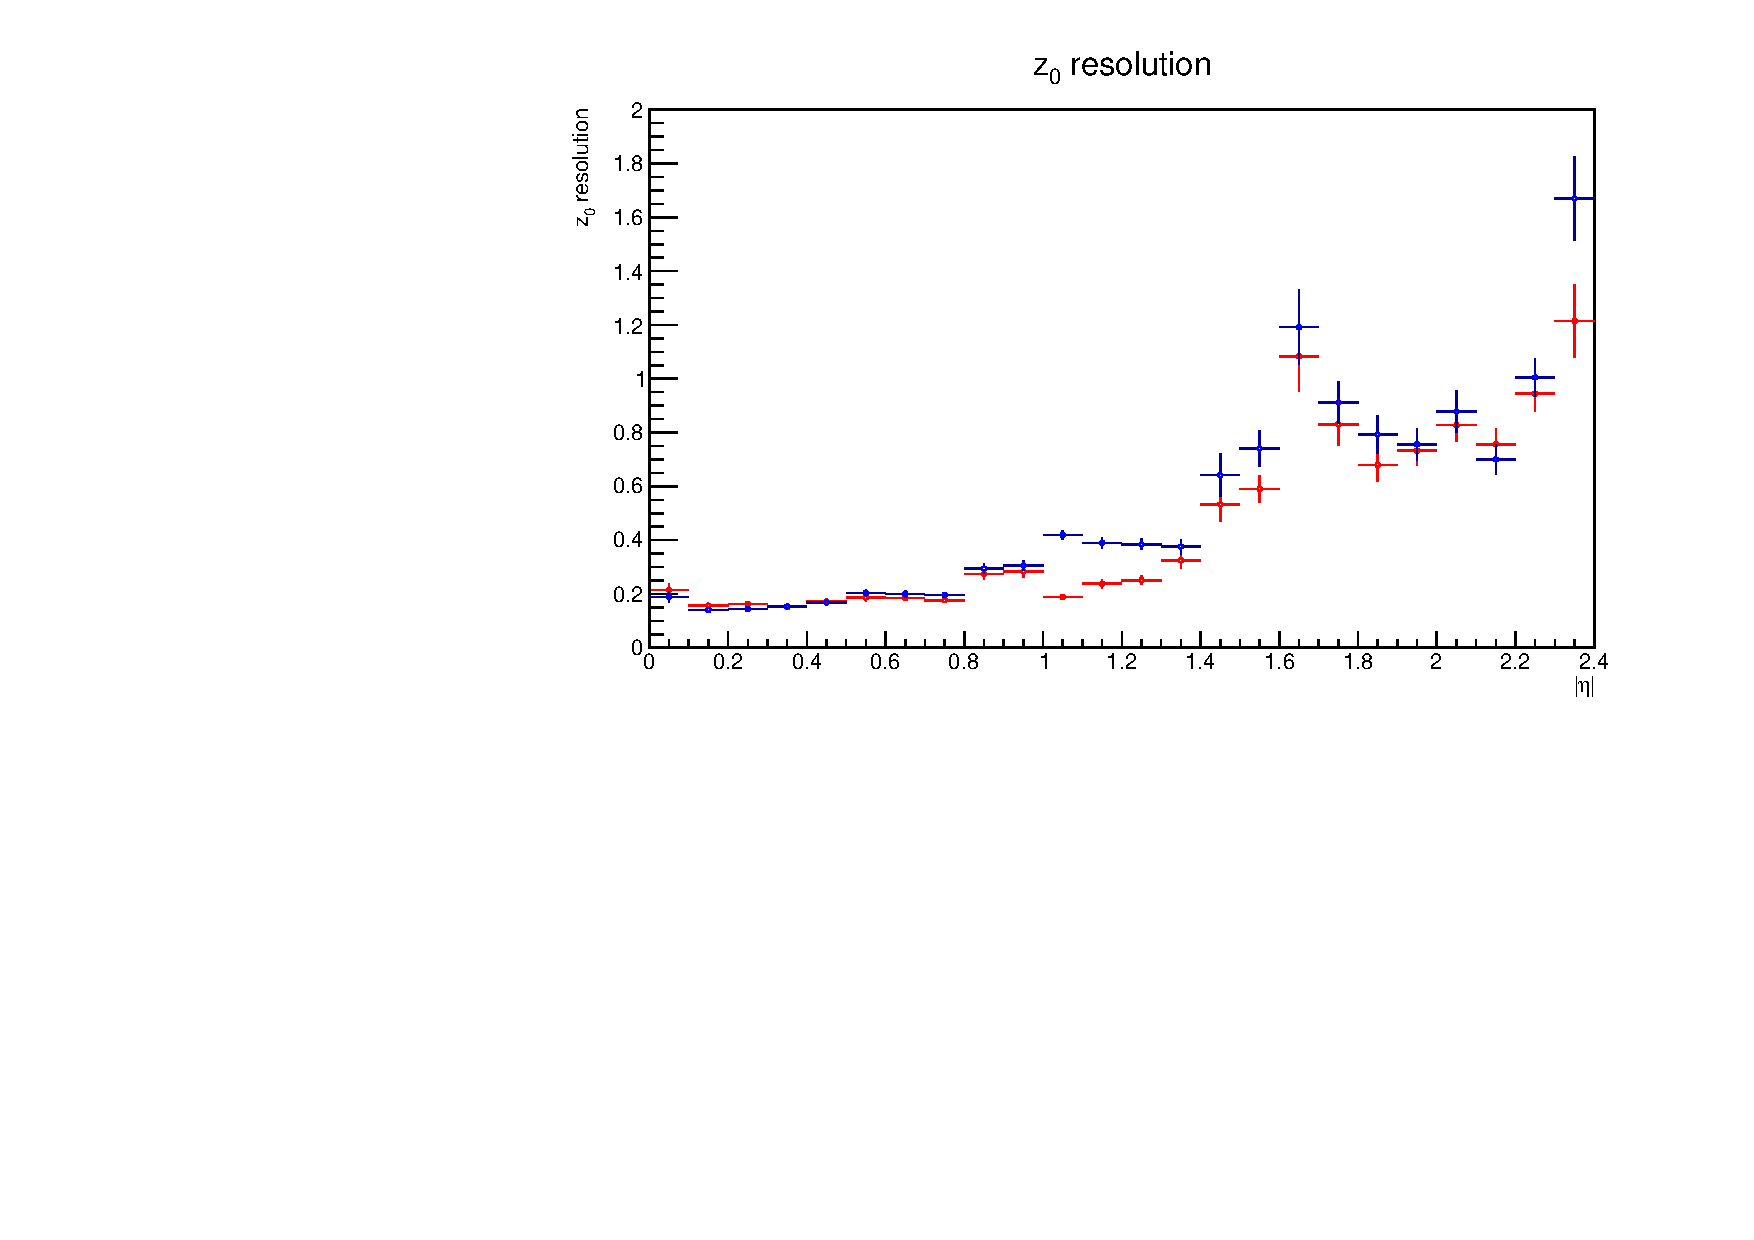
\includegraphics[width=0.49\textwidth]{figs/tk-upgrade/results-chi2fitter/z0ResVsEta_It_1_ApproxVsExact.pdf}
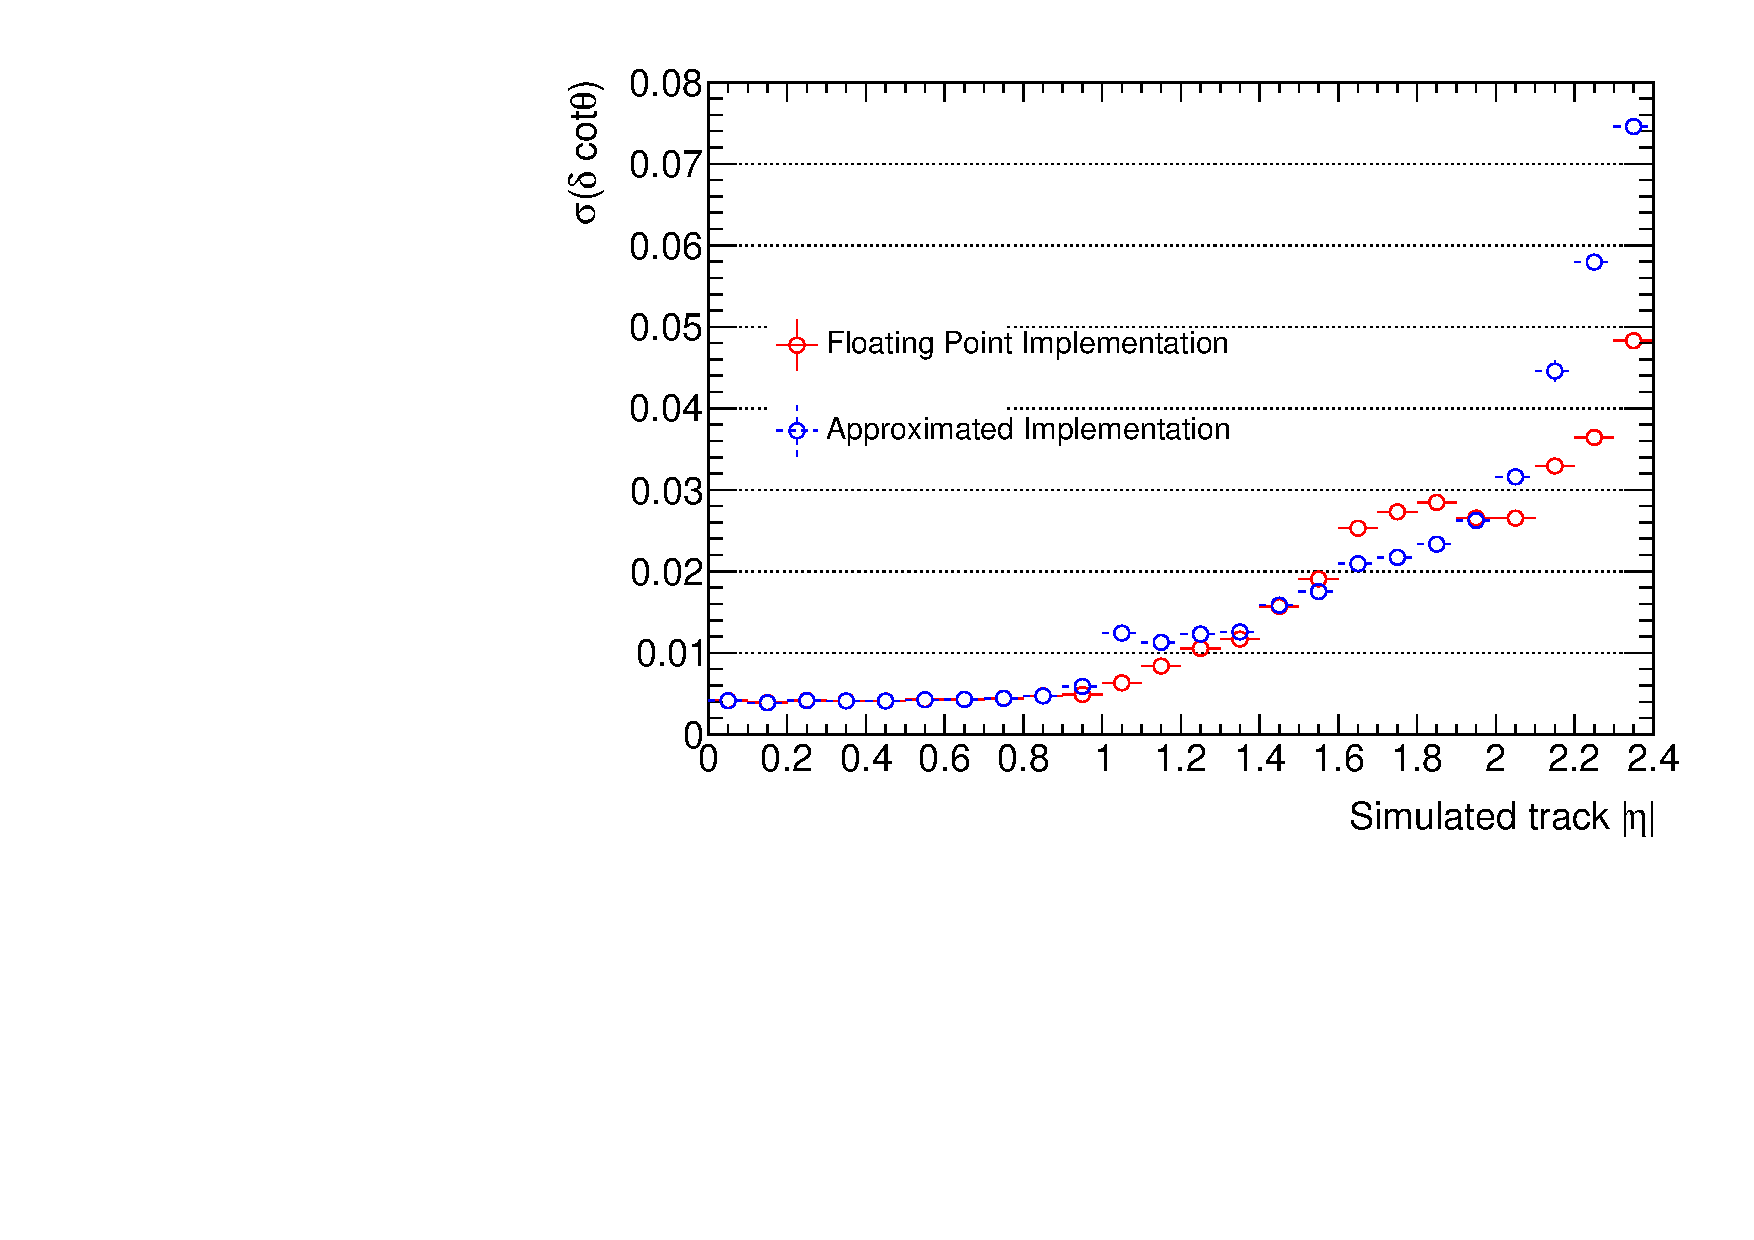
\includegraphics[width=0.49\textwidth]{figs/tk-upgrade/results-chi2fitter/cotThetaResVsEta_It_1_ApproxVsExact.pdf}
\caption{
Distributions of \pt relative resolution, $\phi$ resolution, $z_{0}$ resolution and $cot(\theta)$ resolution measured for primary reconstructed tracks in simulated \ttbar events with a <PU> of 200 for the floating point (red) and approximated maths (blue) implementations of the linearised $\chi^{2}$ fit algorithm for a single fitting iteration.
\editComment{Make plots bigger!}
}
\label{fig:chi2HelixParametersResVsEtaApproxVsExact}
\end{figure}

%Running multiple iterations of the fitting algorithm had been previously been considered in the context of improving upon the resolution of a fitted track's helix parameters, but had been shown to produce only marginal improvements.

Figure~\ref{fig:chi2HelixParametersResVsEtaApproxVsExact} shows that resolutions of the four track parameters as a function of $\eta$ from primary tracks in \ttbar events at a <PU> of 200 for both mathematical implementations of the algorithm.
The resolutions compare well not just between the two implementations of the algorithm's mathematics, but also with those obtained for the barrel region with the offline track reconstruction which is able to use all information from the detector with more sophisticated reconstruction techniques ~\cite{P2TrackerTDR}.
While this guarantees that the tracks found in the the barrel will be useful to the L-1 trigger, the significant presence of at least one stub being incorrectly associated with a matched track in the forward regions, as shown in Table~\ref{tab:chi2-exactVsApprox}, significantly degrades the resolution obtained.

In order to filter out these incorrectly assigned stubs from matched tracks, and also remove fake tracks, the residuals calculated for each stub following the fit were considered.
These ``fake'' stubs are expected have large residuals compared to stubs correctly associated to genuine tracks or stubs belonging to a fake track.

Therefore, in order to decrease the fake rate and increase tge  matched track purity:
\begin{itemize}
\item the stub with the worst/largest residual is found;
\item this stub is compared against a configurable threshold;
\item the stub is removed from the track if its residual exceeds the threshold value;
\item the track is refitted using only its remaining stubs;
\item and the process is repeated until the latency budget is exceeded/no further stubs are removed, with no further consideration of the remaining stubs' residuals following the final threshold.
\end{itemize}

During the optimisation of this stub quality check it was found that a track could end up having fewer than the minimum of four stubs required to be considered track candidate - thus potentially discarding a matched track by mistake.
To avoid this while still retaining the improved matched track purity and reduced fake rate, a looser residual threshold was applied for tracks only containing four stubs.

\begin{table}[htbp]
\topcaption {Track finding performance on simulated \ttbar events at a <PU> of 200, for the $\chi^{2}$ track fit using approximated calculations of the track derivatives for when one to four fitting iterations are undertaken. 
Further fitting iterations are not shown as further improvement was observed.
}
\label{tab:chi2_iterations}
  \centering
% This increases column spacing.
  \resizebox{\textwidth}{!}{
% This right-aligns numbers in column, but centers them under column title.
 \begin{tabular}{ccccccc}
   \hline
   \bf{Track Fitter} & [\#] of iterations & \bf{$\bm{\epsilon}$ [\%]} & \bf{$\bm{\epsilon_{P}}$ [\%]} & $\bm{<N_{tracks}$ & \bf{Fakes [\%]} & \bf{Duplicates [\%]}  \\
   \hline
   $\chi^{2}$+DR & 1 & 94.9 & 85.6 & 87.4 & 15.5 & 10.9 \\  
   & 2 & 93.8 & 91.0 & 73.8 & 6.6 & 7.7 \\
   & 3 & 93.1 & 91.0 & 71.4 & 5.3 & 6.9 \\
   & 4 & 93.0 & 91.0 & 71.1 & 5.2 & 6.8 \\
   \hline
   KF+DR & - & 94.1 & 94.1 & 82.1 & 21.1 & 4.5 \\
   \hline
   
 \end{tabular}}
\end{table}

Table~\ref{tab:chi2_iterations} illustrates how the tracking performance of the linearised $\chi^{2}$ fitter improves with just one additional fitting iteration (removal of a stub), with the fake rate halving and matched track purity noticeably improving, albeit at the expense of the looser definition of the track finding efficiency.
Further successive fitting iterations yield diminishing returns, with no further improvements seen following four fitting iterations.
Given that the mean number of hits associated to a track is seven, the majority of tracks can only have up to three stubs removed.
By contrast, while a greater number of fake tracks survive the \KF's filtering, the \KF achieves a similar tracking efficiency as two iterations of the $\chi^{2}$ fitter while none of the matched tracks found contain any incorrect stubs. 
This suggests that if a more sophisticated method of removing bad quality stubs were used in the linearised $\chi^{2}$ fitter, then  not many matched tracks would be discarded while their purity would be increased.
Although such an improvement may come at the expense of a low fake rate, such tracks can be potentially cleaned further downstream but tracks which aren't reconstructed are lost forever.

Figure~\ref{fig:chi2HelixParametersResIterationsComparison} shows helix parameter resolution differences between one and four fitting iterations of the $\chi^{2}$ fitter, allowing for the removal of zero and up to three stubs respectively, and how this compares against the \KF's performance.
The additional fitting iterations allow for noticeable improvements for the track parameter resolutions obtained in the forward regions.
While the \qpt and $\phi_{0}$ resolutions achieved after four fitting iterations is comparable to those achieved by the \KF, the $\chi^{2}$ fitter's resolution is considerably worse for both the $z_{0}$ and $cot(\theta)$ resolutions in the endcaps.

\begin{figure}[htb]
\centering
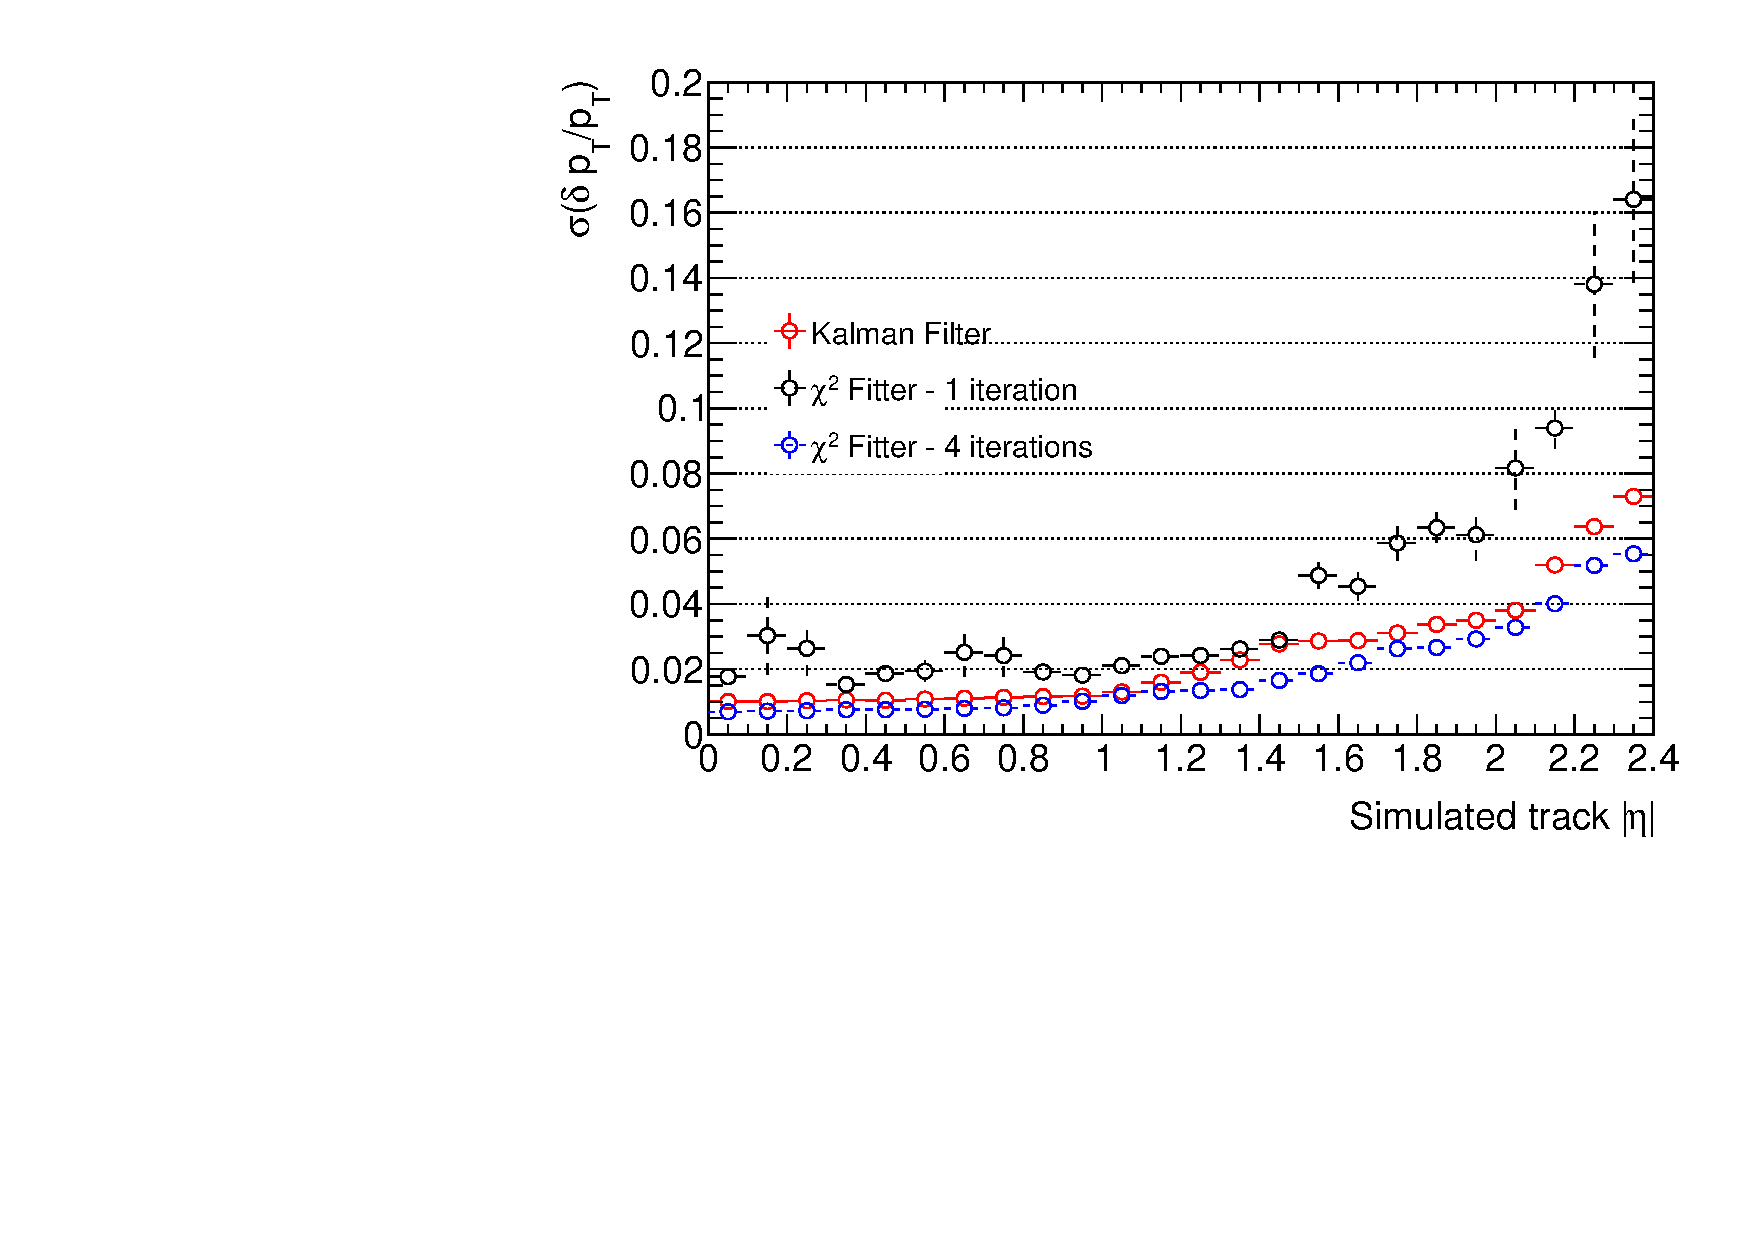
\includegraphics[width=0.49\textwidth]{figs/tk-upgrade/results-chi2fitter/ptRelResVsEta_IterationComparison.pdf}
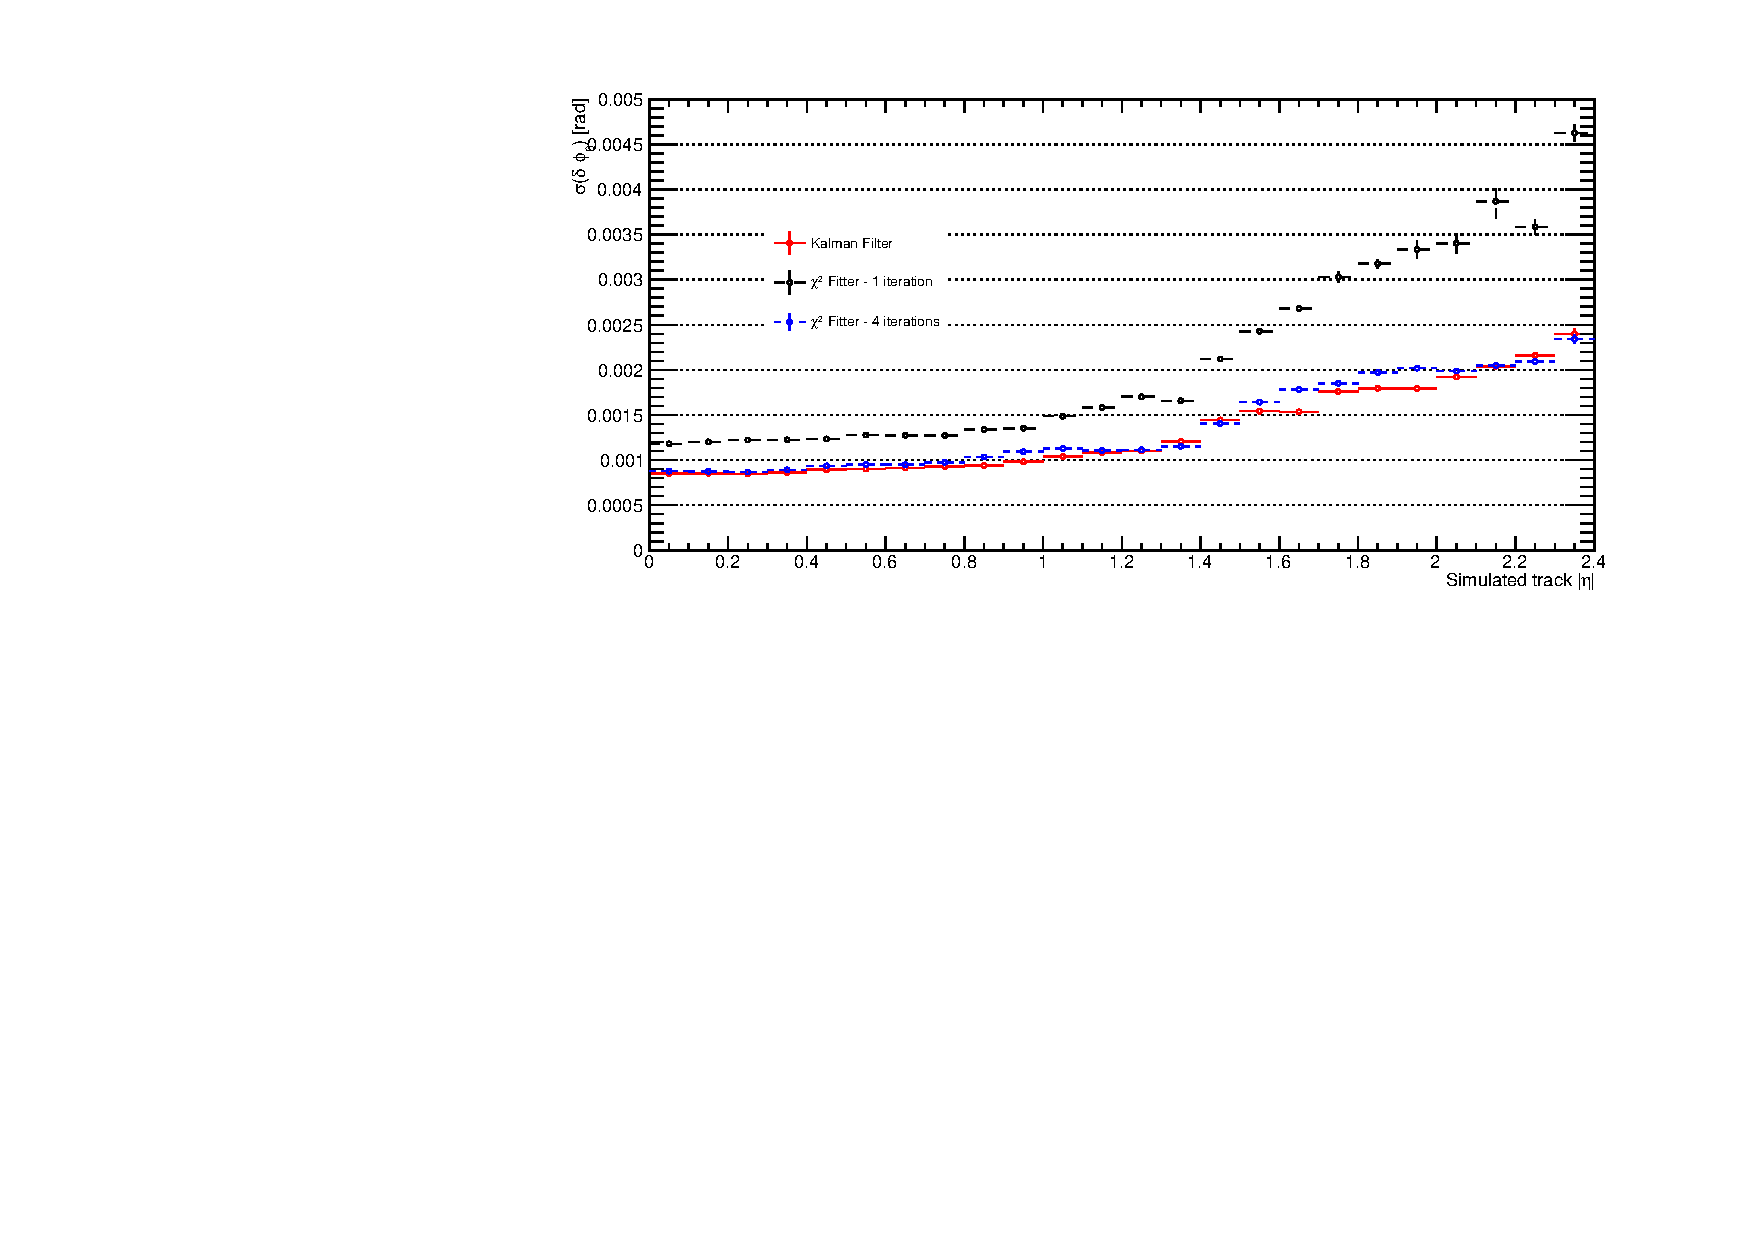
\includegraphics[width=0.49\textwidth]{figs/tk-upgrade/results-chi2fitter/phi0ResVsEta_IterationComparison.pdf}
\\
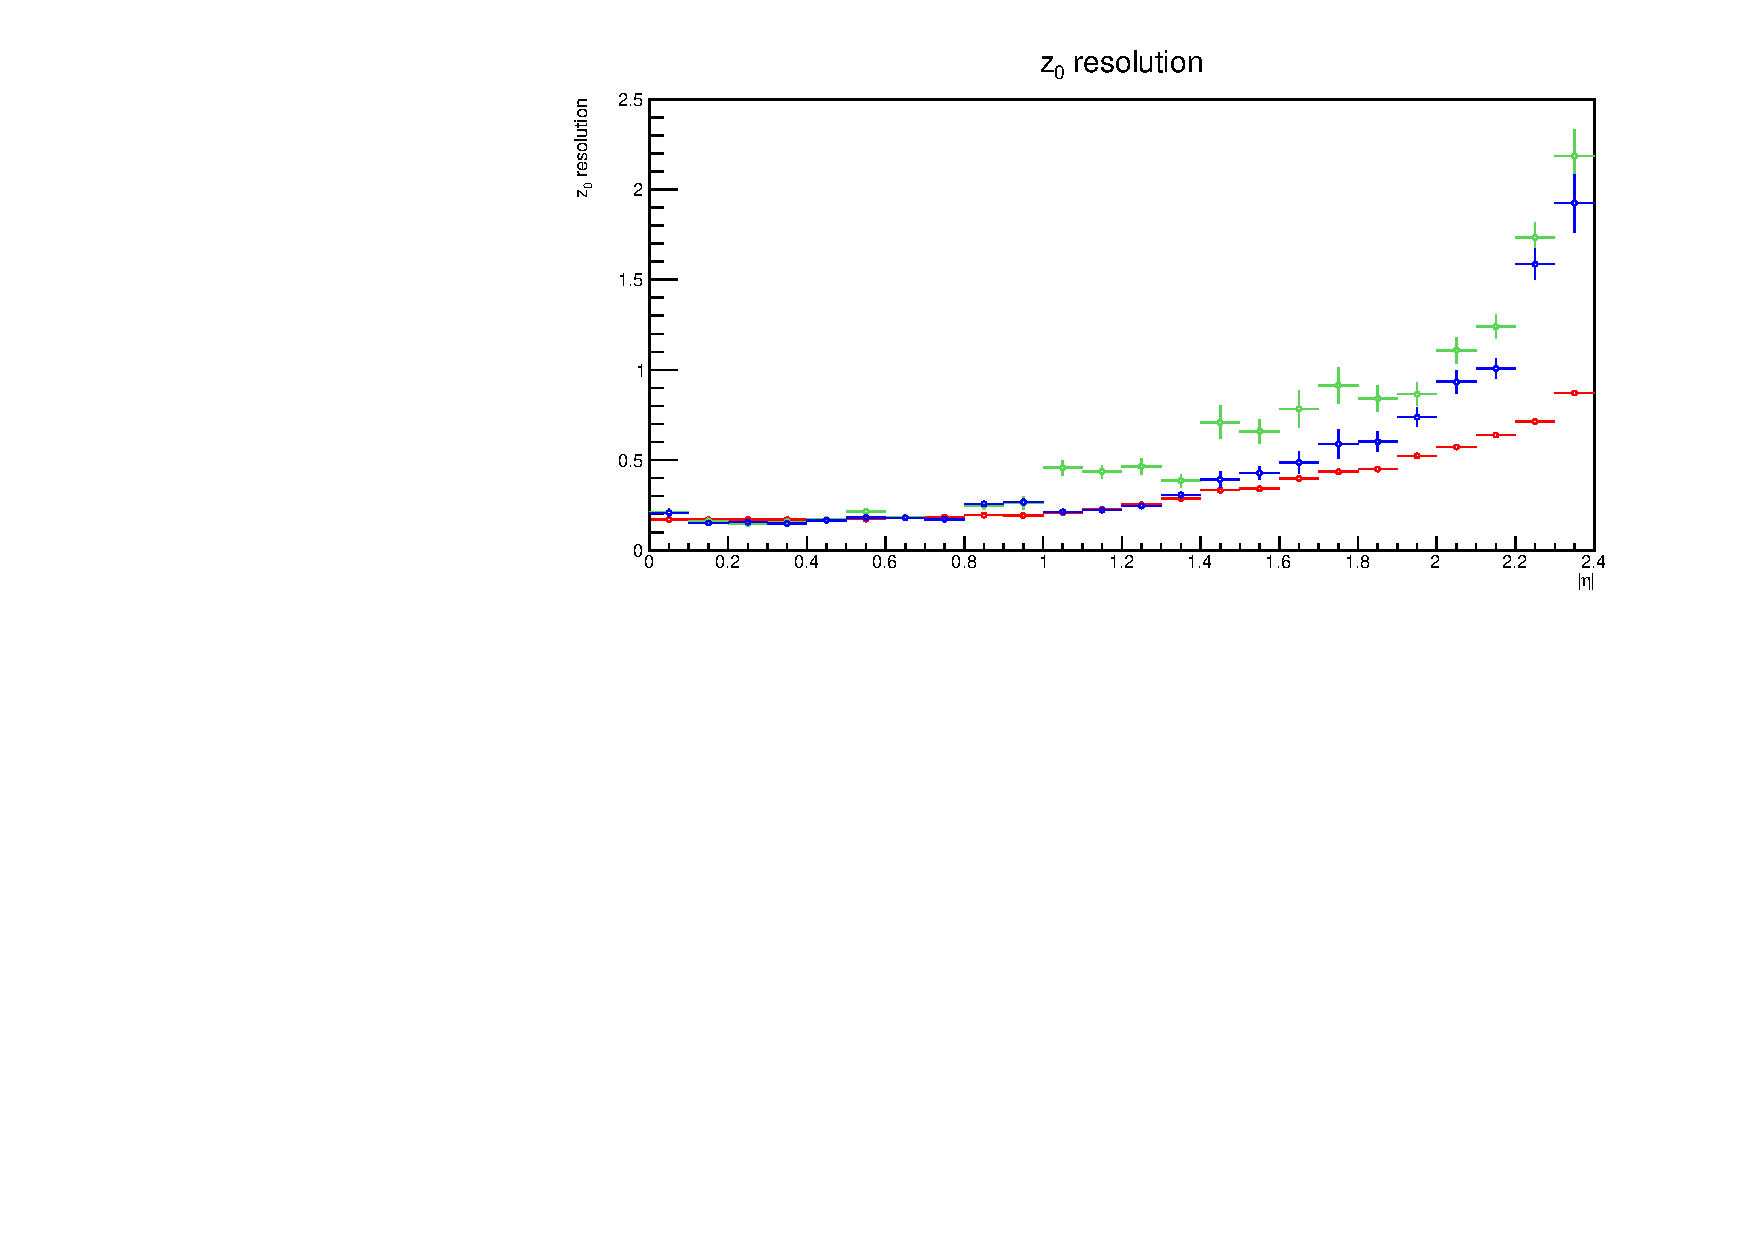
\includegraphics[width=0.49\textwidth]{figs/tk-upgrade/results-chi2fitter/z0ResVsEta_IterationComparison.pdf}
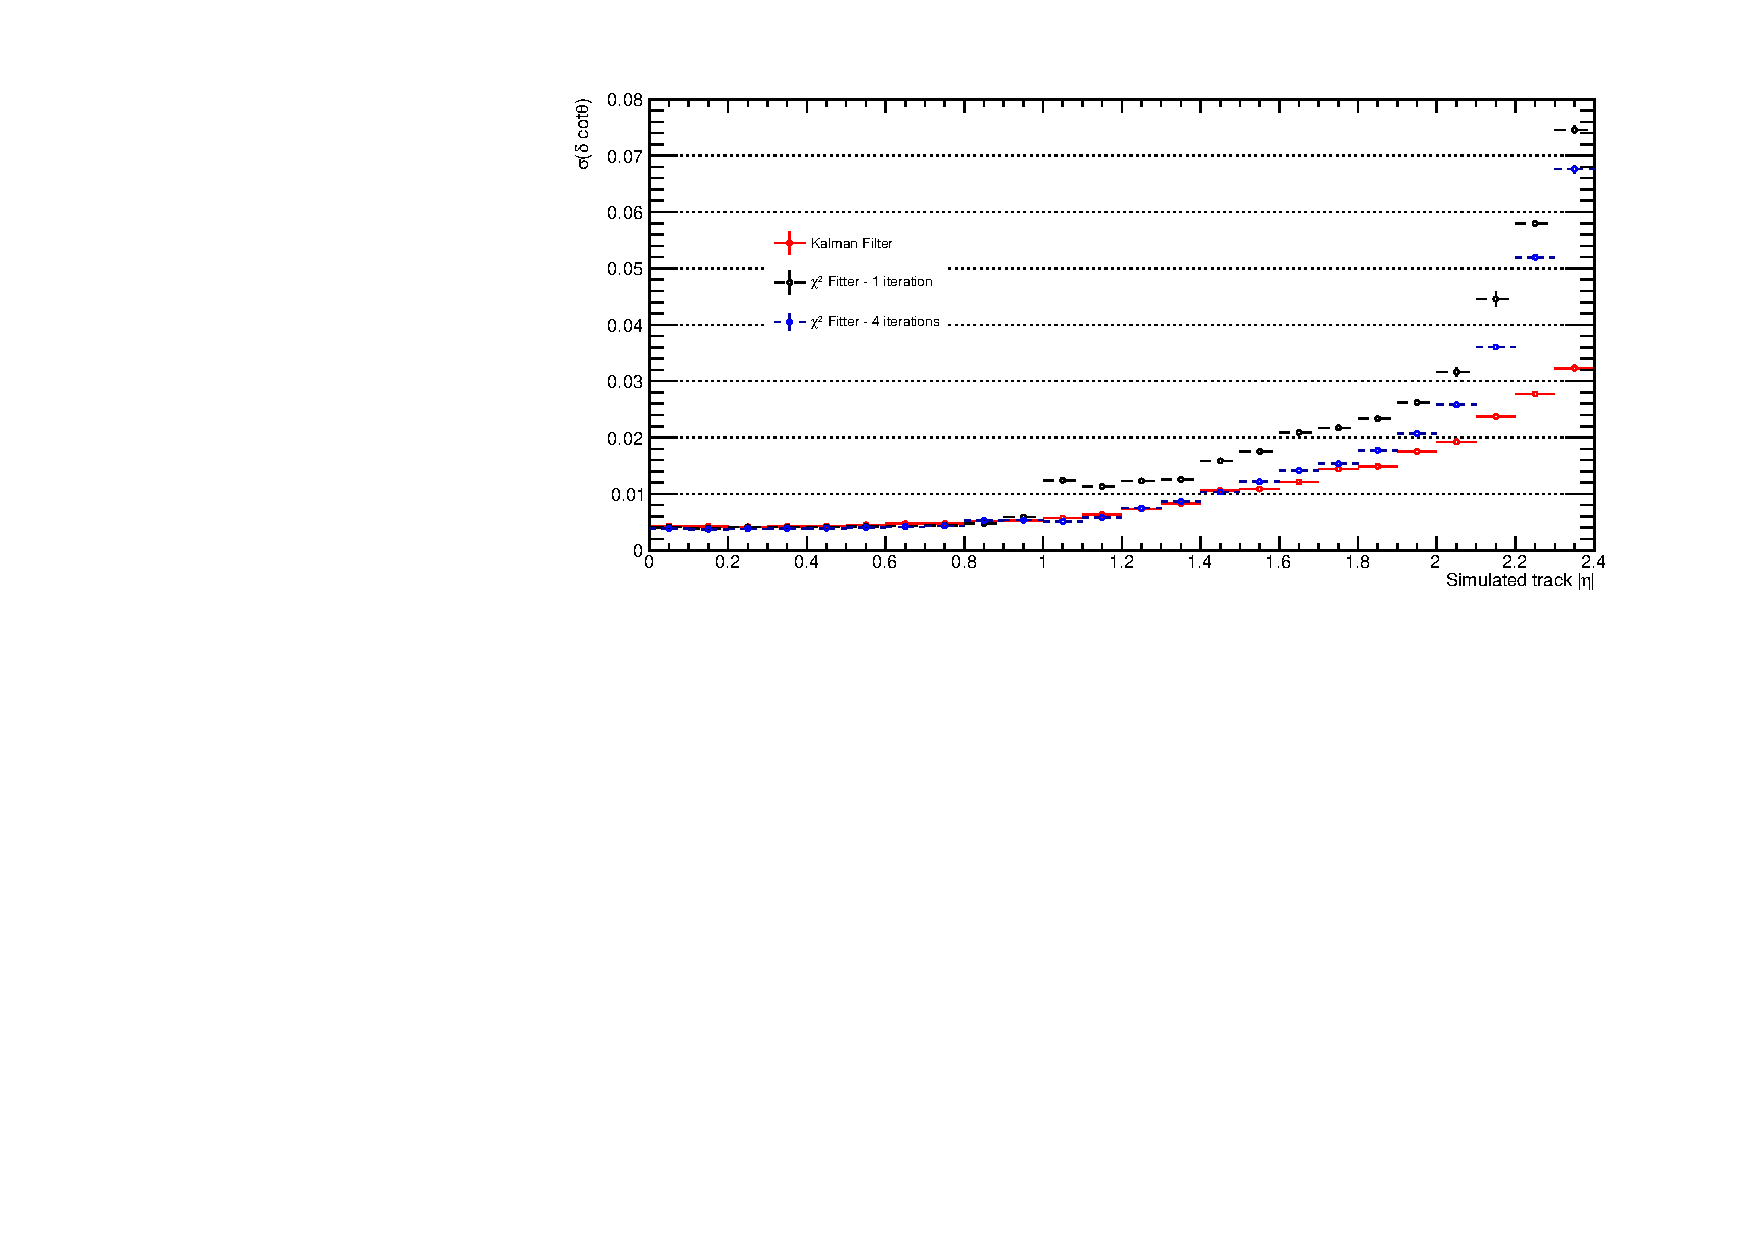
\includegraphics[width=0.49\textwidth]{figs/tk-upgrade/results-chi2fitter/cotThetaResVsEta_IterationComparison.pdf}
\caption{
\pt relative resolution, $\phi$ resolution, $z_{0}$ resolution and $cot(\theta)$ resolution measured for primary reconstructed tracks in simulated \ttbar events at a <PU> of 200 for the approximated maths implementation of the linearised $\chi^{2}$ fit algorithm for one (black) and four (blue) fitting iterations. The \KF (red) is also included for comparison.
\editComment{Make plots bigger!}
}
\label{fig:chi2HelixParametersResIterationsComparison}
\end{figure}

Following the parallel development of both the linearised $\chi^{2}$ track fit and the \KF however, it was decided that development of the former would be discontinued.
The reason behind this decision were that the \KF was capable of achieving a higher track finding efficiency with 100.0\% purity for matched tracks and $z_{0}$ and $cot(\theta)$ resolutions in the forward regions that were comparable to the expected offline resolution.
Considerable progress had also been made with an implementation in firmware.

In contrast, the linearised $\chi^{2}$ track was not competitive in terms of track resolution and reconstruction ability, especially with respect to the stricter tracking efficiency definition.
There were also concerns over the potential feasibility of tabulating all (or the most frequently used) track derivatives in the endcap disks for FPGAs that were commercially available at the time.

\subsection{Tracking at low transverse momentum}\label{subsec:Tmtt2GeV}
The flexibility to reconstruct tracks down to a lower \pT threshold of 2\GeV is potentially desirable and so the impact of this potential requirement on the performance of the proposed track-finder system was studied.

These studies were initially undertaken as part of the the robustness studies required for the 2016 demonstrator review, focussing on recovering tracking efficiency below 3\GeV with the \HT.
Therefore, the results for these studies were produced using the flat barrel geometry.

Following the 2016 review, the studies into tracking with a pT threshold of 2\GeV 
The initial studies were subsequently developed with modifications to the \KF algorithm after 2016.

The results for the \KF improvements were produced with the preferred tilted barrel geometry.



As the number and width of \qpt \HT columns used varies from the standard fixed number and size of columns typically used, thus varying the \pT resolution available, the track parameters are expressed as a function of 1/\pT instead of \pT.

\subsubsection{Hough Transform Optimisation}\label{subsubsec:lowPtOptHT}
Lowering the \pT threshold from 2\GeVc required modifying the GP and HT configuration parameters to ensure adequate duplication in $\phi$ and increasing the number of \qpt columns by 50\% to take into account the increased \pt range whilst maintaining the same precision.
The increased number of \qpt columns increases the required FPGA resources by 50\% and the output data rate from the \HT by a factor of 2.2.

Without applying further modifications, there is a considerable degradation in the track reconstruction efficiency in the range $2\GeVc < \pt < 2.7\GeVc$, due to these low momenta tracks being dominated by multiple scattering.
This results in a significant fraction of stubs not intersecting within a single \HT cell and thus failing to exceed the threshold criteria and generate track candidates.
To mitigate against such track reconstruction efficiency losses, using a preexisting feature which had been separately implemented in firmware, the precision of the \HT cells along \qpt and $\phi_{T}$ for the range $2\GeVc < \pt < 2.7\GeVc$ was reduced by a factor of two (\ie $2 \times 2$ cells were merged).
Additionally, the \KF state $\chi^2$ cuts for this low \pT range were optimised to reflect the increased hit position uncertainty resulting from the decreased precision of the hits in these \HT cells and thus reduce the number of duplicate and fake tracks as far as possible without impacting on the \HT track reconstruction efficiency.
Figure~\ref{fig:2GeVFlatEff} shows how the tracking efficiency improves following the use of the variable precision \HT with and without optimised \KF state cuts after both the \HT and the full demonstrator chain. 

\begin{figure}[tbp]
\centering
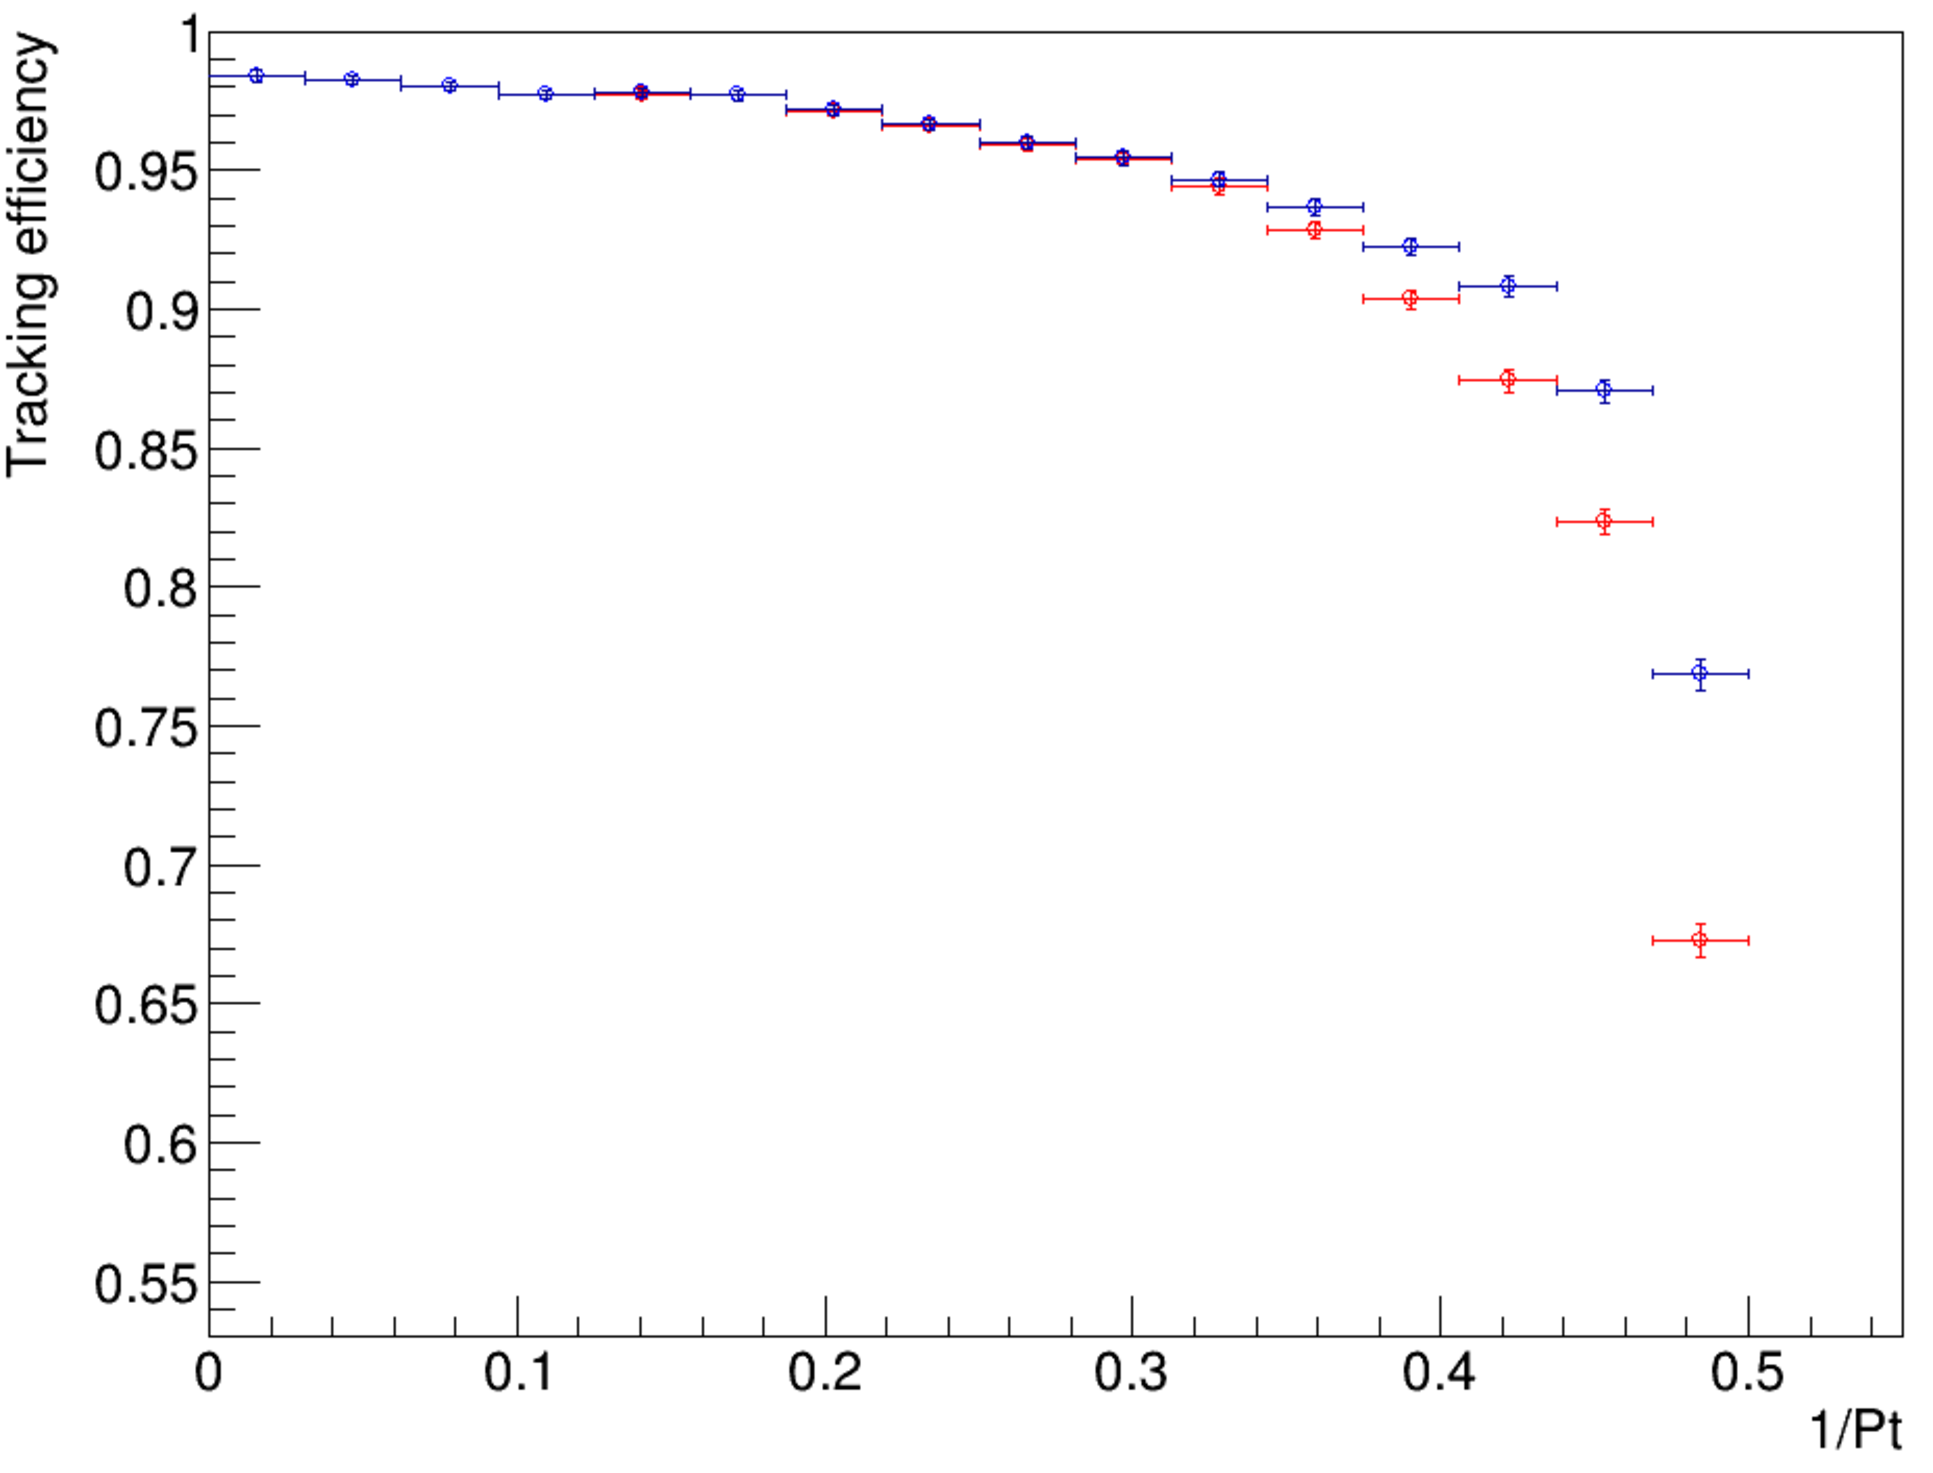
\includegraphics[width=0.49\textwidth]{figs/tk-upgrade/results-lowPtTracking/htTrackingEffVsInvPtFlatGeometry_5000.pdf}
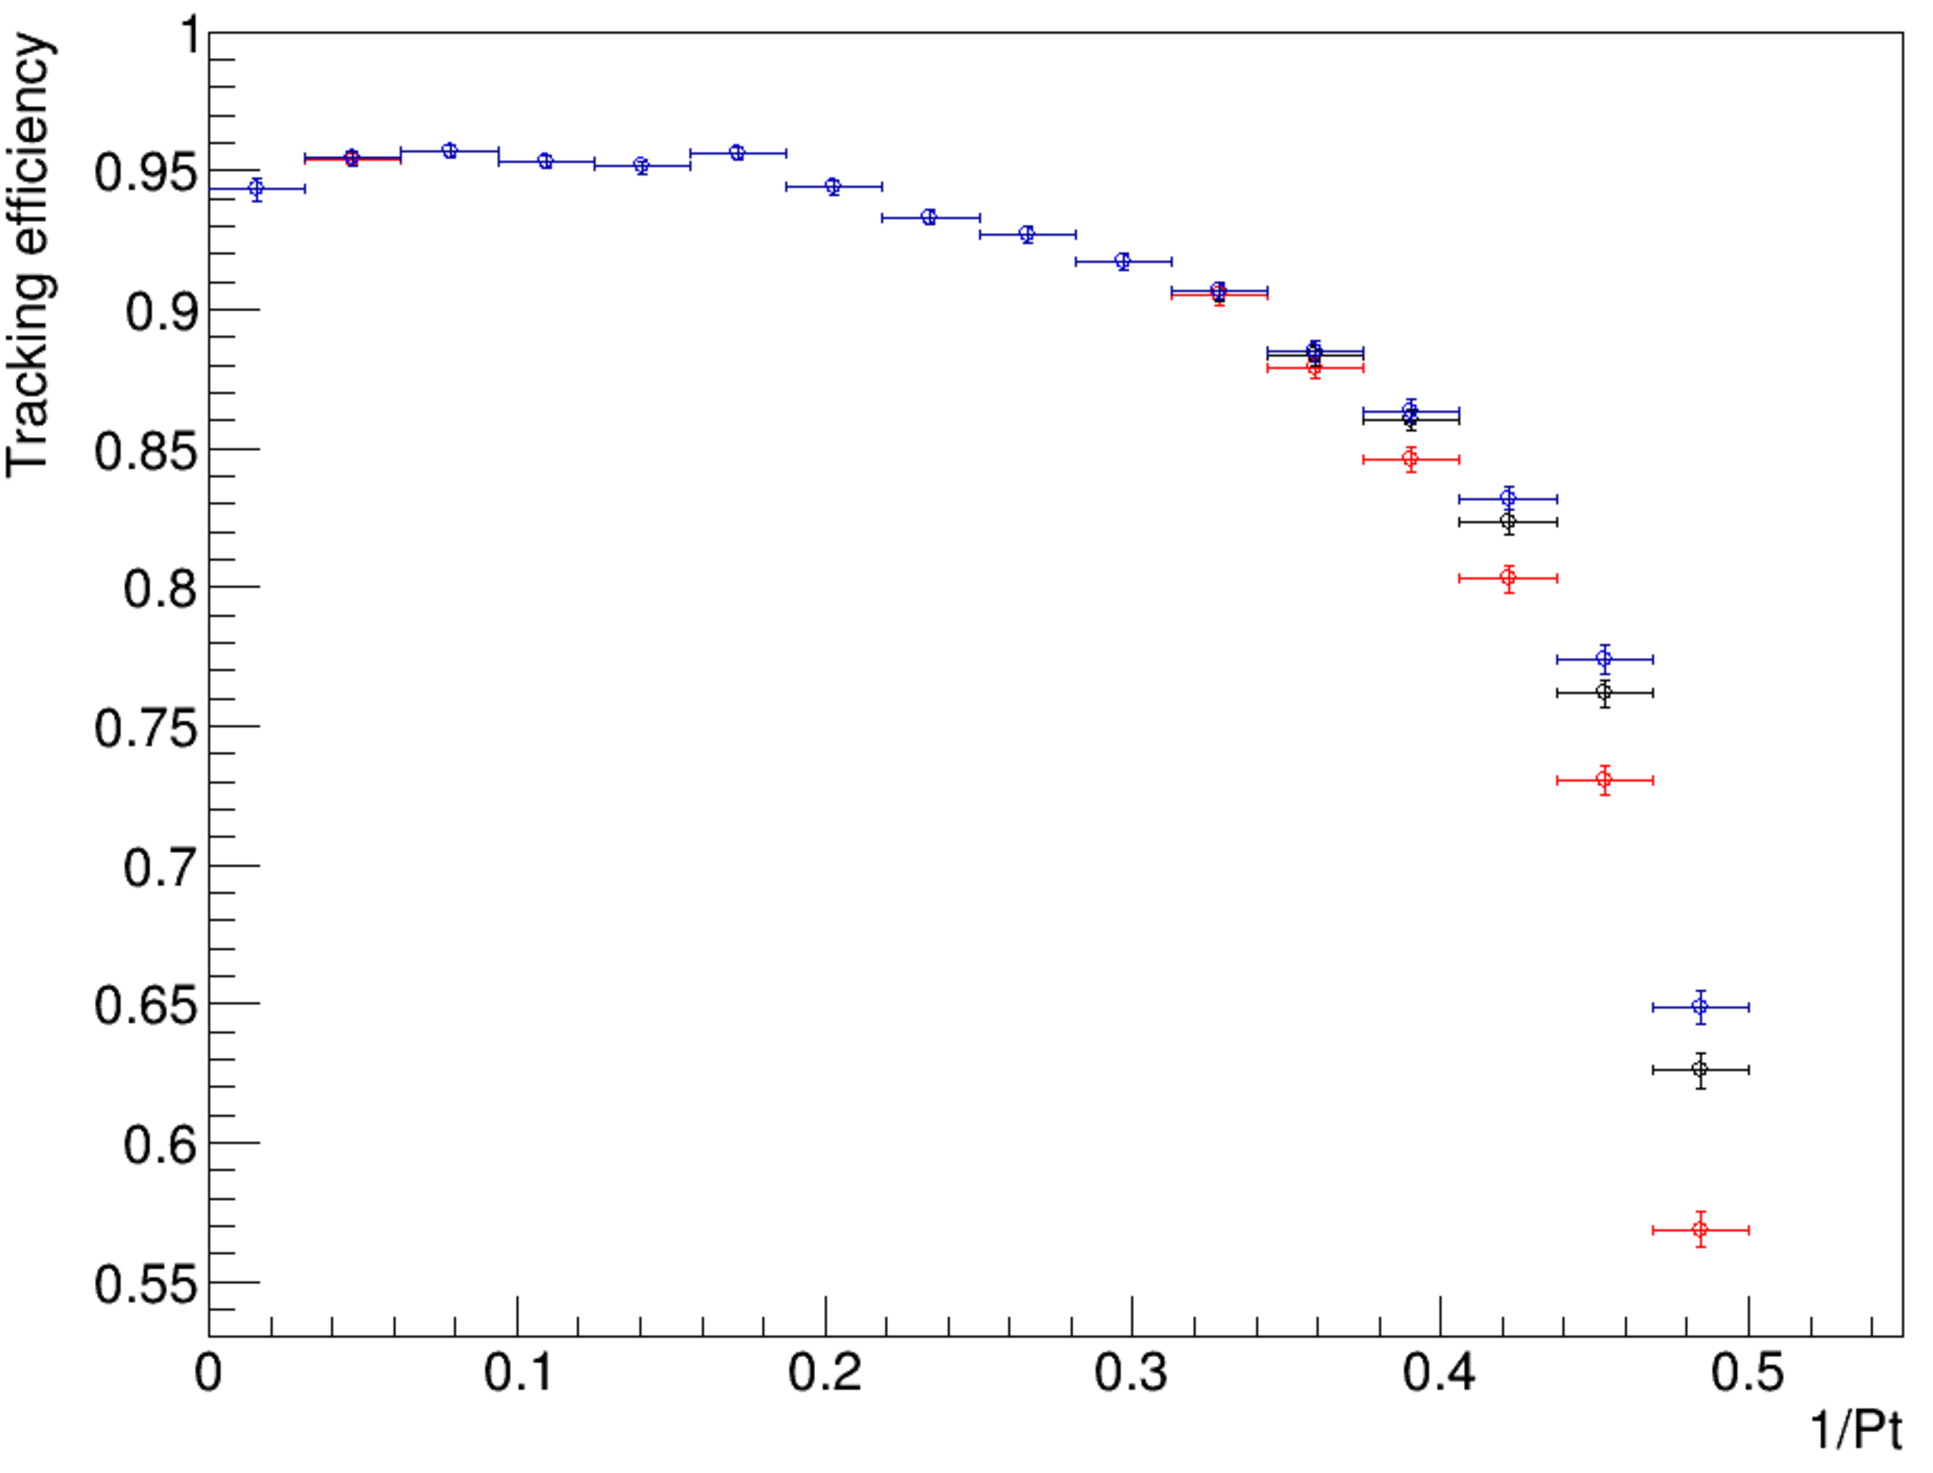
\includegraphics[width=0.49\textwidth]{figs/tk-upgrade/results-lowPtTracking/kfTrackingEffVsInvPtFlatGeometry_5000.pdf}
\caption{The post-\HT (left) and post-\KF (right) tracking efficiency for $\pt > 2\GeVc$ for \ttbar events at a <PU> of 200, with the default configuration where only the number of \qpt columns are increased (red) and with the increased number of columns, HT cell merging and \KF state cuts optimisation(blue).
}
\label{fig:2GeVFlatEff}	
\end{figure}

%%% Disucss table here
Table~\ref{tab:trackFindingPerformance2GeVHT} shows the impact that the decreased precision \HT cells and optimised \KF state cuts have on tracking performance both following the \HT and the full chain.
It is clear that whilst the merging of adjacent \HT cells recovers  tracks which did not previously intersect within a single \HT cell, the tracking efficiency following the full chain is significantly less than that post-\HT.
As shown in figure~\ref{fig:2GeVFlatEff}, these losses occur for tracks where the particle's transverse momentum is less than 3\GeV, as the \KF does not take the effects of \MS into account.
This shortcoming of the \KF also accounts for it not being as efficient at removing fake tracks, with an observed increase of 5\% in the fraction of fakes reconstructed.
The duplicate removal algorithm however, remains effective at removing almost all the duplicates.

\begin{table}[htbp]
\topcaption {Track finding performance on simulated \ttbar events at a <PU> of 200, after the \HT and the full chain  for the configurations of only increasing the number of \qpt columns (\emph{Default}), additionally using \HT cell merging and the optimised \KF state cuts (\emph{Optimised}).
The track finding efficiencies following each stage are given using the efficiency definitions given in Section~\ref{subsec:helixParameter}, along with the mean number of tracks and the fraction of those tracks which are either fake or duplicate tracks.
\editComment{Fix table size}
}
\label{tab:trackFindingPerformance2GeVHT}
  \centering
% This increases column spacing.
  \resizebox{\textwidth}{!}{
% This right-aligns numbers in column, but centers them under column title.
\begin{tabular}{cccccc}
   \hline
   \bf{Configuration} & \bf{Stage} & \bf{Efficiency [\%]} & \bf{Mean \# of tracks} & \bf{Fakes [\%]} & \bf{Duplicates [\%]}  \\
        \hline
    Default & \bf{HT}     & 93.6 & 713.2 & 34.0 & 44.5 \\  
    & \bf{Full chain}     & 89.2 & 193.9 & 21.1 & 5.1 \\      
%   \hline
%    Merge & \bf{HT}     & 94.6 & 799.2 & 40.5 & 39.7 \\  
%    & \bf{Full chain}     & 89.8 & 206.5 & 25.4 & 3.9 \\      
    \hline
    Optimised & \bf{HT}     & 94.6 & 799.2 & 40.5 & 39.7 \\  
    & \bf{Full chain}     & 90.0 & 210.4 & 26.3 & 3.8 \\      
   \hline
   
 \end{tabular}}
\end{table}

The point made about \MS not being properly accounted for in the \KF is illustrated by figure~\ref{fig:2GeVFlatChi2Ndf} which shows the distributions of $\chi^{2}$ per number of degree of freedom ($\frac{\chi^{2}}{ndf}$) as a function of $\frac{1}{\pT}$ for genuine tracks produced by the \KF.
If all uncertainties were accounted for, the ideal distribution of $\frac{\chi^{2}}{ndf}$ would be unity for all \pT, in contrast to the dramatic increase above approximately 3\GeV from the approximately flat distribution at order unity.

\begin{figure}[tbp]
\centering
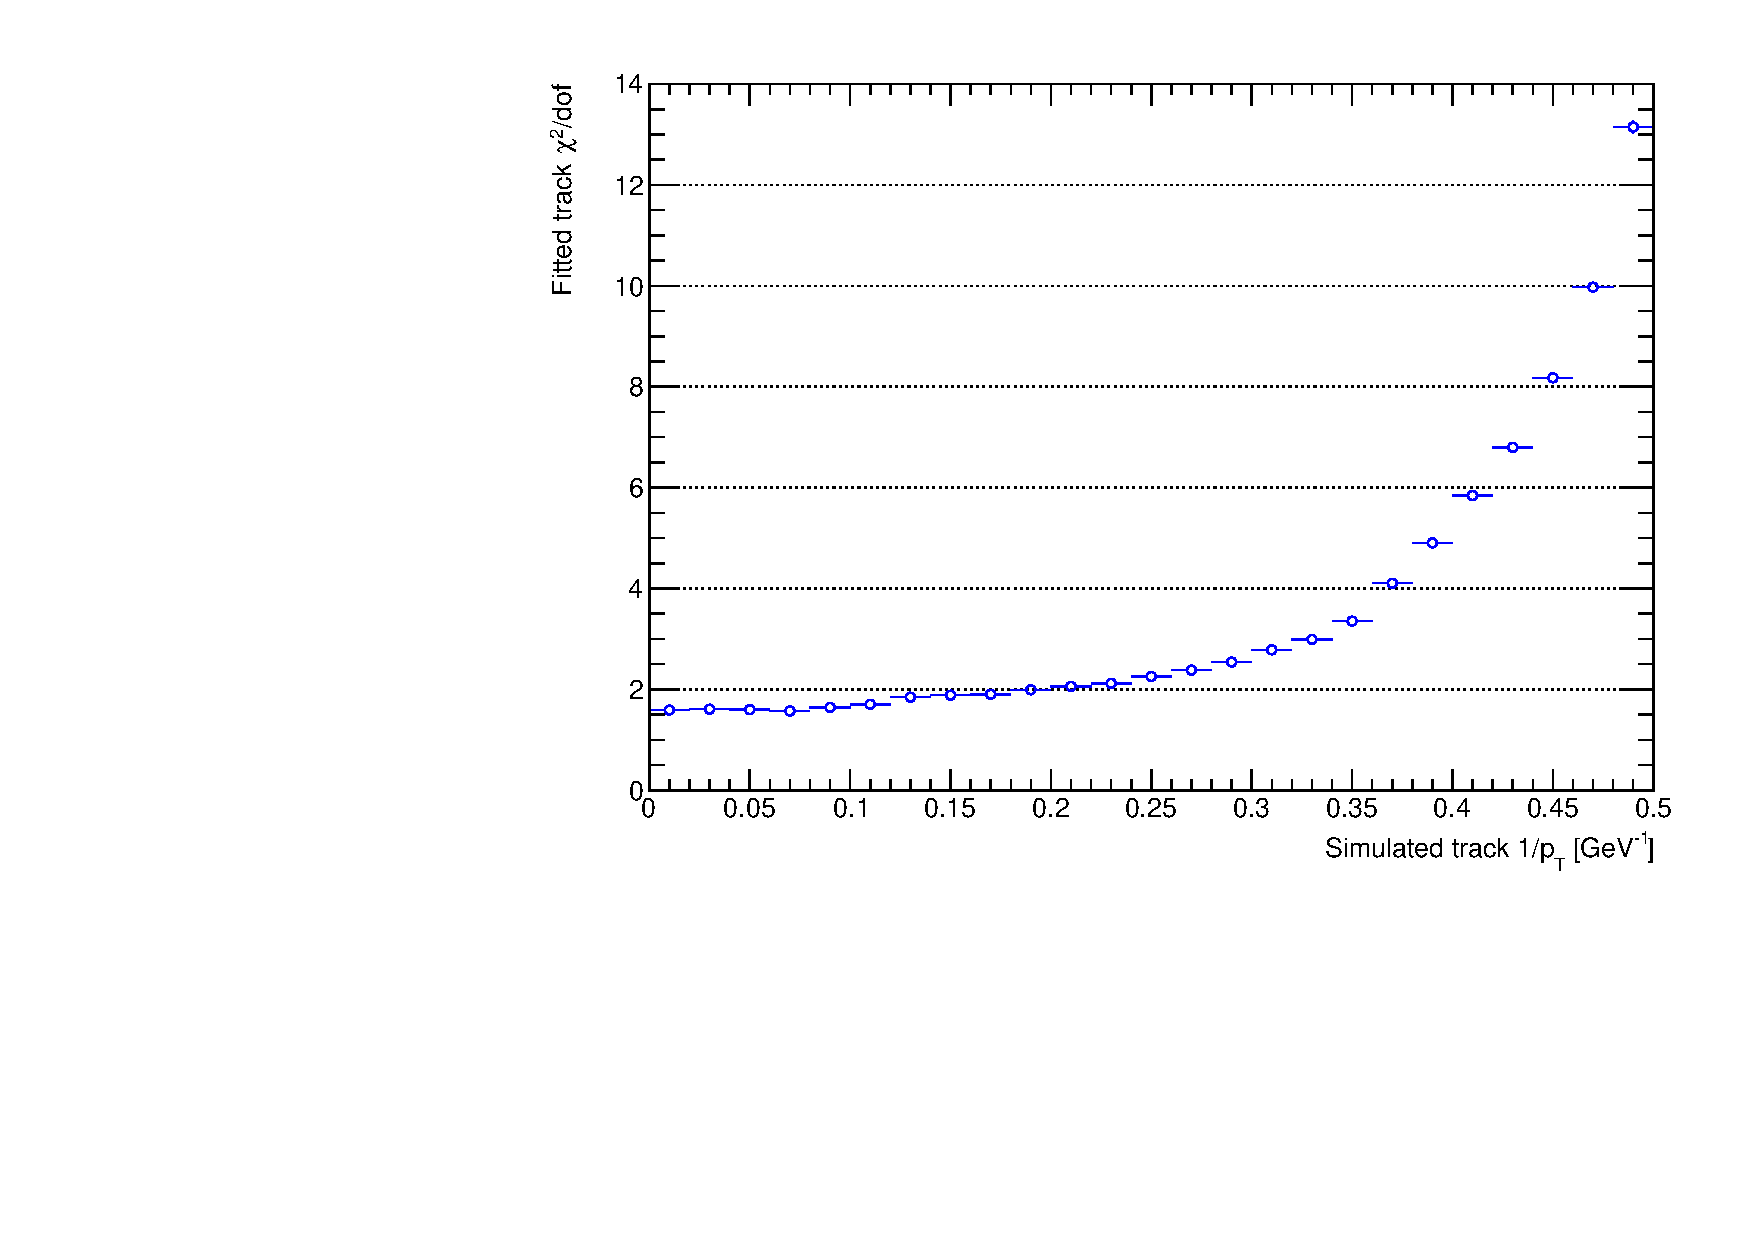
\includegraphics[width=\textwidth]{figs/tk-upgrade/results-lowPtTracking/kfChi2NdfVsInvPtFlatGeometry_5000.pdf}
\caption{Plot of $\frac{\chi^{2}}{ndf}$ as a function of $\frac{1}{\pT}$ for genuine tracks produced by the \KF.}
\label{fig:2GeVFlatChi2Ndf}
\end{figure}

%% Discuss the resolution plots here
Figure~\ref{fig:htHelixParametersResVsInvPt} shows that the resolutions of the track parameters fitted by the \KF are comparable for $\pT < 3\GeV$ for both the default configuration of the \HT where only the number of \qpt columns has been increased and after the \HT and associated \KF optimisations for tracks originating from the primary interaction in \ttbar events at a <PU> of 200.
The slight degradation in the $\phi_{0}$ resolution is a result of the decreased precision coordinates from the \HT and the small improvement observed in the $z_{0}$ resolution is due to the \KF being able to consider genuine stubs which were not previously found by the \HT.

\begin{figure}[htb]
\centering
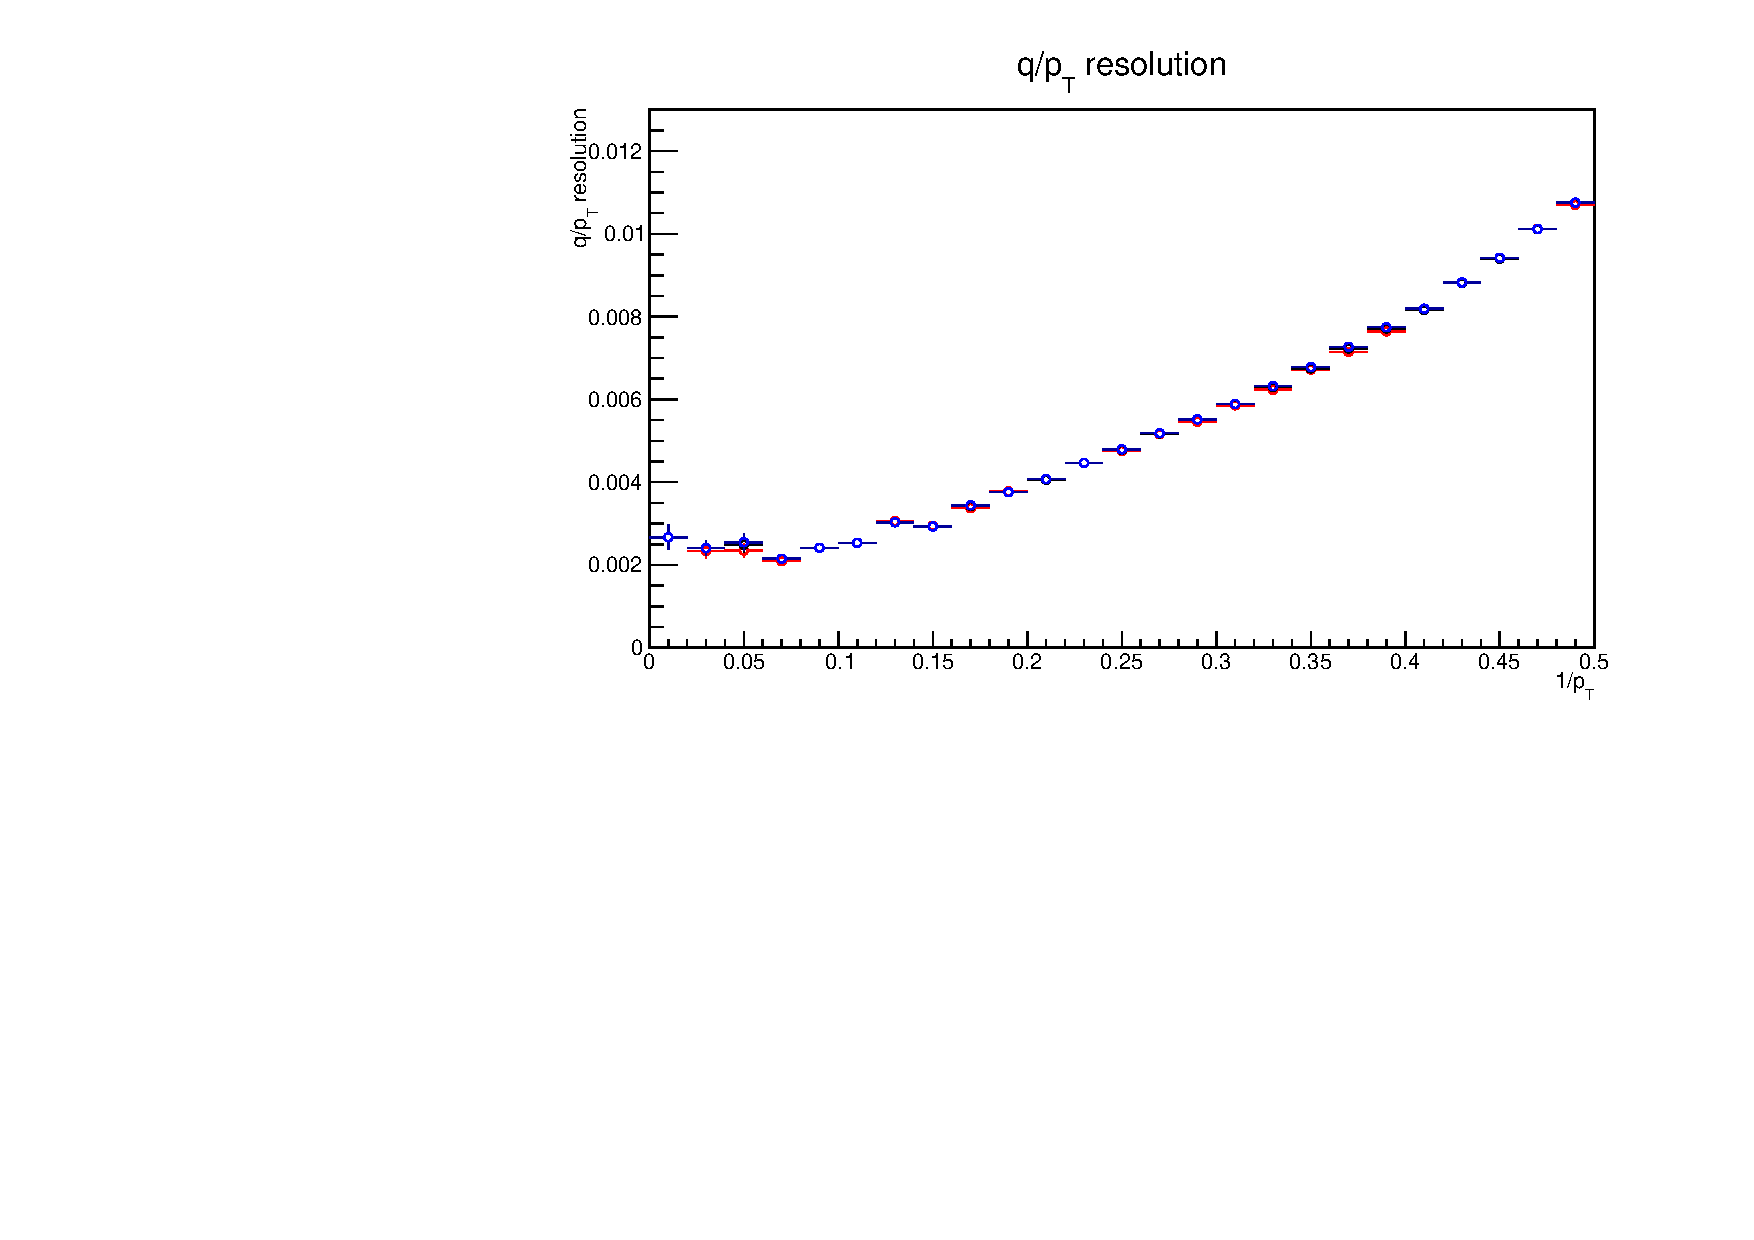
\includegraphics[width=0.49\textwidth]{figs/tk-upgrade/results-lowPtTracking/qOverPtResVsInvPtFlatGeometry_5000.pdf}
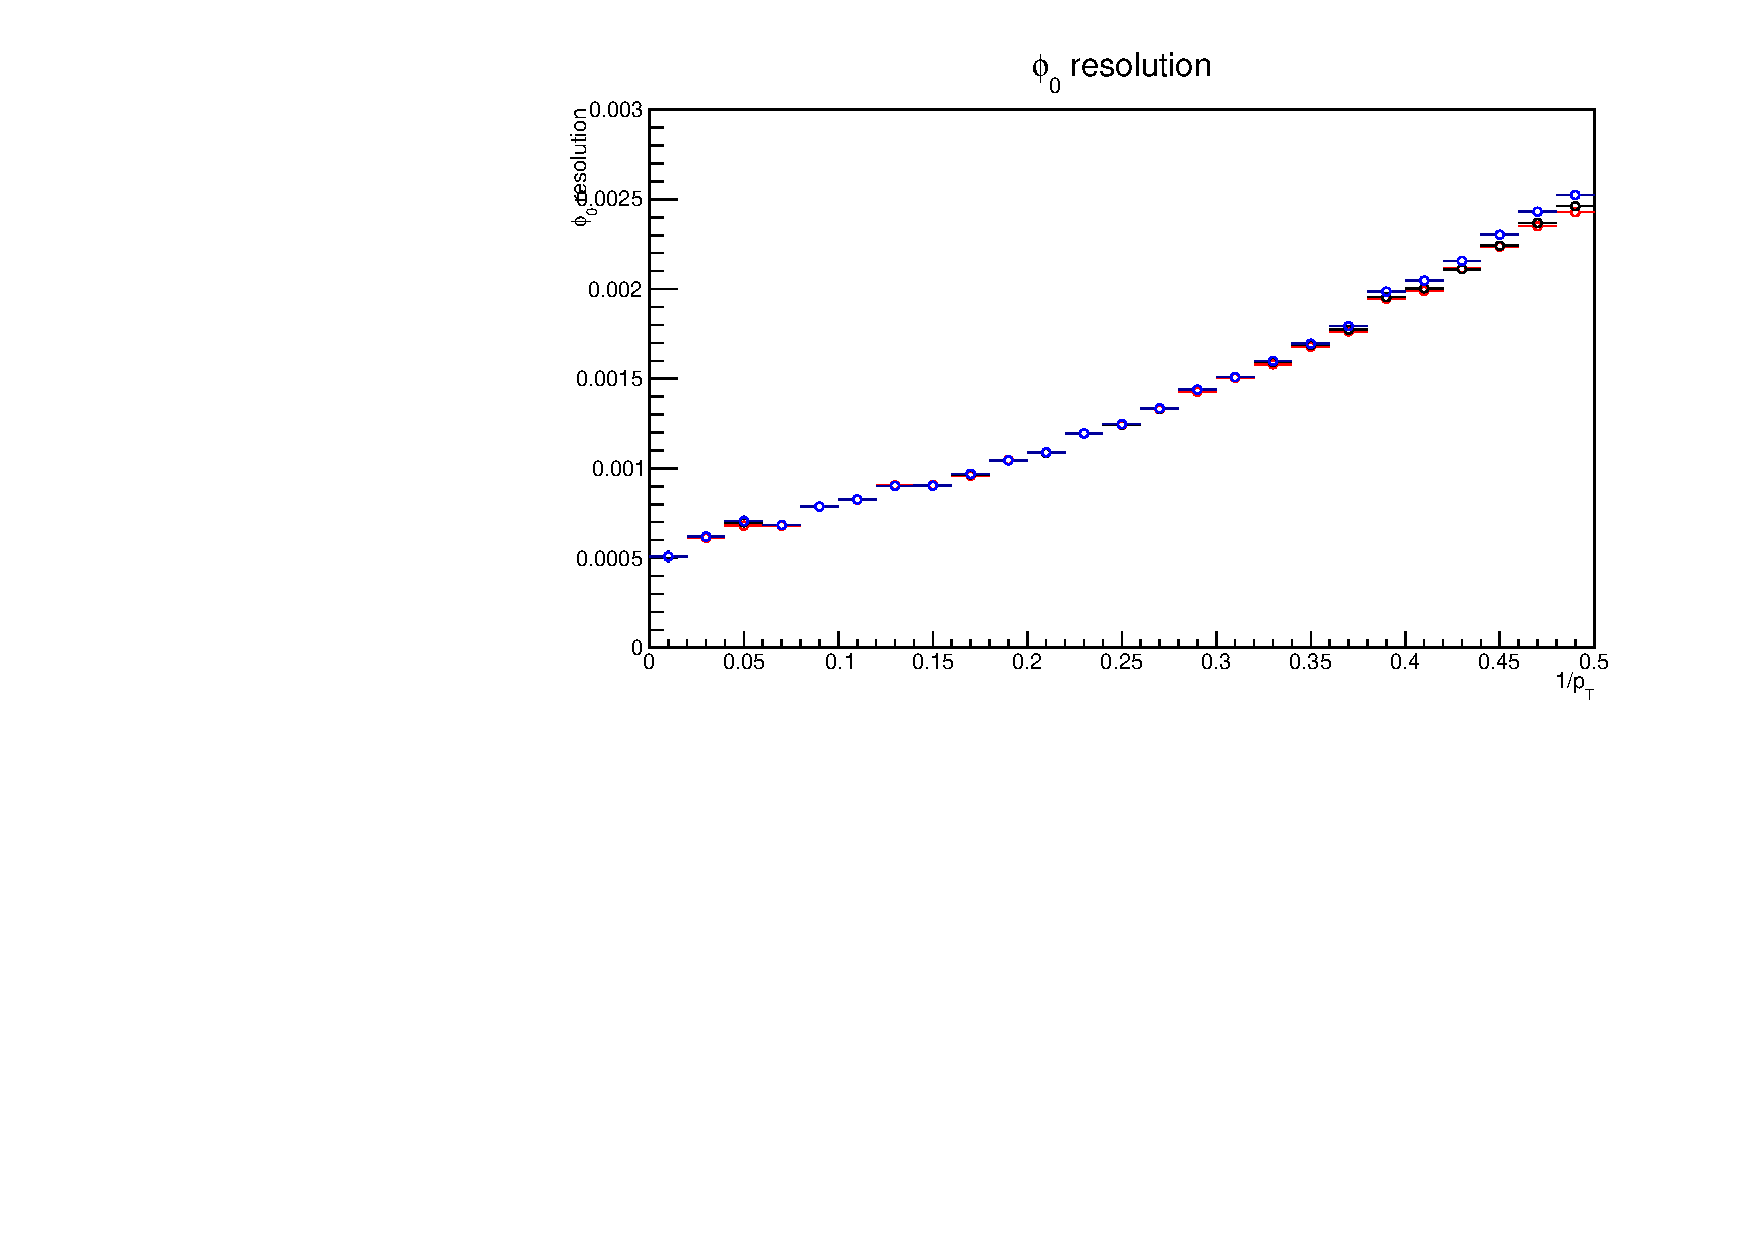
\includegraphics[width=0.49\textwidth]{figs/tk-upgrade/results-lowPtTracking/phi0ResVsInvPtFlatGeometry_5000.pdf}
\\
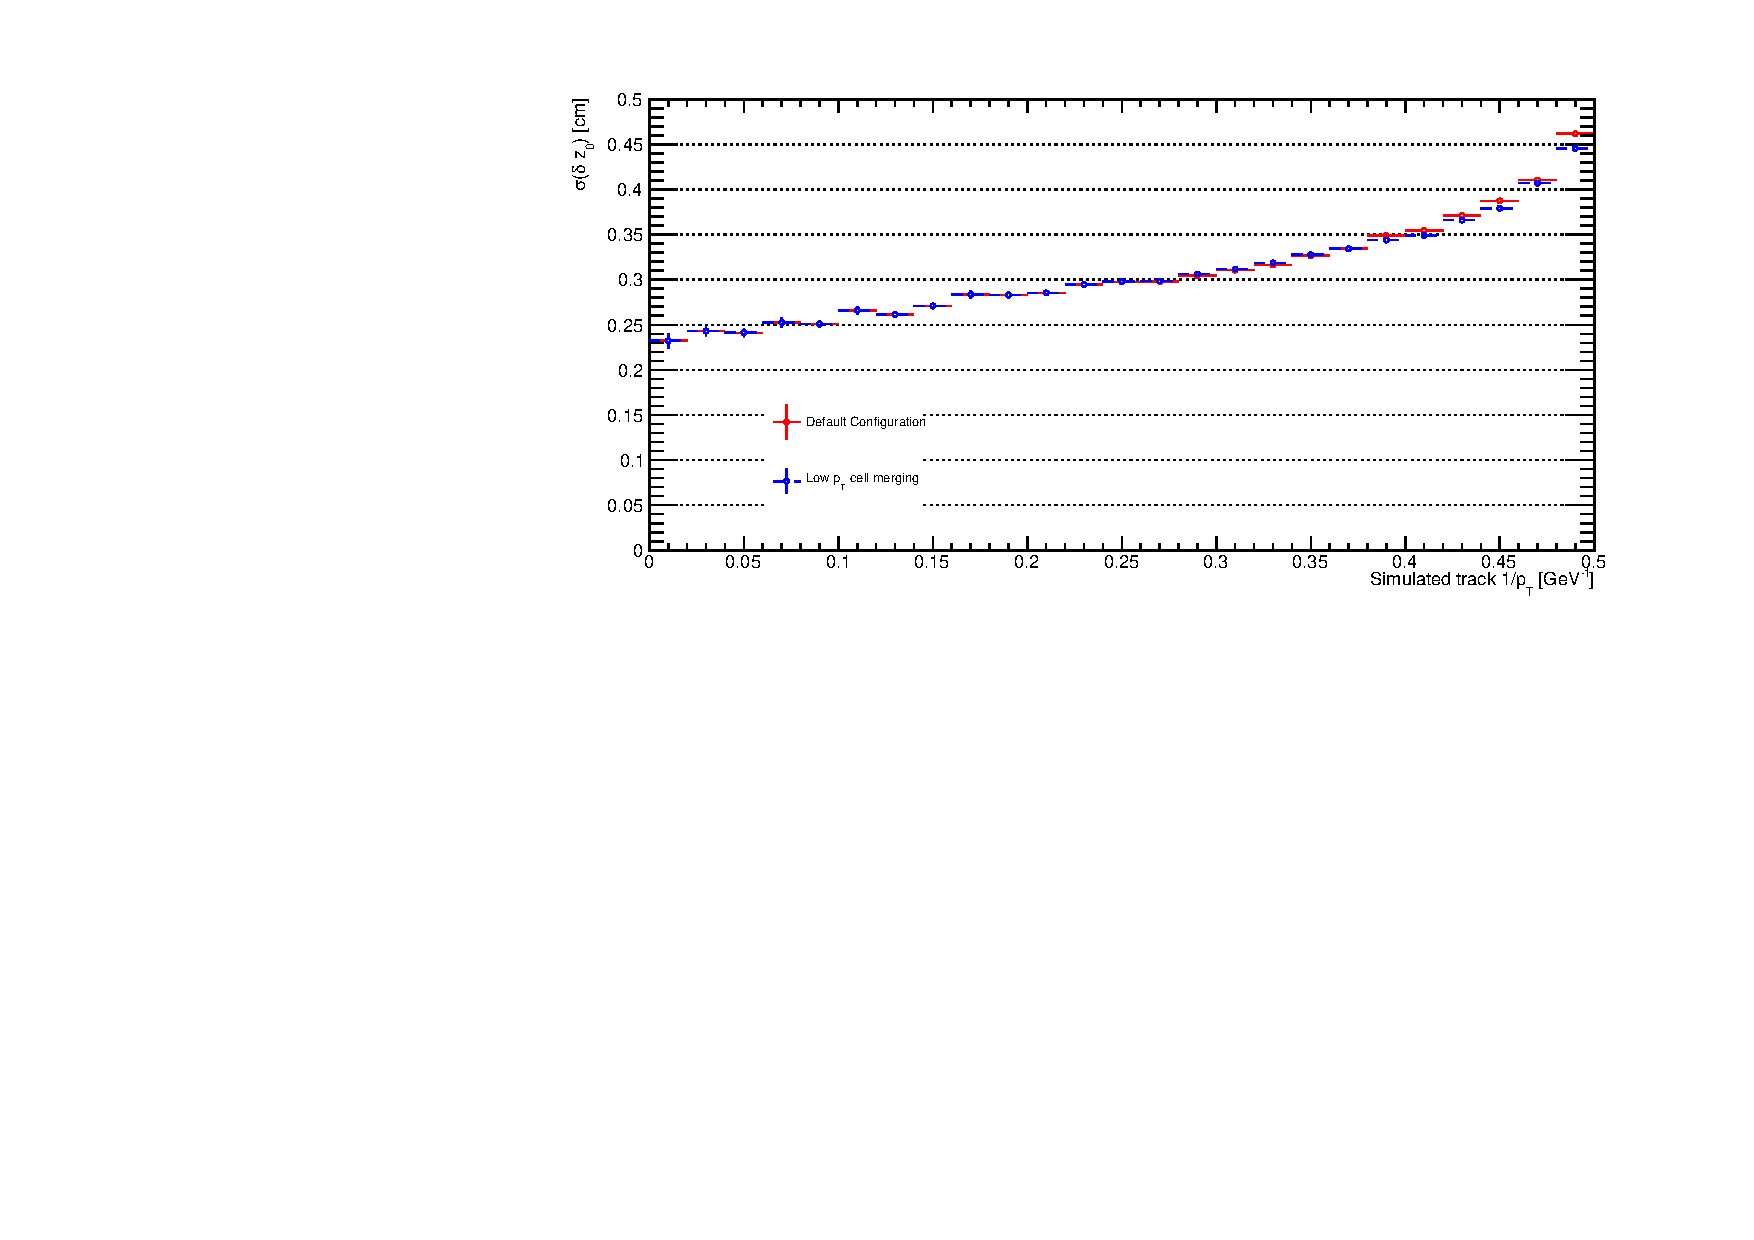
\includegraphics[width=0.49\textwidth]{figs/tk-upgrade/results-lowPtTracking/z0ResVsInvPtFlatGeometry_5000.pdf}
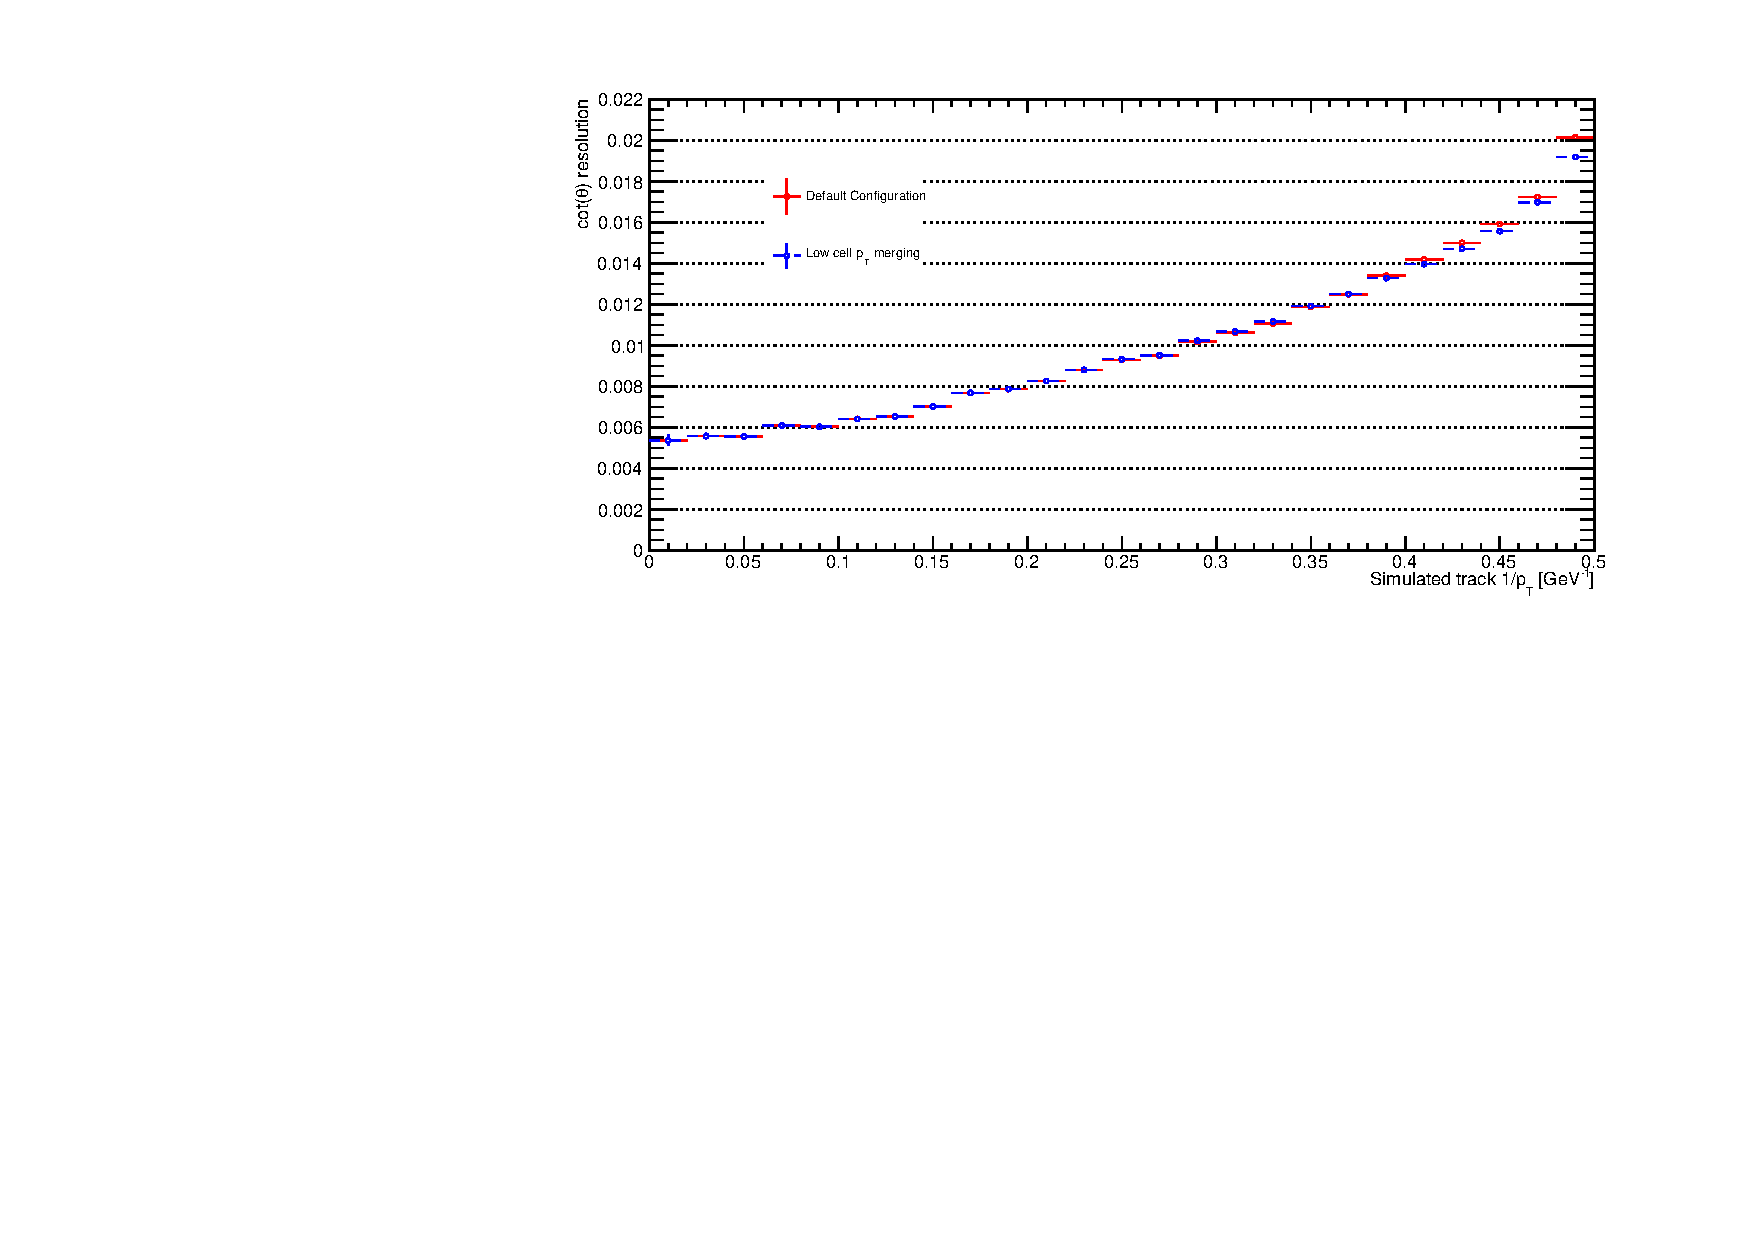
\includegraphics[width=0.49\textwidth]{figs/tk-upgrade/results-lowPtTracking/cotThetaResVsInvPtFlatGeometry_5000.pdf}
\caption{
The \pt resolution, $\phi$ resolution, $z_{0}$ resolution and cot$\theta$ resolution measured for both the default configuration where only the number of \HT \qpt columns have been increased (red) and after the \HT and \KF optimisations have been applied (blue) for primary reconstructed tracks in simulated \ttbar events at a <PU> of 200 for tracks with $\pt > 2\GeVc$.
\editComment{Make plots bigger!}
}
\label{fig:htHelixParametersResVsInvPt}
\end{figure}

\subsubsection{Kalman Filter Optimisation}\label{subsubsec:lowPtOptKF}
Incorporation of \MS into the \KF involved including a \emph{process noise} term, namely the variance of the multiple scattering angles, to the \emph{measurement noise} (\ie measurement error) term already present in the \KF covariance matrix.
In this updated form, the \KF now can consider stubs which are compatible with those that have undergone \MS, allowing tracks with previously discarded stubs to be reconstructed and the resultant more accurate $\chi^{2}$ values which can be used to better discriminate against fake track states.

For small deflection angles and relativistic particles, $\sigma_{\theta}$ for a each layer is given by~\cite{Lynch:1990sq}~:

\begin{equation}
\sigma_{\theta} = \frac{13.6\MeV}{\beta c p} q \sqrt{\frac{x}{X_{0}}} [1 + 0.088 \log_{10}{\frac{x}{X_{0}}}]  \;
\label{eq:scatter1}
\end{equation}

where, the momentum, velocity, electrical charge of the incident particle and thickness of the scattering medium in radiation lengths are given by $p$, $\beta c$, $q$ and $\frac{x}{X_{0}}$ respectively and the result being good to better than 11\%.

With the particles involved having relativistic velocities (\ie $\beta c \cong 1$) and scattering in the r-z plane ignored as the impact of multiple scattering is considerably smaller hit position resolution in r-z, the multiple scattering contribution in the \rphi plane can be expressed as:

\begin{equation}
\sigma_{\theta} = \frac{k}{\pT}
\label{eq:scatter2}
\end{equation}

where $k$ is a coefficient.

From the simplified form of Equation~(\ref{eq:scatter2}), two alternative forms of the coefficient $k$, which should require minimal resources and latency, were investigated:

\begin{itemize}
\item \textbf{constant coefficient - } a constant coefficient of the order of the average anticipated scattering angle is used as the anticipated typical scattering angle for $2-3\GeV$ tracks is of the order of a milliradian.
\item \textbf{layer dependent coefficient -} the coefficient used is a function of the layer ID (\ie which layer the stub is found) in order to take into account the impact of repeated scattering from passing through multiple layers increasing the uncertainty associated of the hit position.
\end{itemize}

The initial layer dependent coefficients were obtained through experimentally determining in simulation the \MS  contribution to the observed variance in $\phi$.
Both these initial layer dependent coefficients and the initial constant coefficient of a milliradian were subsequently further optimised in order to recover as much tracking efficiency as  possible.
Similarly, the \KF state $\chi^{2}$ cuts for both approaches were also tuned in order to reject the optimal number of fake and duplicate tracks without compromising on tracking efficiency.

During the comparative studies of these two approaches, as shown in figure~\ref{fig:2GeVfracDups} it was observed that following the \DR stage that the fraction of duplications present increases above circa $3\GeV$ in contrast to the trend of the fraction of duplicates decreasing as \pT decreases.
As this feature is present following the \HT stage, without any further stage being run, this implies that the \HT produces more duplicates at low \pT in the full precision cells.
As the fraction of duplicate tracks produced where decreased precision \HT cells are used is well controlled, the \pT threshold for the $2 \times 2$ merging of \HT cells was increased from $2.7\GeV$ to $3.5\GeV$.
While an increase in the duplicate rate is observed between $3.2\GeV$ and $5\GeV$ in figure~\ref{fig:2GeVfracDups}, a decreased number of duplicates were produced below $3.5\GeV$ which lead to an overall reduction in the number of duplicates produced of circa 2.8\%.

The increased \pT threshold for \HT cell merging also had the additional benefit of recovering an additional 0.2\% of the tracks which were previously lost to \MS.
Consequently, this change was adopted by the project and all the results presented below for the two \MS coefficient forms were produced using this increased threshold. 

\begin{figure}[tbp]
\centering
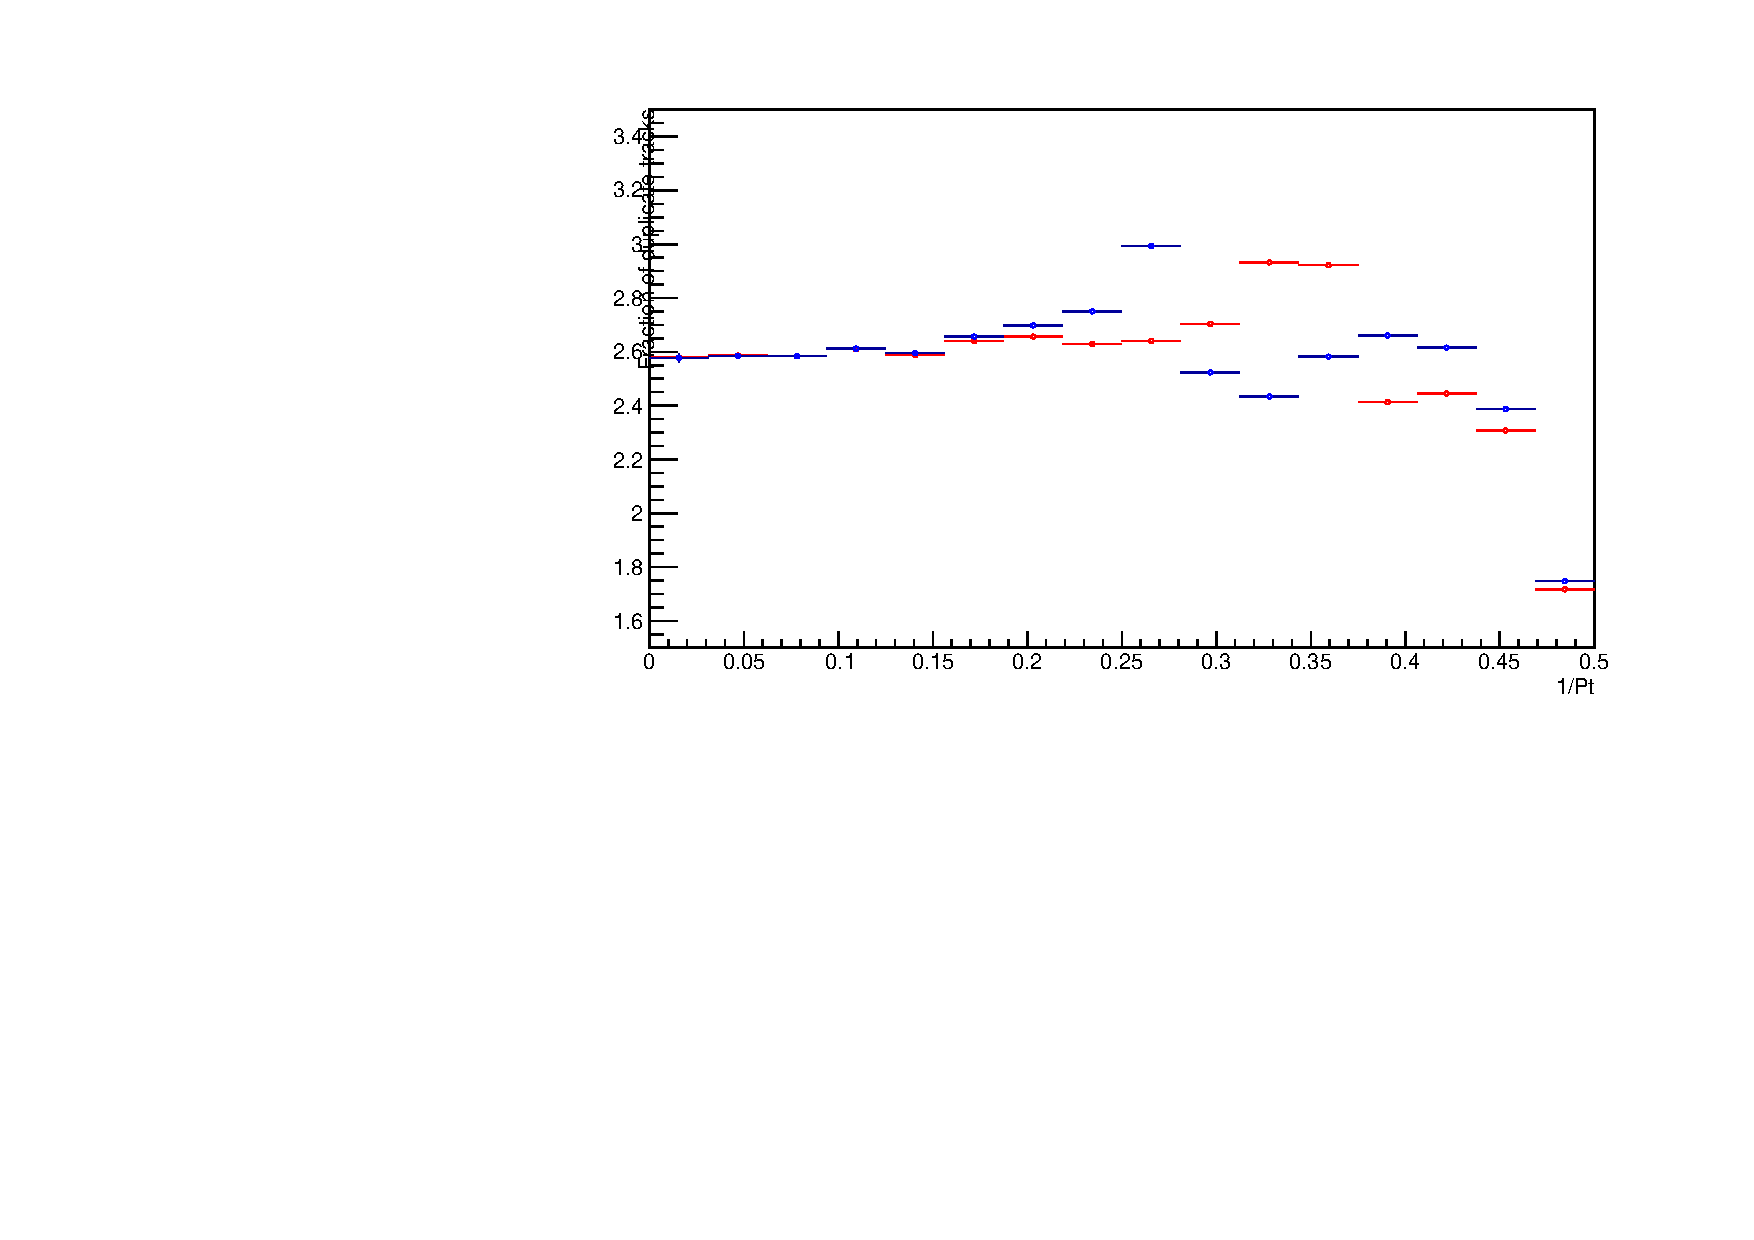
\includegraphics[width=0.49\textwidth]{figs/tk-upgrade/results-lowPtTracking/htFracDuplicatesVsInvPtTiltedGeometry_5000.pdf}
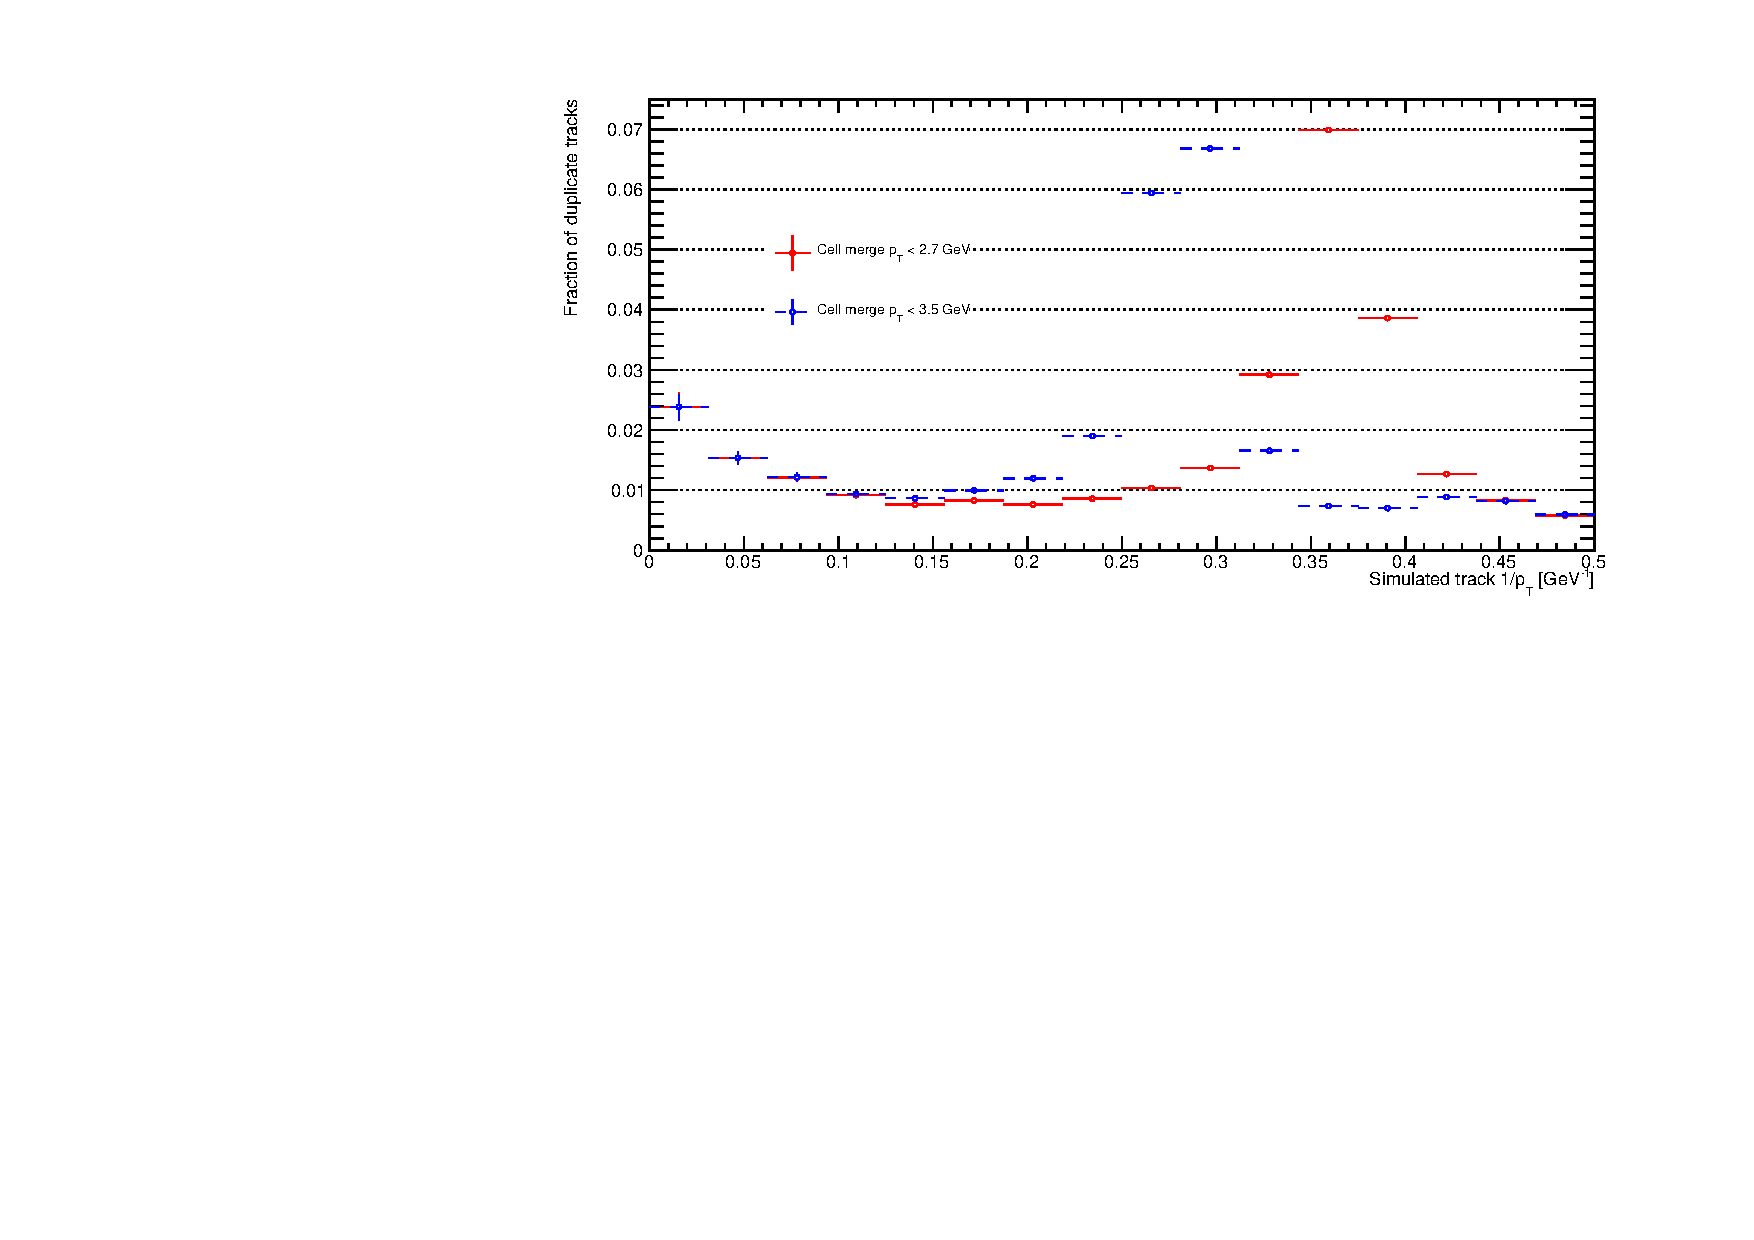
\includegraphics[width=0.49\textwidth]{figs/tk-upgrade/results-lowPtTracking/kfFracDuplicatesVsInvPtTiltedGeometry_5000.pdf}
\caption{The fraction of genuine tracks with duplicates as a function of $\frac{1}{\pT}$ following reconstruction by the \HT (left) and fitting and filtering by the \KF and \DR (right) for where the \HT cell merging \pT threshold is set to 2.7\GeV (red) and 3.5\GeV (blue). 
The constant coefficient for the \MS contribution was used for these \KF results.
\editComment{Resize plots!}
}
\label{fig:2GeVfracDups}
\end{figure}

\begin{figure}[tbp]
\centering
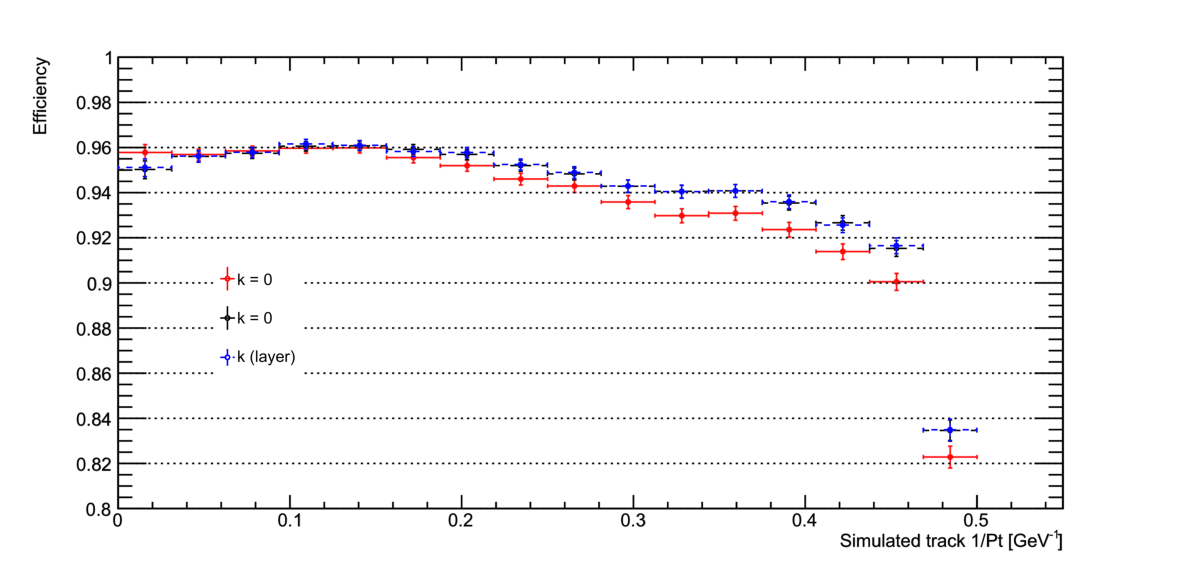
\includegraphics[width=\textwidth]{figs/tk-upgrade/results-lowPtTracking/kfTrackingEffVsInvPtTiltedGeometry_5000.pdf}
%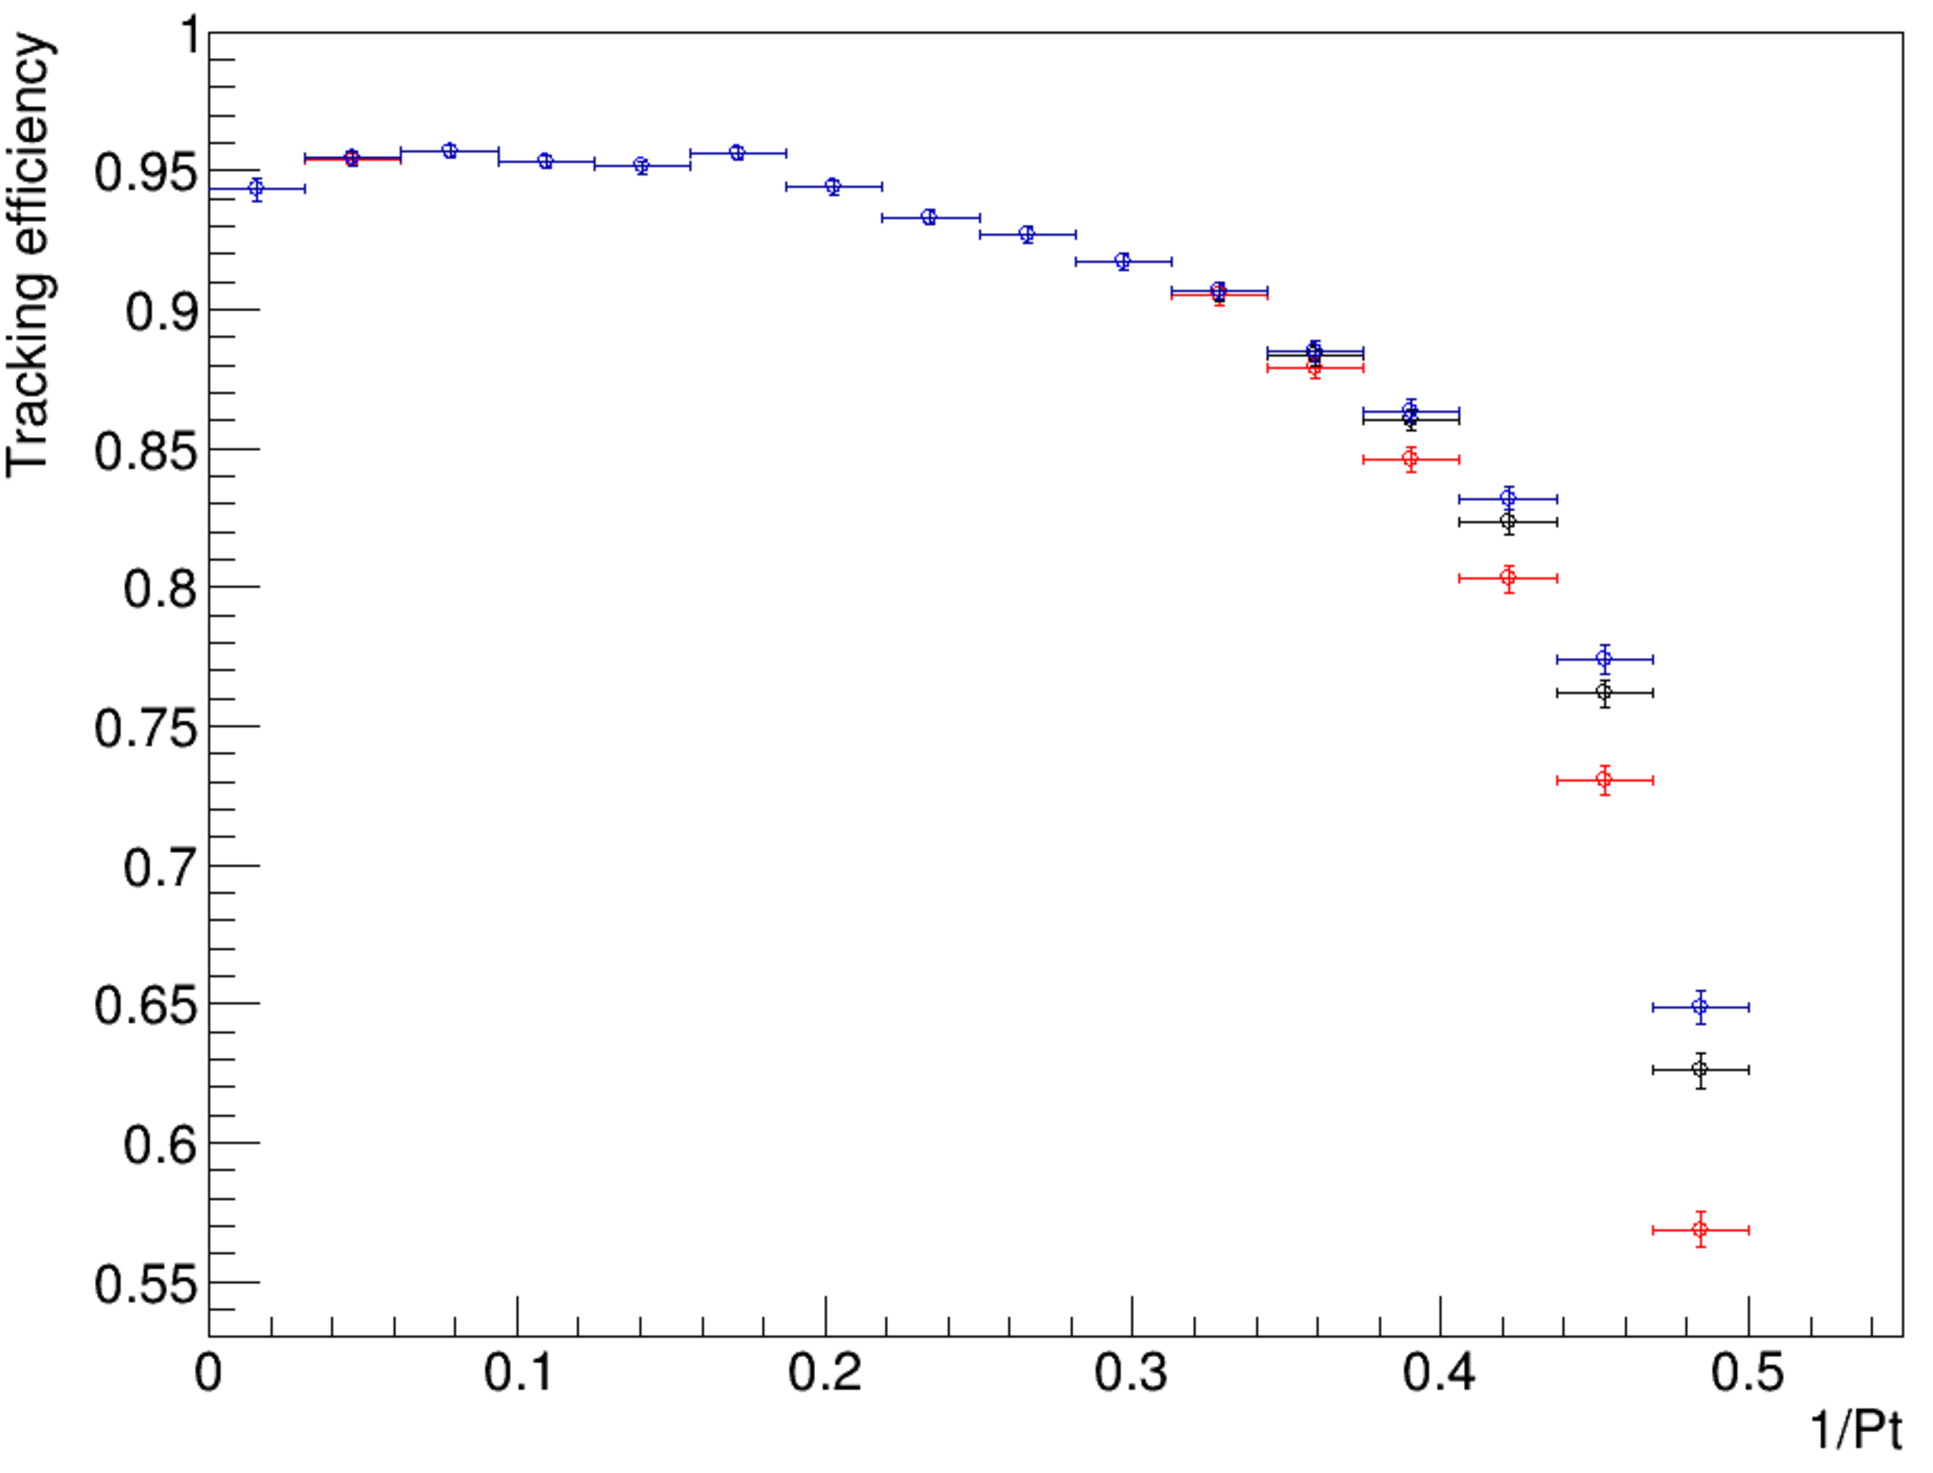
\includegraphics[width=\textwidth]{figs/tk-upgrade/results-lowPtTracking/kfTrackingEffVsInvPtFlatGeometry_5000.pdf}
\caption{Plots showing tracking efficiency as a function of $\frac{1}{\pT}$ for \ttbar events at a <PU> of 200 after the full chain has been run, where the \KF has not been modified to take \MS into account (red), a constant coefficient for \MS is used (black) and a layer dependent coefficient for \MS is used (blue).
}
\label{fig:2GeVTiltEff}	
\end{figure}

Figure~\ref{fig:2GeVTiltEff} shows how the tracking efficiency for the whole chain improves when \MS is accounted for in the \KF.
The similar performance observed between the two coefficients in figure~\ref{fig:2GeVTiltEff} and Table~\ref{tab:trackFindingPerformance2GeVKF} is due the amount of material traversed by a track not being constant for a single layer as the amount of material contributions in both the tracker and the prior contributions from the Inner Tracker, between the Inner and Outer Trackers and services varies as a function of $\eta$~\cite{P2TrackerTDR}.

Table~\ref{tab:trackFindingPerformance2GeVKF} also shows that compared to just the \HT optimisations alone, for both \MS coefficients, the \KF is more capable at rejecting incorrectly reconstructed tracks by up to an additional 3-4\%.
In contrast, the duplicate increases for both coefficients by 3-5\% for the full chain, with the increase in duplicates occurring between $3.2\GeV$ and $5\GeV$, as shown in figure~\ref{fig:2GeVfracDups}, near the $3.5\GeV$ threshold for merging adjacent \HT cells.
At the time of writing this chapter, it is not understood how incorporating \MS into the \KF causes this, but it is suspected to be related to the use of the reduced precision of \HT cells.
\editComment{It is hoped that by the time of submission, someone (Ian ... ?) will have figured this out.}
%Tracks with \pt approaching the \pt threshold at which reduced precision of \HT cells are used are have the potential to be built out of both stubs from both the full and reduced precision \HT cells.

\begin{table}[htbp]
\topcaption {Track finding performance on simulated \ttbar events at a <PU> of 200, after the full demonstrator chain for the three differing \KF configurations where \MS is not considered ($k = 0$), a constant \MS coefficient (const $k$) is used and a layer dependent \MS coefficient ($k(layer)$)is used. 
The track finding efficiencies following each stage are given using the efficiency definitions given in Section~\ref{subsec:helixParameter}, along with the mean number of tracks and the fraction of those tracks which are either fake or duplicate tracks.
\editComment{Fix table size!.}
}
\label{tab:trackFindingPerformance2GeVKF}
\centering
 \resizebox{\textwidth}{!}{
\begin{tabular}{ccccc}
   \hline
   \bf{Scattering coefficient} & \bf{Efficiency [\%]} & \bf{Mean \# of tracks} & \bf{Fakes [\%]} & \bf{Duplicates [\%]}  \\
   \hline
%     & \bf{HT}     &  96.2 & 752.0 & 28.2 & 47.3 \\  
   $k = 0$  & 93.6 & 216.0 & 13.3 & 9.4 \\      
   \hline
   const $k$ & 94.2 & 216.3 & 10.3 & 11.2 \\      
   \hline
    $k(layer)$ & 94.2 & 222.1 & 10.8 & 12.3 \\  
   \hline
   
\end{tabular}}
\end{table}

Figure~\ref{fig:kfHelixParametersResVsInvPt} shows the resolutions of the track parameters as a function of transverse momentum in simulation for tracks originating from the primary interaction in \ttbar events at a <PU> of 200 for both \MS coefficients considered as well as when \MS is not accounted for at all.
The resolutions of both \MS coefficients are superior across all \pt to when \MS is not considered at all, with the constant \MS coefficient typically providing more slightly more precise measurements than the layer dependent coefficient.  
As expected, lower transverse momentum tracks experience the greatest improvements given that \MS dominates at lower transverse momenta.
For both coefficients however, the \pt resolution in the range $ 3.8 \GeV < \pt < 5.5\GeVc$ is worse than when \MS is not considered.
At the time of writing, this observation is still being investigated, but is suspected, like the increased duplicate rate in the same \pT range, to be related to the reduced precision of \HT cells.

\begin{figure}[htb]
\centering
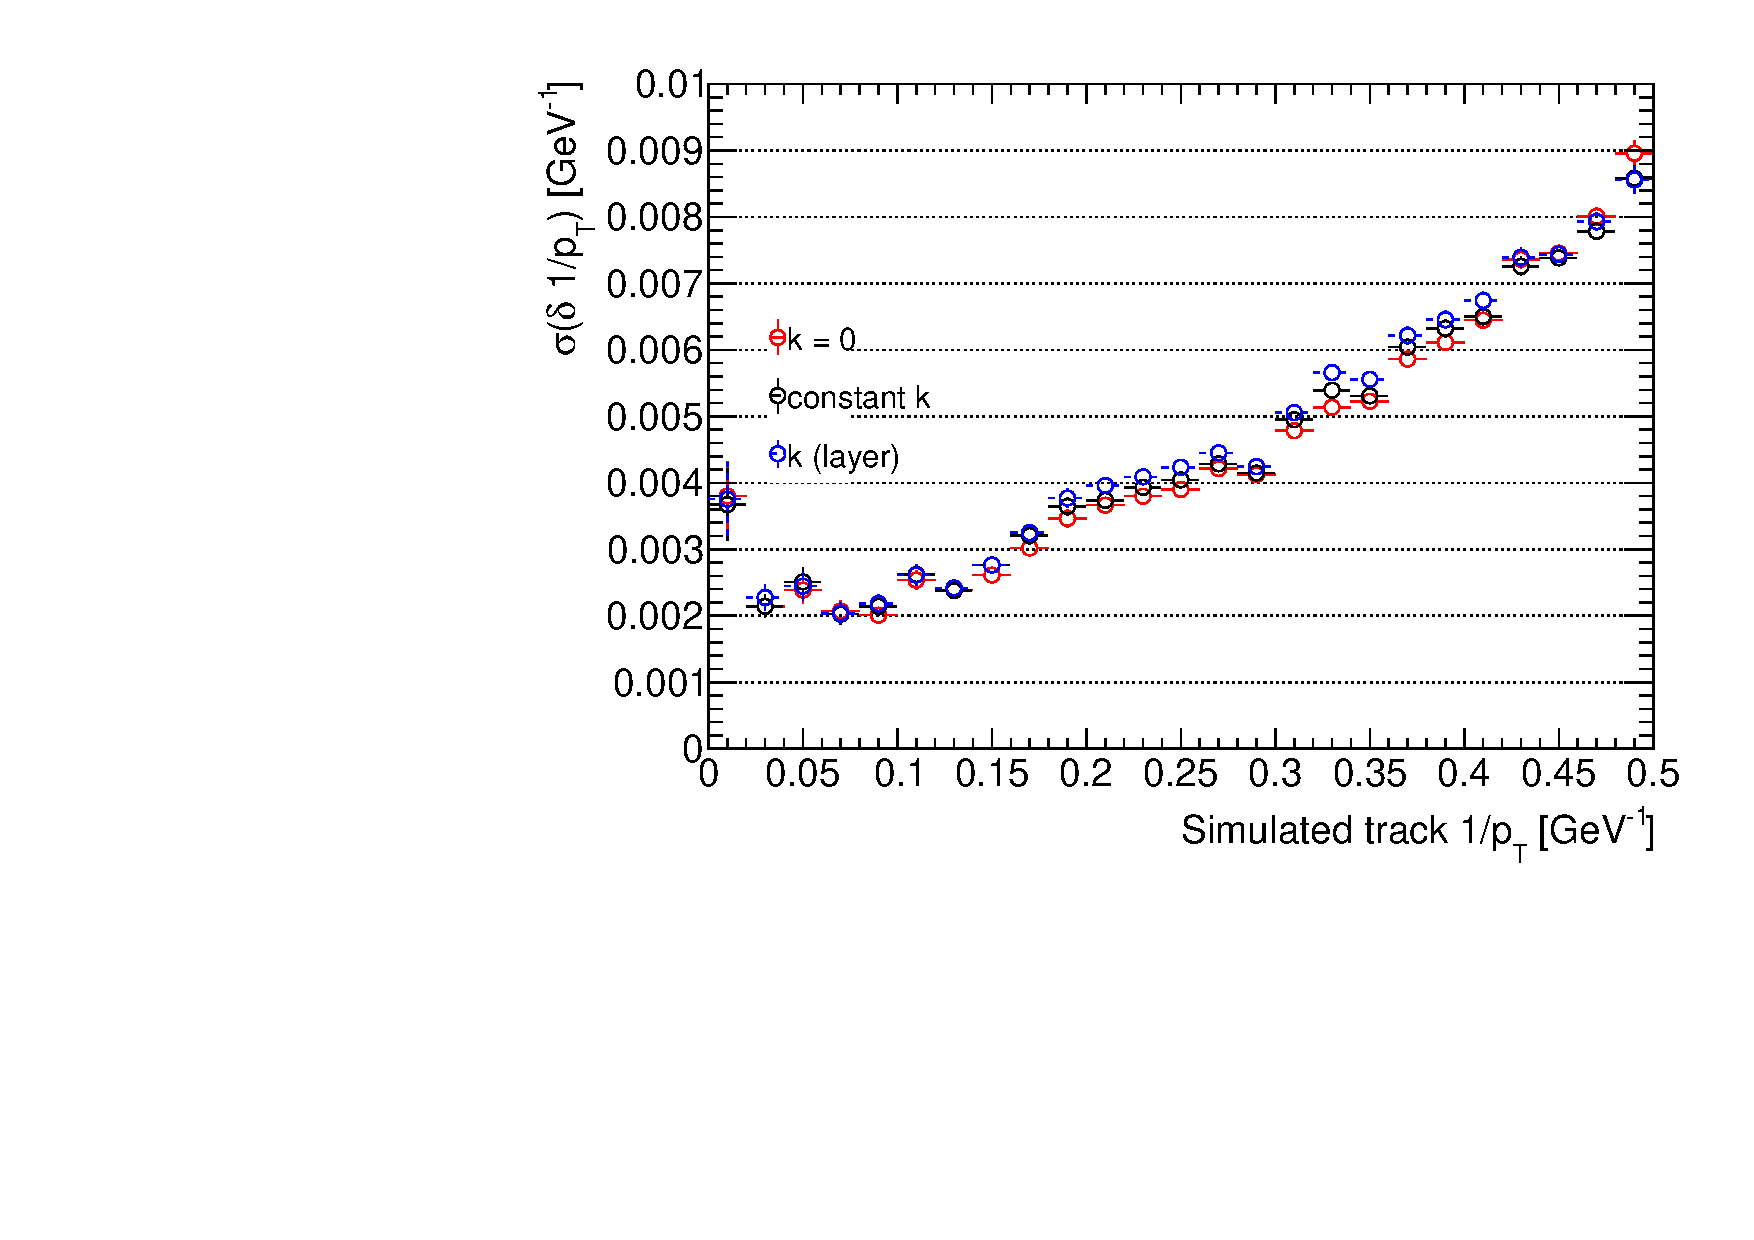
\includegraphics[width=0.49\textwidth]{figs/tk-upgrade/results-lowPtTracking/qOverPtResVsInvPtTiltedGeometry_5000.pdf}
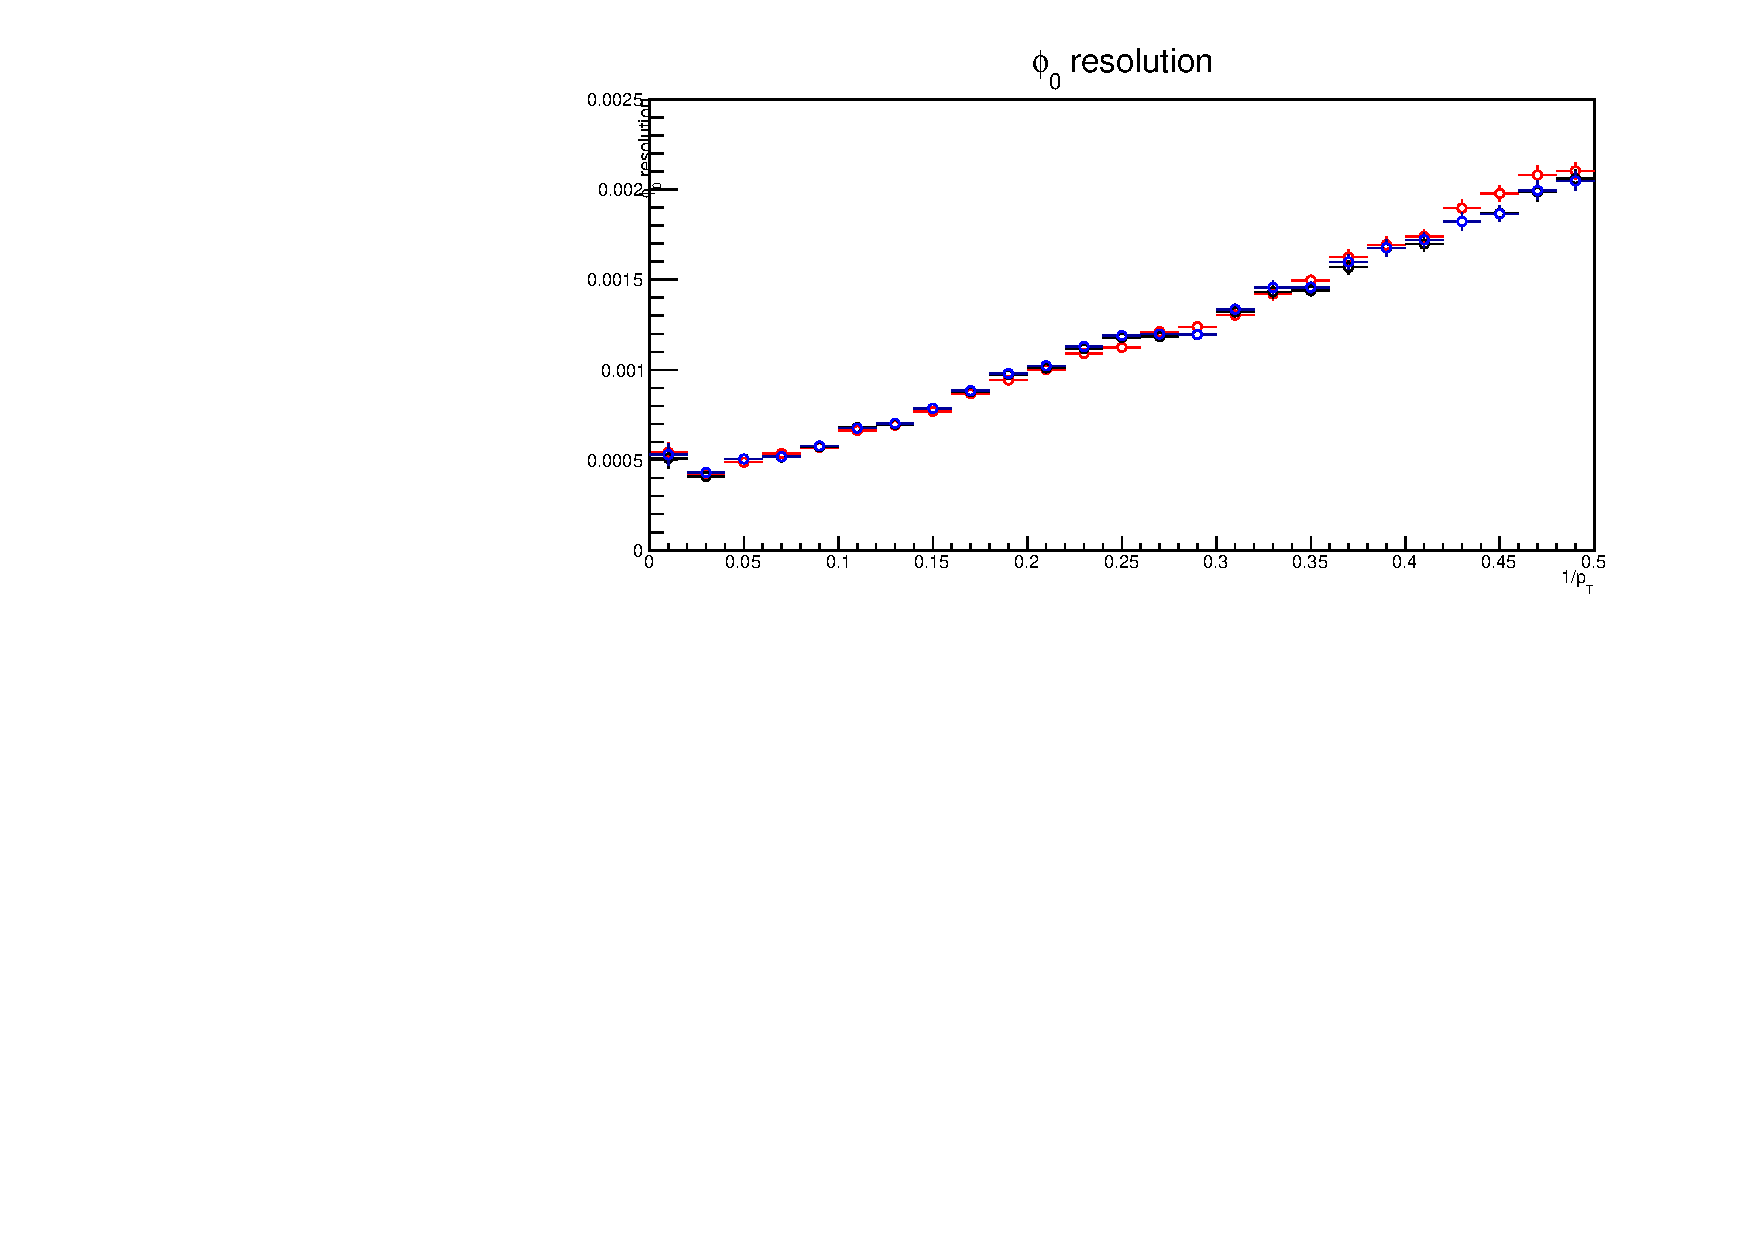
\includegraphics[width=0.49\textwidth]{figs/tk-upgrade/results-lowPtTracking/phi0ResVsInvPtTiltedGeometry_5000.pdf}
\\
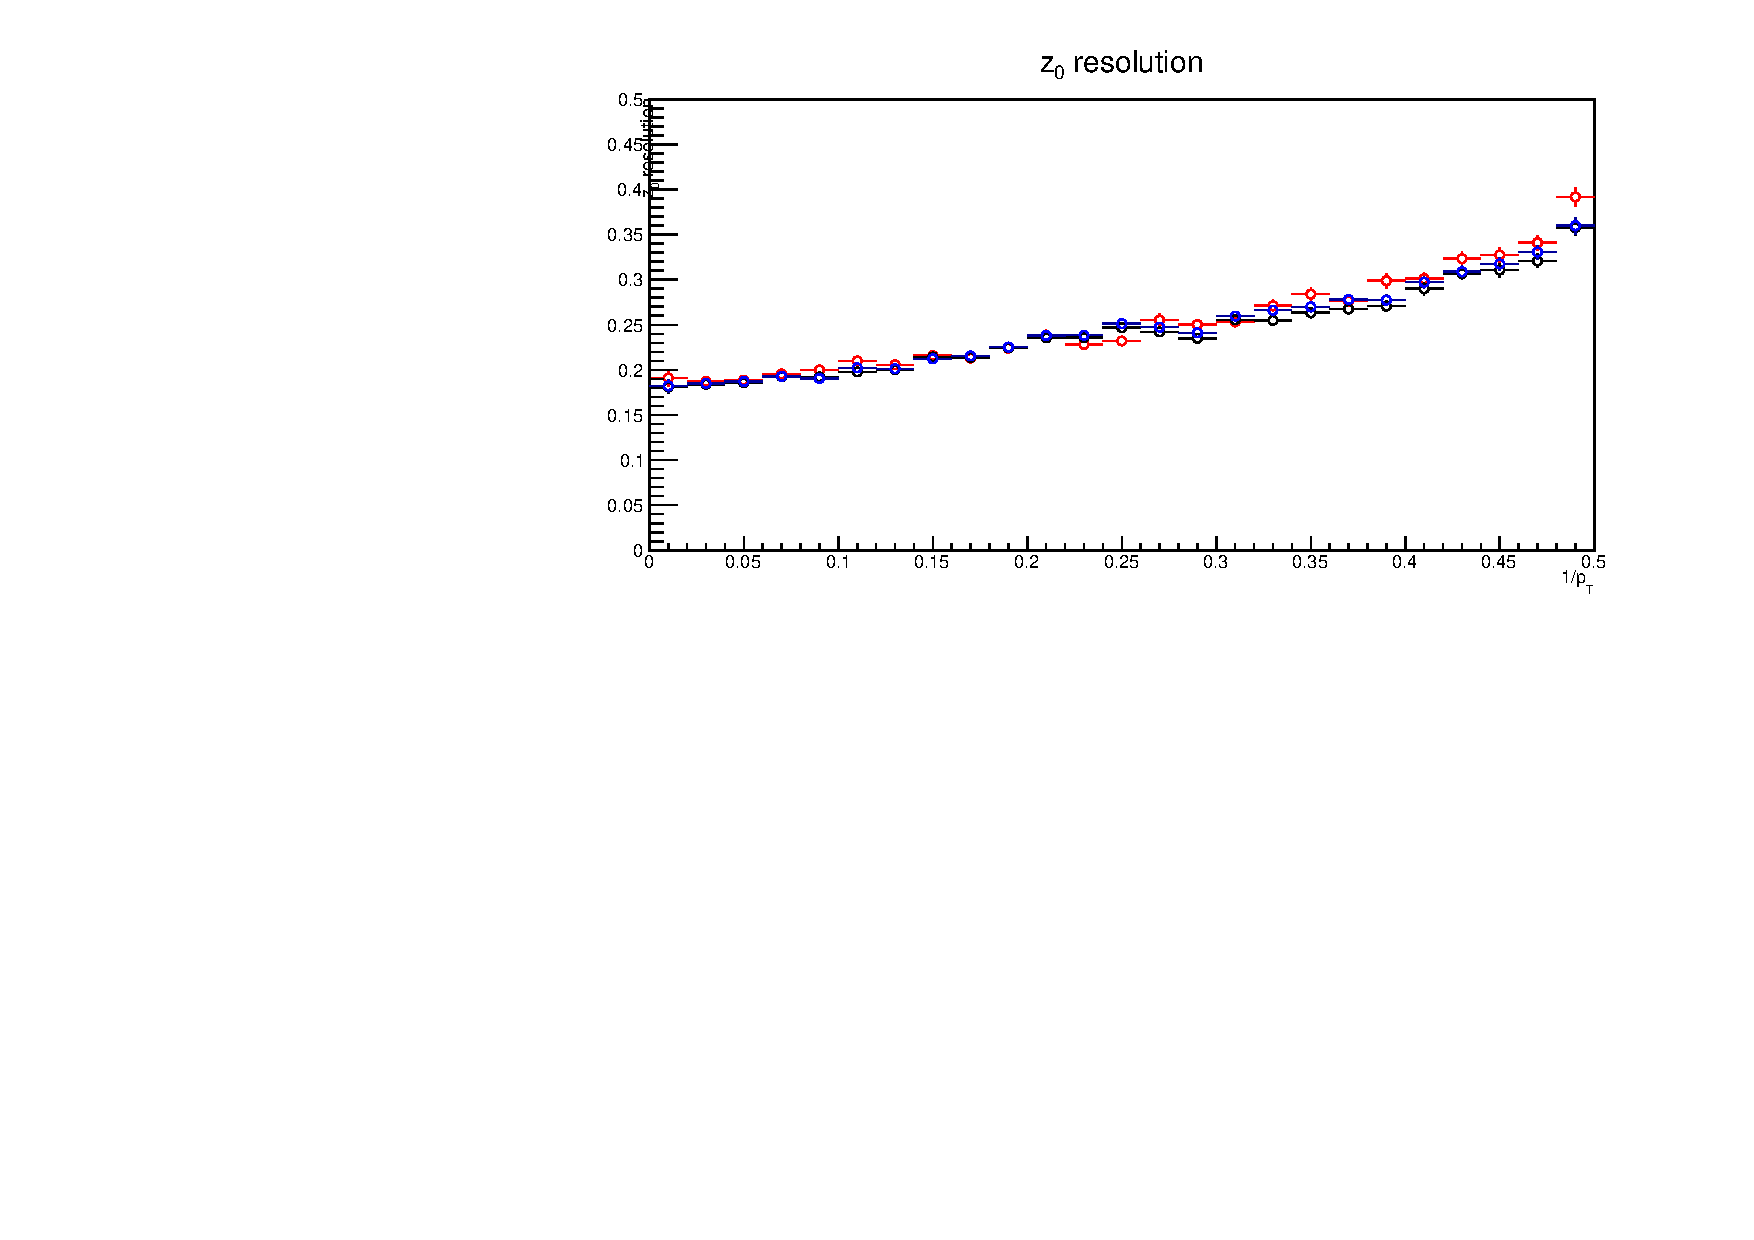
\includegraphics[width=0.49\textwidth]{figs/tk-upgrade/results-lowPtTracking/z0ResVsInvPtTiltedGeometry_5000.pdf}
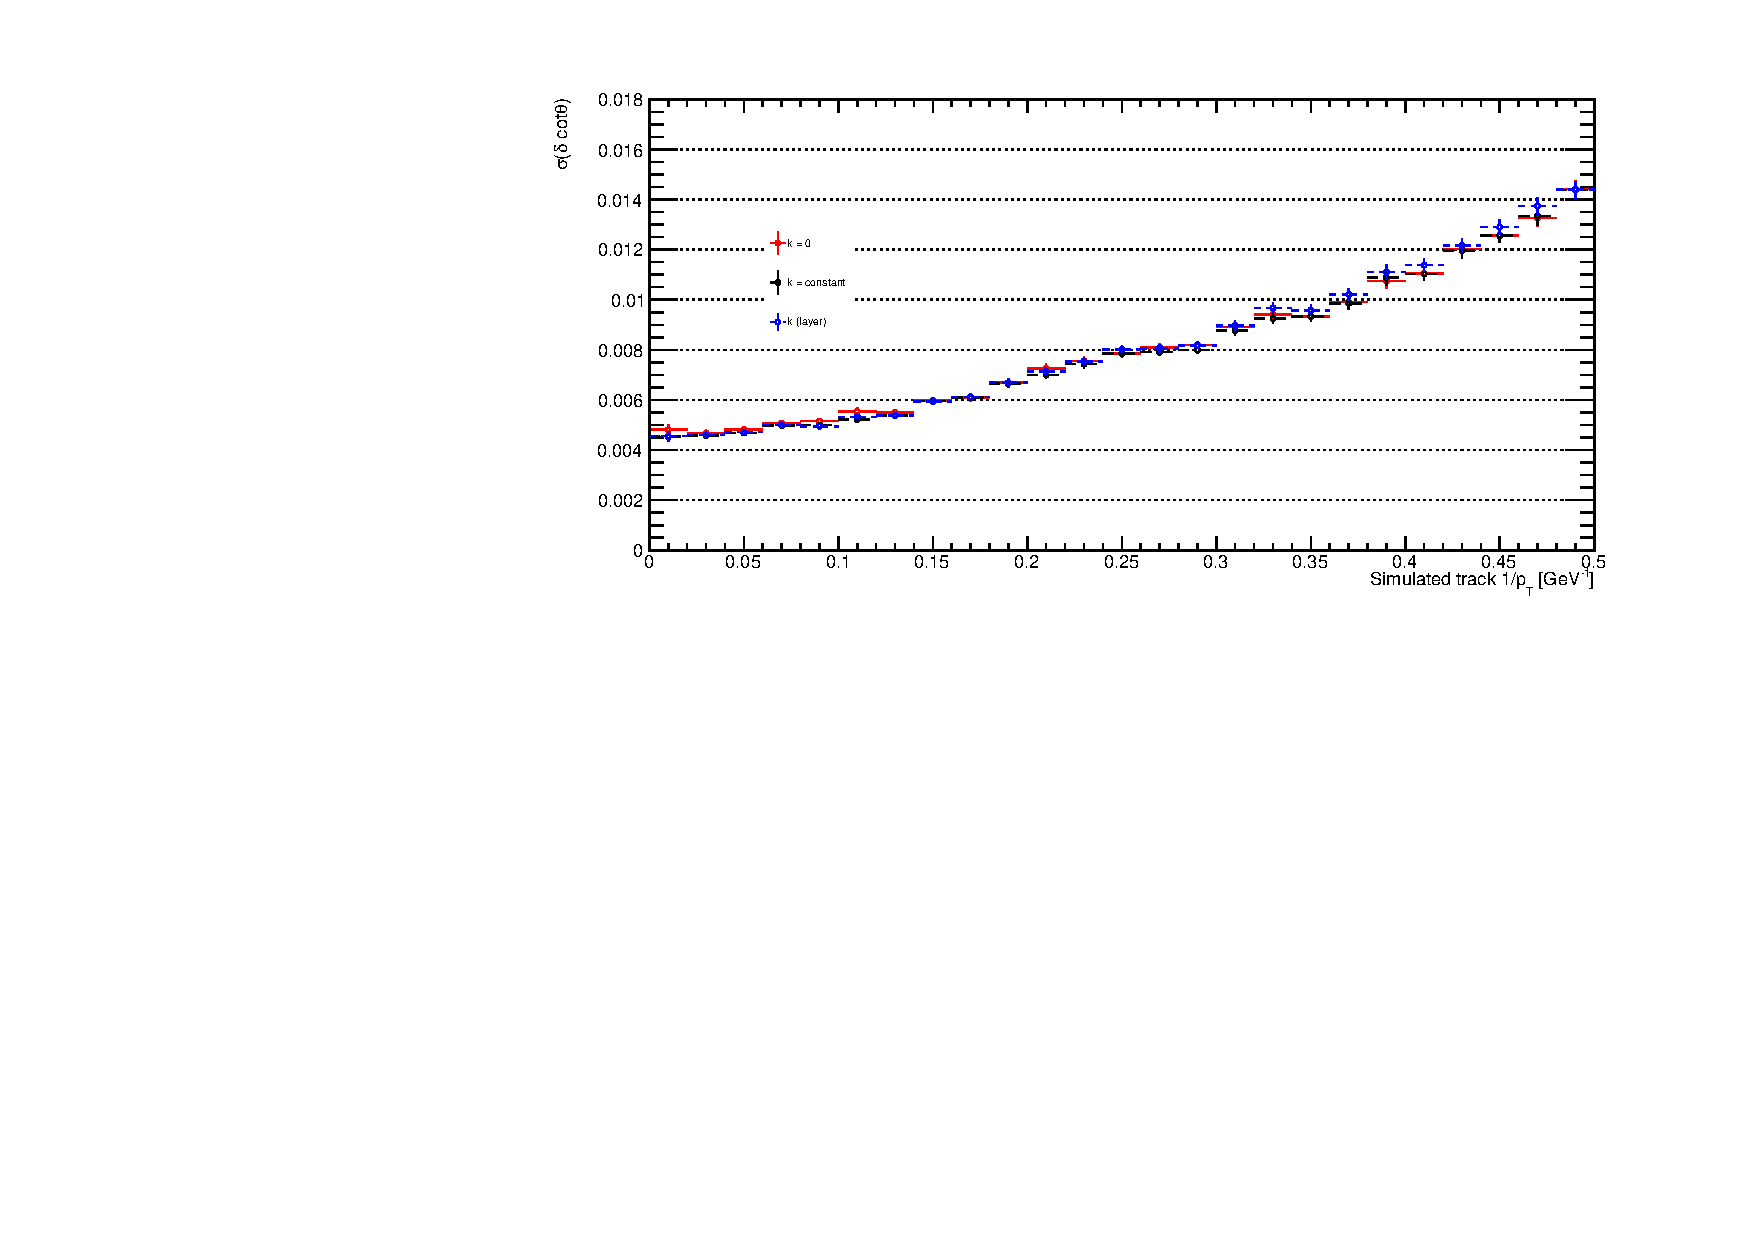
\includegraphics[width=0.49\textwidth]{figs/tk-upgrade/results-lowPtTracking/cotThetaResVsInvPtTiltedGeometry_5000.pdf}
\caption{\pt resolution, $\phi$ resolution, $z_{0}$ resolution and cot$\theta$ resolution measured for primary reconstructed tracks in simulated \ttbar events at a <PU> of 200 for when multiple scattering isn't considered by the \KF (red), when a constant \MS coefficient is used (black) and when a layer dependent coefficient is used (blue).
}
\label{fig:kfHelixParametersResVsInvPt}
\end{figure}

\subsubsection{Conclusions}\label{subsubsec:2GevConclusions}
After investigating modifications to the \HT and \KF algorithms to improve upon the default performance obtained for track finding and fitting of low \pT ($< 3\GeV$) tracks.
The decreased precision \HT cells enables the recovery of some of the tracks previously lost due to \MS, and the inclusion of a process noise term allows the \KF to take the impact of \MS into account, as shown in Figure~\ref{fig:2GeVTiltChi2Ndf} where the $\frac{\chi^{2}}{ndf}$ of the matched tracks fitted has not only decreased at high \pT where \MS dominates, but also the smaller effects experienced at higher \pT.
Both formulations of the \MS term provide considerable improvement in the track reconstruction efficiency and helix parameter resolutions obtained.
The lack of any noticeable improvement between using a constant \MS coefficient and one which is a function of the number of layers traversed, is a consequence of knowing which layer a hit belongs to not being a good descriptor of the total amount of material at that point.
As the amount of material traversed will depend on the trajectory of the charged particle, such a coefficient would likely have to be a function of \pt and $\eta$.

\begin{figure}[tbp]
\centering
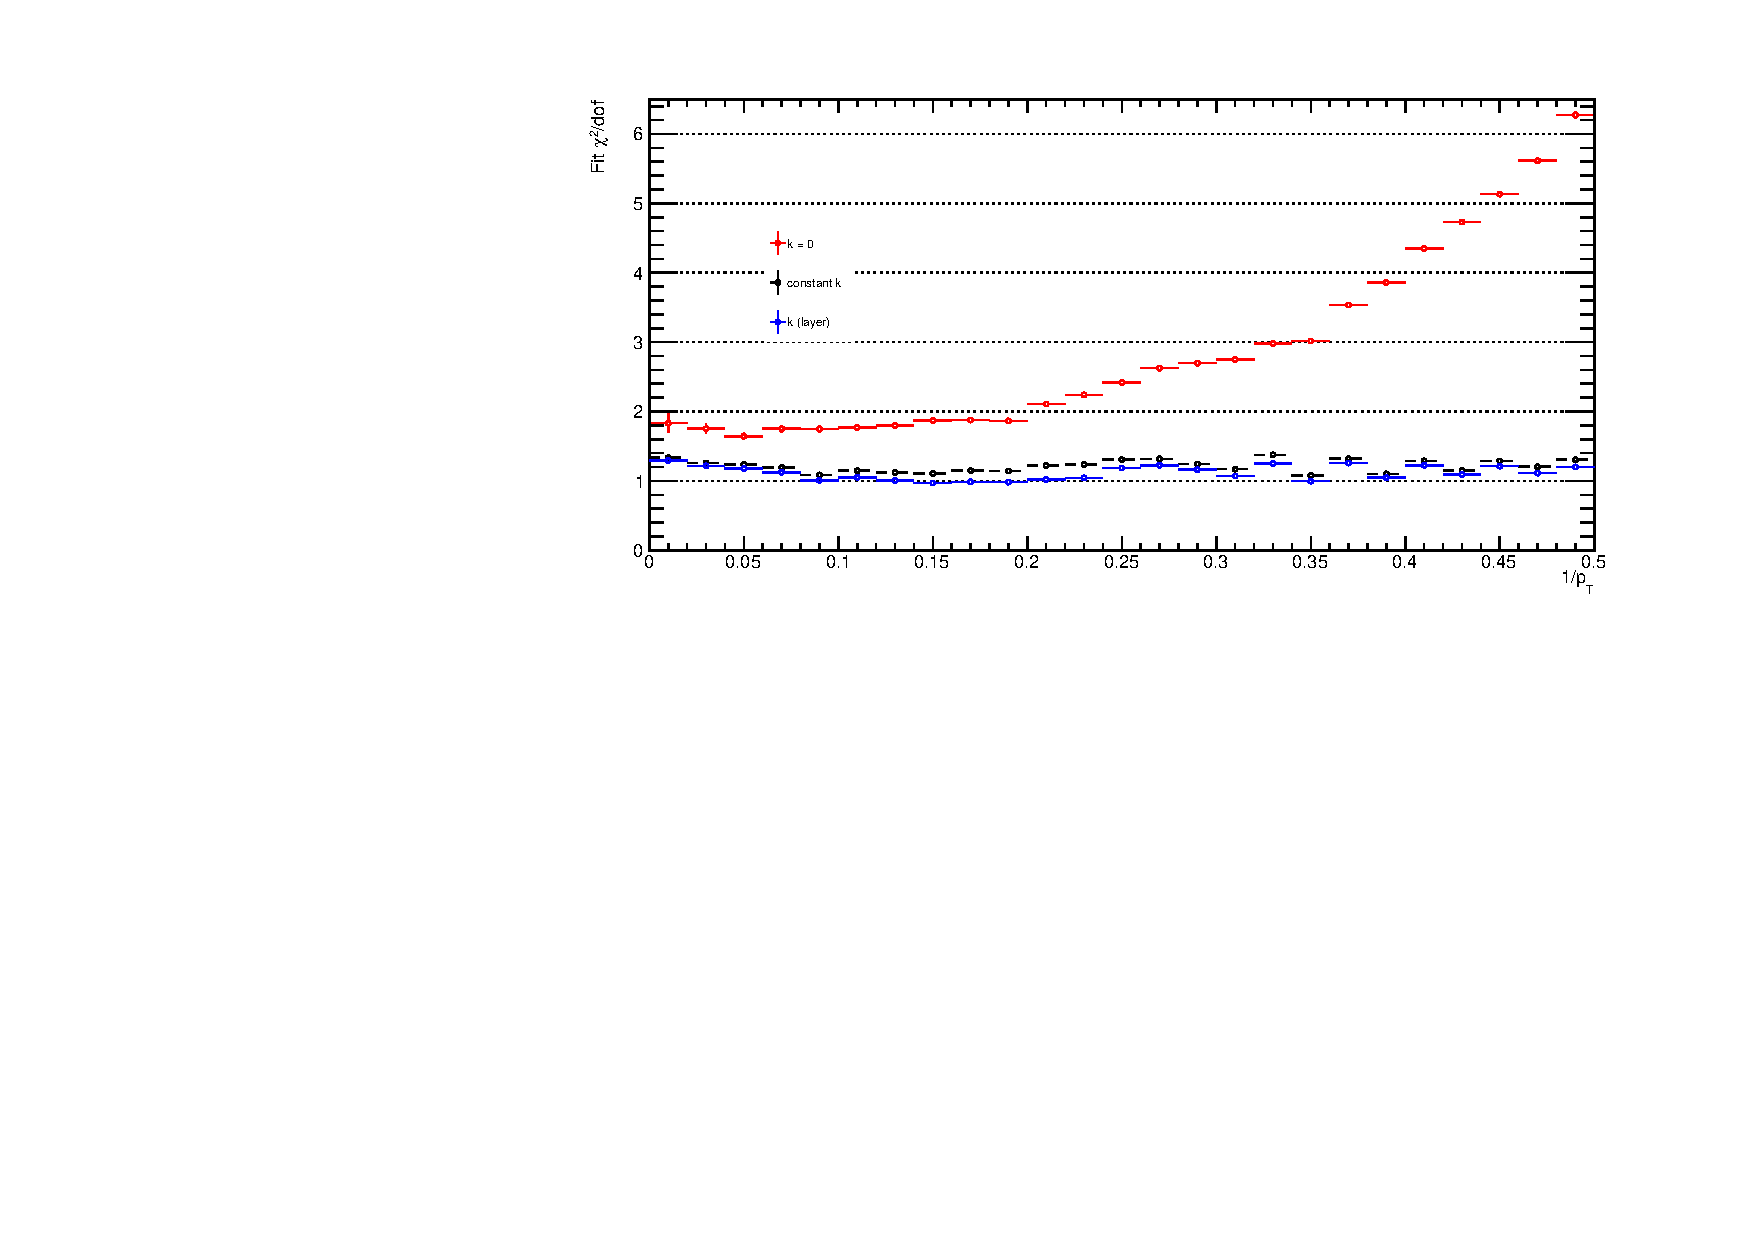
\includegraphics[width=\textwidth]{figs/tk-upgrade/results-lowPtTracking/kfChi2NdfVsInvPtTiltedGeometry_5000.pdf}
\caption{Plot showing $\frac{\chi^{2}}{ndf}$ as a function of $\frac{1}{\pT}$ for for \ttbar events at a <PU> of 200 after the full chain has been run, where the \KF has not been modified to take \MS into account (red), a constant coefficient for \MS is used (black) and a layer dependent coefficient for \MS is used (blue).
}
\label{fig:2GeVTiltChi2Ndf}	
\end{figure}


\chapter{Event Simluation and Object Reconstruction}\label{chapter:data-mc}
Following the readout of triggered events from the CMS detector, the reconstruction of the physics objects produced by the proton-proton collision is performed, allowing for the analysis of the underlying physical processes.
Monte Carlo (MC) simulations, which provide a detailed, precise and realistic description of the expected SM and potential BSM processes at the LHC, form an essential component of performing any analysis, allowing for the development of strategies to extract processes of interest from backgrounds and the ability to make statistical interpretations of the results, such as measuring and comparing the cross sections and other properties of a measured processes to theory or by setting limits on unobserved SM or predicted BSM processes.
The event simulation and objection reconstruction algorithms which are relevant to the single top physics search presented in this thesis are discussed in this chapter.

\section{Event Simulation}\label{sec:sim}
As MC simulation is meant to provide a realistic description of the expected SM and predicted BSM processes at the LHC, 
both accurate modelling of these processes and a detailed understanding of how physical processes interact with the CMS detector are required to produce events in the same format as raw proton-proton collision data prior to undergoing the same reconstruction process.
The simulation of events is a four stage process: generation (GEN), simulation (SIM), digitisation (DIGI) and reconstruction (RECO).

The initial GEN stage involves the use \emph{event generators} to simulate the proton-proton interactions and the resultant physics processes~\cite{Buckley:2011ms,Hoche:2014rga}.
The first stage of this is the modelling of the colliding protons and the hard scattering of their constituent partons, which involves the use Parton Distribution Functions (PDFs) to assign fractions of the proton's momentum to the partons and perturbation theory to compute the Matrix Elements (ME) of the Feynman diagrams for the QCD and electroweak processes involved.
The second stage models resultant Parton Showers (PS) through an iterative process until the infrared cutoff scale for the shower is reached, with the remaining particles undergoing hadronisation.
The various event generators used in the production of MC samples used in this thesis are discussed in~\ref{subsec:eventGenerators}.

Following the GEN stage, the SIM stage involves passing the GEN output through a complete simulation of the CMS detector that has been with the GEANT4 program~\cite{geant4,Lefebure:1999wja}.
This process models particle interactions and decays and the propagation of particles through the detector, the effects of solenoidal field and detector material.
The DIGI stage uses the SIM output to produce the detector's electronics response, which then undergoes the same RECO process that data does, as described in~\ref{sec:reco}.

The inelastic proton-proton interactions, typically called pileup (\PU), which occur both within and adjacent to the event's bunch crossing, referred to as \emph{in-time} and \emph{out-of-time} \PU  respectively, also require modelling in simulation.
Simulated \PU however, does not adequately describe observed \PU in data.
Therefore, the reweighting of the simulated samples is required and is discussed in~\ref{}.

\subsection{Event Generators}\label{subsec:eventGenerators}
A number of event generators are used by CMS to produce the MC simulation samples used to describe the expected processes produced at the LHC.
Whilst there are several general-purpose event generators which can describe an event from the initial hadron collision to final state particles, they are typically used in conjunction with generators that specialise in a specific physics aspect (\ie ME calculations or PS simulation) or process (\eg tau decays) in order to provide a complete event.
Perturbative calculations of the MEs of the QCD and electroweak processes are done, where possible, to Next-To-Leading Order (NLO) in order to both enable precision measurements to be made and to accurately model processes with many distinct high energy jets.

The MC samples used to model the background and signal processes for the analysis presented in this thesis were simulated using the following generators:

\begin{itemize}
\item \textbf{Madgraph} - Madgraph~\cite{Alwall:2011uj} is a package which performs tree-level perturbative calculations to produce matrix elements at Leading Order (LO) for processes such as decays and 2 \rightarrow n scatterings through evaluating the ME for a given phase space point for all the Feynman diagrams produced.
\item \textbf{aMC@NLO} - aMC@NLO~\cite{Alwall:2014hca} is a package that considers tree-level and one-loop Feynman diagrams to produce matrix elements at NLO.
Considering the constructive and destructive interferences which result from considering both the leading and higher order cross section terms results in positively and negatively weighted events.
These negatively weighted events cannot be simply discarded as they are required to correctly simulate the NLO cross section.
The treatment of these negative weights in the analysis presented is discussed in Chapter~\ref{}.
\item \textbf{POWHEG} - The Positive Weight Hardest Emission Generator (POWHEG)~\cite{Alioli:2010xd} is a framework that interfaces NLO ME calculations with PS generators.
As its name suggests, POWHEG produces the hardest emission first through using the exact NLO ME and produces only positively weighted events.
The latter is achieved by interfacing to a PS generator which order emissions by \pT or allows for the use of a $p_{T}$-veto to reject subsequent emissions, avoiding double counting such emissions and the need for negative weights.
\editComment{Worth mentioning angular ordered generators? Wary of needing to defend that several levels beyond what is written.}
\item \textbf{PYTHIA} - PYTHIA~\cite{Sjostrand:2014zea} is a general-purpose generator which is used to take the output of the above ME event generators and perform the parton showering and hadronisation to produce the full event.
\end{itemize}

\section{Object Reconstruction}\label{sec:reco}
Using the readouts of all of the CMS sub-detectors, a full reconstruction of the triggered physics event is undertaken.
This process involves the \emph{Particle Flow} (PF) algorithm which combines the complementary information from each of the CMS sub-detectors, known as \emph{elements}, to provide an optimal reconstruction and identification of all of the stable particles present in the event~\cite{CMS:2009nxa,CMS:2010eua,CMS-PRF-14-001}.
Using these reconstructed particles, additional objects such as b-jets and missing transverse energy can also be constructed.

\subsection{Charged Particle Tracks}\label{subsec:tracks}
As the charged particles produced from the proton-proton collisions traverse the silicon tracker, they interact with it and leave energy deposits known as \emph{hits}.
These hits are used to reconstruct the particles' trajectories through multiple iterations of the Combinatorial Track Finder (CTF) algorithm, which is based off combinatorial Kalman Filtering~\cite{Chatrchyan:2014fea,Fruhwirth:1987fm}.

The steps of each iteration	of the CTF algorithm are:
\begin{itemize}
\item \textbf{Seed generation:} initial track candidates are formed from two or three hits to provide a first estimate of the tracks' helix parameters.
\item \textbf{Track Finding:} A combinatorial Kalman Filter then builds a candidate by adding hits from successive layers which are compatible with the extrapolated trajectory, which is updated with the addition of each subsequent hit, taking into account the hit's position, uncertainty and material traversed.
\item \textbf{Track Fitting:} The initial estimate of a built track's parameters is improved upon with the Kalman Filter performing two passes, the first from the innermost layer outwards and the second from the outermost inwards.
This approach minimises the bias in determining and discarding which hits are incorrectly associated with the track.
\item \textbf{Track Selection:} Quality criteria, such as $\chi^{2}$, the number of layers with hits and compatibility, are used to reject \emph{fake} tracks which are not associated with a charged particle.
\end{itemize}

Up to six iterations of the CTF are performed, with selected tracks' hits removed from consideration by subsequent iterations.
Whilst initial four iterations use seeds exclusively from the pixel tracker, the last two iterations use seeds from the strip tracker to enable a high track reconstruction efficiency for those originating outside the pixel or those which did not leave any hits in the pixel tracker.

\subsection{Primary Vertices}\label{subsec:vertices}
The reconstructed tracks are subsequently used to reconstruct the positions where the proton-proton collisions occurred, known as the \emph{primary vertices}~\cite{Speer:2006mh,Chatrchyan:2014fea}.
Initially tracks are required to be consistent with originating promptly from the interaction region, namely having a small transverse impact parameter, a minimum number of hits in the pixel and strip trackers and a low normalised $\chi^{2}$.
Such tracks are then clustered along the z-axis at their point of closest approach to the beamspot using a deterministic annealing algorithm	~\cite{Kenneth:1998i}, with these vertex candidates being used as input to an adaptive vertex filter~\cite{Fruhwirth:2007hz} to provide 3D position fits, uncertainties and variables such as the number of degrees of freedom to discriminate against fake vertices.
Out of these resultant primary vertex candidates, the one with the greatest scalar transverse momentum is considered as the \emph{primary vertex}, with the rest being considered \PU vertices.
Displaced vertices, such as those from heavy hadrons, are reconstructed during later reconstruction stages.

\subsection{Calorimeter Energy Clusters}\label{subsec:clustering}
The energy deposited by particles in the calorimeters is independently clustered in each sub-detector, except for the HF where each large cell can give rise to one cluster, to determine the energy and direction of the particles~\cite{CMS:2009nxa}.

The clustering algorithm consists of three steps:
\begin{itemize}
\item \textbf{Cluster seeding} - local cells' energies above a thresholds are considered as seeds.
\item \textbf{Clustering} - adjacent cells are summed together to form topological clusters.
\item \textbf{Energy threshold} - if the energy of the cluster is greater than two standard deviations of the electronics noise (80\MeV in the EB, up to 300\MeV in the EE, and 800\MeV in the HCAL), the cluster is accepted.
\end{itemize}

\subsection{Particle Flow Algorithm}\label{subsec:PF}
Through combining the calorimeters' energy clusters and charged particle tracks from the tracker and muon systems, the Particle Flow algorithm is able to use all the available information from an event to reconstruct and identify all stable particles in an event with far superior results than if each sub-detector were used individually.

The initial stage of the process involves associating charged particle tracks to energy clusters from the ECAL and HCAL sub-detectors.
Tracks are extrapolated from the last hit in the tracker to the typical shower profiles in the calorimeters, and if the particles' expected positions in the calorimeters are within the clusters' boundaries, these elements are linked together.

These linked elements are used by the Particle Flow algorithm to sequentially reconstruct and identify PF particles, removing classified elements from further consideration, with the least ambiguous or cleanest objects reconstructed first, followed by progressively more difficult objects which can be constrained by previous ones.

This is done in the following order: 
\begin{itemize}
\item muons are reconstructed, as described in Section~\ref{subsec:muons}.
\item electrons and associated Bremsstrahlung photons and isolated photons are reconstructed, as described in Section~\ref{subsec:electrons}.
\item charged hadrons are reconstructed from the HCAL clusters which are compatible with the remaining ECAL clusters and charged particle tracks.
\item any remaining ECAL and HCAL clusters with no associated charged particle tracks are reconstructed as photons and neutral hadrons respectively.
\item a post-processing stage is undertaken to mitigate against the small probability of misidentified or reconstructed particles, usually high momentum muons, causing the appearance of a large amount of missing transverse energy being present.
\end{itemize}

\subsection{Electrons}\label{subsec:electrons}
Electrons lose on average between 33\% (minimal intervening material) and 86\% (maximum intervening material) before reaching the ECAL due to producing Bremsstrahlung photons in the tracker layers~\cite{Khachatryan:2015hwa}, which often undergo electron pair production, producing further Bremsstrahlung photons.	
It is essential that this radiated energy is collected in order to correctly determine an electron's initial energy.
ECAL clusters, known as \emph{superclusters} (SCs), have an extended window in $\phi$ as the magnetic field bends electrons trajectories in the $\phi$ direction whilst photons are unaffected, causing an energy spread across $phi$.
Two clustering algorithms are used to form SCs of $5 \times 1$ and $5 \times 5$ arrays of ECAL crystals in the EB and EE respectively due to their different geometrical arrangements.
Both of these ECAL clustering algorithms are discussed in greater detail in~\cite{Khachatryan:2015hwa}.
The presence of Bremsstrahlung also necessitates the use of a Gaussian Sum Filter (GSF)~\cite{Adam:2003eca} to fit electron tracks instead of a Kalman Filter as the process is non-Gaussian and Kalman Filters only assume Gaussian noise contributions.
The computationally heavy nature of the GSF algorithm however, limits its use to refitting \KF track seeds which have a significant presence of Bremsstrahlung and for the final fitting of a track's parameters.

%%% Track seeding
Electron track seeds formed of the initial two or three hits in the tracker from which tracks are built from are constructed by two complimentary algorithms~\cite{Khachatryan:2015hwa}:
\begin{itemize}
\item \textbf{ECAL-based approach} - an electron's SC's energy and position is used to extrapolate the expected electron trajectory towards the primary vertex in order to determine where hits are anticipated to be for both electrons and positrons.
Reconstructing electrons in jets however, suffers from large inefficiencies due to the potential to incorrectly associate hits from other charged particles with the track and the jet energy deposits  overlapping with the electron SCs impacting the assumed energy and position of the SC.
Low \pT electrons are also poorly described as the increased bending of their trajectories results in the spread energy not being fully contained by a SC.
\item \textbf{tracker-based approach} - this approach is designed to compliment the ECAL-based approach by being able to reconstruct non-isolated and low \pT electrons efficiently.
A \KF is initially used for track finding which is able to accurately reconstruct electrons that emit limited Bremsstrahlung in the tracker, with the KF track matched to the closest ECAL SC.
Tracks which are indicative of experiencing a significant amount of Bremsstrahlung are refitted with a GSF which can better follow the changes in the track's curvature.
The track parameters from both filters, such as the quality ($\chi^{2}$) of the tracks and how well matched the track is to the ECAL SC, are used by a Multivariate Analysis (MVA) technique to determine whether or not the tracker seed is to be considered an electron seed.
\end{itemize}

Seeds from both algorithms are combined and electron tracks are iteratively built using a  combinatorial \KF using loose cuts in order to accommodate trajectory changes due to Bremsstrahlung and maintain a high reconstruction efficiency.
The helix parameters of the reconstructed tracks are determined by a GSF fit and these GSF tracks are subsequently used for the PF algorithm's reconstruction of electrons.

\subsection{Muons}\label{subsec:muons}
Muons tracks are independently reconstructed in both the inner tracker, as described in Section~\ref{subsec:tracksVertices}, and the muon chambers, where local reconstruction is undertaken using a Kalman Filter to build tracks from the innermost track segments of clustered DT and CSC hits outwards using DT, CSC and RPC hits.

These two types of muon tracks are reconstructed using two methods~\cite{Chatrchyan:2012xi}:
\begin{itemize}
\item \textbf{Global Muons} are reconstructed using an ``\emph{outside-in}'' approach, where tracks in the muon chambers are extrapolated inwards towards the inner tracker where candidate tracks are searched for.
If a corresponding track is found, the hits from the best candidate in the inner tracker and the muon system are fitted using a Kalman Filter.
\item \textbf{Tracker Muons} are conversely reconstructed with an ``\emph{inside-out}'' method, where inner tracker tracks with $\pT > 0.5\GeV$ and $|p| > 2.5\GeV$ are extrapolated out to the muon system using a Kalman Filter which takes into account energy losses and multiple scattering.
\end{itemize}

Given the high track reconstruction efficiencies of both the inner track and muon chambers, $\approx 99\%$ of muons produced from the proton-proton collisions (prompt muons) are reconstructed as either a global or tracker muon, if not both.
Global and tracker muons which share the same inner tracker track are merged into a single candidate muon to be considered by the PF algorithm.

\subsection{Jets}
Due to colour confinement, quarks and gluons produced from the proton-proton hard interaction rapidly hadronise, producing a collimated shower of hadrons which are clustered and reconstructed as \emph{jets}~\cite{Salam:2009jx}.
Any jet reconstruction algorithm is required to be both \emph{infrared safe} and \emph{collinear safe}, \ie so that the emission of soft gluons and the collinear splitting of gluons, respectively, does not change the jets constructed.

The main two types of jet algorithms are iterative cone and sequential recombination algorithms~\cite{Salam:2009jx}, and whilst both varieties are supported by CMS, the latter class are typically used in the majority of analyses.
The general form of a sequential recombination algorithm is:
\begin{itemize}
\item The distance, $d_{ij}$, for every pair of particles and the distance between each particle and the beamline, $d_{iB}$, is calculated.
\item If the minimum value of $d_{ij}$ is less than $d_{iB}$, the pair of particles are recombined into a single particle, and the process starts over.
\item If the minimum value of $d_{iB}$ is less than $d_{ij}$, the particle is classified as a jet and removed from the list of particles considered, and process starts over.
\item The process continues until no particles remain.
\end{itemize}

These distance variables are defined as:

\begin{equation}
d_{ij} = min(p^{2k}_{Ti},p^{2k}_{Tj}) \frac{\Delta R^{2}_{ij}}{R^{2}} \;.
\label{eq:jetAlgo1}
\end{equation}

\begin{equation}
d_{iB} = \frac{1}{p^{2k}_{Ti}} \;.
\label{eq:jetAlgo2}
\end{equation}

where $\Delta R^{2}_{ij} = (y_{i} - y_{j})^{2} + (\phi_{i} - \phi_{j})^{2}$; k = -1, 0, 1 and R is the jet size parameter which is typically set to 0.4 for CMS analyses to provide consistency with ATLAS and as it contains hadronic showers without being sensitive to \PU.
The \emph{anti-\kt} algorithm~\cite{Cacciari:2008gp}, where k = -1, which produces cone-shaped jets is commonly used in CMS.

PF jets are produced using the \emph{anti-\kt} with R = 0.4 in conjunction with PF particles produced from all the sub-detectors.
Making use of PF jets allows a more accurate reconstruction to be undertaken than if only energy clusters from the calorimeters were used, given that jets are typically composed of 65\% charged hadrons, 25\% photons and 10\% neutral hadrons, due to the precise charged hadron measurements from the tracker and ECAL which are able to constraint the small neutral hadron contribution which relies on the relatively poor resolution HCAL.

\subsubsection{Jet Energy Corrections}
\emph{Jet Energy Corrections} (JECs) are used to take into account the effects of \PU and the non-uniform response in \pT and $eta$ of the detector and any residual differences between simulation and data to ensure that the jet energies measured by the detector properly describe the particle-level energies.
Each effect is considered as a separation correction level and is applied sequentially as a scale factor applied to a jet's four-momentum in the following order:

\begin{itemize}
\item \textbf{L1 Pileup} - removes additional energy originating from \PU interactions from the jet energy and is applied to for both data and MC simulated events. 
\item \textbf{L2 Relative and L3 Absolute} - applied to data and MC simulation to account for the non-uniform detector response in $\eta$ and \pT respectively in both simulation and data by comparing generator level and reconstructed jets.
\item \textbf{L2L3 Residual} - applied to data only to account for any remaining small differences in the jet response between data and simulation following the simulation derived \emph{L2 Relative} and \emph{L3 Absolute} corrections.
\end{itemize}

The associated uncertainties of these JECS, which are treated as systematic uncertainties, are discussed in Chapter~\ref{chapter:tzq-systematics}.
A thorough description of the JECs, their determination and associated uncertainties are discussed in~\cite{Khachatryan:2016kdb}.

\subsection{b-Jets}
Correctly determining whether or not a jet was the product of a bottom quark hadronising is incredibly important for a variety of analyses, allowing them to separate signal processes from topologically similar background processes, including top physics searches due to the top quark's branching ratio to a W boson and bottom quark being $> 99\%$.
Such identification, known as \emph{b-tagging}, exploits the fact that because b hadrons have a relatively long lifetime of $\approx 1.5 ps$~\cite{Beringer:1900zz}, they travel a measurable distance away from the primary vertex before decaying. 
These secondary vertices are exploited by the \emph{Combined Secondary Vertex version 2} (CSVv2) algorithm~\cite{Chatrchyan:2012jua,CMS:206kkf}, which uses information about displaced track and secondary vertices as input into a multilayer perceptron ~\footnote{A class of neural network} to produce a discriminator value.
The CMS B-Tag and Vertexing (BTV) Physics Object Group defines working points for this (and other) algorithm's discriminator based on the mis-identification rate.

\begin{figure}[h]
\centering
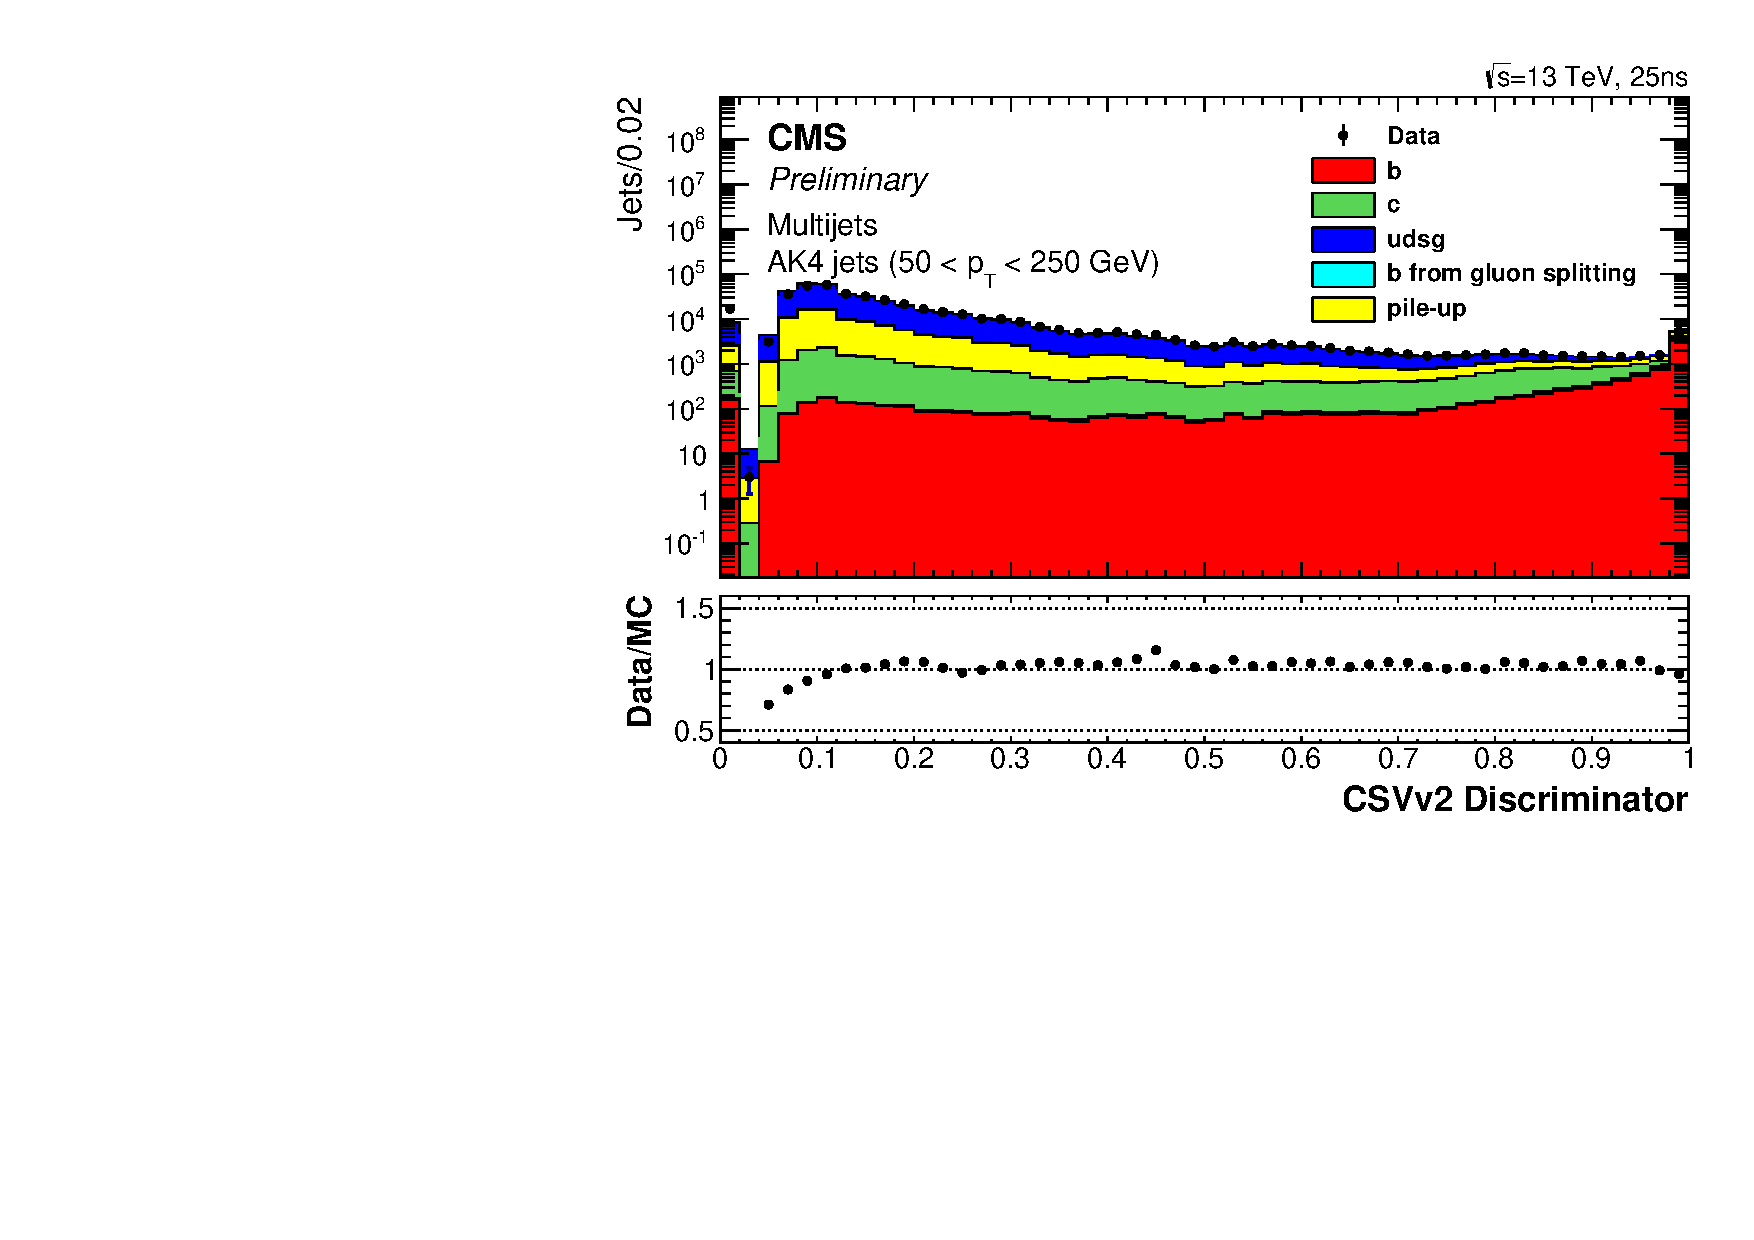
\includegraphics{figs/data-mc/ak4_pfjets_CSVIVF_Log.pdf}
\caption{The distribution of the CSVv2 algorithm's discriminator for multijet events, for $50\GeV < \pT < 250\GeV$, at $\sqrt{13\TeV}$, where the jets have been reconstructed with the anti-\kt algorithm with $R = 0.4$~\cite{CMS:2016kkf}.}
\label{fig:bTagDiscriminator}
\end{figure}

\subsection{Missing Transverse Energy}
Particles which only weakly interact with matter, such as neutrinos and some hypothesised BSM particles, escape the detector without being directly observed, but can be inferred from considering the conservation of the transverse momentum of the event.
Therefore, the missing energy in the plane transverse to the beam line, $\overrightarrow{\MET}$, is defined as the negative vector sum of the transverse momentum in the end:

\begin{equation}
\overrightarrow{\MET} = - \sum \overrightarrow{\pT} \;.
\label{eq:MET}
\end{equation}

There are several different algorithms, using differing variables and techniques, which are used in CMS analyses to determine \MET.
PF \MET, producing using the PF particles, is used in this analysis because of its high performance with \emph{Type-I} \MET corrections applied~\cite{CMS:2016ljj}.
This correction applies the jet energy corrections discussed in~\ref{} to the PF jets with $\pT >15\GeV$ which are used in calculating the \MET.
Given that the event selection for the analysis presented in this thesis uses jets with $\pT > 30\GeV$, the \emph{Type-II} corrections (discussed in detail in~\cite{Chatrchyan:2011tn}) applied to jets with $\pT < 15\GeV$ is not considered.


\chapter{Analysis Strategy and Event Selection}\label{chapter:tzq-search}
The next chapters of this thesis describe the search for the dilepton final state of a singly produced top quark in association with a Z boson (tZq) using the reconstructed proton-proton collision data at $\sqrt{13}$ collected by the CMS detector during 2016.

In contrast to previous analyses for tZq, which searched for the trilepton final state in which both the W and Z bosons decay leptonically~\cite{Sirunyan:2017kkr,Sirunyan:2017nbr}, the dilepton final state involves the W and Z bosons decaying hadronically and leptonically respectively.
This event topology presents the the main challenge for this analysis, as it is identical to the topology a large number of background processes which have cross sections many order of magnitude larger than the signal process.
Given that the signal region will inevitably be dominated by such backgrounds, it was vital that the search was designed to constrain and understand these backgrounds as much as possible.


As shown in Figure~\ref{fig:feyn_tZq}, at leading order tZq consists of a top quark, a recoil quark and a radiated Z boson.
Only

The trigger and event cleaning strategies common


The two largest irreducible 

Events with large multi-jet components, such as Z+jets and \ttbar, form the majority of the background contributions
Enriched control regions

Sources of non-prompt leptons, such as W+jets processes, 
Talk about what needs constraining - ie need for low mis-id for Z leptons, need to balance purity/efficiency for b-jets, and use of W decay products to reco top mass.


As 

\section{Trigger Strategy}\label{sec:triggerStrategy}
As the search for the tZq dilepton final state relies on the identification of the two leptons from the Z boson decay, the trigger strategy consists of selecting events from datasets identified by the presence of leptons.
Given that the signal process being searched for is dominated by background processes and will likely be limited by statistics, it is essential to reconstruct and select as many signal events as possible.
To this end both single and double lepton triggers with the lowest possible transverse momenta thresholds are considered 
to ensure that the maximum possible statistics can be obtained over the largest possible phase space.

Table~\ref{tab:triggersDatasets} lists the triggers applied to data and MC events for each channel, including the e$mu$ final state which is considered for a \ttbar enriched control region discussed in Chapter~\ref{subsec:ttbarCR}.
%Whilst the Z boson can decay into a tau anti-tau pair, despite these leptons being simulated and reconstructed in the MC, they are not considered in the event selection for this analysis due to the difficulty simulating them due to their high mass.

\begin{table}[htbp]
\topcaption {
Triggers and datasets used for each decay channel.
}
\label{tab:triggersDatasets}
  \centering
   \resizebox{\textwidth}{!}{
   \begin{tabular}{ccc}
   \hline
   \textbf{Final State} & \textbf{Dataset} & \textbf{HLT Paths}  \\
   \hline
    ee & DoubleElectron & HLT\_Ele23\_Ele12\_CaloIdL\_TrackIdL\_IsoVL\_DZ \\
    & SingleElectron &  HLT\_Ele32\_eta2p1\_WPTight\_Gsf   \\
   \hline
    $\mu\mu$ & DoubleMuon  & HLT\_Mu17\_TrkIsoVVL\_(Tk)Mu8\_TrkIsoVVL\_DZ \\  
    & SingleMuon &  HLT\_Iso(Tk)Mu24  \\  
   \hline
   e$\mu$ & MuonEG &  HLT\_Mu12\_TrkIsoVVL\_Ele23\_CaloIdL\_TrackIdL\_IsoVL(\_DZ)   \\  
          &        &  HLT\_Mu8\_TrkIsoVVL\_Ele23\_CaloIdL\_TrackIdL\_IsoVL(\_DZ)  \\
          &        &  HLT\_Mu23\_TrkIsoVVL\_Ele12\_CaloIdL\_TrackIdL\_IsoVL(\_DZ) \\
    & SingleElectron &  HLT\_Ele32\_eta2p1\_WPTight\_Gsf   \\
    & SingleMuon &  HLT\_Iso(Tk)Mu24  \\  
   \hline
 \end{tabular}}
\end{table}

\section{Event Cleaning}\label{sec:metFilters}
Following the trigger requirements, a number of filters are applied in order to so that events with beam or detector anomalies which result in anomalous \MET are not considered for use in the analysis.

\begin{itemize}
\item \textbf{Primary Vertex Filter} - ensures that the primary vertex is well reconstructed by requiring it to be within $|z| \leq 24\cm$ of the interaction point and within $d_{0} < 2\cm$ of the beam line.
\item \textbf{Beam Halo Filter} - beam halos are machine induced particles (\eg beam-gas, beam-pipe interactions) which circulate with the beam at radii up to 5m. The filter removes events with calorimeter and muon chamber energy deposits consistent with either halo particles or particle showers caused by halos interacting with the collimator blocks that used to clean halos from the beam.
\item \textbf{HBHE Noise and Isolation Filters} - removes events where anomalous noise is present in the HCAL's hybrid photodiodes or readout boxes, which registers as large isolated energy deposits which would infer the presence of large \MET, by considering the channel multiplicities, pulse shape of the readout and the neighbouring activity in the calorimeters and tracker.
\item \textbf{ECAL Trigger Primitive Filter} - the L1 trigger primitive readout can be used to estimate the energy deposited in approximately 70\% of the channels which lack regular data links and are masked out for reconstruction. As trigger the primitives have a narrower energy acceptance range than the read-out, when the energy is near their saturation energy the measured energy is likely to be underestimated, resulting in high anomalous \MET. 
%\item \textbf{ECAL Endcap SC Filters} - NOT recommended for 2016
\item \textbf{Bad Charged Hadron Filter} - removes events where a muon is not defined as a PF muon due to its low quality, but makes its way into the PF MET calculation as a charged hadron candidate.
\item \textbf{Bad Muon Filter} - removes events where a muon is defined as a PF muon, but is still has too low a quality and large \pT to be considered.
\end{itemize}

\section{Physics Objects}\label{sec:eventSelection}
This section discusses the various selection criteria this analysis applies to the physics objects which have been identified and reconstructed using the particle flow algorithm described in Chapter~\ref{chapter:data-mc}.

\subsection{Lepton Selection}
All PF electrons and muons considered must pass a set of kinematic requirements and a set identification criteria defined by CMS.
The kinematic requirements are applied to ensure that the leptons lie within detector acceptance and that their transverse momenta lies in the region where the trigger's turn-on is well described.
The identification criteria have been designed to be efficient at selecting isolated prompt leptons and rejecting leptons which have been produced non-promptly from decays from within jets or taus or from incorrectly reconstructed tracks.

Different working points are used by identification criteria defined by CMS, where the lepton selection efficiency is traded off against the purity of the leptons selected.
For both lepton flavours the ``tightest'' working point is used to select high purity collections of leptons, with the ``loosest'' working point used to veto events with any additional leptons.

\subsubsection{Electrons}\label{subsubsec:electronSelection}
For any PF electron candidate to be considered it must meet the following kinematic requirements:

\begin{itemize}
\item the \pt of the leading and subleading electrons considered must be greater than the 35\GeVc and 15\GeVc respectively.
\item electrons must have $|\eta| \leq 2.50$ to ensure that the electrons are within the ECAL acceptance.
\item as accurate reconstruction cannot be undertaken in the transition region between the ECAL barrel and endcap, electrons with $1.4442 \leq \eta \leq 1.566$ are not considered.
\item the longitudinal impact parameter, $d_{z}$, of the electron must be less than 0.10\cm in the barrel and 0.20\cm in the endcap disks.
\item the transverse impact parameter, $d_{0}$, of the electron must be less than 0.05\cm in the barrel and 0.10\cm in the endcap disks.
\end{itemize}

The \emph{tight} and \emph{veto} working points (WPs) of the \emph{cut based} identification criteria which are approximately  70\% and 95\% efficient respectively, are used to select electrons and to veto any additional electrons.
The cut based identification uses a mixture of manually set and multivariate analysis (MVA) tuned variables for btoh the barrel and endcap disks.

The manually set variables are:
\begin{itemize}
\item \textbf{$N^{missing}_{inner hits}$} - as photons which subsequently convert do not leave hits in the innermost layers of the tracker, electrons are rejected if the expected number of missing hits is exceeded.
\item \textbf{a conversion veto} - is applied for all working points, where any electron which fails the electron conversion veto is rejected.
\end{itemize}

The MVA tuned variables include:
\begin{itemize}
\item \textbf{Full $5 \times 5 \sigma_{i\eta i\eta}$} - the shower shape variable, which describes the shape of the shower in $\eta$.
\item \textbf{$\Delta \eta_{seed}$ and $\Delta \phi_{seed}$} - the distances in $\eta$ and $\phi$ between the ECAL supercluster and where the track has been extrapolated to from the primary vertex.
\item \textbf{$\frac{h}{E}$} - the ratio of hadronic to electromagnetic energy deposited in the supercluster around the crystal with the largest energy deposit.
\item \textbf{$I^{rel}_{EA}$} the relative isolation of the electron with effective area pileup alleviation for a cone size of 0.3, which is described further in Chapter~\ref{subsubsec:relIso}.
\item \textbf{$1/E - 1/p$} - the difference in the inverse energy of the ECAL supercluster and inverse track momentum, which is used to describe the energy loss 
\end{itemize}

The cuts used for the tight and veto WPs for these variables are given in Table~\ref{tab:electronCuts}.

\begin{table}[htbp]
\topcaption {
The cuts used for the tight and veto working points of the cut based identification criteria for electrons for the barrel and endcap disks.
}
\label{tab:electronCuts}
  \centering
  \resizebox{\textwidth}{!}{
% This right-aligns numbers in column, but centers them under column title.
 \begin{tabular}{ccccc}
   \hline
   \textbf{Variable} & \multicolumn{2}{c}{\textbf{Tight WP}} & \multicolumn{2}{c}{\textbf{Veto WP}}   \\
    & Barrel & Endcap & Barrel & Endcap \\
    \hline   
    Full $5\times5 \sigma_{i\eta i\eta}$ & $< 0.00998$ & $< 0.0292$ & $< 0.0115$ & $< 0.037$ \\
    $\Delta \eta_{seed}$ & $<0.00308$ & $<0.00605$ & $<0.00749$ & $<0.00895$ \\
    $\Delta \phi_{seed}$ & $<0.0816$ & $<0.0394$ & $<0.228$ & $<0.213$ \\
    $\frac{h}{E}$ & $<0.0414$ & $<0.0641$ & $<0.356$ & $<0.211$	\\
    $I^{rel}_{EA}$ & $<0.0588$ & $<0.0571$ & $<0.175$ & $<0.159$ \\
    $1/E - 1/p$ & $<0.0129$ & $<0.0129$ & $<0.299$ & $<0.15$ \\
    $N^{missing}_{inner hits}$ & $\leq 1$ & $\leq 1$ & $\leq 2$ & $\leq 3$ \\
    pass conversion veto & $\checkmark$ & $\checkmark$ & $\checkmark$ & $\checkmark$ \\
    \hline
 \end{tabular}}
\end{table}

\subsubsection{Muons}\label{subsubsec:muonSelection}
Similar to the electrons, PF muons are required to meet a set of kinematic requirements and identification and isolation criteria.

In the case of the kinematic requirements, PF muons candidates are required to:
\begin{itemize}
\item the \pt of the leading and subleading electrons considered must be greater than the 26\GeVc and 20\GeVc respectively.
\item muons must have $|\eta| \leq 2.50$ to ensure that the muon are within the acceptance of the muon systems.
\end{itemize}

The \emph{tight} and \emph{loose} identification and isolation criteria~\cite{Chatrchyan:2012xi} are used to select muons and veto any additional muons.

The tight muon criteria suppresses hadronic punch-through into the muon system and non-prompt muons, creating a high purity collection of particle flow muons.

These criteria are:
\begin{itemize}
\item muon a PF Muon and is also both a tracker and global muon.
\item $\chi^{2}/ndf$ of the global muon track fit is less than ten. 
\item at least one muon chamber is included in the global track fit.
\item that muon segments are found in at least two muon stations.
\item $d_{0} < 0.2\cm$ and $d_{z} < 0.5\cm$.
\item the muon must have at least one hit in the pixel detector.
\item hits must be present in at least six tracker layers in order to achieve a good \pT measurement.
\end{itemize}

The tight isolation cut applied to the resultant collection of tight muons is 95\% efficient, and rejects muons that have a relative isolation, with $\Delta\beta$ pileup corrections, greater than 0.15 for a cone size of 0.4.
This pileup correction for the relative isolation is described further in Chapter~\ref{subsubsec:relIso}.

Given that the loose cuts require the muon to be a particle flow muon and either a global muon or tracker muon, by definition all PF muons considered pass the loose identification cut.
The loose isolation cut is 98\% efficient and rejects muons with a relative isolation which is greater than 0.25.

\subsubsection{Lepton Isolation}\label{subsubsec:relIso}
A relative isolation variable $I^{rel}$ is used in order to:
\begin{itemize}
\item differentiate between leptons promptly produced at the primary vertex from those resulting from heavy jet or lepton decays.
\item to ensure that leptons are sufficiently separated from hadrons and photons to enable a precise momentum measurement of the lepton 
\end{itemize}

$I^{rel}$e is defined as the summed energy of all PF particles within a fixed radius cone of $\Delta R$ around the PF lepton, with the estimated neutral charged pileup contamination, $\rho$, removed, divided by the lepton \pT.

As only charged hadrons ($CH$) have associated tracks which can be used to determine if they are consistent with the primary vertex, the pileup contamination contribution from neutral hadrons ($NH$) and photons is typically estimated with one of two methods.

In the analysis presented, electrons use the $\rho$ * effective area ($rho * A_{\rm eff}$) technique using a $\Delta R$ of 0.3.
This method estimates the neutral pileup contributions by subtracting the median energy density per area of pileup contamination, $\rho$, which has been multiplied by the effective area of the electron, $A_{\rm eff}$, which is characterised as a function of the supercluster's $\eta$:

\begin{equation}
I^{rel}_{rho * A_{eff}} = \sum p_T(CH) + max (0.0, \sum E_{\rm T}(NH) + \sum E_{\rm T}(Photon) -rho*A_{\rm eff} )/p_T \\
\end{equation}\label{eq:rhoEffA}

The $\Delta\beta$ pileup mitigation method is used for muons using a $\Delta R$ of 0.4 in the analysis presented.
Using the fact that the ratio of neutral to charged hadron production in the hadronisation of pileup interactions is approximately 0.5, half of the transverse energy of charged hadrons from pileup is subtracted from the neutral hadron and photon transverse energies~\cite{Chatrchyan:2012vp}:

\begin{equation}
I^{rel}_{\Delta\beta} = \sum p_T(CH) + max (0.0, \sum E_{\rm T}(NH) + \sum E_{\rm T}(Photon) - 0.5 * \sum E_{\rm T}(PU))/p_T \\
\end{equation}\label{eq:deltaBeta}

\subsubsection{Z Boson Candidate Invariant Mass Requirements}
The presence of a Z boson in the final state requires that two leptons selected must be consistent with a Z boson decay.
Therefore, the leptons must have the same flavour and opposite charge and an invariant mass within 20\GeVcc of the known Z mass.
%This mass window was determined on the basis of 
%including sufficient signal events 

\subsection{Jet, b-tagging and W Boson Candidate Requirements}
\subsubsection{Jet Requirements}
Jets are considered from the PF jet collection which reconstructs jets using the \emph{anti-\kt} algorithm with R = 0.4 with charged hadrons originating from \PU vertices excluded from clustering.
Following identification, the jet energy corrections are applied as described in Chapter~\ref{subsubsec:JECs}.

Jets are considered in the analysis if they have a $\pT > 30\GeVc$, are within $|\eta| < 4.7$ and meet the \emph{loose} working point jet identification criteria developed by CMS.
In addition, selected leptons (electron or muon) which lie within a cone of $\Delta R = 0.4$ of a selected jet are not considered to be a prompt leptons and instead part of the jet in question.

The loose jet ID was designed to reject the majority of the fake tracks produced from detector and/or electronics noise whilst maintaining a high selection efficiency for real jets by requiring all jets to have part of their energy deposited in both the ECAL and HCAL and be composed of more than one particle.

\editComment{Necessary to spell this out? Or comment out ...}
The loose jet identification criteria are as follows:

for jets with $\eta \leq 2.70$ the loose ID criteria are:
\begin{itemize}
\item the fraction of the jet energy from both neutral electromagnetic particles in the ECAL and neutral hadronic particles in the HCAL is less than $0.99$.
\item at least two constituent particles are present.
\end{itemize}

with these applying in addition for $\eta \leq 2.40$:
\begin{itemize}
\item the fraction of the jet energy from charged electromagnetic particles in the ECAL is less than $0.99$ and greater than 0.0 for charged hadronic particles in the HCAL.
\item at least one charged particle is present.
\end{itemize}


for jets with $ 2.70 \leq \eta \leq 3.0$ the loose ID criteria are:
\begin{itemize}
\item the fraction of the jet energy from neutral electromagnetic particles in the ECAL is greater than than $0.01$ and less than $0.98$ for neutral hadronic particles in the HCAL.
\item at least three neutral particles are present.
\end{itemize}

and for jets with $\eta > 3.0$ the loose ID criteria are:
\begin{itemize}
\item the fraction of the jet energy in the ECAL that is from neutral electromagnetic particles is less than $0.90$.
\item at least eleven neutral particles are present.
\end{itemize}

\subsubsection{b-tagging}
The CSVv2 tagging algorithm described in Chapter~\ref{subsec:objReco-bJets} is used to tag jets, with a working point (WP) cut applied to the b-tag discriminator.
If the value of a jet's discriminator exceeds that of the Medium WP and has $|\eta| < 2.40$, the jet is considered to be a b-jet.
From the \emph{Loose}, \emph{Medium} and \emph{Tight} WPs defined by CMS~\cite{Sirunyan:2017ezt}, as given in Table~\ref{tab:bTagWPs} in Chapter~\ref{subsec:objReco-bJets}, the Medium WP was chosen as it provided the optimum performance in terms of providing as large statistics as possible for the signal process without too great a compromise on the purity of the selection.

\subsubsection{W Boson Candidate Invariant Mass Requirements}
In contrast to the previous tZq searches where the W boson decays into a lepton and its associated antineutrino, the W boson in the dilepton final state decays hadronically, allowing for the top quark to be fully reconstructed.
The W boson candidate is constructed by considering each possible pair of jets, with the pair with a dijet invariant mass closest to the known W boson mass of 80.4\GeVcc being chosen as the W candidate.
The leading b-jet however, is excluded from consideration as the hardest b-jet is assumed to be produced from the decay of the top quark. 

\subsection{\MET}\label{subsec:met}
Whilst the signal region does not explicitly cut on \MET, it is used in one of the Z+jets control regions, described in Chatper~\ref{subsec:zPlusJetsCR}, and in the boosted decision tree, discussed in Chapter~\ref{subsec:bdt}, in order to discriminate against backgrounds such as \ttbar which do feature significant amounts of \MET.

\section{Data and MC Simulation Samples}\label{sec:samples}
The analysis uses proton-proton collision data at $\sqrt{13}$ in 2016, considering events in the double lepton and single lepton datasets where the double and single lepton triggers respectively have fired, using the strategy described in Chapter~\ref{sec:triggerStrategy}.

Table~\ref{tab:mcList} lists the MC samples used to simulate the signal and background processes that were considered, included information on the number of events generated, their cross sections and the order in perturbative accuracy in QCD to which the generators calculated the processes.

Table~\ref{tab:theorySampleList} lists the additional dedicated simulated samples that were used to determine the impact of a number of theoretical uncertainties, which are discussed further in Chapter~\ref{sec:theorySysts}.

The hadronisation of all the MC samples considered was done using PYTHIA 8.

\begin{table}[htbp]
\topcaption {
The MC processes and their associated total number of events, cross sections and generators (and order in perturbative QCD accuracy they are calculated to), considered for the search for tZq in the dilepton final state. Both generators considered for the Z+jet background are also listed below.
}
\label{tab:mcList}
  \centering
  \resizebox{\textwidth}{!}{
% This right-aligns numbers in column, but centers them under column title.
 \begin{tabular}{cccc}
   \hline
   \textbf{MC process} & \textbf{Events} & \textbf{Cross section (pb)} & \textbf{Generator (Order)}   \\
   \hline
   tZq  & 14.5M & 0.0758  & aMC@NLO (NLO) \\
   \hline
   tHq  & 3.5M & 0.07462  & Madgraph (LO) \\
   \hline
   tWZ/tWll  & 50K & 0.01104  & Madgraph (LO) \\
   \hline
   t tW-channel & 7M & 35.85 & POWHEG (NLO) \\
   $\overline{\text{t}}$ tW-channel & 6.9M & 35.85 & POWHEG (NLO) \\
   \hline
   t s-channel & 2.9M & 10.32 & aMC@NLO (NLO) \\
   \hline
   t t-channel & 67.2M & 136.02 & POWHEG (NLO) \\
   $\overline{\text{t}}$ t-channel & 38.8M & 80.95 & POWHEG (NLO) \\
   \hline
   \ttbar & 77.1M & 831.76 & POWHEG (NLO) \\
   \hline
   \ttbarZ $\rightarrow$ ll$\nu\nu$ & 13.9M & 0.2529   & aMC@NLO (NLO) \\
   \ttbarZ $\rightarrow$ qq & 749K & 0.5297   & aMC@NLO (NLO) \\
   \hline
   \ttbarW $\rightarrow$ l$\nu$ & 5.3M & 0.2001   & aMC@NLO (NLO) \\
   \ttbarW $\rightarrow$ qq & 833K & 0.405  & aMC@NLO (NLO) \\
   \hline
   \ttbarH $\rightarrow$ bb & 3.8M & 0.2942 & POWHEG (NLO) \\
           $\rightarrow$ non bb & 4.0M & 0.2123 & POWHEG (NLO) \\
   \hline
   W+jets & 24.1M & 61526.7 & aMC@NLO (NLO) \\
   \hline
   Z+jets ($m_{Z} \geq 50\GeVcc $ & 146M & 5765.4 & Madgraph (LO) \\
   Z+jets ($10 \GeVcc \leq m_{Z} < 50\GeVcc$ & 35.3M & 18610.0 & Madgraph (LO) \\
   \hline
   Z+jets ($m_{Z} \geq 50\GeVcc $ & 151M & 5765.4 & aMC@NLO (NLO) \\
   Z+jets ($10 \GeVcc \leq m_{Z} < 50\GeVcc$ & 106M & 18610.0 & aMC@NLO (NLO) \\
   \hline
   WW $\rightarrow$ l$\nu$qq & 9.0M & 49.997  & POWHEG (NLO) \\
      $\rightarrow$ ll$nu\nu$ & 2.0M & 12.178 & POWHEG (NLO) \\
   \hline
   WZ $\rightarrow$ l$\nu$qq & 24.2M & 10.73 & aMC@NLO (NLO) \\
      $\rightarrow$ llqq & 26.5M & 5.606 & aMC@NLO (NLO) \\
      $\rightarrow$ lll$\nu$ 1.9M & 5.26 & aMC@NLO (NLO) \\
   \hline
   ZZ $\rightarrow$ ll$\nu\nu$ & 8.8M & 0.5644 & POWHEG (NLO) \\
      $\rightarrow$ llqq & 15.3M & 3.222 & aMC@NLO (NLO) \\
      $\rightarrow$ llll & 10.7M & 1.204 & aMC@NLO (NLO) \\
   \hline
   WWW & 240K & 0.2086 & aMC@NLO (NLO) \\
   \hline
   WWZ & 250K & 0.1651 & aMC@NLO (NLO) \\
   \hline
   WZZ & 247K & 0.05565 & aMC@NLO (NLO) \\
   \hline
   ZZZ & 249K & 0.01398 & aMC@NLO (NLO) \\
   \hline
   
 \end{tabular}}
\end{table}

\begin{table}[htbp]
\topcaption {
The dedicated MC samples used to determine the impact of theoretical uncertainties, including the associated total number of events, cross sections and generators (and order in perturbative QCD accuracy they are calculated to), considered for the search for tZq in the dilepton final state.
}
\label{tab:theorySampleList}
  \centering
 \resizebox{\textwidth}{!}{
 \begin{tabular}{cccc}
   \hline
   \textbf{MC process} & \textbf{Events} & \textbf{Cross section (pb)} & \textbf{Generator (Order)}   \\
   \hline
   tZq scale up & 6.9M & 0.0758  & aMC@NLO (NLO) \\
   tZq scale down & 7.0M & 0.0758  & aMC@NLO (NLO) \\
   \hline
   t tW-channel scale up & 998K & 35.85 & POWHEG (NLO) \\
   t tW-channel scale down & 994K & 35.85 & POWHEG (NLO) \\
   $\overline{\text{t}}$ tW-channel scale down & 1.0M & 35.85 & POWHEG (NLO) \\
   $\overline{\text{t}}$ tW-channel scale down & 999K & 35.85 & POWHEG (NLO) \\
   \hline
   t t-channel scale up & 5.7M & 136.02 & POWHEG (NLO) \\
   t t-channel scale down & 5.9M & 136.02 & POWHEG (NLO) \\
   t t-channel matching up & 6.0M & 136.02 & POWHEG (NLO) \\
   t t-channel matching down & 6.0M & 136.02 & POWHEG (NLO) \\
   $\overline{\text{t}}$ t-channel scale up & 4.0M & 80.95 & POWHEG (NLO) \\
   $\overline{\text{t}}$ t-channel scale down & 3.9M & 80.95 & POWHEG (NLO) \\
   $\overline{\text{t}}$ t-channel matching up & 4.0M & 80.95 & POWHEG (NLO) \\
   $\overline{\text{t}}$ t-channel matching down & 4.0M & 80.95 & POWHEG (NLO) \\
   \hline
   \ttbar ISR up & 156.5M & 831.76 & POWHEG (NLO) \\
   \ttbar ISR down & 149.8M & 831.76 & POWHEG (NLO) \\
   \ttbar FSR up & 152.6M & 831.76 & POWHEG (NLO) \\
   \ttbar FSR down & 156.0M & 831.76 & POWHEG (NLO) \\
   \ttbar matching up & 58.9M & 831.76 & POWHEG (NLO) \\
   \ttbar matching down & 58.2M & 831.76 & POWHEG (NLO) \\
   \hline   
 \end{tabular}}
\end{table}

\section{Simulation Corrections}\label{sec:simCorrections}
Simulation is unable to fully recreate all the effects observed in data, either because certain parameters are not precisely known or cannot be be calculated.
To account for these discrepancies, corrective scale factors are used to reweight MC on a per event basis.
Such scale factors are usually derived as a function of \pt and $\eta$ so as to account for the variation of the detector response in both.
These corrections are used to correct simulation for lepton identification, isolation and reconstruction efficiencies, b-tagging efficiencies, the poor modelling of pileup in simulation, and the detector resolutions observed in data.

\editComment{add SF distributions in appendix? Noticed others do this...}

\subsection{Miscalibrated Tracker APV}\label{subsec:hipEffect}
During the first half of data taking in 2016 the silicon strip detector suffered from instantaneous luminosity dependent  hit finding inefficiencies, particularly in high occupancy regions, due to saturation in the pre-amplifier in the front end electronics~\cite{Fiori:2016ebh}.
This issue was resolved by changing the configuration of the electronics.
While the affected part of the dataset has been reprocessed to mitigate the impact on the quality of the data taken, there is still a negative impact on the detector efficiency for objects that rely upon highly efficient tracking data.
This is accounted for by the weighting of events appropriately when the scale factors are produced, either centrally by CMS or those derived for the analysis (\ie the trigger scale factors), so that a single scale factor is applied to a simulated event.

%In most cases, centrally produced scale factors are derived for the whole of the 2016 dataset to account for this, but 
%for muons they were provided for both the affected and unaffected parts of the dataset separately.
%Consequently, the muon scale factors were weighted according to the luminosity they corresponded to before their application to simulation.
%Similarly, the muon trigger scale factors that were derived were also produced 

\subsection{Lepton Efficiency}\label{subsec:leptonRecoSFs}
The identification, isolation and reconstruction efficiencies of leptons are calculated using measurements of $Z \rightarrow l^{+} l ^{-}$ events with the \emph{tag-and-probe} method~\cite{CMS:2008rxa}.
Using events within a dilepton invariant mass window to ensure a high purity, from this large statistics lepton sample, the method ``tags'' and ``probes'' the leptons where one has passed a tight and the other a loose selection criteria.
For source of each efficiency and lepton flavour, the efficiency is given as the fraction of events where the probe leptons passed the relevant selection criteria.
This methodology is used to create corrective scale factors for each component and these are multiplicatively applied to each leptons' event weight as functions of their \pt, $\eta$, and flavour.

The trigger efficiency of electrons and muons is calculated using a method which considers events that pass the lepton selection criteria in the signal region~\ref{sec:signalRegion} and which are selected by triggers which are weakly correlated (also known as cross triggers) with the triggers used in the analysis~\cite{Khachatryan:2016kzg}.
From this collection of events, the number of events that pass and fail the analysis triggers are counted to produce the trigger efficiency:

\begin{equation}
\epsilon_{trigger} = \frac{N_{X triggers + lepton triggers}}{N_{X triggers}} \\
\end{equation}

where $N_{X trigger}$ is the number of events which have passed the lepton selection criteria and the cross triggers, and $N_{X triggers + lepton triggers}$ is $N_{X trigger}$ and the number of events which have also passed the lepton triggers.

As the triggers requirements are applied to both simulated and data events, a scale factor of the ratio of the trigger efficiency in data and in simulation is applied to the event weight in simulation.

%For the scale factors derived for the ee and e$\mu$ channels, a constant scale factor was found to be sufficient to account for the differences between data and siulation.
%In the case of the $\mu\mu$ channel however, the scale factor was produced as a function of both \pt and $\eta$ due to the trigger turn-on curve in data being impacted by the miscalibrated tracker APV (as discussed in Chapter~\ref{subsec:hipEffect}.

\subsection{Lepton Energy Corrections}\label{subsec:leptonEnergyCorrections}
\subsubsection{Electron Regression and Energy Scale and Smearing Corrections}
Two types of energy corrections which have been produced by the CMS EGM POG are applied to electrons and photons, energy regression and energy scale and smearing corrections.
These corrections are applied to both MC simulation and data and are used to improve the electron resolution obtained and to resolve the observed discrepancies between them.

Using simulation for tuning, energy regression obtains the best possible energy resolution by using the detector information to correct the reconstructed object energy.
The disagreement between data and MC is resolved by scaling the data energy to the MC energy scale and smearing the MC so that it has the same energy resolution as data. 

These corrections are pre-applied onto the PF electron collections used.

\subsubsection{Rochester Corrections}
The muon momentum scale and resolution correction methods developed by the University of Rochester~\cite{rochester}, known as \emph{Rochester Corrections}, are used to remove any muon momentum bias from any detector misalignment, reconstruction or uncertainties in the magnetic field for both MC and data.
These corrections are derived with high \pt ($> 20\GeVc$) muons from Z $ \rightarrow \mu\mu$ decays using a two step method, where the muons are binned in charge, $\eta$ and $\phi$.
The first step requires the mean inverse transverse momenta of the muons reconstructed from data and simulation to be the same as the corresponding values from a perfectly aligned detector.
These corrections are tuned in the second step by using the $M_{\mu^{+1}\mu^{-1}}$ peak for a perfectly aligned detector to calibrate the corrections.
This removes any sensitivity to detector efficiencies or physics modelling.

The Rochester Corrections are applied to each muon an event weight that is a function of the muon's charge, \pt, $\eta$ and $phi$.

\subsection{Jet Energy Corrections}\label{subsec:jesjer}
As described in Chapter~\ref{subsubsec:JECs}, the JECs are applied to account for the non-uniform response in \pT and $eta$ of the detector by comparing the differences between the generator level and detector level responses.

In addition to these corrections, as the Jet Energy Resolution (JER) observed in data is approximately 10\% poorer than that in observed simulation, the 4-vectors of simulated jets are smeared as functions of generator level and reconstructed \pt and $\eta$ to account for this~\cite{Khachatryan:2016kdb}.

\subsection{b-tagging Efficiency}\label{subsec:btagEff}
The B-Tag and Vertexing (BTV) Physics Object Group measures the b-tagging efficiency and misidentification rates for b and light flavoured jets in data and MC simulation (multijet and \ttbar) of the algorithms which they support~\cite{Sirunyan:2017ezt}.
From these measurements b-tagging efficiency scale factors are produced and provided for analysts to apply to simulated events to correct differences observed between data and simulation.
These scale factors, as functions of the jet flavour, \pT and $\eta$, to alter the weight of the selected MC events.
This methodology was chosen as it involves only changing the weight of the selected MC events which, unlike other methods, avoids events migrating into different b-tag multiplicity bins and having events with potentially undefined variables such as the top mass.

\subsection{\PU Modelling}\label{subsec:puSF}
It is challenging to model variations in the number of \PU interactions that result from the changing LHC conditions.
Therefore MC events are reweighted as a function of the number of primary vertices so that the PU interactions simulated are resembles what is observed in data.

The \PU SF is determined as a function of the number of primary vertices, $n_{PV}$, present by comparing $n_{PV}$ in minimum bias data over the running period considered to $n_{PV}$ for simulated events.

\subsection{Top quark \pt}
A scale factor is applied to \ttbar MC as a function of the top's and anti-top's generator level transverse momenta to account for the \pt spectra of top quarks in data being significantly softer than that predicted by LO and NLO precision MC simulation~\cite{Khachatryan:2015oqa}.

\section{Signal Region}\label{sec:signalRegion}
The signal enriched region event selection was designed select signal events with a high efficiency whilst rejecting as much of the background process as possible.
To ensure that the leptons selected are promptly produced and are of a high purity, exactly two leptons of the same flavour which pass the tight identification and isolation criteria, wi


As the tZq dilepton final state is distinguished by the presence of exactly two leptons from the Z boson decay, being able to identify these isolated prompt leptons with a high efficiency and a low misidentification rate is essential.

To ensure a 
Whilst additional jets could be produced by further gluon splitting, in practice 

No \MET cut is applied in the signal region event selection despite there being no \MET directly produced by the signal process.
This decision was taken as \MET was anticipated to be a useful variable the multivariate analysis (discussed in Chapter~\ref{sec:mvas}) that could be used to discriminate against background processes such as \ttbar.

\section{Control Regions}\label{sec:controlRegions}
In any high energy particle physics analysis, accurate modelling of the background processes is essential in order to be able to make a measurement.
As the main challenge in searching for the dilepton final state of tZq is that the signal region is dominated by background processes, it particularly important to ensure that the background processes are accurately modelled in simulation.
In order to confirm whether or not simulation adequately describes the data and thus if data-driven estimations are required instead, background enriched control regions which are topologically similar and orthogonal to the signal region are used for the two largest background processes are defined.
The same trigger, event cleaning, number of oppositely charged leptons, number of jets required and W and Z boson mass selection criteria are applied to the control regions so that they occupy a topologically similar phase space to the signal region.
Where required, these control regions are extrapolated to provide a data-driven estimation of the background in the signal region as discussed in Chapter~\ref{sec:dataDrivenBackground}.

\subsection{Z+jets Background Control Regions}\label{subsec:zPlusJetsCR}
Despite the majority of such events being rejected by the signal region criteria, given the large cross section for Z+jets, the remaining events from this process dominate the signal region to form the single largest background.
Given the size of this background and the difficulties in accurately modelling higher order contributions from QCD processes, it is essential to ensure that both the normalisation and modelling of the jets for this background are well described.

Initially a high statistics Z+jets enriched control region was defined by requiring that none of the jets present are b-tagged, in contrast to the one to two required for the signal region, as the majority of the jets 
Given the large cross section and that the vast majority of the jets produced by the Z+jets process are light jets, whilst the top quarks in \ttbar, the second largest background, predominately decay into b quarks, this produces a high purity region with large statistics.

Despite the good description of the jet multiplicity and jet \pT shapes in this control region, discussed in depth in Chapter~\ref{subsec:zPlusJetsEstimation}, as the kinematics of b-tagged jets differs from light jets, the topology may 

Therefore an alternative Z+jets enriched control region was defined by requiring same b-jet selection (one to two b-jets) as the signal region and a \MET cut of 50\GeV is applied to suppress \ttbar where significant quantities of \MET are expected from the leptonically decaying W bosons.

The application of both of these control regions is discussed in Chapter~\ref{sec:dataDrivenBackground}.

\subsection{\ttbar Background Control Region}\label{subsec:ttbarCR}
\ttbar events form the second largest background process, where events with two leptons produced from W bosons decaying having an invariant mass which is compatible with the Z boson mass window in the being selected in the signal region.
The selection criteria for the \ttbar control region differs from the signal region definition defined in Chapter~\ref{sec:signalRegion}, by requiring that the two oppositely leptons selected to have different flavours (\ie one is an electron and the other a muon).
%The electron and muon \pt thresholds are modified from those given in Chapters~\ref{subsubsec:electronSelection} and~\ref{subsubsec:muonSelection} as the leading lepton \pt thresholds of the HLT paths considered for the e$\mu$ final state, as given in Chapter~\ref{sec:triggerStrategy}, differ from those for the same flavour final states.

As the branching ratio for a W boson (produced by the top quark and anti-top quark decays) to decay into either an electron or muon is the same, this produces a \ttbar enriched background control region which is topologically similar to the \ttbar contributions in the signal region. 

\begin{table}[htbp]
\topcaption {
The event yields after the selection criteria have been applied for the \ttbar control region.
}
\label{tab:ttbarCR}
  \centering
% This right-aligns numbers in column, but centers them under column title.
 \begin{tabular}{cc}
   \hline
   \textbf{MC process} & \textbf{$e\mu$}  \\
   \hline
   tZq & 1.709\\
   \ttbar & 11778.461 \\
   Z+jets & 80.9921\\
   tW & 488.632\\
   Other & 166.200\\
   \hline
   Data & 12509.0 \\
   Total MC & 12515.995 \\
   \hline
 \end{tabular}
\end{table}

%\section{Blinding}\label{sec:blinding}


\chapter{Background Estimation}\label{chapter:bkg}
Despite 

\section{Data-driven Background Esimation}\label{sec:dataDrivenBackground}
\subsection{Non-Prompt Leptons}\label{sec:NPLs}
Backgrounds which involve decays into lepton + jets and where at least one jet is incorrectly reconstructed as a lepton (predominately electrons) or a lepton from the decay of heavy quarks (predominately muons), which pass the lepton selection and isolation criteria, are estimated with data.

The estimation of this background uses the same methodology as when performing top quark pair production~\cite{CMS:2016syx} and same-sign SUSY searches~\cite{CMS:2015vqc}.
The vast majority of the same-sign event yields found are the result of non-lepton and charge misidentified leptons, with some contribution from prompt leptons.
As these backgrounds are independent of the charge of the lepton pairs, it is expected that the nominal (opposite-sign) sample would have a similar contribution \cite{CMS:2015vqc}.

To estimate this contribution of opposite-sign non-prompt leptons in data, the same-sign event yields with the expected prompt-lepton contribution subtracted, is multiplied by a ratio of opposite-sign over same-sign non-prompt lepton events taken from MC.

The method requires that the same-sign control region established uses the same selection criteria as the nominal signal region, albeit with same-sign lepton pairs instead of opposite-sign ones.
This control region is dominated by non-lepton lepton events, but also contains contributions from prompt lepton events, charge misidentification and real same-sign pairs.

This data driven estimate is obtained using the following equation:

\begin{equation}
 N_{data}^{OS non-prompt} = (N_{data}^{SS} - N^{SS}_{real + mis-ID}).\frac{N_{MC}^{OS non-prompt}}{N_{MC}^{SS non-prompt}}
\end{equation}

where $N_{data}^{SS}$ is the total number of same sign events observed in data, $N^{SS}_{real + mis-ID}$ is the expected number of real same-sign events and events with charge misidentification and $N_{MC}^{OS non-prompt}$ and $N_{MC}^{SS non-prompt}$ the number of opposite-sign and same-sign non-prompt leptons observed in MC used to appropriately scale the estimate.

This ratio of MC opposite-sign over same-sign events is referred to as R, and is calculated using generator level information from reconstructed objects which have matched to a generator level particle. R is calculated from the W + jets, \ttZ and \ttW leptonic decaying, and single top MC samples with sufficient statistics given that these processes are expected to be the predominant source of non-prompt leptons for this analysis. 

\begin{table}[!htbp]
\centering
\begin{tabular}{| l |  c |  c |  c |  c |  c |}
\hline
Source &  $ee$ & $\mu\mu$ & Combined \\ 
\hline
\ttbar (SS): & a$\pm$b &  c $\pm$d & e$\pm$f    \\
Z + jets (SS): & a$\pm$b &  c$\pm$d & e$\pm$r    \\
Single Top (SS): & a$\pm$b & c$\pm$d & e$\pm$r    \\
VV (SS): & a$\pm$b & c$\pm$d & e$\pm$f    \\
ttV (SS): & a$\pm$b &  c$\pm$d & e$\pm$f    \\ 
\hline
Total background (SS): & a$\pm$b & c$\pm$d & e$\pm$f   \\ 
Data: & a$\pm$b & c$\pm$d & e$\pm$f    \\ 
\hline
SS data (bkg): & a$\pm$b & c$\pm$d & e$\pm$f \\
\hline
Non-prompt (SS): & a$\pm$b & c$\pm$d & e$\pm$f \\
Non-prompt (OS): & a$\pm$b & c$\pm$d & e$\pm$f \\
R (OS/SS): & a$\pm$b & c$\pm$d & e$\pm$f \\
\hline
Non-prompt estimation: & a$\pm$b & c$\pm$d & e$\pm$f \\
\hline
\end{tabular}
\caption{Non-prompt lepton estimation following all selection cuts}
\label{tab:fakeLeptonYields}
\end{table}

\subsection{Z+jets background}\label{subsec:zPlusJetsEstimation}
Madgraph - normalises well but poor jet multiplicity
aMC@NLO - bad normalisation, but good higher jet multiplicity description

\subsection{\ttbar background}\label{subsec:ttbarEstimation}


\section{Multivariate Analysis Techniques}\label{sec:mvas}
Single top 
\subsection{Boosted Decision Trees}\label{subsec:bdt}

BDT implemented in XGBoost Library
BDT features and hyperparameters chosen separately for ee and mumu channels
Features chosen using recursive feature elimination
Hyperparameters are selected by using a Gaussian process to optimise the classifier’s performance
hyperparameters = learning rate, n-estimators, max tree depth
feature = input variable

\subsubsection{BDT input variables}
Variables chosen

\begin{table}[htbp]
\topcaption { The name and descriptions of the variables chosen by recursive feature elimination to be used as input to the BDT to discriminate between potential tZq signal events and the dominant.
}
\label{tab:bdtVariables}
  \centering
% This increases column spacing.
\resizebox{\textwidth}{!}{
% This right-aligns numbers in column, but centers them under column title.
\begin{tabular}{cccc}
   \hline
   \textbf{Variable} & \textbf{Description} & \textbf{$ee$} & \textbf{$\mu\mu$} \\
   \hline
    bTagDisc & b-tag discriminator of the leading b-tagged jet & $\checkmark$ & $\checkmark$ \\
    fourthJetPt & \pt of the fourth jet & $\checkmark$ & $\checkmark$ \\
    jetHt & Total \HT of every jet & $X$ & $\checkmark$ \\
    jetMass & Total mass of every jet & $\checkmark$ & $\checkmark$ \\
    jjDelR & $\Delta R$ between the leading jets & $\checkmark$ & $\checkmark$ \\
    leadJetEta & $\eta$ of the leading jet & $\checkmark$ & $\checkmark$ \\
    leadJetPt & \pt of the leading jet & $\checkmark$ & $\checkmark$ \\
    met & \met & $\checkmark$ & $\checkmark$ \\
    secJetPt & \pt of the second jet & $\checkmark$ & $\checkmark$ \\
    thirdJetPt & \pt of the third jet & $\checkmark$ & $\checkmark$ \\
    topMass & $m_{top}$ & $\checkmark$ & $\checkmark$ \\
    totHtOverPt & Total \HT divided by total \pt & $\checkmark$ & $\checkmark$ \\
    wPairMass & $m_{W}$ & $\checkmark$ & $\checkmark$ \\
    wQuark2Eta & $\eta$ of the second W boson candidate jet & $X$ & $\checkmark$ \\
    wwdelR & $\Delta R$ between the W boson candidate jets & $\checkmark$ & $X$ \\
    zEta & $\eta$ of the Z boson & $X$$ & $\checkmark$ \\
    zHt & \HT of the Z boson & $\checkmark$ & $\checkmark$ \\
    zMass & $m_{Z}$ & $\checkmark$ & $\checkmark$ \\
    zTopDelR & $\Delta R$ between the Z boson and top quark & $X$ & $\checkmark$ \\
    zjminR & Minimum $\Delta R$ between the Z boson and a jet & $\checkmark$ & $\checkmark$ \\
    zlb1DelR & $\Delta R$ between the Z boson and leading b-tagged jet & $\checkmark$ & $X$ \\
   \hline
 \end{tabular}}
\end{table}

\editComment{LOTS of PLOTS of the input variable distributions}

\subsection{BDT Training and Output}
Each sample of events for each process considered is split into a training and testing sample.
\chapter{Systematic Uncertainties}\label{chapter:systematics}
%%% Intro
In order to make a meaningful and robust measurement, it is vital to understand the and control the sources of systematic uncertainties associated with the physics analysis.
This is particularly important for the search for tZq where the low cross section of the signal process against a background dominated signal region requires ... 

%%% Sources
These sources of uncertainty either originate from experimental or theoretical uncertainties and typically influence the result in one of two ways:
\begin{itemize}
\item \textbf{Rate or normalisation uncertainties} impact the number of events present and thus influence the  normalisation of the distributions considered.
\item \textbf{Shape or scale factor uncertainties} impact the shape of the distributions as they involve the scaling of individual events as a function of their kinematics in order to correct inconsistencies between simulation and data.
\end{itemize}

These uncertainties, as well as the statistical uncertainties arising from the size of the simulated samples available, are treated as nuisance parameters in the statistical fit model which is discussed in~\ref{chapter:results}.

\section{Experimental Uncertainties}
\subsection{Jet Energy Corrections}
The Jet Energy Corrections group also provides the uncertainties associated with the JES and JER they determine, discussed in Chapters~\ref{subsubsec:JECs} and~\ref{subsec:jesjer}, are determined by the Jet Energy Corrections group~\cite{Khachatryan:2016kdb}. 

The impact that the JES has on the jet kinematics is evaluated by varying the corrective JES up and down by a standard deviation.
The uncertainty associated with the JER smearing is accounted for by varying the smearing factor up and down by the associated statistical uncertainty.
Recently the uncertainties associated with the JER have been updated during the reprocessing of the 2016 dataset to include the systematic uncertainties in addition to the statistical uncertainties.
At the time of writing this thesis, these reprocessed samples and the impact of the revised total JER uncertainties has not been propagated through the analysis.

The impact of the uncertainties associated with both the JES and JER on the \MET are accounted for by propagating the JEC uncertainties through to the \MET and evaluating the impact they have.

\subsection{Pileup Reweighting}
The uncertainty associated with the primary vertex distributions used in the \PU reweighting is determined by varying the expected minimum bias cross section used in simulation $\pm X%$ in order to ascertain the impact of greater or lesser amounts of \PU on the analysis.

\subsection{Parton Density Functions}\label{subsec:pdfSysts}
%%Discussion of what PDFs are, is given in an earlier chapter 
The impact of the PDF uncertainties are evaluated according to the PDF4LHC recommendations~\cite{Butterworth:2015oua}, where they are estimated as the standard deviation of the weights of the nominal and the variations of the PDF set.

For almost all of the MC samples considered, this is achieved by considering the nonimal event weight and one hundred alternative PDF weights which are stored as per-event weights in the LHE 
event header for almost all of the MC samples considered.

The single top tW-channel samples are the exception to this as at the time of their generation it was not possible to generate per-event weights to account for the PDF variations for this process.
Therefore, the LHAPDF (Les Houches Accord Parton Distribution Function) library is used to access both the nominal PDF weight and 50 eigenvalues from the NNPDF3.0 set to provide one hundred alternative event weights to be evaluated.

\subsection{b-tagging Uncertainties}
The uncertainties associated with the b-tagging scale factors described in Chapter~\ref{subsec:btagEff} are obtained by varying their value by $\pm 1\sigma$, as calculated by the BTV POG.

\subsection{Non-prompt Lepton Contributions}
As this data-driven estimate of the instrumental backgrounds should have no dependence on either the lepton flavour or selection cuts, the variation of the ratio of opposite-sign over same-sign events as a function of the lepton flavour and the cut level was considered to be well accounted for by a 30\% rate uncertainty.

\subsection{Luminosity Uncertainties}
CMS uses the pixel detector, DTs, HF, the Fast Beam Conditions Monitor and Pixel Luminosity Telescope to monitor and measure the instantaneous and integrated luminosity.
During Run 2, the primary offline luminosity measurements made by the CMS Luminosity Group used the pixel detector using the Pixel Cluster Counting (PCC) method due its stability over time for up an average \PU of 150 and the high precision results obtained with it during Run I.
The PCC algorithm is able to achieve such a precision by measuring the instantaneous luminosity through the number of pixels present. 
This is possible as the probability of pixel hit belonging to multiple tracks is very small due to the very low occupancy of the detector, inferring that the number of pixel hits are linearly proportional to the number of interactions during a bunch crossing~\cite{CMS:2017_lumi}.

Using Van der Meer (VdM) scans during dedicated LHC runs to calibrate the absolute luminosity scale calibrations of the detectors~\cite{vanderMeer:1968zz}.
The overall uncertainty in the integrated luminosity collected by CMS in 2016 was estimated to be 2.5\%~\cite{CMS:2017_lumi}.

%The MC events produced are weighted by a scale factor in order to correctly normalise them with respect to the data they are compared against.
%This normalisation scale factor is given by:
%\begin{equation}
%SF_{dataset} = \frac{\pazocal{L} \sigma}{N_{MC}^{Events}}
%\end{equation}
%where $\pazocal{L}$ is the amount of total integrated luminosity considered in the data used, $\sigma$ the cross section of the MC sample considered and $N_{MC}^{Events}$ is number of simulated events considered for the process.

\subsection{Lepton Efficiencies}
The uncertainties associated with the lepton identification, isolation and reconstruction efficiency scale factors discussed in Chapter~\ref{subsec:leptonRecoSFs} are varied +/- 1 sigma.

%The uncertainty associated with the lepton trigger efficiencies are calculated using 
%The conservative method of Clopper-Pearson intervals~\cite{Cousins:2009kz} was used to determine the uncertainities associated with the trigger scale factors used.

%The potential correlations between the cross triggers and lepton triggers used are one source of systematic uncertainty.
%If both triggers are independent, then the efficiency of fulfilling both trigger selections can be expressed as:
%\begin{equation}
%\epsilon_{X + lepton triggers} = \epsilon_{X triggers} \times \epsilon_{lepton triggers}
%\label{eq:triggerCorrelation}
%\end{equation}
%
%and if both trigger selections are uncorrelated, then the ratio of the left and right hand sides ($\alpha$) of Equation~\ref{eq:triggerCorrelation} would be 1.
%Table~\ref{tab:triggerAlpha} shows that the values of $\alpha$ determined for each channel only differ slightly from 1.
%\begin{table}[htbp]
%\topcaption {
%The values of $\alpha$, expressing the strength of correlation between the lepton and cross triggers used to determine the trigger scale factors, for each channel.
%}
%\label{tab:triggerCorrelation}
%  \centering
%  \resizebox{\textwidth}{!}{
%% This right-aligns numbers in column, but centers them under column title.
% \begin{tabular}{cc}
%   \hline
%   \textbf{Channel} & \textbf{$\alpha$}   \\
%   \hline   
%   ee & 1.0 \\
%   $\mumu$ & 1.0  \\
%   e$\mu$ & 1.0  \\
%   \hline
% \end{tabular}}
%\end{table}
%
%\editComment{Update values of alpha}

\section{Theoretical Uncertainties}\label{sec:theorySysts}

\subsection{Factorisation and renormalisation scales}
The factorisation and renormalisation scales ($\mu_{f}$,$\mu_{s}$) used at the Matrix Element and Parton Shower levels are parametrised as functions of $Q^{2}$.
In order to consider the impact of the uncertainty associated with the choice of scales used, $Q^{2}$ is varied up and down by factors of 2 and 0.5 respectively.

For the majority of the MC samples considered, the variations in $\mu_{f}$ and $\mu_{s}$ are stored in the LHE event header as per-event weights.
These weights are produced for where one scale is fixed as the other is varied or both are varied simultaneously.
The event weights for the simultaneously varied scales were used to reweighting each event in order to evaluate the impact of the $\mu_{f}$ and $\mu_{s}$ uncertainties.

In contrast to the ME level, the impact of the PS shower scale uncertainties was evaluated through the use of dedicated samples where the PS scale had been varied up and down.
These centrally produced samples are listed in Table~\ref{tab:theorySampleList} as the ``scale up'' and ``scale down'' samples.
In the case of \ttbar however, these samples are listed as ISR (initial-state radiation) and FSR (final-state radiation), as it includes the variations in the gluon emissions of the incoming and outgoing partons.

As mentioned above in Chapter~\ref{subsec:pdfSysts}, it was not possible for the single top tW-channel MC samples to be produced with per-event weights to account for the matrix element factorisation and renormalisation scales.
Dedicated samples for this process, listed in Table~\ref{tab:theorySampleList}, where the matrix element and parton shower scales are varied are used to evaluate these systematic uncertainties.

\subsection{Parton Shower Matching Thresholds}
As discussed in Chapter~\ref{subsec:eventGenerators}, all of the MC samples considered use model the hard scattering process through a dedicated Matrix Element generator, with PYTHIA 8 being used to perform the subsequent PS and hadronisation.

The uncertainty associated with the choice of the matching threshold used is evaluated by using the dedicated matching samples.
Such samples have been generated for the \ttbar and single top t-channel backgrounds, listed in Table~\ref{tab:theorySampleList}, where the model's matching threshold parameter \emph{hdamp} is varied up and down by one standard deviation~\cite{CMS:2016kle}.

\section{Impact of the Uncertainties}
The effect of each of the systematics considered on the event rate, in percentage, are shown in Table~\ref{tab:systImpact}.
These rates, whilst providing a useful insight into which of the systematics are the most important, do not show how the shape of each fitted variable and the MVA discriminant is influenced by each uncertainty.
\editComment{Make some comment on most important/impactful systematics and how better understanding them would improve the result}

\begin{table}[!htbp]
\begin{center}
\linespread{2}
\resizebox{\textwidth}{!}{\begin{tabular}{|l|c|c|c|c|}
\hline
Systematic      &  tZq                  & DY                   & \ttbar{}                  & Other         \\
($ee$ / $\mu\mu$) & (\%)  & (\%)  & (\%)  & (\%)  \\
\hline
Trigger             &  $_{-4.23\%}^{+4.24\%}$ /  $_{-0.21\%}^{+6.07\%}$   & $_{-4.72\%}^{+4.07\%}$ / $_{-0.32\%}^{+6.37\%}$  & $_{-5.08\%}^{+4.41\%}$ / $_{-0.55\%}^{+5.54\%}$ & $_{-4.72\%}^{+4.85\%}$ / $_{-4.47\%}^{+5.97\%}$  \\
JER             &  $_{-5.27\%}^{+6.02\%}$ /  $_{-6.11\%}^{+5.39\%}$   & $_{-11.81\%}^{+16.54\%}$ / $_{-14.18\%}^{+16.71\%}$  & $_{-7.98\%}^{+7.84\%}$ / $_{-6.13\%}^{+8.24\%}$  & $_{--1.96\%}^{+2.11\%}$ / $_{-1.62\%}^{+1.82\%}$  \\
JES             &  $_{-0.04\%}^{+0.19\%}$ /  $_{-0.13\%}^{+0.13\%}$   & $_{-0.55\%}^{+0.29\%}$ / $_{-0.17\%}^{+0.13\%}$  & $_{-1.30\%}^{+0.02\%}$ / $_{-0.20\%}^{+0.20\%}$  & $_{-0.0.01\%}^{+0.11\%}$ / $_{-0.14\%}^{+0.18\%}$  \\
Pileup             &  $_{-0.42\%}^{+0.43\%}$ /  $_{-0.17\%}^{+0.43\%}$   & $_{-2.35\%}^{+2.26\%}$ / $_{-2.57\%}^{+1.75\%}$  & $_{-1.52\%}^{+0.52\%}$ / $_{-0.09\%}^{+1.35\%}$  & $_{-0.86\%}^{+0.38\%}$ / $_{-0.15\%}^{+0.26\%}$  \\
bTag             &  $_{-2.78\%}^{+3.38\%}$ /  $_{-3.38\%}^{+2.99\%}$   & $_{-5.30\%}^{+5.11\%}$ / $_{-5.02\%}^{+5.12\%}$  & $_{-2.89\%}^{+3.02\%}$ / $_{-3.12\%}^{+3.77\%}$  & $_{-3.43\%}^{+3.25\%}$ / $_{-3.24\%}^{+3.00\%}$  \\    
PDF             &  $_{-9.98\%}^{+13.22\%}$ /  $_{-9.24\%}^{+11.94\%}$   & $_{-1.56\%}^{+1.73\%}$ / $_{-2.95\%}^{+2.16\%}$  & $_{-2.99\%}^{+1.85\%}$ / $_{-2.95\%}^{+2.16\%}$  & $_{-8.56\%}^{+9.95\%}$ / $_{-8.51\%}^{+9.40\%}$  \\
$Q^{2}$Scaling             &  $_{-2.82\%}^{+1.36\%}$ /  $_{-3.06\%}^{+1.33\%}$   & $_{-15.00\%}^{+2.92\%}$ / $_{-14.64\%}^{+2.05\%}$  & $_{-11.38\%}^{-1.38\%}$ / $_{-11.40\%}^{+0.0\%}$  & $_{-5.01\%}^{+1.37\%}$ / $_{-5.07\%}^{+1.8\%}$  \\
\hline
\end{tabular}
}
\caption{Rate impact of systematics on MC templates}\label{tab:systImpact}
\end{center}
\end{table}


\chapter{Results}\label{chapter:results}
Following providing the multivariate analysis technique described in Chapter~\ref{sec:mvas} with the simulated samples, and their systematic variations, and data, the resultant set of BDT discriminator distributions can be used to perform a measurement.

The following chapter describes the statistical methodology used to evaluate these distributions and produce a measurement of the cross section and the upper limit for the signal process and the both the expected and observed significances of this measurement.
Following a discussion of the impact that the systematic uncertainties have on the fitted results, the result presented is compared with the results made for the fully leptonic final state of tZq.

\section{Statistical Methodology}\label{sec:statisticalModel}
The Higgs Analysis Combined Limit (\combine) tool~\cite{Combine} tool, a framework based on the RooStats package~\cite{Moneta:2010pm,Schott:2012zb}, was used to perform a binned Maximum Likelihood Fit (MLF) to evaluate measurement made using the $CL_{S}$ method~\cite{CMS-NOTE-2011-005,Khachatryan:2014jba,Cowan:2010js}.

\subsection{Likelihood Model}\label{subsec:likelihoodModel}
For the signal and background processes considered in the search, the expected event yield $\lambda$ in the bin $i$ is given by equation~\ref{eq:yields1}:

\begin{equation}
\lambda_{i} = \mu s_{i} + \sum\limits_{j} b_{j} \;
\label{eq:yields1}
\end{equation}

where $s$ and $b$ are the expected number of signal and background events and $\mu$ is the signal strength modifier.
$\mu$, as given in equation~\ref{eq:signalModifier} where $\sigma_{obs}$ is the cross section observed, is used typically to parametrise the expected signal yield in lieu of the expected cross section.
The uncertainties associated with the simulated predictions of the signal and background processes are accounted for by the inclusion of nuisance parameters $\theta$, such that $s_{i} = s_{i} (\theta)$ and $b_{i} = b_{i} (\theta)$.

\begin{equation}
\mu = \frac{\sigma_{obs}}{\sigma_{s}  \;
\label{eq:signalModifier}
\end{equation}

Assuming that the number of observed events, $n_{i}$, in any given bin will be distributed according to Poisson statistics, the probability of observing $n_{i}$ is given by equation~\ref{eq:poissonProb}.

\begin{equation}
\mathcal{P} ( n_{i} | \lambda_{i} ) = \frac{\lambda_{i}}{n_{i}!} e^{- \lambda_{i}} = \frac{ \big( \mu s_{i}(\theta) + b_{i}(\theta) \big)^{n_{i}}}{n_{i} !} e^{- \mu s_{i}(\theta) - b_{i}(\theta)}  \;
\label{eq:poissonProb}
\end{equation}

A probability density function, $\rho ( \theta | \tilde{\theta} )$ with a nominal value of $\tilde{\theta}$ for the best estimate of the nuisance, is used to describe all the sources of uncertainty for the nuisance parameters.
For the search presented in this thesis, it is assumed that each source of systematic uncertainty is either 100\% correlated or uncorrelated, thus allowing each systematic uncertainty to be incorporated into $\rho ( \theta | \tilde{\theta} )$ in a clean factorised form.
Shape uncertainties are modelled by vertically morphing the nominal shape template between between its up and down variations while the the non-prompt lepton normalisation and luminosity flat rate uncertainties are treated as log-uniform and log-normal nuisance parameters respectively~\cite{Baak:2014fta,AsymptoticFormulae}.
\combine includes the impact of the statistical uncertainty on the the aMC@NLO Z+jets sample normalisation determined in the Z+jets control region obtained as a log-normal nuisance parameter.

Therefore, the likelihood for the entire dataset can be expressed the product of the Poisson probabilities, $\mathcal{P}$, for all bins and the nuisance parameters' probability density function, as given by equation~\ref{eq:poissonLikelihood}.

\begin{equation}
\mathcal{L} ( n_{i} | \mu , \theta ) = 
\prod\limits_{i=1}^{\N} _{i} \mathcal{P} \big( n_{i} | \mu s_{i}(\theta) + b_{i}(\theta) \big) \rho ( \theta | \tilde{\theta} ) \;
\label{eq:poissonLikelihood}
\end{equation}

\subsection{$CL_{S}$ method}\label{subsec:CLsMethod}
The modified classical frequentist method, known as the $CL_{S}$ method, was used to evaluate the compatibility of data with the \emph{signal+background} (s+b) and \emph{background only} (b-only) hypotheses in terms of the siginfiance of and the limits on the signal strength measured~\cite{Cowan:2010js}.

To evaluate these hypotheses, the method constructs a test statistic, $q_{\mu}$.
The ATLAS and CMS collaborations at the LHC define $q_{\mu}$ as the log likelihood ratio for a given model with $\mu$ by equation~\ref{eq:testStatistic},

\begin{equation}
q_{\mu} =  -2 \ln \frac{ \mathcal{L}(data | \mu s , \hat{\theta_{\mu}}}{ \mathcal{L}(data | \hat{\mu} s \hat{\theta_{\mu}},  } , where 0 \leq \hat{\mu} \leq \mu \;
\label{eq:testStatistic}
\end{equation}

where $\hat{\theta_{\mu}}$ refers to the maximum likelihood estimators of $\theta$ for a given $\mu$, and 
$\hat{\mu}$ and $\hat{\theta}$ correspond to the global maximum of the likelihood. 
By definition $\hat{\mu}$ cannot take negative values as physics defines the signal rate as positive, and the constraint $\hat{\mu} < \mu$ is applied to ensure a one-sided confidence interval.

Using $q_{\mu}$, the the probability distribution functions for the \emph{s+b} and \emph{b-only} hypotheses for a given signal strength can be constructed using \emph{pseudodata} generated using toy MC for the expected outcomes of the measurement made.
For the observed outcome of the measurement, the pseudodata used for the \emph{s+b} probability distribution functions is replaced with the actual data.
From these probability distribution functions, the probability values for the s+b and b-only hypotheses can be defined as equations~\ref{eq:pmu} and~\ref{eq:1-pb}.

\begin{equation}
p_{\mu} = P ( q_{\mu} \geq  q_{\mu}^{obs} | \mu s + b ) = \int^{\infty}_{q_{\mu}^{obs}} f ( q_{\mu} | \mu , \theta_{\mu}^{obs} ) dq_{\mu} \;
\label{eq:pmu}
\end{equation}

\begin{equation}
1 - p_{b} = P ( q_{\mu} \geq  q_{\mu}^{obs} | b ) = \int^{\infty}_{q_{0}^{obs}} f ( q_{\mu} | 0 , \theta_{0}^{obs} ) dq_{\mu} \;
\label{eq:1-pb}
\end{equation}

The ratio of these probabilities are used to define $CL_{S} (\mu)$ in equation~\ref{eq:CLs}.

\begin{equation}
CL_{S} (\mu) = \frac{ p_{\mu} }{ 1 - p_{b} }\;
\label{eq:CLs}
\end{equation}

If for a given $\mu$, $CL_{S} < \alpha$, then it is said that the signal process in question is excluded with a $(1 - \alpha)$ Confidence Level (CL).
Therefore, as the 95\% CL upper limit is used in this search, the limit is determined by altering $\mu$  until $CL_{S} = 0.05$.

\subsection{Asymptotic CL$_{s}$ method}\label{subsec:asymptoticCLS}
Instead of using an ensemble of toy MC samples to generate the pseudodata, one representative dataset, known as the \emph{Asimov dataset}, was used.
This method, known as the \emph{asymptotic} CL$_{s}$ method, can be used was the number of expected events is sufficiently large and typically reduces the amount of computing time required.
The Asimov dataset is defined as being constructed such that all observable quantities are equal to their expectation values.
A full description of the asymptotic approximation to the CL$_{s}$ method is given in~\cite{Cowan:2010js}.

\section{Statistical Analysis Results}
\editComment{UPDATE BEFORE SUBMISSION AND ADD PLOTS - SPEAK TO CORIN ABOUT THIS}
For the combination of both of the final states, at the 95\% CL, the cross section for tZq production was measured to be $X^{+Y}_{-Z}$, which is within the uncertainties of the SM prediction.
This result corresponds to an observed significance of $X_{-Z}^{+Y} \sigma$ against an expected significance of $X_{-Z}^{+Y} \sigma$, which is in agreement with the SM cross section of  $0.0758^{+Y}_{-Z} \pb$.

The observed signal strengths, measured cross sections, and corresponding significances for the individual channels and their combination are shown in full in table~\ref{tab:shapetxs}.

\begin{table}[!h]
   \centering
   \caption{The observed signal strengths and corresponding cross sections for
   the individual channels and the channels combined at the 95\% CL.}
   \begin{tabular}{cccc}
       \hline
       Channel & $ee$ & $\mu\mu$ & \textbf{Combination} \\
        \hline
       Signal strength (expected) & $1_{-1.58716}^{+1.63708}$ & $X_{-0.606435}^{+0.663951}$ & $X_{-0.56704}^{+0.613355}$ \\
       Cross section (fb) & $X_{-Z}^{+Y}$ & $X_{-Z}^{+Y}$ & $X_{-Z}^{+Y}$ \\
       Significance (expected) ($\sigma$) & $0.644448_{-Z}^{+Y}$ & $1.63987_{-Z}^{+Y}$ & $1.77376_{-Z}^{+Y}$ \\
       Significance (observed) ($\sigma$) & $X_{-Z}^{+Y}$ & $X_{-Z}^{+Y}$ & $X_{-Z}^{+Y}$ \\
    \end{tabular}
   \label{tab:shapetxs}
\end{table}

At the time of writing this thesis, given that the search is currently statistically limited, 
the two options under consideration involve the including the 2017 dataset and either presenting the search as a combination result with the trilepton search or on its own.
Therefore, while the result presented here is not a final result, it is intended to form part of a result to be presented in a future CMS publication.

\section{Post-Fit Impact of the Systematic Uncertainties}\label{sec:uncertainitiesImpact}
The impact of each of the sources of systematic uncertainty on the signal strength modifier $\mu$ is shown shown in figure~\ref{fig:systematicsPull}, where the left hand side of the plot illustrates the nuisance parameter residuals and the right hand side the impact of varying a nuisance parameter to its $\pm \sigma$ post-fit values has on the $\mu$.

\editComment{Discuss impact of lumi, JER, and theory once final results are in}
%Given the background dominated nature of this search, it is not too surprising that the uncertainty on the luminosity has the single largest impact on $\mu$.
%
%Requiring variables constructed from the multiple jets in the final state, such as $m_{top}$, increases the sensitivity of these parameters to the resolution of the HCAL.
%
%The impact of the other experimental uncertainties are either smaller than or of the same scale as the least impactful theoretical uncertainties.
%The uncertainties in the matching of the ME and PS 
 

\begin{figure}[htbp]
\begin{center}
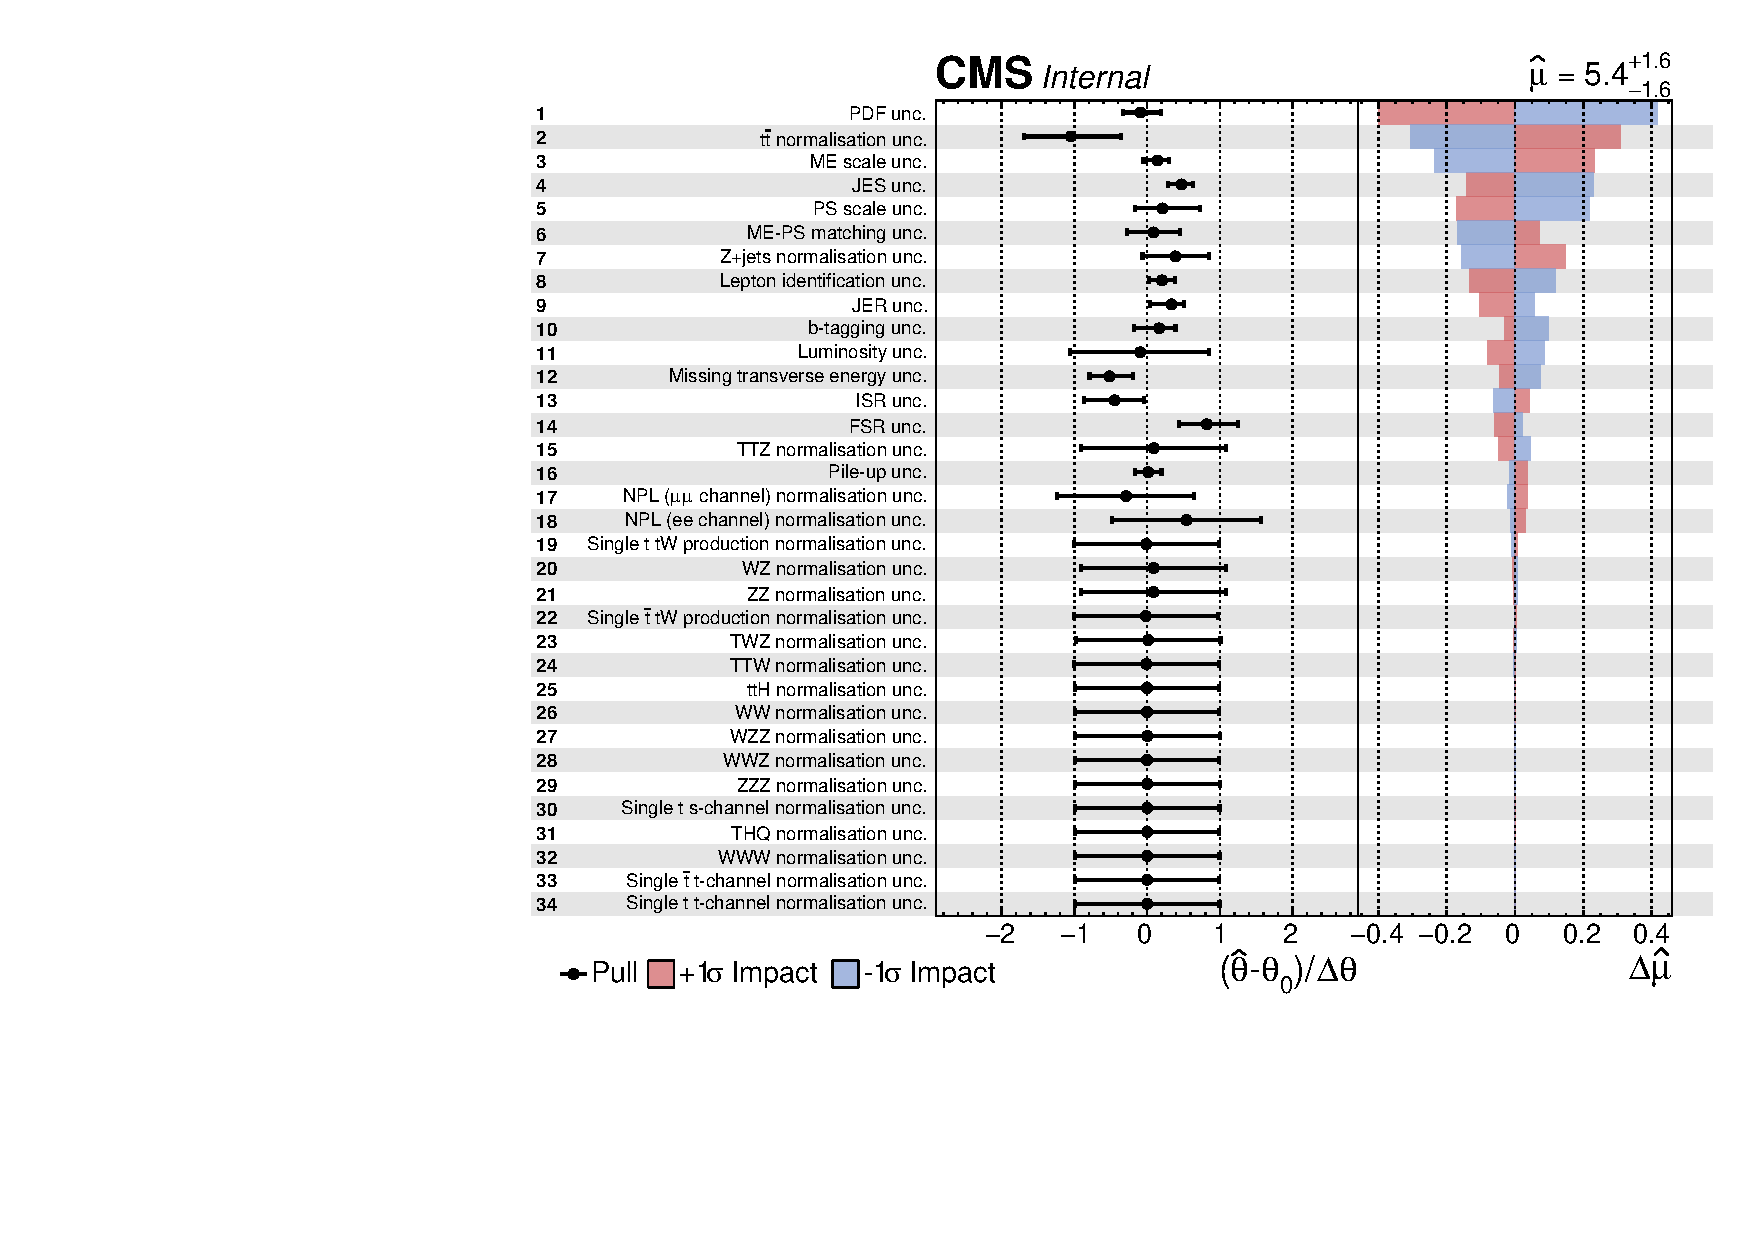
\includegraphics[width=0.97\textwidth]{figs/results/systematicsImpact.pdf}
\caption{The impact of each of the systematic uncertainties considered for the measurement made. The left hand side of the plot shows the residuals of the nuisance parameters, where $\theta$ and $\theta_{0}$ are the post-fit and pre-fit values of the nuisance parameter and $\Delta_{\theta}$ is the pre-fit uncertainty. The right hand side of the plot illustrates the shift in the signal strength parameter induced as a nuisance parameter is fixed and brought to its $\pm \sigma$ post-fit values (with the other parameters profiled as normal).}
\label{fig:systematicsPull}
\end{center}
\end{figure}


\section{Discussion of other searches for tZq at the Large Hadron Collider}
The search for the dilepton final state of a singly produced top in association with a Z boson presented in this thesis is the first one that has been undertaken at the LHC.
As such while these results cannot be directly compared against any previous or competing results, it can be compared against the tZq searches performed for the fully leptonic	final state at $\sqrt{s} = 8 \TeV and 13 \Tev$.

While the first search made for the tZq trilepton final state at $\sqrt{s} = 8 \TeV$ by the CMS collaboration was unable to observe this process, reporting a significance of 2.9 standard deviations~\cite{Sirunyan:2017kkr}, both the ATLAS and CMS collaborations have subsequently performed searches at $\sqrt{s} = 13 \TeV$.
Both the ATLAS and CMS searches have been able to observe the process with reported signifiances of 4.2 and 3.7 standard deviations respectively~\cite{Aaboud:2017ylb,Sirunyan:2017nbr}.

While the $\sqrt{s} = 13 \TeV$ trilepton final state analyses and the dilepton final state analysis presented all use a binned maximum likelihood fit of a multivariate discriminant, the analysis strategies they all employ differ.
Both the trilepton searches use control regions for the backgrounds involving the production of dibosons and top anti-top  quark pairs~\footnote{The ATLAS search used CRs to constrain all diboson processes and \ttbar while the CMS search used CRs to constrain WZ (the dominant diboson background) and \ttbarZ.}, with the reconstructed transverse mass of the W boson used to constrain these processes.
While the lack of a third lepton in the dilepton final state restricts contributions from non-prompt leptons, it also results in the presence of a greater number of significantly larger background processes.
Therefore, despite of 

%%% Discuss details further

Therefore, despite the dilepton final state having a larger production cross section than the fully leptonic final state, the background dominated nature of the final state's topology significantly limits the ability to observe the process.
Even if the inclusion of additional data is insufficient for an observation to be made for the dilepton final state, it should be possible to measure the process with a 5.0 standard deviations significance through combining this measurement with the one made for trilepton final state.


\chapter{Conclusion}\label{chapter:conclusion}
\section{Summary of the tZq analysis}
Following the restart of the LHC in 2015, the LHC's increased centre-of-mass collision energies and instantaneous luminosities have made it possible to undertake measurements of rare processes involving top quark and electroweak interactions.
In this thesis a search was presented for the production of a top quark in association with a Z boson using the dilepton final state using a shape based analysis.
This analysis focussed on understanding and constraining processes that involve the production of two promptly produced leptons that are consistent with a Z boson decay and those that involve at least one non-promptly produced lepton.
A Boosted Decision Tree was used to further enhance the separation between the signal from tZq production and background, using a set of variables that were identified as having the greatest discriminating power.
Using a Maximum Likelihood Fit, signal strengths of $6.213_{-2.695}^{+2.339}$ and $4.725_{-2.015}^{+1.916}$ were measured for the signal process in the $ee$ and $\mu\mu$ channels, respectively.
These measurements correspond to an observed excess over the background-only hypothesis of $2.72\sigma$ and $2.50\sigma$ for the $ee$ and $\mu\mu$ channels, respectively.
Using simulation, the expected significances for the $ee$ and $\mu\mu$ channels and their combination were determined to be $0.46\sigma$, $0.54\sigma$ and $0.70\sigma$, respectively.

These results constitute the first measurement of tZq that has been made using the dilepton final state and are consistent within two standard deviations of the SM prediction and measurements made using the trilepton final state.
Given that these results have not been fully reviewed by the CMS collaboration, further work is required in order to interpret this measurement and to achieve the standard required for journal publication on behalf of the CMS collaboration.

\section{Future measurements}
As the observation of tZq is primarily limited by statistics of the dataset used, the single greatest improvement to the sensitivity of this analysis would be the incorporation of additional data collected by the CMS experiment.
It is anticipated that including the 41.5\fbinv of proton-proton collision data at $\sqrt{s} = 13\TeV$ collected by the CMS experiment during 2017 will improve the expected significance of the result to approximately $1.1\sigma$.
%It is anticipated that an additional X\fbinv of proton-proton collision data at $\sqrt{s} = 13\TeV$ would be required to  improve the expected significance of the result to $3\sigma$.

In addition to including addition data for future measurements, it will be imperative to understand why the observed significance of the measurement presented is considerably larger than the expected significance.
Part of this work will involve ensuring that the Z+jets and \ttbar processes are accurately modelled, including investigating the use of data-driven estimates for these processes and why the Z+jets sample simulated at NLO does not describe data well.
Understanding the largest backgrounds for the analysis is especially pertinent given that it is not currently understood why the nuisance parameters associated with the uncertainty of their cross sections are offset from their pre-fit values to varying degrees in both channels.

The result presented was based on the February 2017 reprocessing of the 2016 data and September 2016 reprocessing of the corresponding simulation samples.
These datasets have subsequently been reprocessed to incorporate updated jet energy corrections and improved alignments and calibrations of the CMS detector.
As such, future measurements will benefit from the improved accuracy of the jet energy scale and resolution corrections of these reprocessed datasets.

Future measurements may potentially benefit from using alternative physics object selection algorithms that have been shown to improve the performance of other CMS analyses.
b-tagging algorithms that use deep neural networks to produce a discriminator have been demonstrated to have higher b-tagging efficiencies, lower misidentification rates and smaller uncertainties than the CSVv2 algorithm used in the analysis presented.
Other analyses have found that MVA-based lepton identification algorithms have lower NPL misidentification rates than the cut-based identification algorithm used in the analysis presented.
While the modelling of the NPL background is not a major limiting factor of the analysis presented, it is not currently known if a MVA-based lepton identification algorithm would be significantly more efficient than the current lepton identification algorithms.

The robustness of the blinding methodology would be improved by parametrising the $\chi^{2}$-like variable so that it better describes the structure present in the $\sigma_{\mathrm{t}}$ and $\sigma_{\mathrm{W}}$ distributions observed in the signal sample and by optimising the values of $\chi^{2}$ used to define the signal and side band regions on the basis of the expected significance of the result in each.

Once an accurate measurement of the tZq cross section can be made, it should be possible to probe the strength of the tZ and WWZ couplings.
Given that tZq production is expected to be as sensitive to the strength of the WWZ coupling as WZ production, this process will provide valuable complimentary measurements of this coupling~\cite{Campbell:2013yla}.

\section{Summary of the TMTT track finding processor system studies}
The \emph{TMTT} collaboration has proposed a track finder system for the CMS tracker at the HL-LHC that is capable of contributing information to the CMS Level-1 trigger.
The \emph{TMTT} track finding system identifies track candidates using time-multiplexed Hough Transforms in the \rphi plane, a Kalman Filter to filter these candidates and precisely fit track parameters to them and a duplicate removal process.
In this thesis a number of studies were presented that were undertaken as part of the development of the this track finding system.

Prior to the hardware demonstrator review in 2016 of the three proposed track finding systems, a linearised $\chi^{2}$ track fitting algorithm was explored as an alternative to the \KF.
The linearised $\chi^{2}$ track fitting algorithm was shown to be capable of both fitting precise helix parameters to the tracks found by the \HT and filtering out hits incorrectly assigned to tracks and incorrectly reconstructed tracks.
Following the evaluation and comparison of both the $\chi^{2}$ track fit algorithm and the \KF, it was decided not to continue development of the former algorithm.
This decision was made as it was determined that the \KF filtering and fitting performance was superior than that of the $\chi^{2}$ track fit, particularly in the forward regions.

The flexibility for the upgraded tracker to be able to reconstruct tracks down to a lower \pT threshold of 2\GeV is potentially desirable and was initially studied as part of the 2016 demonstrator review.
The ability of the proposed track finding system to reconstruct such low transverse momenta tracks ($2\GeV < \pT < 3\GeV$) was shown to be considerably improved by accounting for the effects of \MS. 
For the \HT, this involved using decreased precision \HT cells to mitigate against scattering causing stubs to be found in adjacent cells.
The \KF's covariance matrix was modified to incorporate the uncertainty in the hit position caused by the effects of \MS by including a term that described the average scattering angle as a function of \pT.

\section{Future track finding processor system development}
If the the linearised $\chi^{2}$ track fitting algorithm is to be considered a viable alternative to the other track fitters developed for the \emph{TMTT} project.
While only a small number of track derivatives are required for the calculations in the barrel region, it is uncertain whether there are sufficient resources to tabulate the endcap derivatives required on current hardware.
If it can be demonstrated that current FPGAs can implement this algorithm, it will need to be demonstrated that the $\chi^{2}$ track fitter's performance is competitive with the \KF and \LR.
While it may not be possible to make the $\chi^{2}$ track fitter filter tracks as effectively as the \KF or \LR , other improvements, such including the fitting of the transverse impact parameter, may improve its competitiveness.

Despite the improving the proposed system's ability to reconstruct tracks with low \pT, there are still a number of key areas that require investigating in order to understand the current limitations of the work done so far and how it may be improved upon.
Currently it is not understood why the duplicate rate increases near the boundary between normal and reduced precision \HT cells.
This effect needs to be understood before an optimal value for the cell merging threshold can be determined.
The \KF's performance is likely to be further improved by using a scattering constant term that accurately takes the volume of material a track has passed through into account.
Implementing separate \KF $\chi^{2}$ cuts for the \rphi and \rz planes is another potential improvement given that the dominant uncertainty contribution for the former varies depending on $\pT$.


The \emph{TMTT} collaboration demonstrated in the 2016 review that a complete track finding system for the upgraded CMS tracker that met the baseline system requirements could be built using currently available technology.
Since 2016 the development and optimisation of \emph{TMTT} track finding system has continued using the so-called tilted barrel geometry for anticipated hardware for the final track finding system.
By the end of 2018 it is anticipated that the proposed systems of the \emph{TMTT} and \emph{tracklet} projects will begin to converge to produce an all-FPGA hybrid track finding system.
The final prototype for this all-FPGA track finding system system is anticipated to tested and validated by 2022 in order to ensure a successful installation, integration and commissioning of the upgraded tracker in 2025 prior to the start of HL-LHC operations.

%Given the limited experimental evidence of BSM physics, a large number of BSM physics models, driven by theoretical and ascetic arguments, have been proposed to account for the shortcomings of the SM.
%While the analysis presented in this thesis concerns the search for a SM process, the tZq cross section is sensitive to modifications of the tZ coupling posited by a number of BSM theories.
%
%As eluded to in Section~\ref{subsec:weakForce}, any flavour changing process involving a neutral weak current in the SM cannot occur at the tree level and requires a loop processes involving a virtual W exchange.
%A number of BSM theories however, introduce top quark FCNC decay contributions at the tree level, such as Supersymmetry (SUSY) models and those proposing additional Higgs doublets and/or quark singlets~\cite{AguilarSaavedra:2004wm}.
%The presence of such new tZ couplings would enhance the production rate of both \ttZ and tZq by several orders of magnitude and should be observable at the LHC. 
%As of to date however, no evidence for BSM FCNCs have been observed for the tZ coupling for both single top and \ttbar processes~\cite{Sirunyan:2017kkr}.


\begin{appendices}
\chapter{Maths Notations}\label{app:maths}
This appendix gives the definitions of the Pauli matrices and Dirac matrics~\cite{Cheng:1985bj} used in Chapter~\ref{chapter:theory}.

\section*{Pauli Matrices}

\begin{equation}
\mathbf{\sigma} = ( \sigma_{1}, \sigma_{2}, \sigma_{3} ) \;
\end{equation}

\begin{equation}
\sigma_{1} = \begin{matrix}
0 & 1 \\
1 & 0
\end{matrix} ,
\sigma_{2} = \begin{matrix}
0 & -i \\
i & 0
\end{matrix} ,
\sigma_{3} = \begin{matrix}
1 & 0 \\
0 & -1
\end{matrix}
\end{equation}


\section*{Dirac Matrices}

\begin{equation}
{ {\gamma}^{\mu} , {\gamma}^{\nu} } = 2g^{\mu \nu} \;
\label{eq:gamma}
\end{equation}

where $g^{\mu \nu}$ is the Minkowski metric:

\begin{equation}
g^{\mu \nu} = \pm \begin{matrix}
-1 & 0 & 0 & 0 \\
0 & 1 & 0 & 0 \\
0 & 0 & 1 & 0 \\
0 & 0 & 0 & 1
\end{matrix}
\label{eq:minkowiski}
\end{equation}

\chapter{Data and Simulation Comparison Plots}\label{app:plots}
This appendix contains a selection of comparison plots between data and simulation for the signal region and the \ttbar and Z+jets 0-bjet control regions.
For the signal region and Z+jets control region sections, the left-hand side plots correspond to the $ee$ channel and the right-hand side plots to the $\mu\mu$ channel.

\section{Signal Region}\label{appSec:signalRegionPlots}

\begin{figure}[h]
\centering
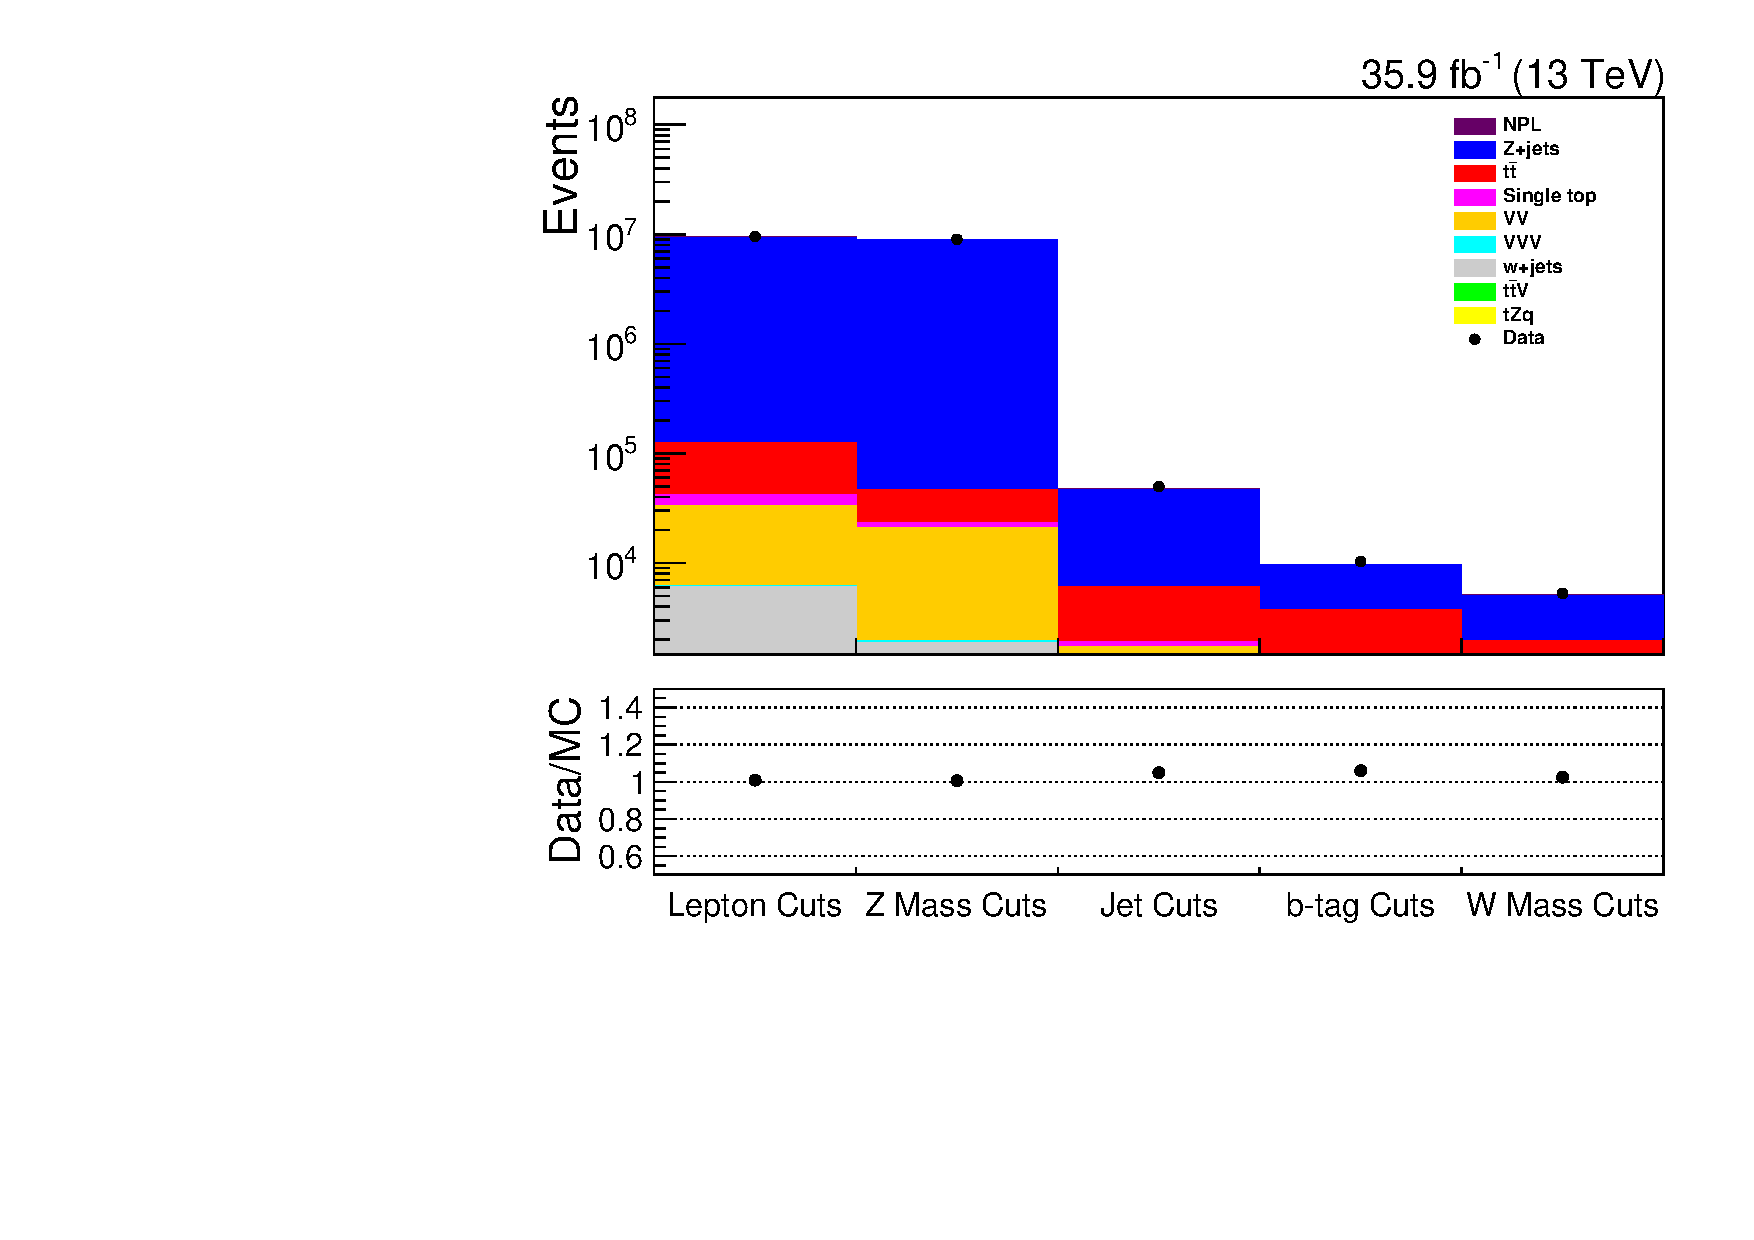
\includegraphics[width=0.97\textwidth]{figs/background-estimation/plots/unblinded/prompt_ee_ttbarInc/cutFlow_log.pdf}
\\
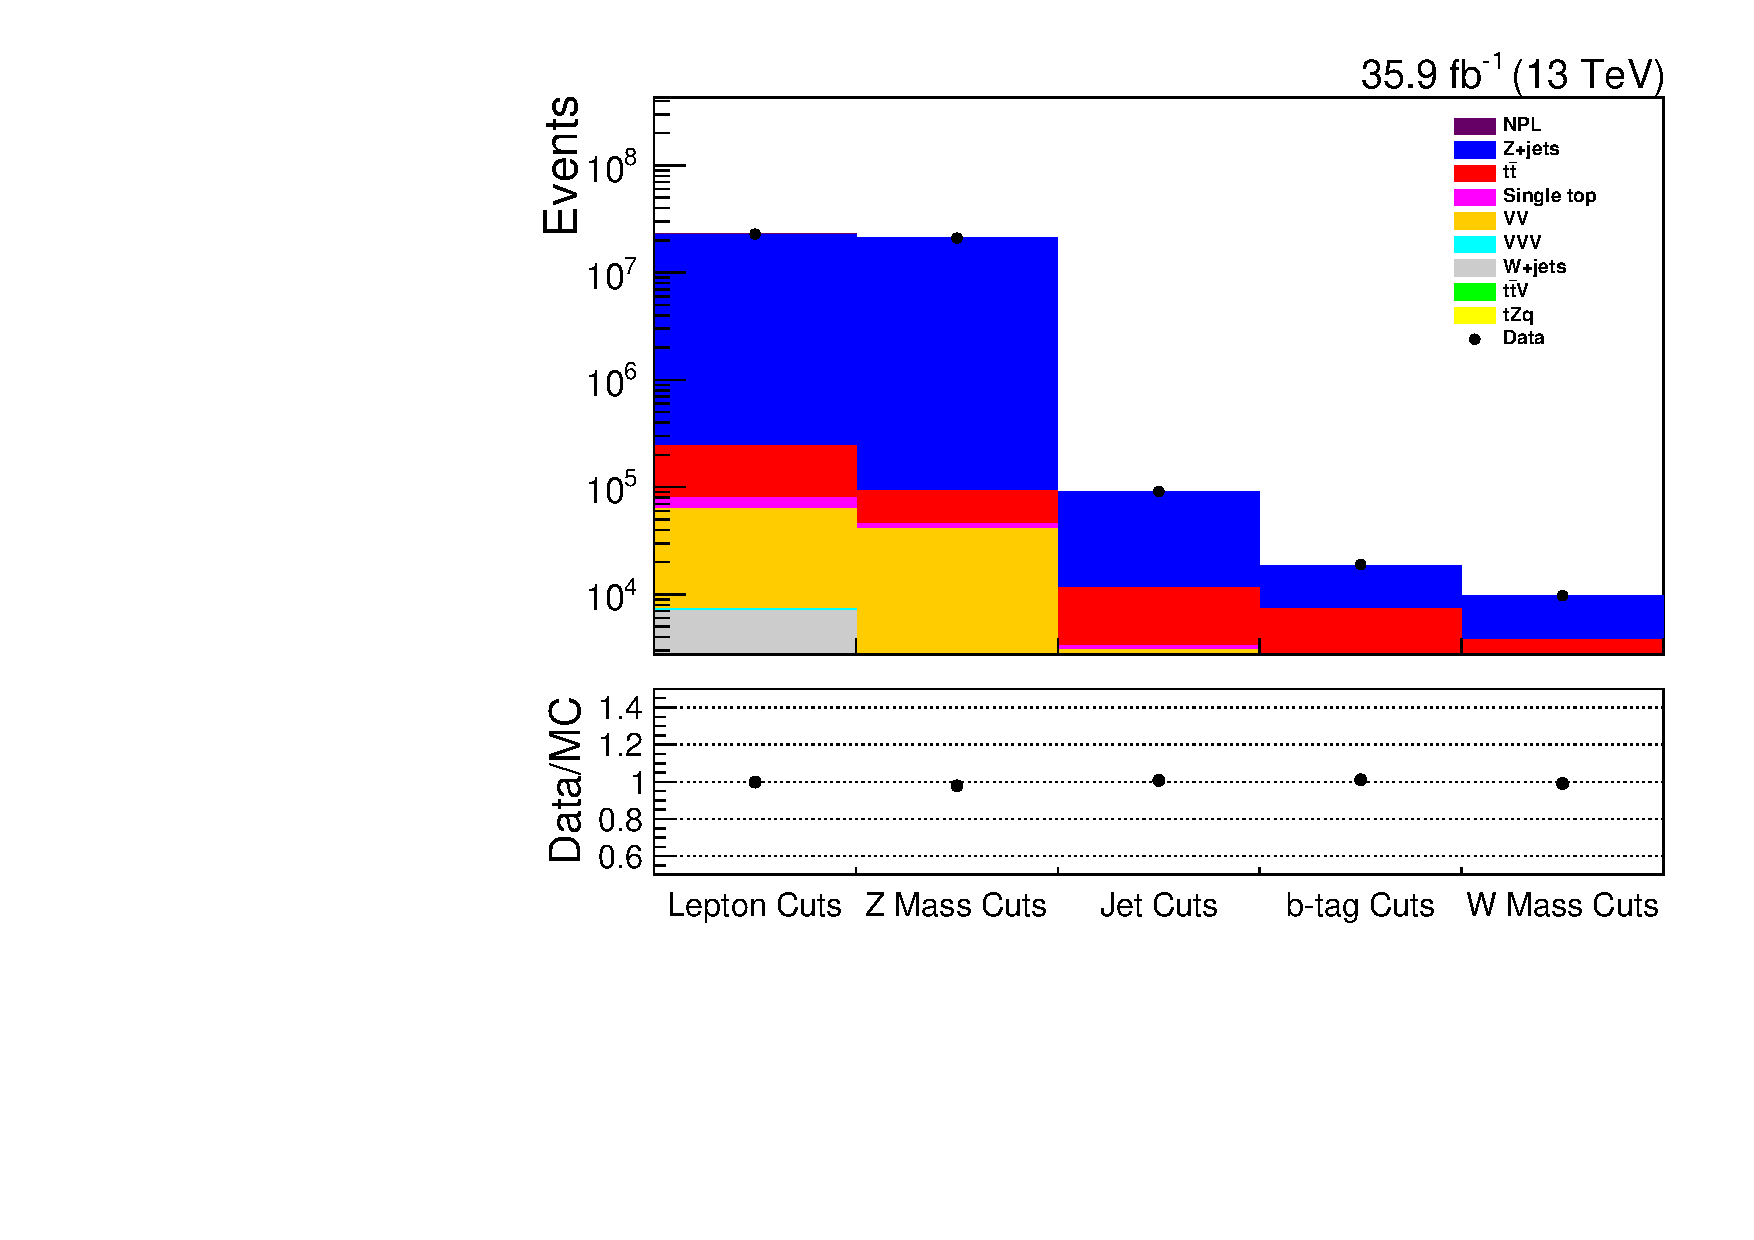
\includegraphics[width=0.97\textwidth]{figs/background-estimation/plots/unblinded/prompt_mumu_ttbarInc/cutFlow_log.pdf}
\caption{
The overall event yield for data and simulation at each stage of applying the signal region selection criteria and simulation corrections.
}
\label{fig:SR_cutFlow}
\end{figure}

\begin{figure}[h]
\centering
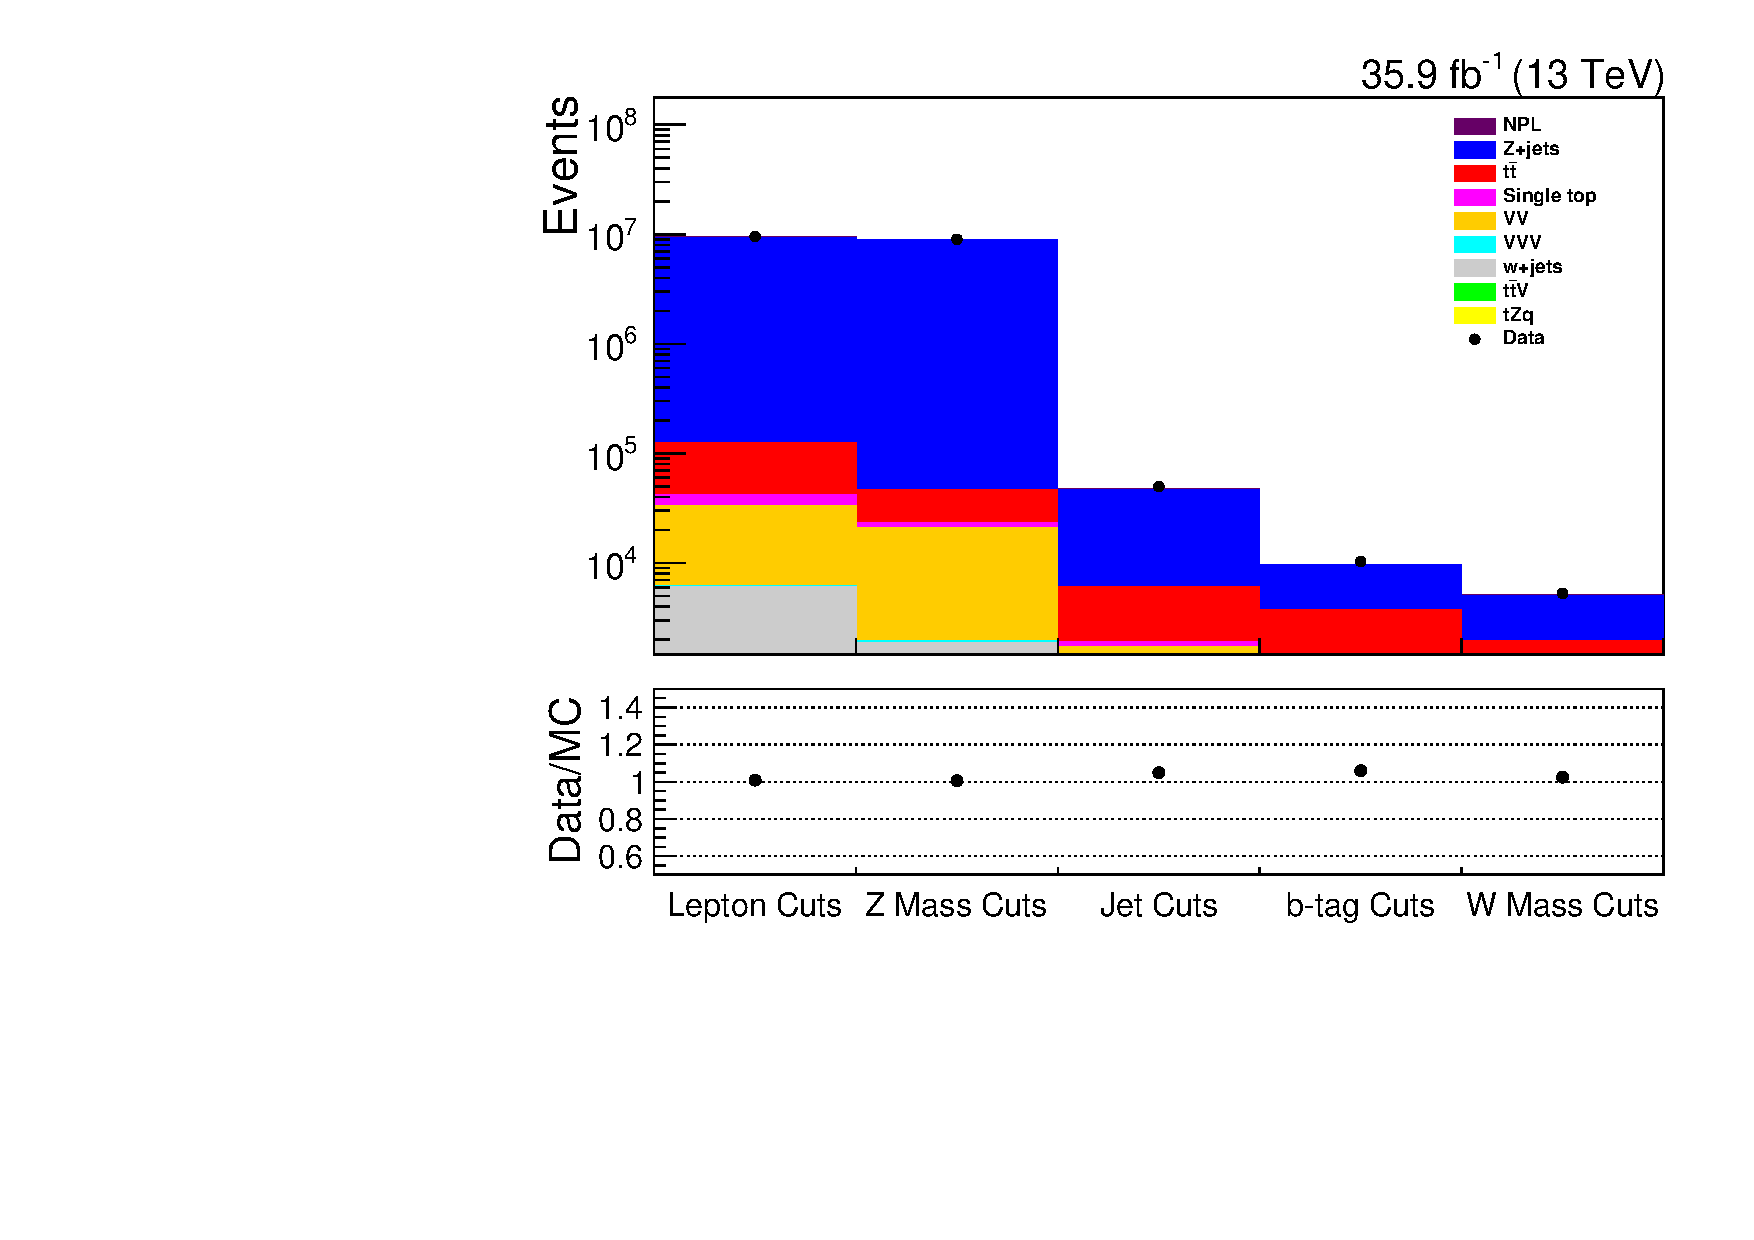
\includegraphics[width=0.47\textwidth]{figs/background-estimation/plots/unblinded/prompt_ee_ttbarInc/cutFlow_log.pdf}
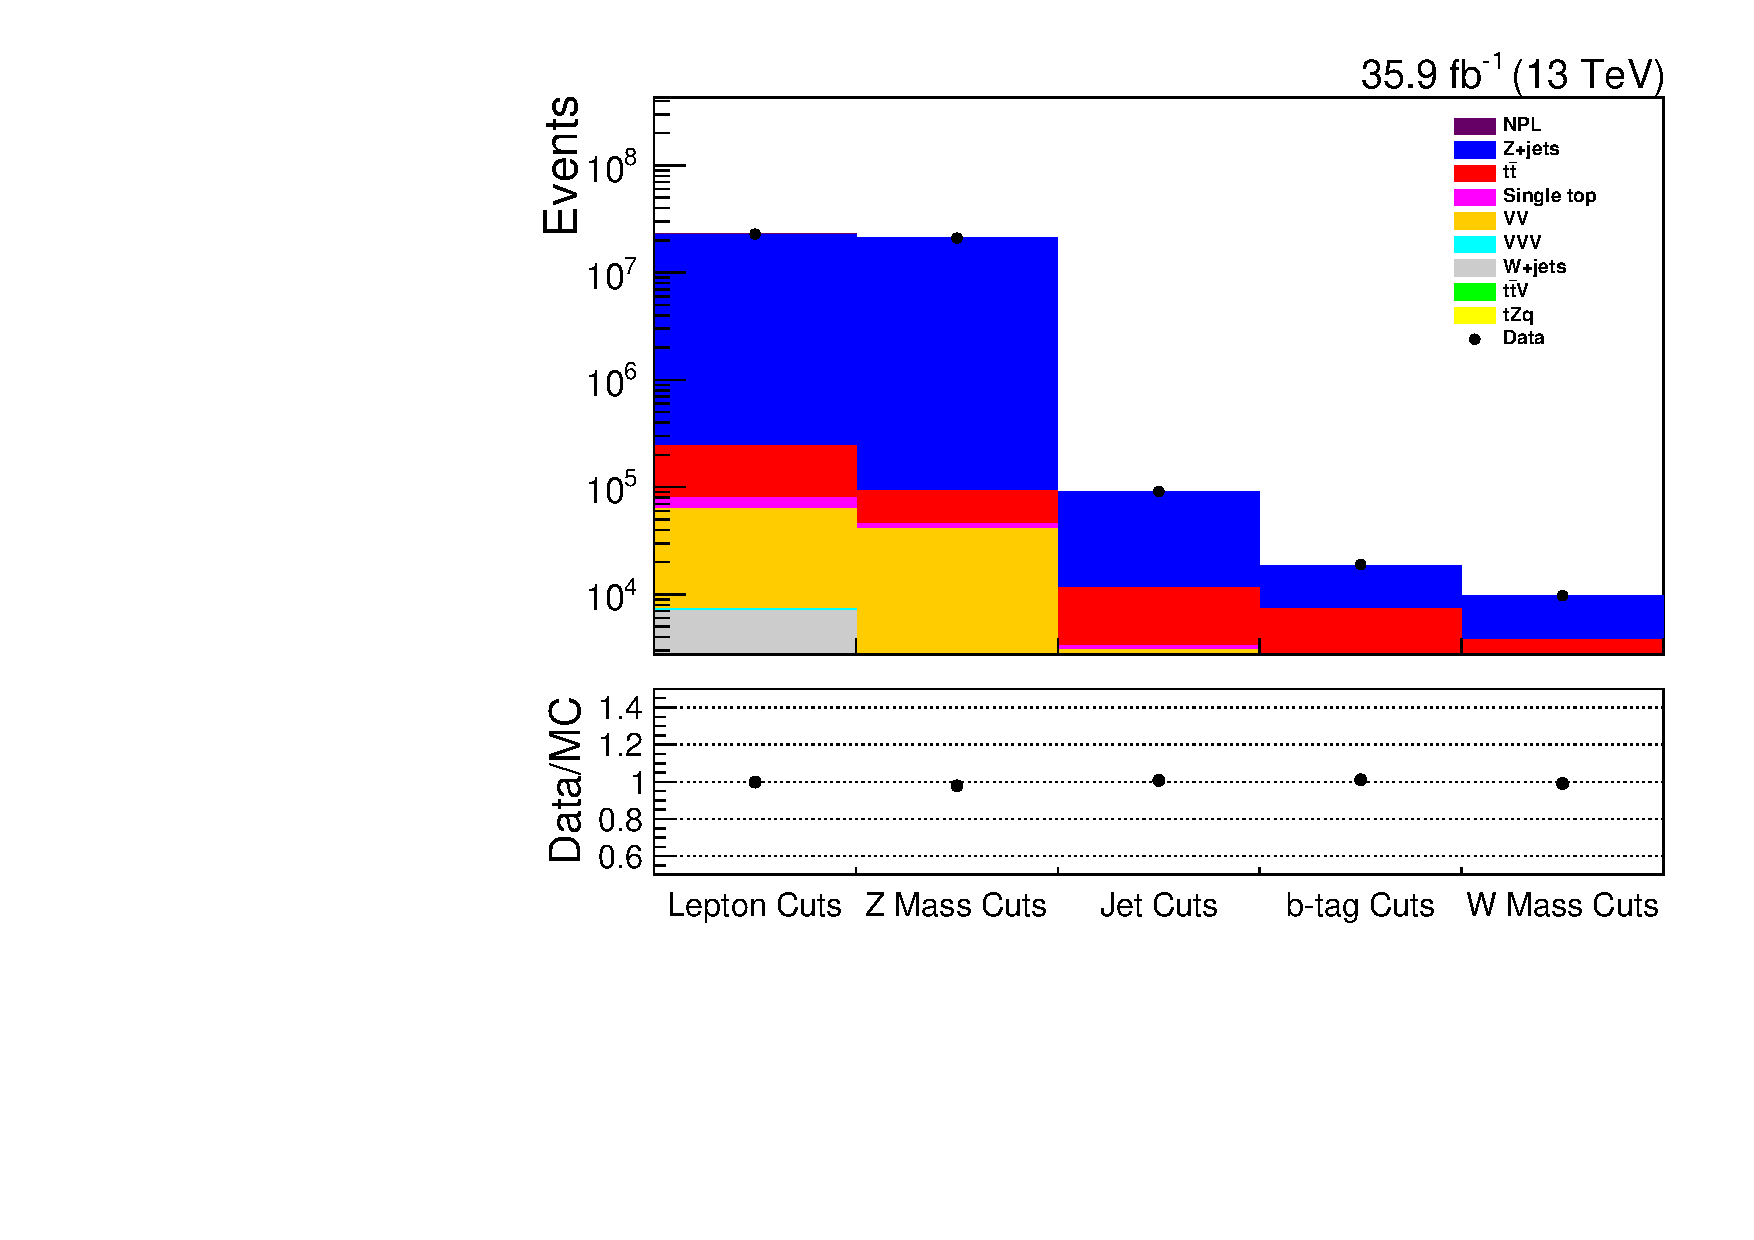
\includegraphics[width=0.47\textwidth]{figs/background-estimation/plots/unblinded/prompt_mumu_ttbarInc/cutFlow_log.pdf}
\\
\caption{
The overall event yield for data and simulation at each stage of applying the signal region selection criteria and simulation corrections for the $ee$ channel (left) and the $\mu\mu$ channel (right).
}
\label{fig:SR_lep1Pt}
\end{figure}

\begin{figure}[h]
\centering
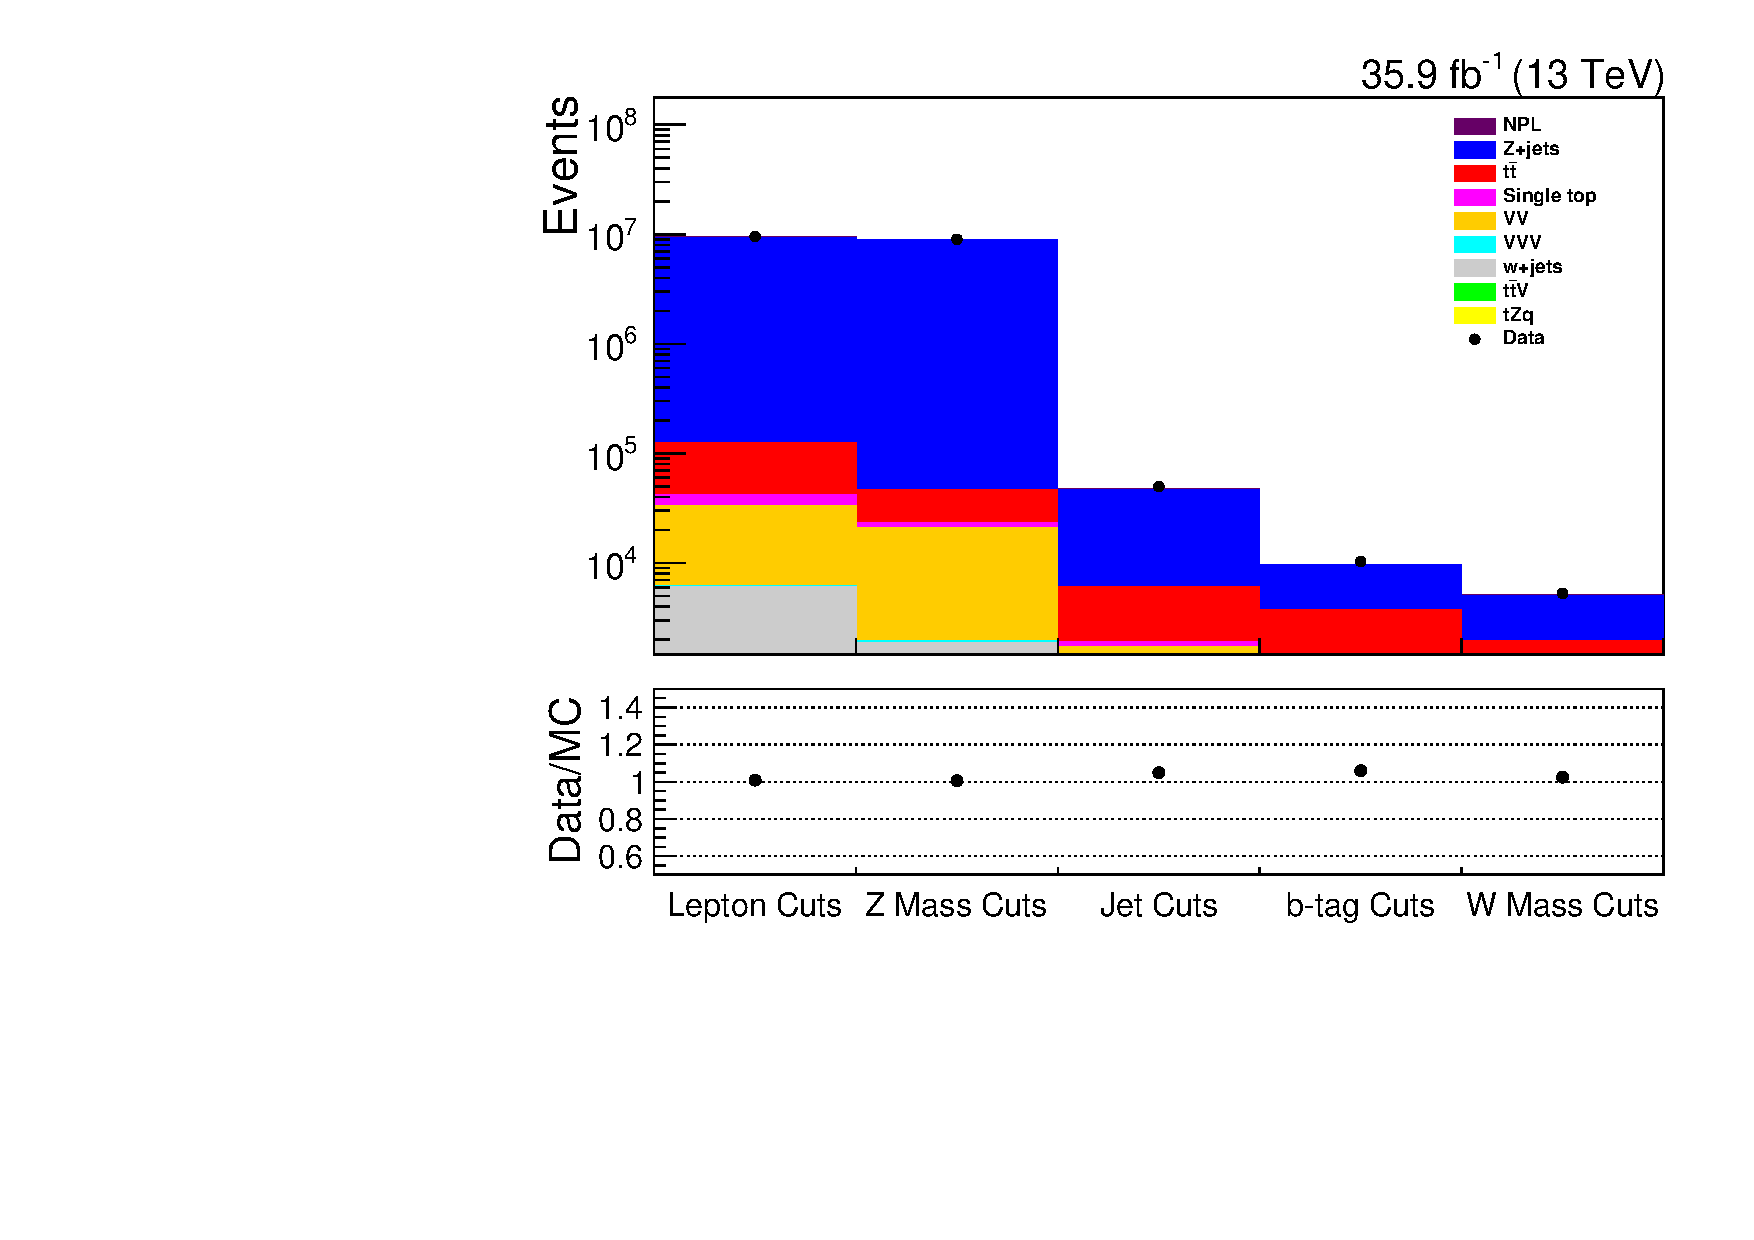
\includegraphics[width=0.47\textwidth]{figs/background-estimation/plots/unblinded/prompt_ee_ttbarInc/cutFlow_log.pdf}
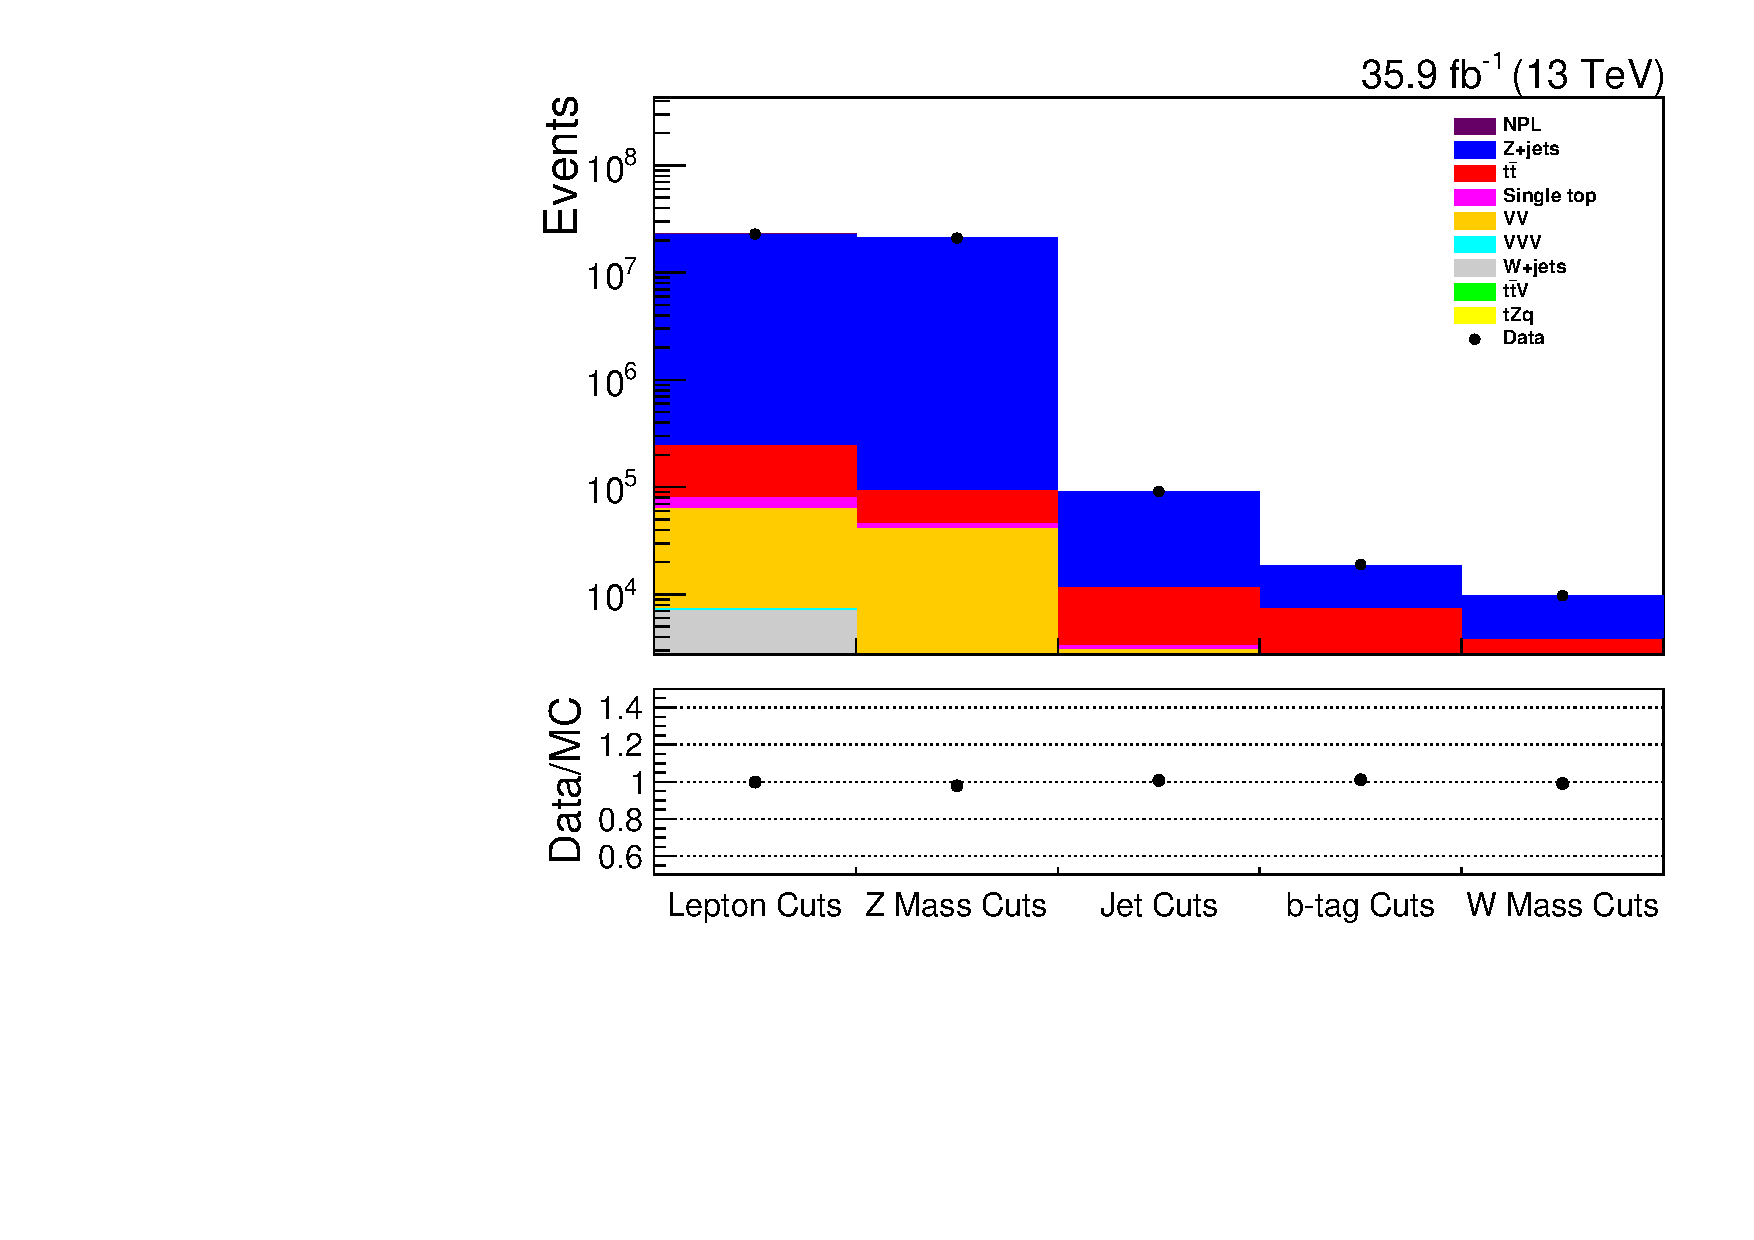
\includegraphics[width=0.47\textwidth]{figs/background-estimation/plots/unblinded/prompt_mumu_ttbarInc/cutFlow_log.pdf}
\caption{
The overall event yield for data and simulation at each stage of applying the signal region selection criteria and simulation corrections for the $ee$ channel (left) and the $\mu\mu$ channel (right).
}
\label{fig:SR_lep2Pt}
\end{figure}

\begin{figure}[h]
\centering
\includegraphics[width=0.47\textwidth]{figs/background-estimation/plots/unblinded/prompt_ee_ttbarInc/cutFlow_log.pdf}
\includegraphics[width=0.47\textwidth]{figs/background-estimation/plots/unblinded/prompt_mumu_ttbarInc/cutFlow_log.pdf}
\caption{
The overall event yield for data and simulation at each stage of applying the signal region selection criteria and simulation corrections for the $ee$ channel (left) and the $\mu\mu$ channel (right).
}
\label{fig:SR_lep1Eta}
\end{figure}

\begin{figure}[h]
\centering
\includegraphics[width=0.47\textwidth]{figs/background-estimation/plots/unblinded/prompt_ee_ttbarInc/cutFlow_log.pdf}
\includegraphics[width=0.47\textwidth]{figs/background-estimation/plots/unblinded/prompt_mumu_ttbarInc/cutFlow_log.pdf}
\caption{
The overall event yield for data and simulation at each stage of applying the signal region selection criteria and simulation corrections for the $ee$ channel (left) and the $\mu\mu$ channel (right).
}
\label{fig:SR_lep2Eta}
\end{figure}

\section{Z+jets Control Region}\label{appSec:signalRegionPlots}

\section{\ttbar Control Region}\label{appSec:signalRegionPlots}

\begin{figure}[h]
\centering
\includegraphics[width=0.97\textwidth]{figs/background-estimation/plots/unblinded/ttbar_control/cutFlow_log.pdf}
\caption{
The overall event yield for data and simulation at each stage of applying the signal region selection criteria and simulation corrections.
}
\label{fig:ttbar_cutFlow}
\end{figure}

\begin{figure}[h]
\centering
\includegraphics[width=0.47\textwidth]{figs/background-estimation/plots/unblinded/prompt_ee_ttbarInc/cutFlow_log.pdf}
\includegraphics[width=0.47\textwidth]{figs/background-estimation/plots/unblinded/prompt_mumu_ttbarInc/cutFlow_log.pdf}
\\
\includegraphics[width=0.47\textwidth]{figs/background-estimation/plots/unblinded/prompt_ee_ttbarInc/cutFlow_log.pdf}
\includegraphics[width=0.47\textwidth]{figs/background-estimation/plots/unblinded/prompt_mumu_ttbarInc/cutFlow_log.pdf}
\caption{
The electron \pT (left) and $\eta$ following applying the lepton selection criteria (top) and the jet selection criteria (bottom).
}
\label{fig:ttbar_electron}
\end{figure}

\begin{figure}[h]
\centering
\includegraphics[width=0.47\textwidth]{figs/background-estimation/plots/unblinded/prompt_ee_ttbarInc/cutFlow_log.pdf}
\includegraphics[width=0.47\textwidth]{figs/background-estimation/plots/unblinded/prompt_mumu_ttbarInc/cutFlow_log.pdf}
\\
\includegraphics[width=0.47\textwidth]{figs/background-estimation/plots/unblinded/prompt_ee_ttbarInc/cutFlow_log.pdf}
\includegraphics[width=0.47\textwidth]{figs/background-estimation/plots/unblinded/prompt_mumu_ttbarInc/cutFlow_log.pdf}
\caption{
The muon \pT (left) and $\eta$ following applying the lepton selection criteria (top) and the jet selection criteria (bottom).
}
\label{fig:ttbar_muon}
\end{figure}
\chapter{Further information regarding Boosted Decision Trees}\label{app:bdt}

\section{BDT Input Features}\label{appsec:bdtFeatures}
The variables listed in table~\ref{allBdtVariables}

\begin{table}[htbp]
\topcaption {The name and descriptions of the variables chosen by recursive feature elimination to be used as input to the BDT to discriminate between potential tZq signal events and the dominant backgrounds.
}
\label{tab:allBdtVariables}
  \centering
% This increases column spacing.
\resizebox{\textwidth}{!}{
% This right-aligns numbers in column, but centers them under column title.
\begin{tabular}{cccc}
   \hline
   \textbf{Variable} & \textbf{Description} \\
   \hline
    wQuark1Pt & Leading W boson candidate jet \pt \\
    wQuark1Eta & Leading W boson candidate jet $\eta$ \\
    wQuark1Phi &  Leading W boson candidate jet $\phi$ \\
    wQuark2Pt & Subleading W boson candidate jet \pt \\
    wQuark2Eta & Subleading W boson candidate jet $\eta$ \\
    wQuark2Phi & Subleading W boson candidate jet $\phi$  \\
    wPairMass & W boson mass  \\
    wPairPt & W boson \pt  \\
    wPairEta & W boson $\eta$  \\
    wPairPhi & W boson $\phi$  \\
    mTW & W boson $m_{T}$  \\
    met & \met  \\
    nJets & Number of jets  \\
    leadJetPt & Leading jet \pt $\checkmark$ \\
    leadJetPhi & Leading jet $\phi$  \\
    leadJetEta & Leading jet $\eta$  \\
    leadJetbTag & Leading jet b-tag discriminator  \\
    secJetPt & Subleading jet \pt \\
    secJetPhi & Subleading jet $\phi$  \\
    secJetEta & Subleading jet $\eta$ \\
    secJetbTag & Subleading jet b-tag discriminator  \\
    thirdJetPt & Third jet \pt \\
    thirdJetPhi & Third jet $\phi$  \\
    thirdJetEta & Third jet $\eta$ \\
    thirdJetbTag & Third jet b-tag discriminator  \\
    fourthJetPt & Fourth jet \pt \\
    fourthJetPhi & Fourth jet $\phi$  \\
    fourthJetEta & Fourth jet $\eta$ \\
    fourthJetbTag & Fourth jet b-tag discriminator  \\
    nBjets & Number of b-tagged jets \\
    bTagDisc & Leading b-tagged jet b-tag discriminator \\
    lep1Pt & Leading lepton \pt \\
    lep1Eta & Leading lepton $\eta$ \\
    lep1Phi & Leading lepton $\phi$ \\
    lep1RelIso & Leading lepton $I^{rel}$ \\
    lep1D0 & Leading lepton $d_{0}$ \\
    lep2Pt & Subleading lepton \pt \\
    lep2Eta & Subleading lepton $\eta$ \\
    lep2Phi & Subleading lepton $\phi$ \\
    lep2RelIso & Subleading lepton $I^{rel}$ \\
    lep2D0 & Subleading lepton $d_{0}$ \\
    zMass & Z boson mass  \\
    zPt & Z boson \pt \\
    zEta & Z boson $\eta$ \\
    zPhi & Z boson $\phi$ \\
    topMass & Top quark mass \\
    topPt & Top quark \pt \\
    topEta & Top quark $\eta$ \\
    topPhi & Top quark $\phi$ \\
    j1j2delR & $\Delta R$ between the leading and subleading jets \\
    j1j2delPhi & $\Delta \phi$ between the leading and subleading jets \\
    w1w2delR & $\Delta R$ between the W boson jets \\
    w1w2delPhi & $\Delta \phi$ between the W boson jets \\
    zLepdelR & $\Delta R$ between the Z boson leptons \\
    zLepdelPhi & $\Delta \phi$ between the Z boson leptons \\
    zl1Quark1DelR & $\Delta R$ between the leading lepton and leading W boson jet \\
    zl1Quark1DelPhi & $\Delta \phi$ between the leading lepton and leading W boson jet \\
    zl1Quark2DelR & $\Delta R$ between the leading lepton and subleading W boson jet \\
    zl1Quark2DelPhi & $\Delta \phi$ between the leading lepton and subleading W boson jet \\
    zl2Quark1DelR & $\Delta R$ between the subleading lepton and leading W boson jet \\
    zl2Quark1DelPhi & $\Delta \phi$ between the subleading lepton and leading W boson jet \\
    zl2Quark2DelR & $\Delta R$ between the subleading lepton and subleading W boson jet \\
    zl2Quark2DelPhi & $\Delta \phi$ between the subleading lepton and leading W boson jet \\
    zlb1DelR & $\Delta R$ between the Z boson and leading b-tagged jet \\
    zlb1DelPhi & $\Delta \phi$ between the Z boson and leading b-tagged jet \\
    zlb2DelR & $\Delta R$ between the Z boson and subleading b-tagged jet\\
    zlb2DelPhi & $\Delta \phi$ between the Z boson and subleading b-tagged jet \\
    lepHt & ${\ensuremath{H_{\mathrm{T}}}$ of the Z boson leptons \\
    wQuarkHt & ${\ensuremath{H_{\mathrm{T}}}$ of the W boson quarks \\
    totPtVec & \pt of the system \\
    totEta & $\eta$ of the system \\
    totPhi & $\phi$ of the system \\
    totVecM & Invariant mass of the system \\
    totPt2Jet & Square of the sum of the two leading jets' \pT \\
    totJetPt & Sum of all the jets' \pT  \\
    wZdelR & $\Delta R$ between the W and Z bosons \\
    wZdelPhi & $\Delta \phi$ between the W and Z bosons \\
    zQuark1DelR & $\Delta R$ between the Z boson and leading W boson jet \\
    zQuark1DelPhi & $\Delta \phi$ between the Z boson and leading W boson jet \\
    zQuark2DelR & $\Delta R$ between the Z boson and subleading W boson jet \\
    zQuark2DelPhi & $\Delta \phi$ between the Z boson and subleading W boson jet \\
    zTopDelR & $\Delta R$ between the Z boson and top quark \\
    zTopDelPhi & $\Delta \phi$ between the Z boson and top quark\\
    zl1TopDelR & $\Delta R$ between the leading lepton and top quark \\
    zl1TopDelPhi & $\Delta \phi$ between the leading lepton and top quark \\
    zl2TopDelR & $\Delta R$ between the subleading lepton and top quark \\
    zl2TopDelPhi & $\Delta \phi$ between the subleading lepton and top quark \\
    wTopDelR & $\Delta R$ between the W boson and top quark \\
    wTopDelPhi & $\Delta \phi$ between the W boson and top quark \\
    w1TopDelR & $\Delta R$ between the leading W boson jet and top quark \\
    w1TopDelPhi & $\Delta \phi$ between the leading W boson jet and top quark \\
    w2TopDelR & $\Delta R$ between the subleading W boson jet and top quark \\
    w2TopDelPhi & $\Delta \phi$ between the subleading W boson jet and top quark \\
    zjminR & Minimum $\Delta R$ between the Z boson and a jet  \\
    minZJetPhi & Minimum $\phi R$ between the Z boson and a jet \\
    totHt & Total ${\ensuremath{H_{\mathrm{T}}}$ of the system \\
    jetHt & ${\ensuremath{H_{\mathrm{T}}}$ of all the jets present \\
    jetMass & Invariant mass of all the jets present \\
    jetPt & \pT of all the jets present \\
    jetEta & $\eta$ of all the jets present \\
    jetPhi & $\phi$ of all the jets present \\
    jetMass3 & Invariant mass of the leading three jets\\
    totHtOverPt & Total ${\ensuremath{H_{\mathrm{T}}}$ divided by the system's \pT \\
   \hline
 \end{tabular}}
\end{table}

\end{appendices}

\bibliographystyle{JHEP}
\bibliography{admorton_thesis}
 
\end{document}
